\documentclass[a4paper,11pt]{book}

% \newcommand{\Home}{/Users/kannan/FOSS/scilab-arduino/floss-arduino-clone}
% \newcommand{\Origin}{/Users/kannan/FOSS/scilab-arduino/floss-arduino-clone}

\newcommand{\Home}{/home/fossee/Desktop/FLOSS-Arduino-Book}
\newcommand{\Origin}{/home/fossee/Desktop/FLOSS-Arduino-Book}

\newcommand{\bluecolor}[1]{\color{blue}#1\color{black}}
\usepackage{color}
\usepackage{layouts}
%\usepackage{ccicons}
\usepackage{morefloats}
\usepackage{paralist}
\usepackage{chngcntr}
\usepackage{layouts}
\usepackage{fancyhdr}
\pagestyle{headings}
\usepackage{amsmath,graphicx,makeidx}
\usepackage{fancybox}
\usepackage{cite}
\usepackage{hyperref}
%\usepackage{appendix}
\counterwithout{footnote}{chapter}
\usepackage{subfig}
\usepackage{listings}
\usepackage{varioref} % for \vref commands
%\usepackage{hyperref}

%\DeclareFontFamily{OT1}{cmtt}{\hyphenchar \font=-1}
\usepackage[T1]{fontenc}
\usepackage{beramono}
\usepackage{seqsplit}

\newcommand{\portcmd}{\small%
, see \fnrefp{fn:port}}

\newcommand{\redcolor}[1]{\color{red}#1\color{black}}
\newcommand{\codclr}{10pt}
\newcommand{\scilab}{Scilab}
\newcommand{\arduino}{Arduino Uno}
\newcommand{\ie}{\emph{i.e.},}

\newcommand{\ourname}[1]{\\ [1.5mm] \noindent{\bf #1}}
% Shroff book size
%\textheight 7.75in
\textheight 7.5in
\textwidth 5.5in
\evensidemargin 0.625in
\oddsidemargin 0.625in


% code environment
\usepackage{ntheorem}
{\theorembodyfont{\rmfamily} \newtheorem{codemass}{Scilab Code}[chapter]}
\newenvironment{scicode}%
{\begin{codemass}}{\hrule \end{codemass}}

% create listing for code

\newcommand\ccaption[1]
     {\addcontentsline{cod}{section}{\protect\numberline {\thecodemass}#1}}
\makeatletter \newcommand\listofcode
     {\chapter*{List of Scilab, Python, Julia \& OpenModelica Code\markboth%
                        {\bf List of Scilab, Python, Julia \& OpenModelica Code}{}}%
\renewcommand*\l@section{\@dottedtocline{1}{1.5em}{3em}}%
\addcontentsline{toc}{chapter}{\protect\numberline{List of Scilab, Python, Julia \& OpenModelica Code}}
\@starttoc{cod}}
\newcommand\l@scilab[3]
     {#1 \par\noindent#2, #3 \par} 
\renewcommand\@pnumwidth{2.1em}
\makeatother

\usepackage{ntheorem}
{\theorembodyfont{\rmfamily} \newtheorem{ardmass}{Arduino Code}[chapter]}

\newenvironment{ardcode}%
{\begin{ardmass}}{\hrule \end{ardmass}}

\newcommand\acaption[1]
     {\addcontentsline{ard}{section}{\protect\numberline {\theardmass}#1}}

\makeatletter \newcommand\listofard
     {\chapter*{List of Arduino Code\markboth%
                        {\bf List of Arduino Code}{}}%
\renewcommand*\l@section{\@dottedtocline{1}{1.5em}{3em}}%
\addcontentsline{toc}{chapter}{\protect\numberline{List of Arduino \ Code}}
\@starttoc{ard}}
\newcommand\l@arduino[3]
     {#1 \par\noindent#2, #3 \par} 
\renewcommand\@pnumwidth{2.1em}
\makeatother

%%%%%%%%%%python
\usepackage{ntheorem}
{\theorembodyfont{\rmfamily} \newtheorem{pymass}{Python Code}[chapter]}
\newenvironment{pycode}%
{\begin{pymass}}{\hrule \end{pymass}}

% create listing for code

\newcommand\pcaption[1]
     {\addcontentsline{cod}{section}{\protect\numberline {\thepymass}#1}}
\makeatletter \newcommand\listofpyd
     {\chapter*{List of Python Code\markboth%
                        {\bf List of Python Code}{}}%
\renewcommand*\l@section{\@dottedtocline{1}{1.5em}{3em}}%
\addcontentsline{toc}{chapter}{\protect\numberline{List of Python \ Code}}
\@starttoc{pyd}}
\newcommand\l@python[3]
     {#1 \par\noindent#2, #3 \par} 
\renewcommand\@pnumwidth{2.1em}
\makeatother
%%%%%%%%%python

%%%%%%%%%%julia
\usepackage{ntheorem}
{\theorembodyfont{\rmfamily} \newtheorem{juliamass}{Julia Code}[chapter]}
\newenvironment{juliacode}%
{\begin{juliamass}}{\hrule \end{juliamass}}

% create listing for code

\newcommand\jcaption[1]
     {\addcontentsline{cod}{section}{\protect\numberline {\thejuliamass}#1}}
\makeatletter \newcommand\listofjuliad
     {\chapter*{List of Julia Code\markboth%
                        {\bf List of Julia Code}{}}%
                        %{\bf List of Julia Code}{}}%
\renewcommand*\l@section{\@dottedtocline{1}{1.5em}{3em}}%
\addcontentsline{toc}{chapter}{\protect\numberline{List of Julia\ Code}}
\@starttoc{juliad}}
\newcommand\l@julia[3]
     {#1 \par\noindent#2, #3 \par} 
\renewcommand\@pnumwidth{2.1em}
\makeatother
%%%%%%%%%julia

%%%%%%%%%%OpenModelica
\usepackage{ntheorem}
{\theorembodyfont{\rmfamily} \newtheorem{OpenModelicamass}{OpenModelica Code}[chapter]}
\newenvironment{OpenModelicacode}%
{\begin{OpenModelicamass}}{\hrule \end{OpenModelicamass}}

% create listing for code

\newcommand\mcaption[1]
     {\addcontentsline{cod}{section}{\protect\numberline {\theOpenModelicamass}#1}}
\makeatletter \newcommand\listofOpenModelicad
     {\chapter*{List of OpenModelica Code\markboth%
                        {\bf List of OpenModelica Code}{}}%
                        %{\bf List of Julia Code}{}}%
\renewcommand*\l@section{\@dottedtocline{1}{1.5em}{3em}}%
\addcontentsline{toc}{chapter}{\protect\numberline{List of OpenModelica\ Code}}
\@starttoc{OpenMOdelicad}}
\newcommand\l@OpenModelica[3]
     {#1 \par\noindent#2, #3 \par} 
\renewcommand\@pnumwidth{2.1em}
\makeatother
%%%%%%%%%OpenModelica


\makeatletter
\renewcommand\tableofcontents{%
    \if@twocolumn
      \@restonecoltrue\onecolumn
    \else
      \@restonecolfalse
    \fi
    \chapter*{\contentsname
        \@mkboth{%
           \bf \contentsname}{\bf \contentsname}}%
    \@starttoc{toc}%
    \if@restonecol\twocolumn\fi
    }
%
\renewcommand\listoffigures{%
    \if@twocolumn
      \@restonecoltrue\onecolumn
    \else
      \@restonecolfalse
    \fi
    \chapter*{\listfigurename
        \@mkboth{%
           \bf \listfigurename}{\bf \listfigurename}}%
\addcontentsline{toc}{chapter}{\protect\numberline{List of Figures}}
    \@starttoc{lof}%
    \if@restonecol\twocolumn\fi
    }
%
\renewcommand\listoftables{%
    \if@twocolumn
      \@restonecoltrue\onecolumn
    \else
      \@restonecolfalse
    \fi
    \chapter*{\listtablename
        \@mkboth{%
           \bf \listtablename}{\bf \listtablename}}%
\addcontentsline{toc}{chapter}{\protect\numberline{List of Tables}}
    \@starttoc{lot}%
    \if@restonecol\twocolumn\fi
    }
%
\renewenvironment{theindex}
               {\if@twocolumn
                  \@restonecolfalse
                \else
                  \@restonecoltrue
                \fi
                \columnseprule \z@
                \columnsep 35\p@
                \twocolumn[\@makeschapterhead{\indexname}]%
                \@mkboth{\bf \indexname}%
                        {\bf \indexname}%
\addcontentsline{toc}{chapter}{\protect\numberline{\indexname}}%
                \thispagestyle{plain}\parindent\z@
                \parskip\z@ \@plus .3\p@\relax
                \let\item\@idxitem}
               {\if@restonecol\onecolumn\else\clearpage\fi}
\renewenvironment{thebibliography}[1]
     {\chapter*{\bibname}%
      \@mkboth{\bf \bibname}{\bf \bibname}%
\addcontentsline{toc}{chapter}{\protect\numberline{References}}%
      \list{\@biblabel{\@arabic\c@enumiv}}%
           {\settowidth\labelwidth{\@biblabel{#1}}%
            \leftmargin\labelwidth
            \advance\leftmargin\labelsep
            \@openbib@code
            \usecounter{enumiv}%
            \let\p@enumiv\@empty
            \renewcommand\theenumiv{\@arabic\c@enumiv}}%
      \sloppy
      \clubpenalty4000
      \@clubpenalty \clubpenalty
      \widowpenalty4000%
      \sfcode`\.\@m}
     {\def\@noitemerr
       {\@latex@warning{Empty `thebibliography' environment}}%
      \endlist}
\makeatother

%\makeatletter
%\renewcommand{\p@subfigure}{}
%\renewcommand{\@thesubfigure}{\thesubfigure:\hskip\subfiglabelskip}
%\makeatother
%\setcounter{lofdepth}{2}

%\makeatletter\renewcommand{\p@subfigure}{}\renewcommand{\@thesubfigure}{\thesubfigure:\hskip\subfiglabelskip}\makeatother

%\setcounter{lofdepth}{2}

\lstdefinestyle{mystyle}{
    numberstyle=\tiny,
    basicstyle=\footnotesize,
    breakatwhitespace=false,         
    breaklines=true,                 
    captionpos=b,                    
    keepspaces=true,                 
    numbers=left,                    
    numbersep=5pt,                  
    showspaces=false,                
    showstringspaces=false,
    showtabs=false,                  
    tabsize=2
}

\lstset{style=mystyle,language=Scilab,numbers=left,numberstyle=\tiny,
  breaklines,commentstyle=\scriptsize}

\lstdefinestyle{nonumbers}{
    numbers=none,
    basicstyle=\footnotesize,
    breakatwhitespace=false,         
    breaklines=true,                 
    captionpos=b,                    
    keepspaces=true,                 
    showspaces=false,                
    showstringspaces=false,
    showtabs=false,                  
    tabsize=2
}

\lstset{style=mystyle,language=C,numbers=left,numberstyle=\tiny,
  breaklines,commentstyle=\scriptsize}

\newenvironment{indented}[1][]%
               {\list{}%
                {\leftmargin \parindent%
                 \rightmargin \parindent%
                 \labelsep   1em%
                 \itemindent 0in}%
                \item#1\relax}%
               {\endlist\noindent}%
\def\eop{ \hbox{{\vrule height7pt width3pt depth0pt}}}
\def\qed{\hspace*{\fill}\eop}

\newenvironment{thmenumerate}{%
\leavevmode\vspace{-1.4em}
\begin{enumerate}[label=(\arabic*),leftmargin=*,align=left]
}{%
\end{enumerate}
}

\usepackage{theorem}
{\theorembodyfont{\sffamily} \newtheorem{egmass}{Exercise}[chapter]}
\newenvironment{exercise}%
{\begin{indented}\begin{egmass} }{\end{egmass} \vspace{-2ex} \qed%
\end{indented}} 

\renewcommand\chaptermark[1]{\markboth{\bf {\thechapter. #1}}{}}
\renewcommand\sectionmark[1]{\markright{\bf {\thesection. #1}}}
\cfoot{}
\fancyfoot{}

\newcommand{\comment}[1]{\color{red}#1\color{black}}
\newcommand{\eatcomment}[0]{\renewcommand{\reminder}[1]{}}


\newcommand{\tnfig}{0.3\linewidth}
\newcommand{\smfig}{0.45\linewidth}%0.42
\newcommand{\smfigp}{0.49\linewidth}%0.42
\newcommand{\lgfig}{0.65\linewidth}%0.65
\newcommand{\hgfig}{0.9\linewidth}

\renewcommand\bibname{References}

\newcommand{\figref}[1]{Fig.~\ref{#1}}
\newcommand{\figrefp}[1]{Fig.~\vref{#1}}
\newcommand{\tabref}[1]{Table~\ref{#1}}
\newcommand{\tabrefp}[1]{Table~\vref{#1}}
\newcommand{\chapref}[1]{Chapter~\ref{#1}}
\newcommand{\secref}[1]{Sec.~\ref{#1}}
\newcommand{\sciref}[1]{Scilab~Code~\ref{#1}}
\newcommand{\pyref}[1]{Python~Code~\ref{#1}} % added for python
\newcommand{\juliaref}[1]{Julia~Code~\ref{#1}} % added for julia
\newcommand{\OpenModelicaref}[1]{OpenModelica~Code~\ref{#1}} % added for OpenModelica
\newcommand{\ardref}[1]{Arduino~Code~\ref{#1}}
\newcommand{\mypageref}[1]{Page~\pageref{#1}}
\newcommand{\fnref}[1]{Footnote~\ref{#1}}
\newcommand{\fnrefp}[1]{Footnote~\vref{#1}}
\renewcommand{\topfraction}{1}
\renewcommand{\bottomfraction}{1}
\renewcommand{\textfraction}{0}
\renewcommand{\floatpagefraction}{1}
% \bibliographystyle{./IEEEtran}
\bibliographystyle{unsrt}

\hyphenation{Ashu-tosh pr-ess}

\makeindex

% Comment one of the next two lines
\def\EntireReport{} %% EntireReport is set to true
% \let\EntireReport\undefined %% EntireReport is set to false
% If the entire report is not prepared, choose one of scilab, python,
% julia, or OM
% \newcommand{\Software}{OM}

\newcommand{\sscilab}{scilab}
\newcommand{\python}{python}
\newcommand{\julia}{julia}
\newcommand{\OM}{OM}

\begin{document}
\pagestyle{plain}
\pagestyle{empty}
\frontmatter
\thispagestyle{empty}
\ifdefined\EntireReport
    \begin{center}
    {\bf {\Huge Microcontroller Programming with Arduino, Scilab, Xcos,
            Python, Julia, and OpenModelica}}
    \vfill
    %
    Sudhakar Kumar, Manas Ranjan Das \\
    Rajesh Kushalkar, Nirmala Venkat, Inderpreet Arora \\
    Samrudh Kelkar, Srikant Patnaik, Rupak Rokade \\
    Tanmayee Joshi, Kiranmayee Madhusudan \\ 
    Paavni Shukla, Sonal Singh \\
    Chandrashekhar Gourshete, Chandrashekhar Dhulipala \\
    Kannan M. Moudgalya \\
    \vfill
    
\includegraphics[width=0.3\linewidth]{suppl/fossee_logo_hi.png} \quad
    \includegraphics[width=0.2\linewidth]{suppl/IITB-logo-HighRes.png} \\
    FOSSEE Project \\
    Indian Institute of Technology Bombay \\ [2mm]
    
\includegraphics[width=0.15\linewidth]{suppl/by-nc-nd.png}
\end{center}

\clearpage

\else
    \ifx\Software\sscilab \begin{center}
    {\bf {\Huge Microcontroller Programming with Arduino, Scilab, and Xcos}}
    \vfill
    %
    Sudhakar Kumar, Manas Ranjan Das \\
    Rajesh Kushalker, Nirmala Venkat \\
    Inderpreet Arora, Samrudh Kelkar, Srikant Patnaik \\
    Rupak Rokade, Tanmayee Joshi, Kiranmayee Madhusudan \\
    Paavni Shukla, Sonal Singh \\
    Kannan M. Moudgalya \\
    \vfill
    
\includegraphics[width=0.3\linewidth]{suppl/fossee_logo_hi.png} \quad
    \includegraphics[width=0.2\linewidth]{suppl/IITB-logo-HighRes.png} \\
    FOSSEE Project \\
    Indian Institute of Technology Bombay \\ [2mm]
    
\includegraphics[width=0.15\linewidth]{suppl/by-nc-sa.png} \\ [1mm]
    June 2021
\end{center}

\clearpage
 \fi
    \ifx\Software\python \begin{center}
    {\bf {\Huge Microcontroller Programming with Arduino and Python}}
    \vfill
    %
    Sudhakar Kumar, Manas Ranjan Das \\
    Rajesh Kushalkar, Nirmala Venkat, Chandrashekhar Gourshete \\
    Kannan M. Moudgalya \\
    \vfill
    
\includegraphics[width=0.3\linewidth]{suppl/fossee_logo_hi.png} \quad
    \includegraphics[width=0.2\linewidth]{suppl/IITB-logo-HighRes.png} \\
    FOSSEE Project \\
    Indian Institute of Technology Bombay \\ [2mm]
    
\includegraphics[width=0.15\linewidth]{suppl/by-nc-nd.png}
\end{center}

\clearpage
 \fi
    \ifx\Software\julia \begin{center}
    {\bf {\Huge Microcontroller Programming with Arduino and Julia}}
    \vfill
    %
    Sudhakar Kumar, Manas Ranjan Das \\
    Rajesh Kushalkar, Nirmala Venkat \\
    Chandrashekhar Dhulipala \\
    Kannan M. Moudgalya \\
    \vfill
    
\includegraphics[width=0.3\linewidth]{suppl/fossee_logo_hi.png} \quad
    \includegraphics[width=0.2\linewidth]{suppl/IITB-logo-HighRes.png} \\
    FOSSEE Project \\
    Indian Institute of Technology Bombay \\ [2mm]
    
\includegraphics[width=0.15\linewidth]{suppl/by-nc-nd.png}
\end{center}

\clearpage
 \fi
    \ifx\Software\OM \begin{center}
{\bf {\Huge Microcontroller Programming with Arduino and OpenModelica}}
\vfill
%
Sudhakar Kumar, Manas Ranjan Das \\
Rajesh Kushalker, Nirmala Venkat \\
Kannan M. Moudgalya \\
\vfill

\includegraphics[width=0.3\linewidth]
                {/Users/kannan/cdeep/talks/fossee_logo_hi.png} \quad
\includegraphics[width=0.2\linewidth]
                {/Users/kannan/cdeep/talks/IITB-logo-HighRes.png} \\
FOSSEE Project \\
Indian Institute of Technology Bombay \\ [2mm]
%{\LARGE \ccbyncsa} \\ [1mm]

\includegraphics[width=0.15\linewidth]{by-nc-sa.png} \\ [1mm]
June 2021
\end{center}

\clearpage
 \fi
\fi
%\fbox{
%  \begin{minipage}{\linewidth}
\noindent The soft-copy/electronic-version of this book is released under Creative Commons Attribution-NonCommercial-NoDerivatives (CC BY-NC-ND)
license.  Those who want to use this book for commercial purposes may contact Prof. Kannan Moudgalya.
%  \end{minipage}
%}

\cleardoublepage


\pagestyle{headings}
\tableofcontents

\listoffigures
\listoftables
\listofard


\ifdefined\EntireReport
    \listofcode
    \listofpyd
    \listofjuliad
    \listofOpenModelicad
\else
    \ifx\Software\sscilab \listofcode \fi
    \ifx\Software\python \listofpyd \fi
    \ifx\Software\julia \listofjuliad \fi
    \ifx\Software\OM \listofOpenModelicad \fi
\fi

%\thispagestyle{empty}
\addtocontents{toc}{\protect\thispagestyle{empty}}
%\chapter*{Preface}
\addcontentsline{toc}{chapter}{\protect\numberline{Preface}}
Microcontrollers are extensively used in the
industry, automobiles and home appliances, to list a few. 
Arduino is a popular open source microcontroller available today.
Arduino comes with its own software, Arduino IDE, short for Integrated
Development Environment.  Using Arduino IDE, one can program Arduino
for different purposes.  Some times, one may want to program Arduino
using high level programming languages.  We have explained Arduino
programming with the following high level languages through separate
books. 
\begin{center}
\begin{tabular}{llp{9cm}}
1 & Scilab and Xcos: & Microcontroller programming with Arduino,
Scilab, and Xcos \\
2 & Python: & Microcontroller programming with Arduino and Python \\
3 & OpenModelica: & Microcontroller programming with Arduino and
OpenModelica \\ 
4 & Julia: & Microcontroller programming with Arduino and Julia \\
\end{tabular}
\end{center}

Each of these four books concentrates on one topic.  Such a compact
book may be of interest to those who are interested in only one
programming language.  We are bringing out a fifth book that combines
all of these languages for the benefit of readers 
who may be interested in two or more languages.

All code explained in the book are made freely downloadable and their
URL are provided at appropriate places.  The user will need the
Arduino Uno board and a Shield to carry out the experiments explained
in this book.  It is easy to procure Arduino UNO, which is available
through many vendors.  The location of the Gerber file and details of
the components required to assemble the Shield are provided in the
book.  Alternatively, one can buy the Shield directly from vendors,
details of whom are also provided in the book.

This work is supported by the FOSSEE (Free/Libre and Open Source
Software for Education) project (\url{https://fossee.in}) at IIT
Bombay.  This project is funded by the National Mission on Education
through ICT, Ministry of Education, Govt. of India.  FOSSEE promotes
software, such as Scilab, Python, eSim, OpenFOAM, OpenModelica, DWSIM,
Osdag, R, GIMP, Blender, Inkscape, ChemCollective Virtual Lab, and
Jmol.  It trains students on these software to the level they can
contribute, curates such contributions, and releases them to the
public.  It also conducts various competitions/hackathons/marathons,
handholds the motivated who need help, and recognises the best
contributions.  Students who have participated in FOSSEE projects have
benefited in terms of internship, employment, and admission to higher
studies with schloarship.

The FOSSEE project provides support to the Arduino activity through
the website \url{https://floss-arduino.fossee.in/}.  It has a lot of
useful information, such as Spoken Tutorials, and links to download
soft copies of these books.  We invite the learners to try out these
books and give their feedback.  \\ [0.25in]


\noindent{Kannan Moudgalya} \\
\noindent{IIT Bombay} \\
\noindent{2 October 2022}
%\chapter*{List of Acronyms\markboth{\bf List of Acronyms}{}}
\addcontentsline{toc}{chapter}{\protect\numberline{List of Acronyms}}
\begin{tabular}{ll} \\
ACM & Abstract Control Model \\
ADC & Analog to Digital Converter \\
ADK & Accessory Development Kit \\
ALU & Arithmetic and Logic Unit \\
ARM & Advanced RISC Machines \\
BIOS &  Basic Input/Output System \\
CD & Compact Disc \\
CNES & National Centre for Space Studies \\
COM Port & Communication Port \\
CPU & Central Processing Unit \\
DAC & Digital to Analog Converter \\
DC & Direct Current \\
DIY & Do It Yourself \\
DVD & Digital Versatile Disc \\
EEPROM & Electronically Erasable Programmable Read-Only Memory \\
FPGA &  Field-programmable Gate Array \\
GNU & GNU's Not Unix \\ 
GPS & Global Positioning System \\
GPL & General Public License \\
GSM & Global System for Mobile Communications \\
GUI & Graphical User Interface \\
ICSP & In-Circuit Serial Programming \\
IDE & Integrated Development Environment \\
LAPACK & Linear Algebra Package \\
LCD & Liquid Crystal Display \\
LDR & Light Dependent Resistor \\
LED & Light Emitting Diode \\
\end{tabular}

\begin{tabular}{ll} \\
MRI & Magnetic Resonance Imaging \\
MISO & Master Input, Slave Output \\
MOSI & Master Out, Slave Input \\
NTC & Negative Temperature Coefficient \\
OGP & Open Graphics Project \\
OS & Operating System \\
OSHW & Open Source Hardware \\
PCB & Printed Circuit Board \\
PTC & Positive Temperature Coefficient \\
PWM & Pulse Width Modulation \\
RAM & Random-access Memory \\
ROM & Read-Only Memory \\
RS & Recommended Standard \\
RTC & Real Time Clock \\
Rx & Receiver \\
SD Card & Secure Digital Card \\
SPI & Serial Peripheral Interface \\
SRAM & Static Random Access Memory \\
TCL & Tool Command Language \\
Tx & Transmitter \\
UART & Universal Asynchronous Receiver/Transmitter \\
USB & Universal Serial Bus \\
\end{tabular}

\chapter*{List of Acronyms\markboth{\bf List of Acronyms}{}}
\addcontentsline{toc}{chapter}{\protect\numberline{List of Acronyms}}
\begin{tabular}{ll} \\
ACM & Abstract Control Model \\
ADC & Analog to Digital Converter \\
ADK & Accessory Development Kit \\
ALU & Arithmetic and Logic Unit \\
ARM & Advanced RISC Machines \\
BIOS &  Basic Input/Output System \\
CD & Compact Disc \\
CNES & National Centre for Space Studies \\
COM Port & Communication Port \\
CPU & Central Processing Unit \\
DAC & Digital to Analog Converter \\
DC & Direct Current \\
DIY & Do It Yourself \\
DVD & Digital Versatile Disc \\
EEPROM & Electronically Erasable Programmable Read-Only Memory \\
FPGA &  Field-programmable Gate Array \\
GNU & GNU's Not Unix \\ 
GPS & Global Positioning System \\
GPL & General Public License \\
GSM & Global System for Mobile Communications \\
GUI & Graphical User Interface \\
ICSP & In-Circuit Serial Programming \\
IDE & Integrated Development Environment \\
LAPACK & Linear Algebra Package \\
LCD & Liquid Crystal Display \\
LDR & Light Dependent Resistor \\
LED & Light Emitting Diode \\
\end{tabular}

\begin{tabular}{ll} \\
MRI & Magnetic Resonance Imaging \\
MISO & Master Input, Slave Output \\
MOSI & Master Out, Slave Input \\
NTC & Negative Temperature Coefficient \\
OGP & Open Graphics Project \\
OS & Operating System \\
OSHW & Open Source Hardware \\
PCB & Printed Circuit Board \\
PTC & Positive Temperature Coefficient \\
PWM & Pulse Width Modulation \\
RAM & Random-access Memory \\
ROM & Read-Only Memory \\
RS & Recommended Standard \\
RTC & Real Time Clock \\
Rx & Receiver \\
SD Card & Secure Digital Card \\
SPI & Serial Peripheral Interface \\
SRAM & Static Random Access Memory \\
TCL & Tool Command Language \\
Tx & Transmitter \\
UART & Universal Asynchronous Receiver/Transmitter \\
USB & Universal Serial Bus \\
\end{tabular}


\mainmatter
\pagestyle{headings}
\renewcommand\chaptermark[1]{\markboth{\bf {\thechapter. #1}}{}}
\renewcommand\sectionmark[1]{\markright{\bf {\thesection. #1}}}

%\input{texfiles/microcontintro.tex}
%\input{texfiles/sciaurint.tex}
\chapter{Introduction}
\thispagestyle{empty}
\label{sec:intro}
Microcontrollers are the foundation for a modern, manufacturing based,
economy.  One cannot fulfill the dreams of one's citizens without a
thriving manufacturing sector.  As it is open source, Arduino is of
particular interest to hobbyists, students, small and medium scale
manufacturers, and people from developing countries, in particular.

Scilab is a state of the art computing software.  It is also open
source.  As a result, this is also extremely useful to the groups
mentioned above.  If the French National Space Agency CNES can
extensively use Scilab \cite{CNES-Scilab}, why can't others rely on
it?  If many of India's satellites can be placed in their precise
orbits by the Ariane rockets launched by CNES through Scilab
calculations, why can't others use Scilab?

Although Arduino and Scilab are versatile, powerful and free, there
has not been much literature that teaches how to integrate them.  To
address this gap, we have written this book.  Xcos is a GUI based
system building tool for Scilab, somewhat similar to
Simulink$^{\textregistered}$\footnote{Simulink$^{\textregistered}$ is
  a registered trademark of Mathworks, Inc.}.  Through Xcos, it is
possible to build interconnected systems graphically.  Xcos also is an
open source software tool.  In this book, we provide Xcos code to
drive \arduino\ board.

The only way we can become versatile in hardware is through hands-on
training.  To this end, we make use of the easily available low cost
\arduino\ board to introduce the reader to computer interfacing.  We
also make available the details of a shield that makes the Arduino use
extremely easy and intuitive.  We tell the user how to install the
firmware to make the \arduino\ board communicate with the computer.
We explain how to control the peripherals on the \arduino\ board with
user developed software.

The Scilab Arduino toolbox is already available for Windows
\cite{scilab-arduino}.  We have suitably modified it, so that it works
on Linux also.  In addition to these toolboxes, we provide the
firmware and a program to check it.  Finally, we give the required
programs to experiment with the sensors and actuators that come with
the shield, a DC motor and a servomotor.  These programs are available
for all of the following three environments: Arduino IDE, Scilab
scripts and Xcos.

This book teaches how to access the following sensors and actuators:
LED, pushbutton, DC motor, Potentiometer and Servo motor.  A set of
two to five programs are given for each.  These are given for Arduino
IDE, Scilab and Xcos.  We explain where to find these programs and how
to execute them for each experiment.

This book is written for self learners and hobbyists.  It has been
field tested by 250 people who attended a hands-on workshop conducted
at IIT Bombay in July 2015.  It has also been field tested by 25
people who participated in a TEQIP course held in Amravati in November
2015.  

All the code described in this book is available at
\url{http://os-hardware.in/arduino/scilab-arduino-files.zip}.  On
downloading and unzipping it, it will open a folder {\tt Origin} in
the current directory.  All the files mentioned in this book are
with reference to this folder\footnote{\label{fn:file-loc}This naming
  convention will be used throughout this book.  Users are expected to
  download this file and use it while reading this book.}.

\chapter{Hardware Environment}
\thispagestyle{empty}
\label{sec:hw-env}
\newcommand{\LocHWfig}{\Origin/user-code/hw-env/figures}
\newcommand{\LocHWscicode}{\Origin/user-code/hw-env/scilab}
\newcommand{\LocHWscibrief}{Origin/user-code/hw-env/scilab}
\newcommand{\LocHWardcode}{\Origin/user-code/hw-env/arduino}
\newcommand{\LocHWardbrief}{\tt Origin/user-code/hw-env/arduino}
\newcommand{\LocSH}{\Origin/tools/shield}
%\newcommand{\LocSHbrief}{{\tt Origin/tools/shield}}
\newcommand{\LocSHbrief}[1]{{\tt Origin/tools/shield/#1}, see \fnrefp{fn:file-loc}}

In this book, we shall use an \arduino\ board and associated circuitry
to perform several experiments on data acquisition and control. This
chapter will briefly take you through the hardware environment needed
to perform these experiments. We will start with the introduction to a
microcontroller followed by a brief on open source hardware. Then, we
shall go through the history and hardware specifications of the
\arduino\ board and the schema and uses of the Shield provided in
the kit.


\section{Microcontroller}
A microcontroller is a ``smart'' and complex programmable digital circuit
that contains a processor, memory and input/output peripherals on a
single integrated circuit. Effectively, it can function as a small
computer that can perform a variety of applications. A few of these
day-to-day applications include:
\begin{itemize}
  \item Automotive: Braking, driver assist, fault diagnosis, power
        steering
  \item Household appliances: CD/DVD players, washing machines,
        microwave ovens, energy meters
  \item Telecommunication: Mobile phones, switches, routers, ethernet
        controllers
  \item Medical: Implantable devices, MRI, ultrasound, dental imaging
  \item General: Automation, safety systems, electronic measurement
        instruments
\end{itemize}

\subsection{Organization of a Microcontroller}
In this section, we will give a brief overview of the organization of
a typical microcontroller.  A microcontroller consists of three major
components, namely, Processor, Memory and Peripherals. The basic block
diagram of a microcontroller is shown in \figref{micro-arch}. We shall
briefly review the functionality of each block.

\begin{figure}
  \centering
  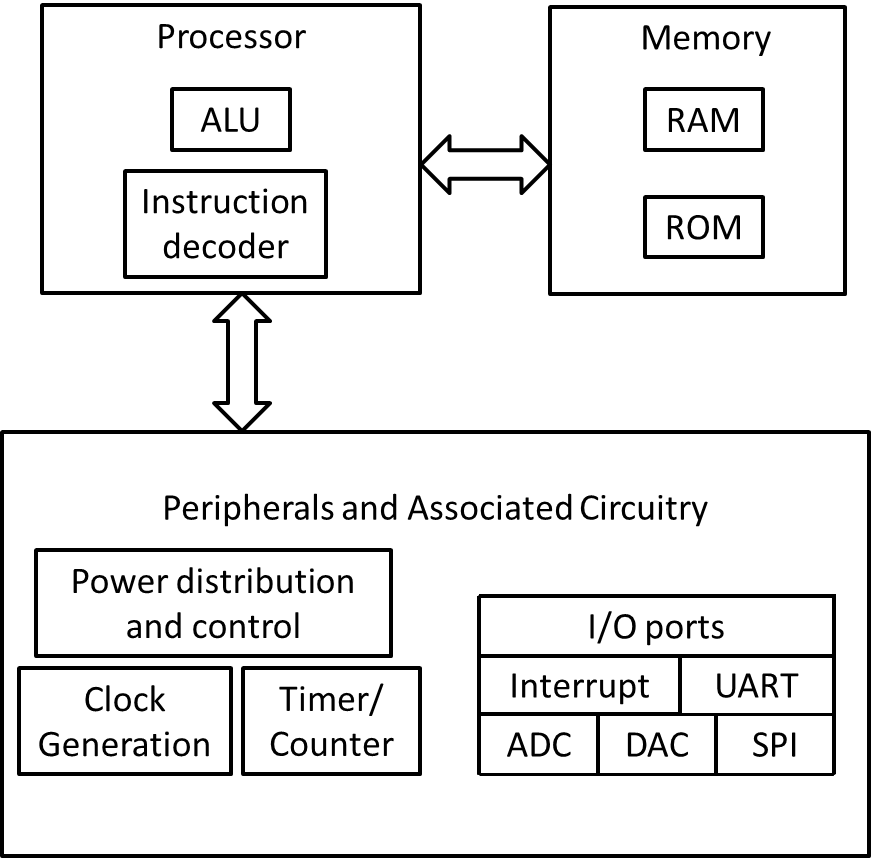
\includegraphics[width=\lgfig]{\LocHWfig/miccontblk.png}
  \caption{Functional block diagram of a microcontroller}
  \label{micro-arch}
\end{figure}

\begin{description}
  \item {Processor:} It is also known as a Central Processing Unit
        (CPU).  A processor is the heart of any computer/embedded
        system. The applications running on these systems involve arithmetic
        and logic operations. These operations are further simplified into
        instructions and fed to the processor.  The Instruction decoder
        decodes these instructions while arithmetic and logic operations are
        taken care of by an Arithmetic and Logic Unit (ALU). A modern day
        CPU can execute millions of instructions per second (MIPS).

  \item {Memory:}
        A computer memory, usually a semiconductor device, is used to hold data and instructions. Depending on the make, it could be volatile or non-volatile in nature. There are different types of memory:
        \begin{enumerate}
          \item Read Only Memory (ROM): It is a non-volatile storage entity. It
                is used in computers, phones, modems, watches and other electronic
                devices. A program is typically uploaded (flashed) to ROM through PC.
                Its content cannot be modified; it can only be erased and flashed
                using compatible tools.
          \item Random-access Memory: RAM is a volatile storage entity. It is
                used by CPU to store intermediate data during the execution of a
                program. RAM is usually faster than ROM.
          \item Electronically Erasable Programmable Read-Only Memory: EEPROM is
                an optional non-volatile storage entity. It can be erased and
                written by the running program.  For example, it can be used to
                store the values of a temperature sensor connected to the microcontroller.
        \end{enumerate}
\end{description}

\subsection{Microcontroller Peripherals}
Microcontrollers have a few built-in peripherals.  In this section, we
will review them briefly.

\begin{description}
  \item {Clock:} A complex digital circuit, such as the one that is
        present in a microcontroller, requires a clock pulse to
        synchronize different parts of it.  The clock
        is generated through internal or external crystal oscillator. A
        typical microcontroller can execute one instruction per clock
        cycle (time between two consecutive clock pulses).

  \item {Timer/Counter:} A timer is a pulse counter. A timer circuit is
        controlled by registers. An 8-bit timer can count from 0 to 255. A
        timer is primarily used to generate delay, and could be configured
        to count events.

  \item{Input/Output Ports:} I/O ports correspond to physical pins on
        the microcontroller. They are used to interface external peripherals. A
        port can be configured as input or output by setting bits in I/O
        registers. Each pin can be individually addressed too.

  \item{Interrupts:} An interrupt to the CPU suspends the running program
        and executes a code block corresponding to it. After serving/attending
        interrupts, the CPU resumes the previous program and continues. An
        interrupt could be originated by the software or the hardware. A
        hardware interrupt normally has a higher priority.

  \item {Universal Asynchronous Receiver/Transmitter (UART):} UART is a
        standard microcontroller peripheral to communicate with external
        serial enabled devices. It has two dedicated pins to be used as
        Rx (Receiver) and Tx (Transmitter).  The baud rate defines the speed
        of the UART and can be configured using registers.

  \item {Analog to Digital Converter (ADC):} Most of the signals around
        us are continuous. Digital circuits cannot process them. An ADC
        converts them into digital signals. The resolution of the ADC
        determines the efficiency of conversion. For example, a 10-bit
        resolution of the ADC relates to 1024 values per sample. This is
        shown pictorially in \figref{resolution}. Higher resolution relates
        to better translation of an analog signal.

        \begin{figure}
          \centering
          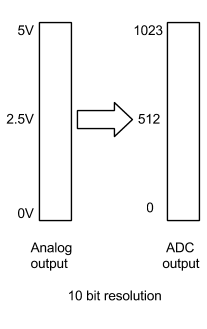
\includegraphics[width=\tnfig]{\LocHWfig/resolution.png}
          \caption{ADC resolution}
          \label{resolution}
        \end{figure}

  \item {Digital to Analog Converter (DAC):} Digital output of the CPU is
        converted to analog signals using the pulse width modulation (PWM)
        technique. The output of a DAC is used to drive analog devices and actuators.

  \item {Serial Peripheral Interface (SPI):} SPI is a synchronous 4 wire
        serial communication device. It requires a master and slave
        configuration. The SPI peripheral has dedicated pins and marked
        as:
        \begin{enumerate}
          \item SCLK (from Master)
          \item MOSI (Master out, Slave input)
          \item MISO (Master Input, Slave output)
          \item Slave select (Active when 0V, originates from Master)
        \end{enumerate}

  \item {Firmware:} Firmware is an application that configures the
        hardware. It is programmed to a non-volatile memory such as ROM,
        EPROM (Erasable Programmable ROM). This concept is used in computer
        BIOS and embedded devices.  In a microcontroller setup, a firmware
        file contains addresses and hexadecimal values.

  \item{Interfacing:} Some of the popular connections with microcontrollers include,
        \begin{enumerate}
          \item Digital input devices: Switch, keypad, encoder, multiplexer,
                touchscreen
          \item Digital output devices: LED, LCD, relay, buzzer
          \item Digital input and output devices: RTC (Real Time Clock),
                SD Card, external ROM
          \item Analog input devices: Audio, sensor, potentiometer
          \item Analog output devices: Brightness control, speaker
          \item Serial communication (UART): GSM, GPS, Zigbee, Bluetooth
        \end{enumerate}
\end{description}

\section{Open Source Hardware (OSHW)}
\label{sec:oshw}
In this section, we will introduce the reader to open source hardware
(OSHW), which is
\emph{defined} as follows \cite{oshw-ref}:
\begin{quote}
  Open source hardware is a hardware whose design is made publicly
  available so that anyone can study, modify, distribute, make, and sell
  the design or hardware based on that design...
\end{quote}
The OSHW website \cite{oshw-ref} gives additional conditions to be
fulfilled before the hardware can be called OSHW.  It also argues why
we should promote and contribute to OSHW.  The logo of OSHW is given
in \figref{fig:OSHW-logo} \cite{OSHW-logo-ref}.
\begin{figure}
  \centering
  
\includegraphics[width=1in]{\LocHWfig/OSHW-138px.png}
  \caption{The logo of Open Source Hardware}
  \label{fig:OSHW-logo}
\end{figure}
The open source hardware initiative is popular in the electronic,
computing hardware and automation industry.  Here are some examples of
open source hardware projects:
\begin{enumerate}
  \item The ``open compute project'' at Facebook shares the design of
        data center products.
  \item Beagle board, Panda board, OLinuXino are ARM based development
        boards.
  \item ``Open Graphics Project (OGP)'' releases the designs of
        graphics card.
  \item ``ArduCopter'' is a UAV (unmanned aerial vehicle) created by
        the \emph{DIY Drones} community.
  \item ``NetFPGA'' is a prototyping of computer network devices.
  \item ``OpenROV'' project (Open Source Remotely Operated Vehicle)
        aims at affordable underwater exploration.
  \item ``OpenMoko'' project set the foundation for open source mobile
        phones. ``Neo 1973'' was the first smartphone released in 2007
        with Linux based operating system, it had 128MB RAM and 64MB ROM.
\end{enumerate}

Companies like Adafruit Industries, Texas Instruments, Solarbotics,
Sparkfun electronics, MakerBot industries and DIY Drones have proven
the power of OSHW with their revenues.  Nevertheless, collaborative
innovation using OSHW is yet to establish itself in the mainstream.  But
the trend has certainly started and is going strong.  There are now
many robotics startups taking full use of OSHW.

\section {Arduino}
Arduino is an open source microcontroller board and a software
development environment. Arduino language is a \emph{C} like
programming language which is easy to learn and understand.  Arduino
has two components, open source hardware and open source software.  We
will cover the basics of the Arduino hardware in this section.

\subsection{Brief History}
Arduino project was started at the \emph{Interaction Design Institute
  Ivrea} in Ivrea, Italy. The aim was to create a low-cost
microcontroller board that anyone with little or no background domain
knowledge can design and develop. Arduino uses expansion circuit
boards known as \emph{shields}. Shields can provide GPS, GSM,
Bluetooth, Zigbee, motor and other functionality.

Within the first two years of its inception, the Arduino Team sold
more than 50,000 boards. In 2011, Google announced \emph{The Android
  Open Accessory Development Kit (ADK)}, which enables the Arduino boards to
interface with Android mobile platform.

Today Arduino is the first choice for electronic designers and
hobbyists. There are  more than 13 official variants of Arduino and
many more third-party Arduino software compatible boards.

\subsection{Arduino Uno Board}
There are different Arduino boards for different requirements. All
original Arduino boards are based on ATMEL microcontrollers.  In this
section, we will briefly discuss the \arduino\ board, the most popular
Arduino board.  We will illustrate all applications using the
\arduino\ board in this book.

Based on ATmega328, the \arduino\ board has 14 digital input/output
pins, 6 analog inputs, 6 PWM pins, a 16 MHz ceramic resonator, a power
jack, an ICSP (In-Circuit Serial Programming) header, and a reset
button. It has an on-board USB to serial converter and can be connected
to a PC using a USB cable. \figref{arduino} has a picture of this board
\cite{uno-ref}. \tabref{micro-table} has the specifications of the
\arduino\ board.

\begin{figure}
  \centering
  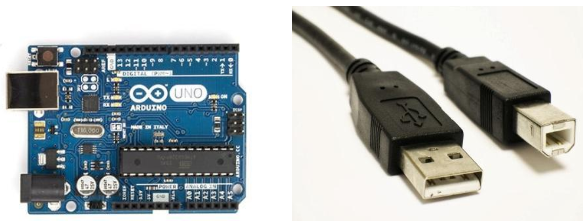
\includegraphics[width=\hgfig]{\LocHWfig/arduino.png}
  \caption{Arduino Uno Board}
  \label{arduino}
\end{figure}

\begin{table}
  \begin{center}
    \begin{tabular}{lc}
      \hline
      Parameter                   & Value                                        \\ \hline
      Microcontroller             & ATmega328P                                   \\
      Operating Voltage           & 5V                                           \\
      Input Voltage (recommended) & 7-12V                                        \\
      Input Voltage (limits)      & 6-20V                                        \\
      Digital I/O Pins            & 14 (of which 6 provide PWM output)           \\
      Analog Input Pins           & 6                                            \\
      DC Current per I/O Pin      & 20 mA                                        \\
      DC Current for 3.3V Pin     & 50 mA                                        \\
      Flash Memory                & 32 KB (ATmega328), 0.5 KB used by bootloader \\
      SRAM                        & 2 KB (ATmega328)                             \\
      EEPROM                      & 1 KB (ATmega328)                             \\
      Clock Speed                 & 16 MHz                                       \\
      Length                      & 68.6 mm                                      \\
      Width                       & 53.4 mm                                      \\
      Weight                      & 25 g                                         \\
      \hline
    \end{tabular}
    \caption{Arduino Uno hardware specifications}
    \label{micro-table}
  \end{center}
\end{table}

Another popular board is Arduino Mega board.  Based on
ATmega2560, this board has almost double the size of program
memory (ROM) compared to Arduino Uno.  It also has extra serial ports,
digital and PWM pins.  \figref{mega} has a picture of this board
\cite{mega-ref}.
\begin{figure}
  \centering
  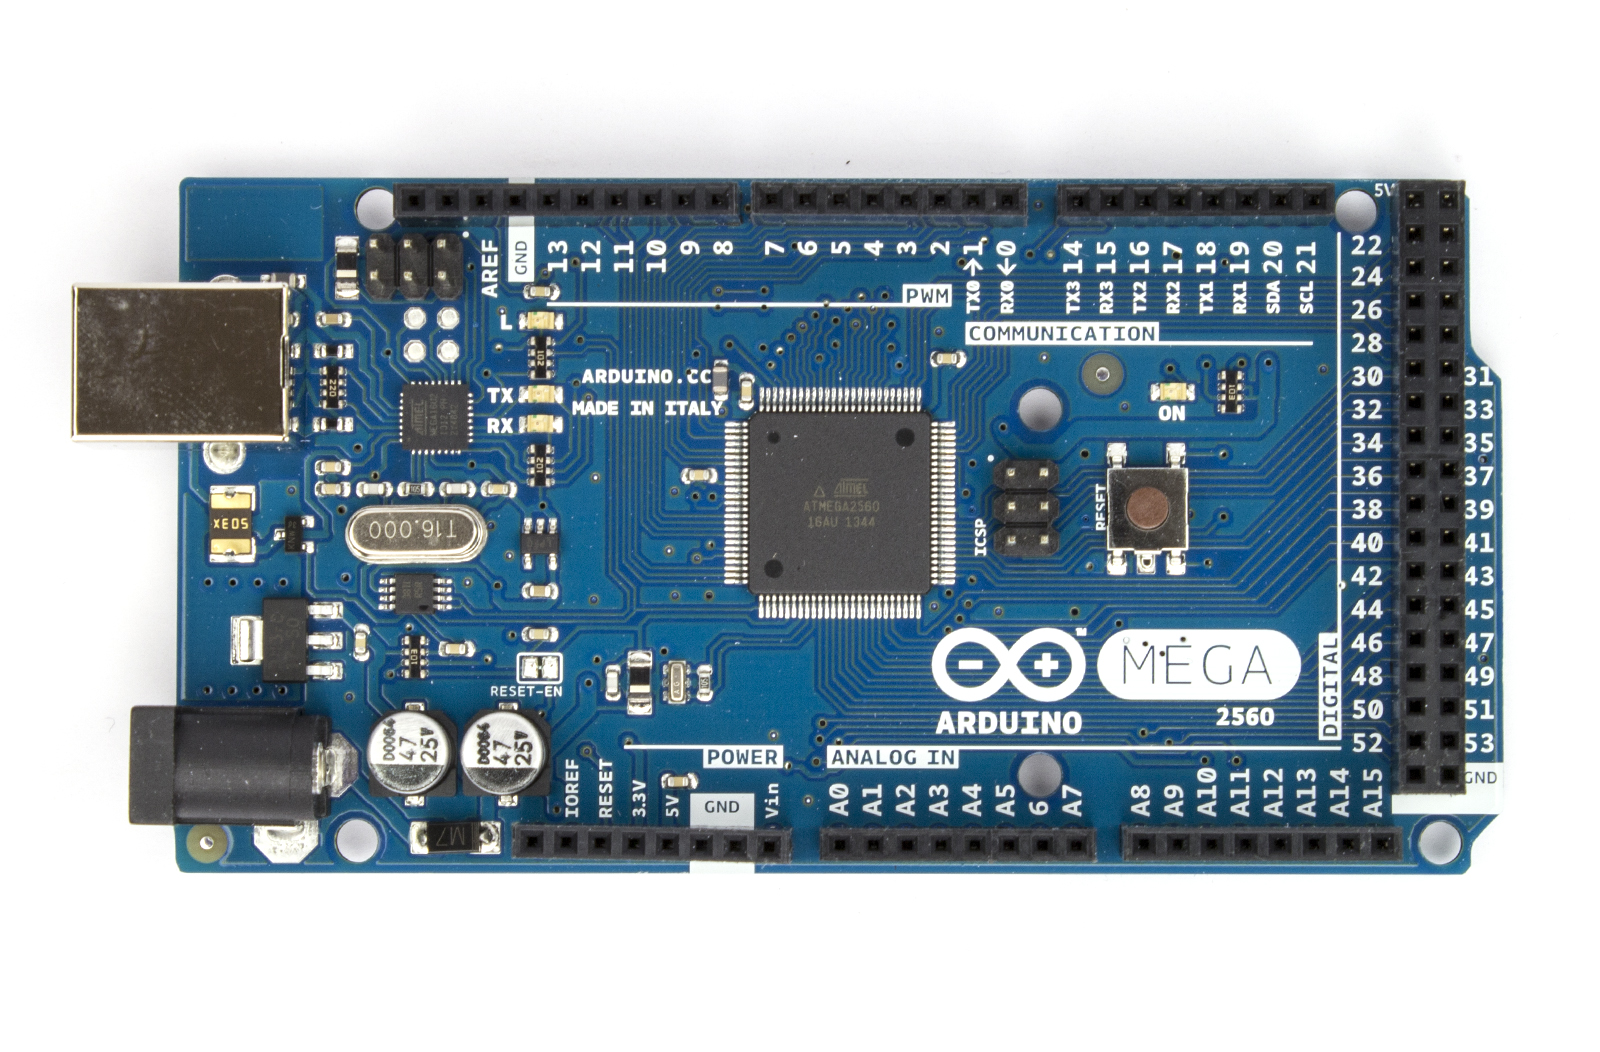
\includegraphics[width=\lgfig]{\LocHWfig/mega.jpg}
  \caption{Arduino Mega Board}
  \label{mega}
\end{figure}

Yet another popular board is LilyPad Arduino, a small circular
board for fabric designers. It can be stitched with conductive thread,
and it supports sensors and actuators.  \figref{lily} has a picture of
this board \cite{lily-ref}.
\begin{figure}
  \centering
  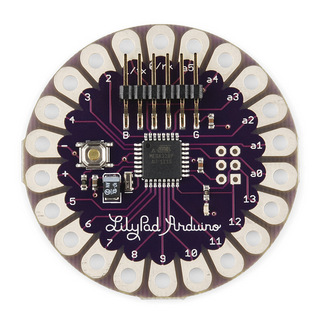
\includegraphics[width=\smfig]{\LocHWfig/lily.jpg}
  \caption{LilyPad Arduino Board}
  \label{lily}
\end{figure}

There are other similar configuration boards with different form
factors, such as Arduino Fio, Arduino Mini, Arduino Nano, Arduino
Duemilanove, Arduino serial and so on.

\subsection{Popular Arduino Projects}
Arduino is intuitive and it's easy to setup and use. That's why people around the globe
are using Arduino in innovative ways. We list a few of these projects to give a
flavor of some of these interesting applications.

\paragraph{Arduino phone:} An Arduino connected with a graphic LCD and a
GSM shield. This low-tech phone, shown in \figref{arduino-phone} can
be built in a few hours \cite{phone-ref}.
\begin{figure}
  \centering
  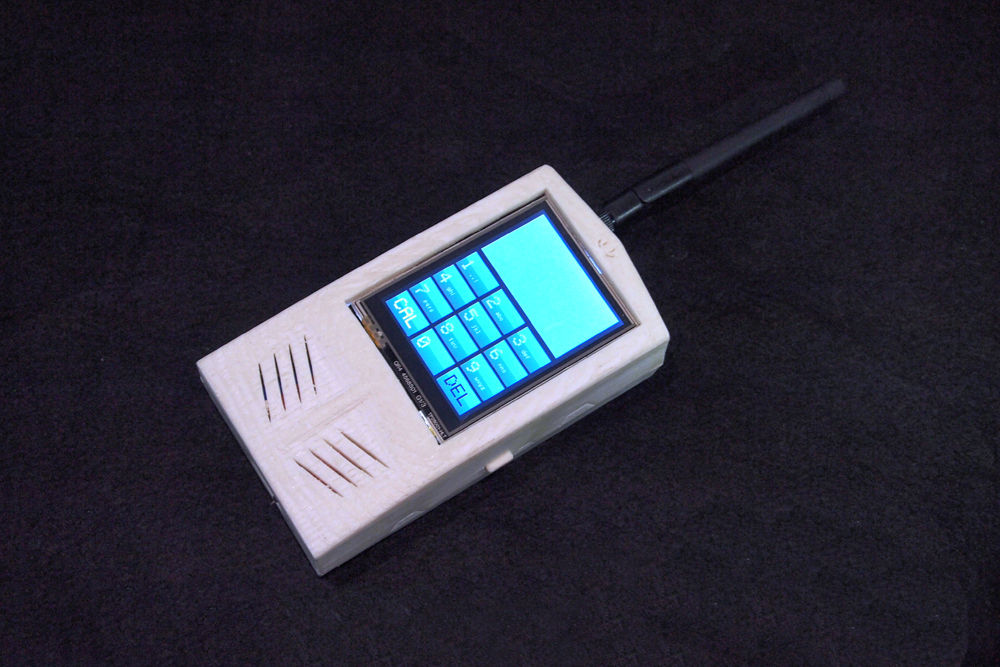
\includegraphics[width=\smfig]{\LocHWfig/arduino-phone.jpg}
  \caption{Arduino Phone}
  \label{arduino-phone}
\end{figure}

\paragraph{Candy sorting machine:} As the name suggests, this machine
can sort candy based on its color to separate jars \cite{candy-ref}.

\paragraph{3D printers:} There are open source 3D printers based on
Arduino and  Raspberry Pi. Although 3D printers, shown in \figref{3dprinter},
are relatively slow and lack precision, they can be ideal for building prototypes by
hobbyists \cite{3d-printer-ref}.
\begin{figure}
  \centering
  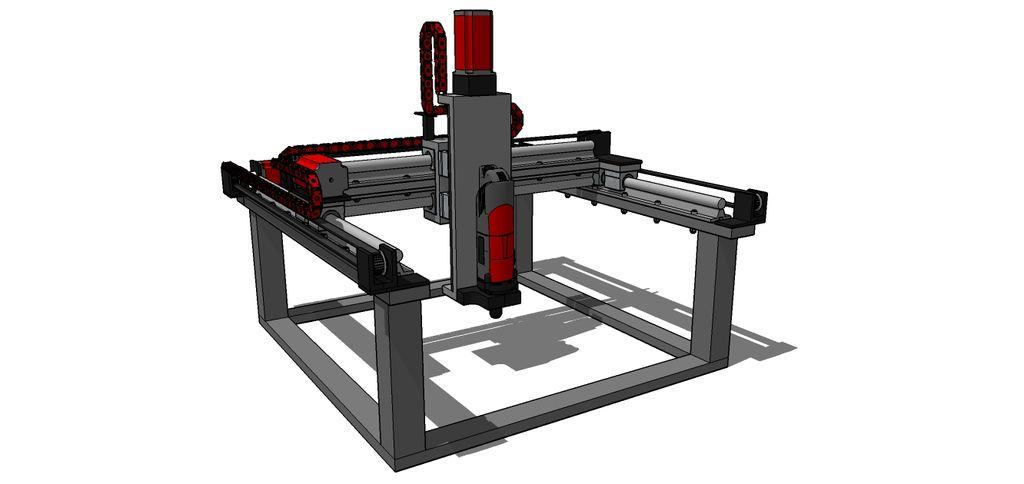
\includegraphics[width=\smfig]{\LocHWfig/arduino-3d-printer.jpg}
  \caption{3D printer}
  \label{3dprinter}
\end{figure}

\section{Shield}\label{shield-hw}
The Shield that we use in this book is a modified version of the Diyode Codeshield
board \cite{shield-ref}, which makes it easy to perform
experiments on the \arduino\ board.  The Shield is a printed circuit
board (PCB) with a large number of sensors, already wired and hence,
ready to use.  It obviates the need for a breadboard as an
intermediate tool for electronics circuit prototyping, which is quite
cumbersome for beginners.  The Shield provides the user a faster way
of circuit prototyping without worrying much about troubleshooting.

The numbering on the Shield is identical to that on
the \arduino\ board.  The Shield fits snugly on to the \arduino\
board, obviating the need to do the wiring in many experiments.  One
can even say that Shields have made the hardware experiments involving
Arduino boards as easy as writing software.

All the experiments in this book have been verified with the use of a
modified version of Diyode Codeshield, as mentioned above.  We make
available all the required information to make a Shield, thus making
this an OSHW, see \secref{sec:oshw}.

We now explain where the required files to make our Shield are given.
The gerber file to make the Shield is given in
\LocSHbrief{gerber-V1.2}. The image of the PCB file is given in
\figref{fig:PCB-image}. The PCB project files are available in a
folder at \LocSHbrief{kicad-import}.
\begin{figure}
  \centering
  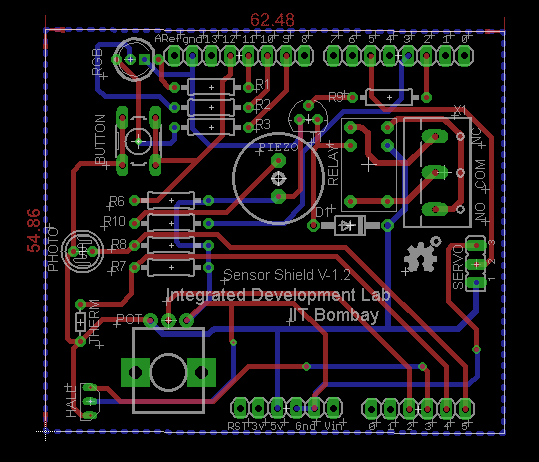
\includegraphics[width=\lgfig]{\LocSH/pcb_board_V1p2.png}
  \caption[PCB image of the Shield]{PCB image of the Shield}
  % The PCB file can be found at \LocSHbrief{shield-V1p2.brd}.
  \label{fig:PCB-image}
\end{figure}
The pictorial representation of the schematic for the Shield is given
in \figref{fig:sch-shield}.
\begin{figure}
  \centering
  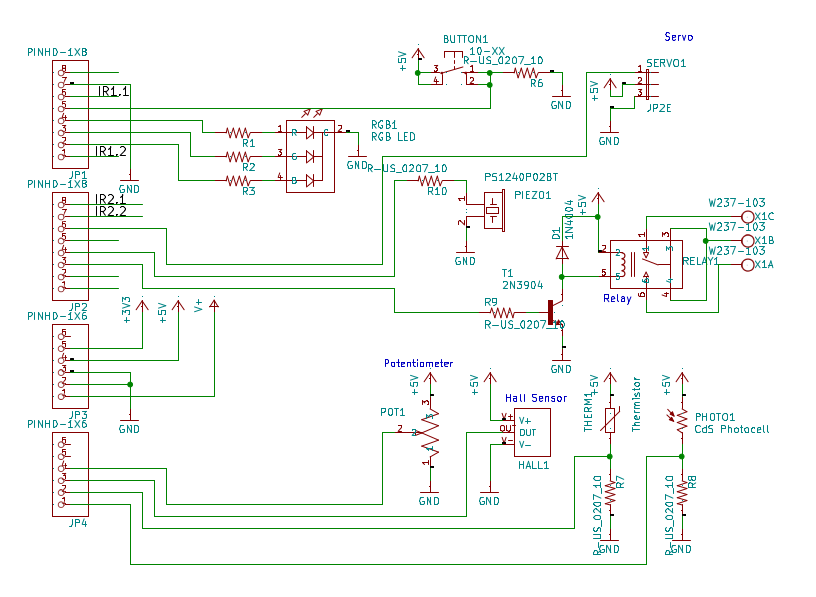
\includegraphics[width=\linewidth]{\LocSH/shield-V1p2.png}
  \caption{Pictorial representation of the schematic of the Shield}
  \label{fig:sch-shield}
\end{figure}
A photograph of the PCB after fabrication is given in
\figref{fig:shield-photo}.

\begin{figure}
  \centering
  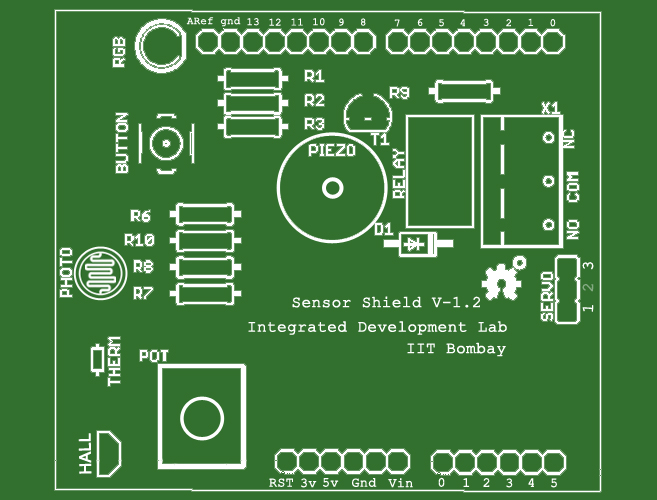
\includegraphics[width=0.6\linewidth]{\LocSH/shield-V1p2.jpg}
  \caption{PCB of the Shield}
  \label{fig:shield-photo}
\end{figure}
The values of the various components used in the Shield are given in
\tabref{tab:shield-values}.
\begin{table}
  \centering
  \caption{Values of components used in the Shield}
  \label{tab:shield-values}
  \begin{tabular}{llc} \hline
    Name       & Description                     & Quantity \\ \hline
    R1, R10    & $100\Omega$ Resistor (Br-Bl-Br) & 2        \\
    R2, R3     & $91\Omega$ Resistor (Wt-Br-Bl)  & 2        \\
    R6, R7, R8 & $10K\Omega$ Resistor (Br-Bl-Or) & 3        \\
    R9         & $1K\Omega$ Resistor (Br-Bl-Rd)  & 1        \\
    D1         & Diode                           & 1        \\
    Relay      & Relay                           & 1        \\
    X1         & Terminal block                  & 1        \\
    Piezo      & Buzzer                          & 1        \\
    % LED 1          & LED - 2 lead                    & 1        \\
    RGB        & RGB LED                         & 1        \\
    T1         & Transistor                      & 1        \\
    % SWITCH         & Switch                          & 1        \\
    BUTTON     & Pushbutton                      & 1        \\
    PHOTO      & Light dependent resistor        & 1        \\
    HALL       & Hall effect sensor              & 1        \\
    POT        & Potentiometer                   & 1        \\
    % ENC & Rotary encoder & 1 \\
    THERM      & Thermistor                      & 1        \\
    SERVO      & Servomotor                      & 1        \\
    % SERVO-PARTS    & Servo parts                     & 1        \\
    % NUT, BOLT & Nut, bolt & 2 \\
    HEADER     & 6x pin header                   & 2        \\
    HEADER     & 8x pin header                   & 2        \\
    \hline
  \end{tabular}
\end{table}
\tabref{shield-table} provides information about various sensors,
components on Shield and its corresponding pin on \arduino\ board
\cite{shield-ref}.
\begin{table}
  \centering
  \caption{Information on sensors and pin numbers}
  \label{shield-table}
  \begin{tabular}{llc}
    \hline
    Shield components   & Arduino pin    \\ \hline
    RELAY               & Digital pin 2  \\
    BUZZER              & Digital pin 3  \\
    SERVO               & Digital pin 5  \\
    RGB LED BLUE        & Digital pin 9  \\
    RGB LED GREEN       & Digital pin 10 \\
    RGB LED RED         & Digital pin 11 \\
    PUSHBUTTON          & Digital pin 12 \\
    POTENTIOMETER       & Analog pin 2   \\
    HALL EFFECT SENSOR  & Analog pin 3   \\
    THERMISTOR          & Analog pin 4   \\
    PHOTORESISTOR (LDR) & Analog pin 5   \\

    \hline
  \end{tabular}
\end{table}
A picture of the completed Shield is in \figref{shield}. The information on purchasing this Shield is given in Appendix \ref{shield-appendix}.
\begin{figure}
  \centering
  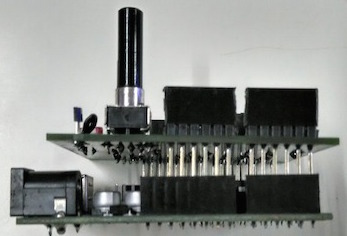
\includegraphics[width=\linewidth]{\LocHWfig/shield-crop.jpg}
  \caption{Picture of the Shield with all components}
  \label{shield}
\end{figure}

\section{Experimental Test Bed}
We experimented with the contents of this book with the
following list.  We will refer to this as a \emph{kit} in the rest of
this book.
\begin{enumerate}
  \item \arduino\ board
  \item Shield containing
        \begin{enumerate}
          \item LED
          \item LDR
          \item Push Button
          \item Thermistor
        \end{enumerate}
  \item DC motor and its controller board
  \item Servomotor
  \item Energy meter with Modbus interface
\end{enumerate}

The \arduino\ board is easily available in the market.  The Shield is
designed by us.  Details of most of these units are provided in the
previous sections.  Information on all of these is available in the
file, mentioned in \fnref{fn:file-loc}, and in the Appendix.

\section{Doing the Experiments with a Breadboard}
\label{sec:hw-bread}
It is possible to carry out many of the experiments listed in this
book using a breadboard.  For example, carrying out experiments with
an LED is explained in Sec.~\ref{sec:led-bread}.  To carry out all the
experiments using a breadboard, as explained in the subsequent
chapters, one needs the components listed in
Table~\ref{tab:bread-comps}.  

\begin{table}
  \centering
  \caption{Lists of components to work with the breadboard}
  \label{tab:bread-comps}
  \begin{tabular}{lc}
    \hline
    Components                & Quantity \\ \hline
    \arduino\ with USB cable  & 1        \\
    Half breadboard           & 1        \\
    Male to Male jumper wires & 10       \\
    $100\Omega$ Resistor      & 5        \\
    $10K\Omega$ Resistor      & 2        \\
    RGB LED                   & 1        \\
    Pushbutton                & 1        \\
    Photoresistor (LDR)       & 1        \\
    Potentiometer             & 1        \\
    Thermistor                & 1        \\
    Buzzer                    & 1        \\
    Servomotor                & 1        \\
    L293D motor driver board  & 1        \\
    DC motor                  & 1        \\
    \hline
  \end{tabular}
\end{table} 

% \chapter{Communication between Software and Arduino}
\thispagestyle{empty}
\label{sec:sw-env}

\newcommand{\LocSWfig}{\Origin/user-code/sw-env/figures}
\newcommand{\LocSWscicode}{\Origin/user-code/sw-env/scilab}
\newcommand{\LocSWscibrief}[1]{{\texttt
                  Origin/user-code/sw-env/scilab/#1}, see \fnrefp{fn:file-loc}}
\newcommand{\LocSWardcode}{\Origin/user-code/sw-env/arduino}
\newcommand{\LocSWardbrief}[1]{{\tt \seqsplit{
                        Origin/user-code/sw-env/arduino/#1}}, see \fnrefp{fn:file-loc}}

\newcommand{\LocSWchkcode}{\Origin/tools/scilab}
\newcommand{\LocSWchkbrief}[1]{{\tt \seqsplit{
                        Origin/tools/scilab/#1}}, see \fnrefp{fn:file-loc}}
\newcommand{\LocSWfirmcode}{\Origin/tools/floss-firmware}
\newcommand{\LocSWfirmbrief}[1]{{\tt \seqsplit{
                        Origin/tools/floss-firmware/#1}}, see \fnrefp{fn:file-loc}}

\newcommand{\LocFIMpycode}{\Origin/tools/python}  %added for python
\newcommand{\LocFIMpybrief}[1]{{\tt \seqsplit{%
                        Origin/tools/python/#1}}, see \fnrefp{fn:file-loc}} % added for python


\newcommand{\LocFIMjuliacode}{\Origin/tools/julia}  %added for julia
\newcommand{\LocFIMjuliabrief}[1]{{\tt \seqsplit{%
                        Origin/tools/julia/#1}}, see \fnrefp{fn:file-loc}} % added for julia

%%%%%%OpenModelica Starts
\newcommand{\LocFIMOpenModelicacode}{\Origin/tools/openmodelica/windows/}  %added for OpenModelica
\newcommand{\LocFIMOpenModelicabrief}[1]{{\tt \seqsplit{%
                        Origin/tools/openmodelica/windows/#1}}, see \fnrefp{fn:file-loc}} % added for OpenModelica

%%%%%OpenModelica Ends


In this chapter, we shall briefly walk through the software
environment that needs to be set up before we could start with the
\arduino\ board-based experiments. We shall start with the \arduino\
compatible Integrated Development Environment (IDE), termed as Arduino
IDE, that would be used to load the FLOSS firmware on to the
microcontroller. The FLOSS firmware to be loaded could be developed to serve
different purposes as per the requirement. For example, 
\begin{itemize}
      \item To run \arduino\ stand-alone, without waiting for any commands
            from other software or hardware, for the specified time or until
            power off
      \item To decode the commands sent by other software, such as Scilab, Python, 
            Julia, OpenModelica, etc., through a serial port, and 
            execute the given instructions %\item Combination of the above two
\end{itemize}
Next, we shall discuss Scilab and Xcos, which are open-source software
tools, and a related toolbox that can communicate with \arduino\ 
over a serial port using RS232 protocol. Subsequently, we shall discuss 
other open-source software tools such as Python, Julia, and OpenModelica. 

\section{Arduino IDE}\label{arduino-ide}
\label{sec:ard-start}
Arduino development environment is compatible with popular desktop
operating systems. In this section, we will learn to set up this tool
for the computers running Microsoft Windows or Linux. Later, we shall
explore the important menu options in the Arduino IDE and run a sample
program.  The following two steps have to be followed whatever operating
system is used:

\begin{enumerate}
      \item To begin, we need an \arduino\ board with a USB cable (A plug to
            B plug) as shown in \figref{arduino}.
      \item Connect it to a computer and power it up. The moment you connect \arduino\
            to the computer, an on-board power LED will turn ON.
\end{enumerate}

\subsection{Downloading and installing on Windows}
First, carry out the steps numbered 1 and 2 given above.
Starting from download, we shall go through the steps to set up
Arduino IDE on Windows OS:

\begin{enumerate}
      \setcounter{enumi}2
      \item Visit the URL, {\tt https://www.arduino.cc/en/software}. On the 
            right right side of the page, locate the link \emph{Windows ZIP file} and click on it.  
            This may redirect you to the download/donate page. Read the instructions and proceed with the
            download.
      \item Extract the downloaded ZIP file to Desktop. Do not alter any
            file or directory structure.
      \item Click on the Windows Start Menu, and open up the ``Control
            Panel''.
      \item While in the Control Panel, navigate to ``System and Security'',
            click on ``System'' and then choose the ``Device Manager''.
      \item Look for ``Other devices'' in the ``Device Manager'' list,
            expand and locate ``Unknown device''.  This may be similar to what
            is shown in \figref{win-device-manager}. In case, you don't see  
            ``Unknown device,'' look for ``Ports (COM \& LPT)'' and expand it to locate 
            ``USB Serial Device (COM2)''.
            This may be similar to what is shown in \figref{win-device-manager-com}.
      \item Right-click on the ``Unknown device'' (or ``USB Serial Device (COM2)'' as shown in 
            the previous step) and select the ``Update Driver Software'' (or ``Update driver'') option 
            as shown in \figref{win-dri-update}. 
      \item Next, choose the ``Browse my computer for Driver software''
            option.
      \item Navigate to the newly extracted Arduino folder on the Desktop and
            select ``drivers'' folder.
      \item Windows will now finish the driver installation. The Arduino IDE
            is ready for use.
\end{enumerate}
To launch Arduino IDE, browse to extracted Arduino folder on the Desktop and double click on ``arduino.exe''.
\begin{figure}
      \centering
      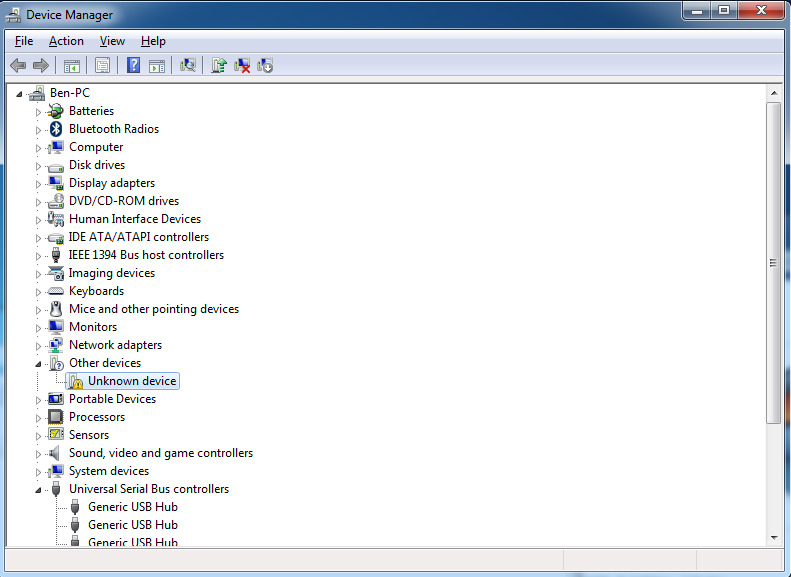
\includegraphics[width=\linewidth]{\LocHWfig/hw-device-manager.jpg}
      \caption{Windows device manager}
      \label{win-device-manager}
\end{figure}

\begin{figure}
      \centering
      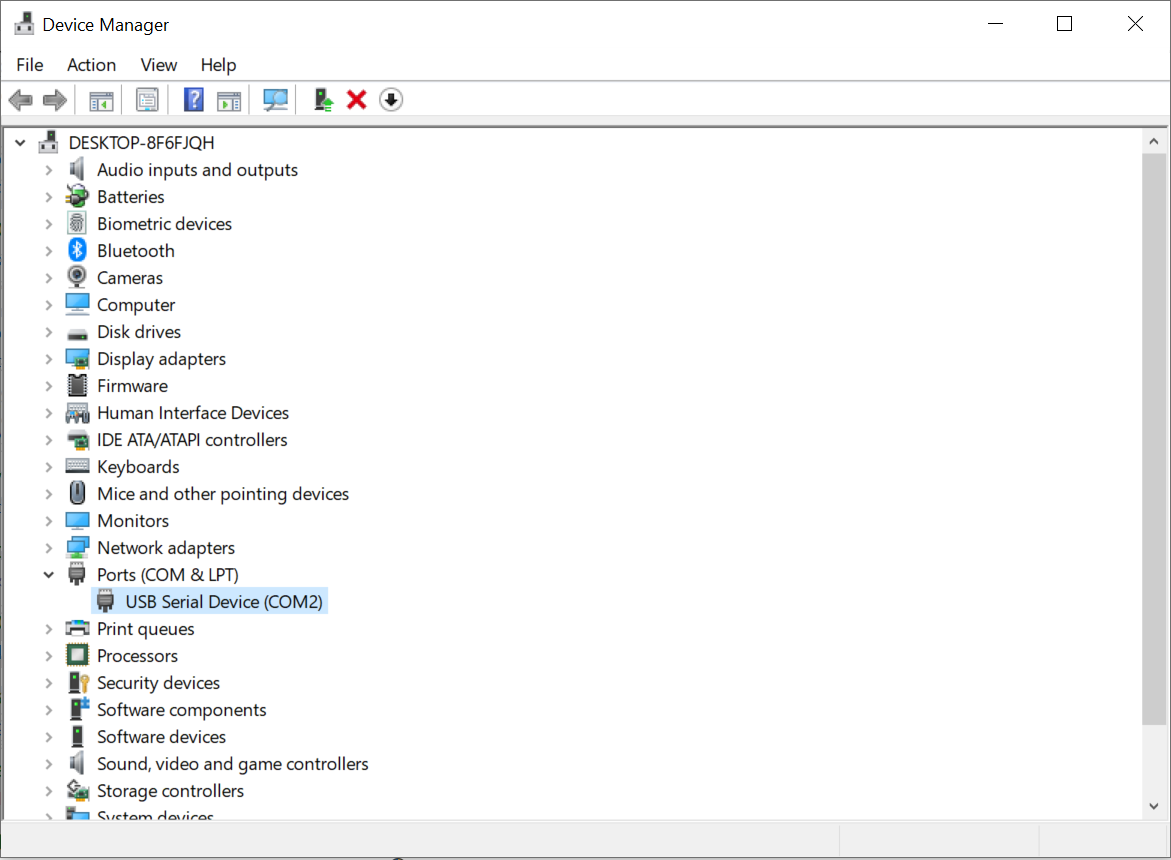
\includegraphics[width=\linewidth]{\LocSWfig/device-manager-com.png}
      \caption{Windows device manager}
      \label{win-device-manager-com}
\end{figure}

\begin{figure}
      \centering
      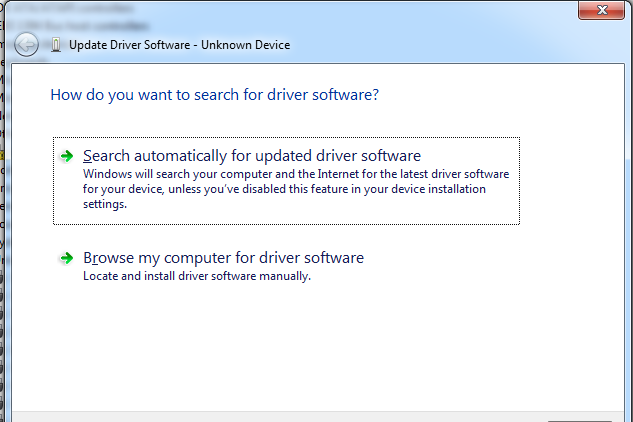
\includegraphics[width=\linewidth]{\LocHWfig/update-driver.png}
      \caption{Windows update driver option}
      \label{win-dri-update}
\end{figure}


\subsection{Downloading and installing on GNU/Linux Ubuntu}
We will now explain the installation of Arduino software on the
GNU/Linux operating system. We shall perform the installation on the 64-bit 
Ubuntu 18.04 LTS operating system.  These
instructions will work for other GNU distributions too, with little or
no modification.  First, carry out the steps numbered 1 and 2 given
above.  Then carry out the following:

\begin{enumerate}
      \setcounter{enumi}2
      \item First, update your system. Open the terminal emulator, type,
            {\tt sudo apt-get update} and press Enter. 
      \item Find out your operating system support for 64-bit
            instructions. Open the terminal emulator and type, {\tt uname -m}
      \item If it returns ``x86\_64'', then your computer has 64-bit
            operating system.   There is no visible performance difference in 32
            and 64-bit Arduino versions.
      \item Download the suitable Arduino Software version (32 or 64-bit)
            from \\ {\tt https://www.arduino.cc/en/software}.  As mentioned
            earlier, we will perform experiments with a 64-bit installation.
            
      \item At the time of writing this book, we worked with version 1.8.13.
            Assuming that you have downloaded the tar file in 
            the Downloads directory, execute the following
            commands on the terminal:
            \begin{quote}
                  {\tt cd {\large\textasciitilde}/Downloads\\
                        tar -xvf arduino-1.8.13-linux64.tar.xz\\
                        sudo mv arduino-1.8.13 /opt}
            \end{quote}
            
      \item In the same terminal session, install the required Java Runtime
            Environment with a command like,
            {\tt sudo apt-get -y install openjdk-8-jre}
            
      \item \label{itm:port-check} Execute the
            following command on the terminal to list the serial port number.\\
            {\tt ls /dev/ttyACM*}\\
            Note down the serial device filename.  Suppose that it
            is {\tt ttyACM0}.
      \item \label{itm:port-access} To make the USB port available to all users, set the read-write
            permission to the listed port:
            {\tt sudo chmod a+rw /dev/ttyACM0}. Each time you plug the \arduino\
            into the computer, you need to execute the commands given in the steps 
            numbered \ref{itm:port-check} and \ref{itm:port-access}. 
            
      % \item \label{itm:create-shortcut} Create a shortcut on the desktop:\\
      %       {\tt cd {\large \textasciitilde}/Desktop\\
      %       ln -s /opt/arduino-1.8.13/arduino}
      % \item \label{itm:give-permission} Give executable permission to this file through the following
      %       command on the terminal: {\tt chmod +x arduino}
            %   Ubuntu opens executable text files with an editor instead of
            %   executing them. To be able execute a file, open the ``Files''
            %   program from the launcher, go to menu ``Edit'', ``Preferences'', tab
            %   ``Behavior'' and set ``Executable Text Files'' to ``Ask each time'',
            %   as shown in \figref{ard-lin-executable}.
            
\end{enumerate}
% \begin{figure}
%   \centering
%   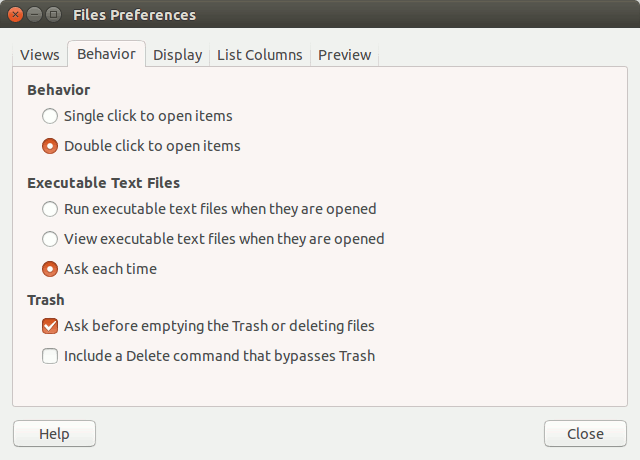
\includegraphics[scale=0.5]{\LocHWfig/executable.png}
%   \caption{Executable permission to Arduino IDE}
%   \label{ard-lin-executable}
% \end{figure}
% Then double click the Arduino shortcut on the Desktop and, click ``Run''
% in the dialog window to start the Arduino IDE. The dialog box is shown in \figref{ard-lin-run} for reference.
% \begin{figure}
%       \centering
%       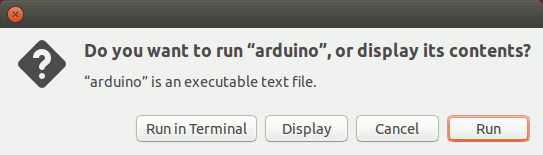
\includegraphics[scale=0.5]{\LocHWfig/run.png}
%       \caption{Confirmation for executing Arduino script}
%       \label{ard-lin-run}
% \end{figure}
The Arduino IDE is now ready for use. To launch it, carry out the steps given below:
\begin{enumerate}
      \item Open a terminal by pressing the Alt+Ctrl+T keys together.
      \item Navigate into the {\tt opt} directory, as shown in \figref{arduino-opt}.\\
      {\tt cd /opt/arduino-1.8.13/}
      \item Start the Arduino IDE by executing the command {\tt ./arduino}
\end{enumerate}


% There are chances that you might not 
% get the Arduino shortcut on your Desktop after executing the commands given in 
% steps numbered \ref{itm:create-shortcut} and \ref{itm:give-permission}. 
% In that case, you can navigate into the {\tt /opt/} directory and execute the 
% commands as given in \figref{arduino-opt} to start the Arduino IDE. 

\begin{figure}
      \centering
      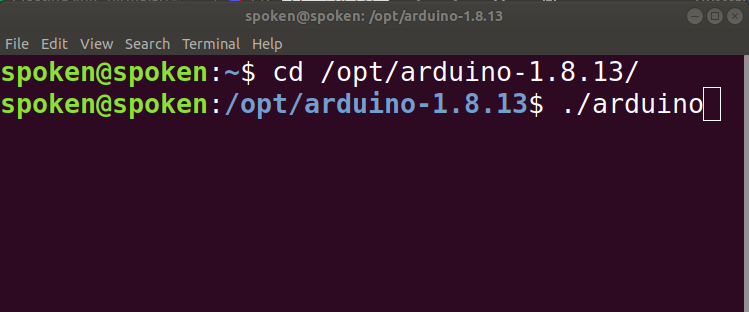
\includegraphics[width=\lgfig]{\LocSWfig/launch-arduino-opt.png}
      \caption{Linux terminal to launch Arduino IDE}
      \label{arduino-opt}
\end{figure}


\subsection{Arduino Development Environment}
\label{sec:Arduino-IDE}
The Arduino development environment, as shown in \figref{ard-ide},
consists of 
a text editor for writing code, a message area, a text console, a
toolbar with buttons for common functions, and a series of menus. It
connects to the Arduino hardware to upload programs and communicate
with them.

\begin{figure}
      \centering
      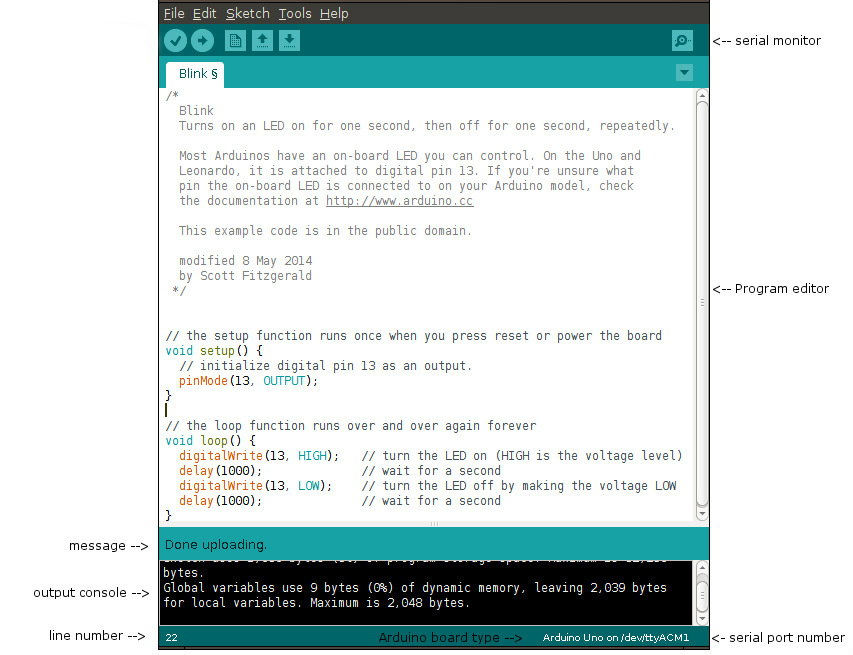
\includegraphics[width=\linewidth]{\LocHWfig/arduino-ide.jpg}
      \caption{Arduino IDE}
      \label{ard-ide}
\end{figure}
Software written using Arduino is called sketches. These sketches are
written in the text editor. Sketches are saved with the file extension
``.ino''. The frequently used icons shown in the toolbar, below the menu bar, are explained next. The names of these icons can be viewed by hovering the mouse pointer over each of them.

\begin{enumerate}
      \item Verify: Checks your code for errors
      \item Upload: Compiles your code and uploads it to the Arduino I/O
            board
      \item New: Creates a new sketch
      \item Open: Presents a menu of all the sketches in your
            sketchbook - clicking one will open it within the current window
      \item Save: Saves your sketch
      \item Serial Monitor: Opens the serial port window - the location of
            this is shown in the top right-hand corner of \figref{ard-ide}
\end{enumerate}
Note that these appear from left to right in the editor window. Next, we shall go through the additional useful options under the menu.
\begin{enumerate}
      \item File
            \begin{enumerate}
                  \item Examples: Examples that come at the time of installation
                  \item Page Setup: Configures the page parameters for the printer
                  \item Preferences: Customizes font, language, and other parameters for
                        the IDE
            \end{enumerate}
      \item Sketch
            \begin{enumerate}
                  \item Include Library: Adds a library to your sketch by inserting {\tt
                                    \#include} statements at the start of your code
            \end{enumerate}
      \item Tools
            \begin{enumerate}
                  \item Auto Format: Indents code so that opening and closing curly
                        braces line up
                  \item Archive Sketch: Archives a copy of the current sketch in .zip
                        format. The archive is placed in the same directory as the sketch.
                  \item Board: Selects the board that you're using
                  \item Port: This menu contains all the serial devices (real or
                        virtual) on your machine. It should automatically refresh every time
                        you open the top-level tools menu.
                  \item Programmer: This can be used to select a hardware programmer when programming a board or chip and not using the onboard USB-serial
                        connection. Normally you won't need this, but if you're burning a
                        bootloader to a new microcontroller, you will use this.
                  \item Burn Bootloader: The items in this menu allow you to burn a
                        bootloader onto the microcontroller on an Arduino board. This is not
                        required for normal use of an Arduino board but is useful if you
                        purchase a new ATmega microcontroller (which normally comes without a
                        bootloader). Ensure that you've selected the correct board from the
                        Boards menu before burning the bootloader.
            \end{enumerate}
\end{enumerate}

\subsection{Testing Arduino with a sample program}
\label{sec:testing-arduino}
Now, as we have a basic understanding of Arduino IDE, let us try an
example program.
\begin{enumerate}
      \item Open the Arduino IDE by clicking the shortcut ``arduino'' from
            Desktop in Ubuntu. In MS Windows browse to extracted Arduino folder
            on Desktop and double click on ``arduino.exe''.
      \item In the Arduino IDE, to know the path of your sketch files,
            navigate to File, then Preferences and then locate the ``Sketchbook
            location'' text box at the top.  You may change the path of your
            storage location. In this book, we will keep it unchanged. The path
            will be different for Windows and Ubuntu.
      \item To load a sample program, navigate and click on sketch ``File'',
            then Examples, then 01.Basics, and then Blink.
      \item A new IDE instance will open with Blink LED code.  You may close
            the previous IDE window now.
      \item Click ``verify'' to compile. The ``status bar'' below the text editor
            shall show ``Done compiling'' on success.
      \item Connect Arduino UNO board to PC. You may connect the board
            before writing the sketch too.
      \item Now, navigate to ``Tools'', then Port, and select the available
            port. If the port option is greyed out (or disabled) then reinsert the
            USB cable to the PC.
      \item Now select the upload button to compile and send the firmware to
            the Arduino Uno board.
      \item If the upload is successful, you will notice the onboard orange LED
            next to the Arduino logo will start blinking.
      \item It is safe to detach the USB cable at any moment.
\end{enumerate}

Arduino programming syntax is different from other languages. In an
embedded setup, a program is expected to run forever. To facilitate
this, the Arduino programming structure has two main functions: {\tt setup()}:
Used to initialize variables, pin modes, libraries, etc. The setup
function will run only once after each powerup or board reset.
{\tt loop()}: Code inside this function runs forever. An Arduino program
must have {\tt setup()} and {\tt loop()} functions.  We will give several examples
in this book to explain this usage.

An inbuilt offline help is available within the IDE. You may access
the explanation on IDE by navigating to ``Help'' and then
Environment.

\subsection{FLOSS Firmware}
We have provided a code to check whether the FLOSS firmware has been
properly installed.  The first few lines of this code follow. 

\begin{ardcode}
      \acaption{First 10 lines of the FLOSS firmware}{First 10 lines of
            the FLOSS firmware.  Available at
            \LocSWfirmbrief{floss-firmware.ino}. Following the
            steps given in sections \ref{sec:Arduino-IDE} and 
            \ref{sec:testing-arduino}, open this code in 
            Arduino IDE and upload it to \arduino. 
            Once the upload is successful, you should expect a success message 
            at the bottom of Arduino IDE, as shown in \figref{ard-ide}. }
      \label{ard:firmware}
      \lstinputlisting[firstline=1,lastline=10]
      {\LocSWfirmcode/floss-firmware.ino}
\end{ardcode}

% \subsection{Arduino firmware to work with scilab toolbox}
% \label{sec:firmware}
% A firmware is basically a program that continuously runs inside a
% microcontroller. It is a collection of routines corresponding to the
% required functionalities. It is typically written in Assembly and C
% programming language. It is compiled and converted into
% binary(hexadecimal values with addresses) for the target
% microcontroller. The binary file(also called hex file) is then
% uploaded to the microcontroller’s internal ROM. The firmware that has to
% be used to work with scilab toolbox is at \ardref{ard:firmware}.  It
% is an Arduino IDE compatible file and can be opened in an Arduino
% IDE. Let us see a brief explanation of this firmware.

% The firmware used for Arduino Uno in this book has the following tasks
% to perform:
% \begin{enumerate}
% \item Reading instructions from a computer(running Scilab) over serial
%   interface and decoding them. 
% \item Performing the task mentioned in the instruction.
% \item Optionally sending data back to the computer over an serial
%   interface.
% \end{enumerate}
% Let us see a simple example of reading values from the LDR that is
% on the shield.

% The firmware waits for a particular character (command) to be sent
% from the computer. The character “A”, in quoted form, as shown here,
% is reserved for analog read
% routine. So if Scilab wants analog values from the microcontroller, it
% sends the character “A” to Arduino Uno. On receiving “A”, the Arduino
% Uno 
% jumps to the routine of Analog read. Here it again waits for the
% computer to now send the pin number from where it is supposed to read
% the LDR value. This pin number is in ASCII text. Arduino Uno first
% checks if the ASCII lies between a valid range. If yes, it takes its
% ASCII value as a valid pin number. The value 48 is subtracted from it
% to reveal the character and thus the pin number. This pin number is
% then sent to the analogRead() function. The analogRead() function is
% an inbuilt Arduino function imported from the header file. The
% analogRead() function then actually reads from the pin and returns the
% analog value. This value is then sent back to the
% computer(Scilab). The correct firmware must be loaded inside Arduino
% Uno to be able to successfully carry out any of the experiment
% explained throughout this book. It is strongly recommended to confirm
% this before proceeding. 

\section{Scilab}
\label{sec:sci-start}
Scilab is a free and open-source computing software for science and
engineering applications \cite{scilab-ref}. It is released under GPL
compatible CeCILL license.  It uses the state-of-the-art linear
algebra package LAPACK, just as in Matlab.  Scilab has hundreds of
inbuilt functions which cater to a variety of areas such as signal
processing, control system design, statistics, optimization, and many
more. It has 2D and 3D visualisation capabilities for generating
excellent plots. It provides Matlab binary files reading and writing
capabilities and also a Matlab to \scilab\ conversion tool. Scilab can
also interact with other major programming languages such as Fortran,
C, C++, Python, Java, and TCL/TK \cite{scilab-interop}.  It has a
graphical editor called Xcos, which is similar to Simulink of Matlab. 

In the upcoming sections, we have provided the steps to install Scilab on 
Windows and Linux. After installing Scilab, the readers are advised to 
watch the tutorials on Scilab provided on {\tt https://spoken-tutorial.org/}. 
Ideally, one should go through all the tutorials labeled as Basic. 
However, we strongly recommend the readers should watch the sixth and 
thirteenth tutorials, i.e., {\tt Getting Started} and {\tt Xcos Introduction}. 


\subsection{Downloading and installing on Windows}\label{scilab-installation-windows}
This book uses Scilab 5.5.2 for demonstrating the experiments, 
both on Windows and Linux. Starting from download, we shall go through 
the steps to set up Scilab 5.5.2 on Windows OS:

\begin{enumerate}
      \item Visit the URL {\tt https://www.scilab.org/}. 
      At the top of the page, locate the Download tab and click on it. 
      It will take you to various software versions available for Scilab. 
      On the left side of this page, find Scilab 5.5.2 and click on it. 
      Now, download the executable file for Scilab 5.5.2 compatible with your machine. 
      We will download Scilab 5.5.2 - Windows 64 bits provided under 
      Windows Vista, 7, 8, 10. 
      \item Locate the executable (.exe) file and double-click on it to 
      begin the installation. All the default parameters of installation 
      are acceptable. It may be noted that Scilab requires internet 
      connectivity during installation on Windows. There is an option 
      at the beginning of the installation to continue offline, 
      but it is not recommended. 
\end{enumerate}

Once the installation is complete, Scilab can be launched either from the 
Start menu or by double-clicking on the Scilab icon created on the Desktop. 

\subsection{Downloading and installing on GNU/Linux Ubuntu}\label{scilab-installation-linux}

Package managers of Linux do not have the latest versions of Scilab. 
So, we will install Scilab by downloading the executable file 
from {\tt https://www.scilab.org/}. Starting from download, we shall go 
through the steps to set up Scilab 5.5.2 on Linux: 

\begin{enumerate}
      \item Visit the URL {\tt https://www.scilab.org/}. At the top of the page, 
      locate the Download tab and click on it. It will take you to various 
      software versions available for Scilab. On the left side of this page, 
      find Scilab 5.5.2 and click on it. Now, download the executable file for Scilab 5.5.2 
      compatible with your machine.  We will download Scilab 5.5.2 - Linux 64 bits provided under GNU/Linux.  
      \item Locate the executable (tar.gz) file and extract it. 
      It is a portable version and needs no installation. 
      Scilab can be launched and used right away.
\end{enumerate}

To launch \scilab, open a terminal by pressing the Alt+Ctrl+T keys
together. Change the directory where \scilab\ is extracted. Browse
till the {\tt /bin} directory. Type the command {\tt ls} to see a few
\scilab\ files.  Then execute the command {\tt sudo ./scilab}. Note
that \scilab\ needs to be launched with root permissions to be able to
communicate with \arduino. This process is illustrated in
\figref{linux-cd}.
\begin{figure}
      \centering
      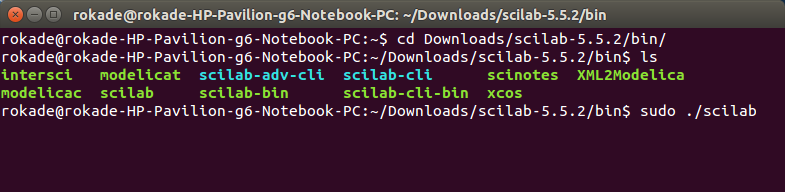
\includegraphics[scale=0.5]{\LocSWfig/linux-cd.png}
      \caption{Linux terminal to launch Scilab}
      \label{linux-cd}
\end{figure}

\subsection{Scilab-Arduino toolbox}
\label{sec:sci-ard-toolbox}
Scilab, by default, does not have the capability to connect to
Arduino. All such add-on functionalities are added to \scilab\ using
toolboxes. Just like we have different installation binaries of
\scilab\ for Windows and Linux, we have different toolboxes types for
Windows and Linux. The \scilab\ Arduino toolbox can be found inside
the {\tt Origin/tools/scilab/windows} or {\tt Origin/tools/scilab/linux} directory,
see \fnrefp{fn:file-loc}.  Use the one depending upon
which operating system you are using. The \scilab\ codes for various
experiments mentioned throughout this book can be found in {\tt
            Origin/user-code} directory. The {\tt user-code} directory will have
many sub-directories as per the experiments.

Let us now see how to load the Scilab-Arduino toolbox. 
\begin{enumerate}
      \item First launch \scilab. On a Windows system, one may start/launch
            \scilab\ either through the Start menu or by double-clicking on the
            shortcut icon created on the Desktop. On a Linux system, one has to
            start \scilab\ through a terminal with root permissions, as
            explained in section \ref{scilab-installation-linux}.
      \item After launching \scilab, first we have to change the working
            directory. Below the menu bar, locate the tab called {\tt File Browser}. 
            Just below {\tt File Browser}, locate a folder-shaped icon. 
            This icon is used to {\tt Select a directory}. Click on this icon.   
            % click on the {\tt File} menu and then click on
            % the {\tt Change current directory} option as shown in
            % \figref{scilab-cd}.
            % \begin{figure}
            %       \centering
            %       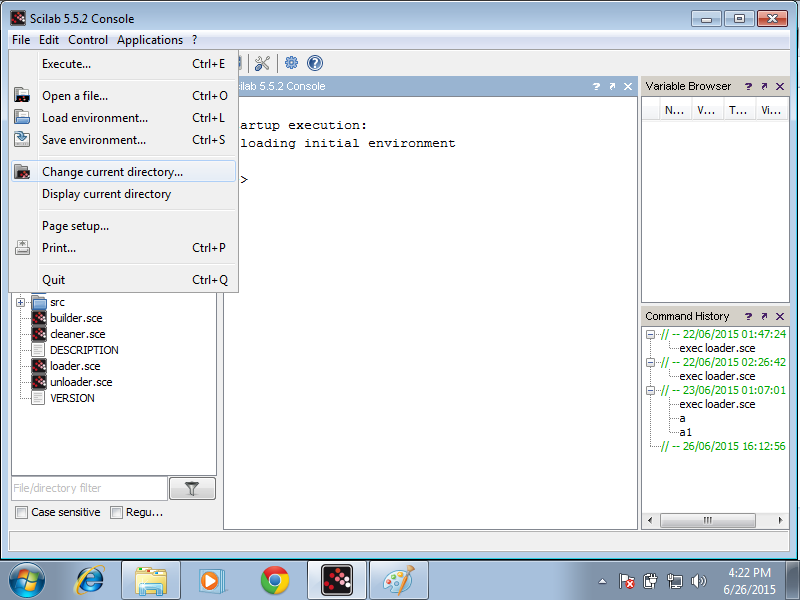
\includegraphics[width=\linewidth]{\LocSWfig/change-directory.png}
            %       \caption{Changing scilab directory}
            %       \label{scilab-cd}
            % \end{figure}
      \item Then, one has to browse to the toolbox folder
                  {\tt Origin/tools/scilab/windows} or {\tt Origin/tools/scilab/linux}, as the case
            may be, and click on, {\tt
                        Open}, as shown in \figref{scilab-browse}.
            \begin{figure}
                  \centering
                  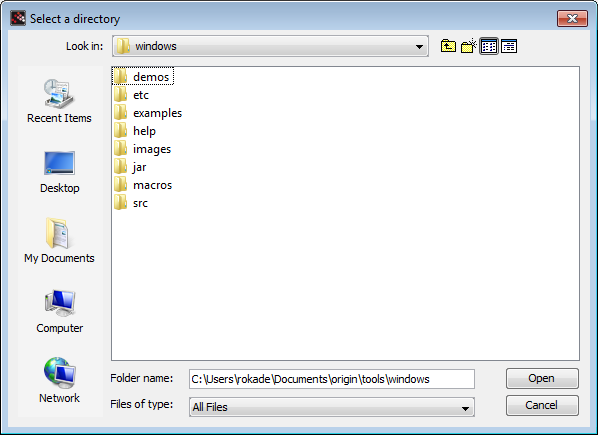
\includegraphics[width=\hgfig]{\LocSWfig/browse-directory.png}
                  \caption{Browsing toolbox directory}
                  \label{scilab-browse}
            \end{figure}
      \item After the previous step, the \scilab\ working directory becomes
            the toolbox folder.  See the {\tt file browser} panel on the
            left-hand side of the \scilab\ console, see \figref{builder}.  It
            will list out the contents of your current working directory. For a
            check, look for the file {\tt builder.sce}.  If you see this file,
            then you are in the right directory.
      \item Next, type the following command on the \scilab\ console: {\tt
            exec builder.sce} - this will build the toolbox and create a file
                  {\tt loader.sce}. This step has to be executed only the first
            time. The output of this step is illustrated in \figref{builder}.
            \begin{figure}
                  \centering
                  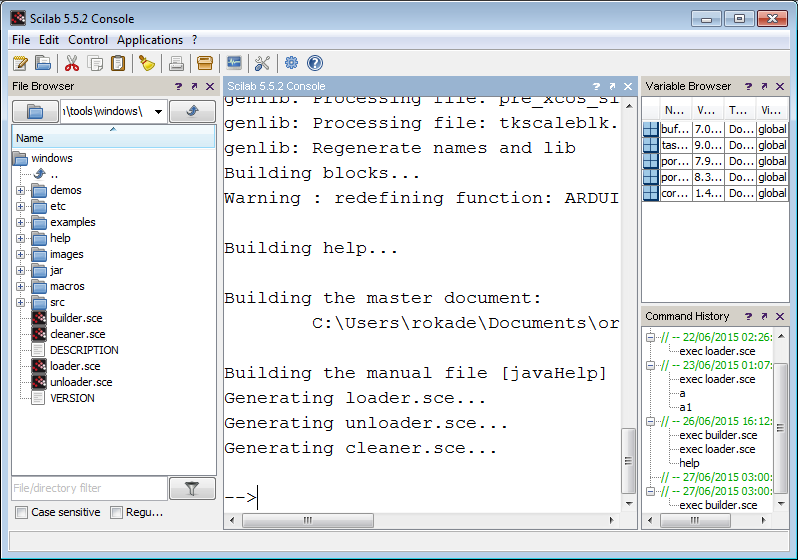
\includegraphics[width=\linewidth]{\LocSWfig/builder.png}
                  \caption{Output of builder.sce}
                  \label{builder}
            \end{figure}
      \item Next, type the command,
            {\tt exec loader.sce} -
            this will load the toolbox. This means all the new functions
            corresponding to the toolbox are loaded in the workspace. It
            will also make available new Xcos blocks, if any.  The
            output of this command is as shown in \figref{loader}.  If you clear
            the workspace for any reason, you will have to execute this command
            once again\footnote{Be careful
                  not to execute the {\tt clear} command.  This will clear the loaded
                  toolbox and you will have to execute the loader.sce file again.}.
            \begin{figure}
                  \centering
                  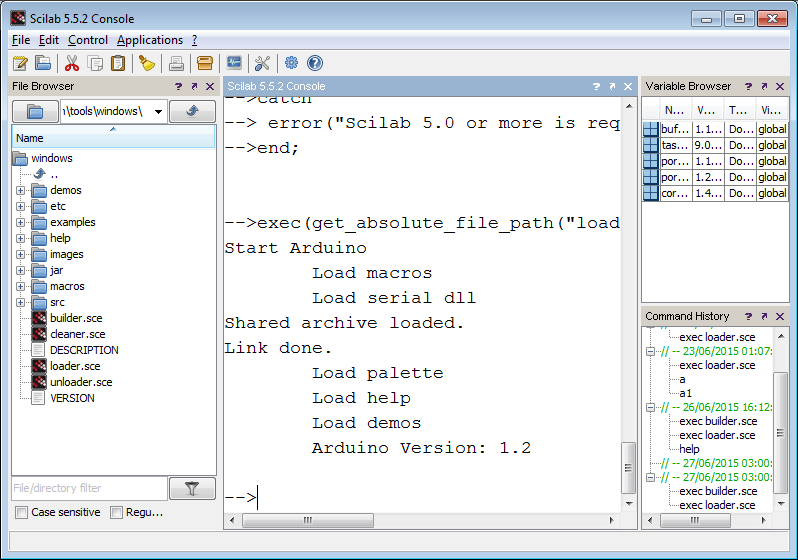
\includegraphics[scale=0.5]{\LocSWfig/loader.png}
                  \caption{Output of loader.sce}
                  \label{loader}
            \end{figure}
\end{enumerate}
The toolbox is now loaded and available for use. 

\subsection{Identifying Arduino communication port number}

Connect \arduino\ board to your computer. On a Windows system, doing
so for the first time will initiate the Windows device identification
routine. It may take a while before it finishes assigning a COM port
number to the \arduino\ board.  If Arduino IDE is installed using the
procedure outlined in \secref{arduino-ide}, required USB drivers for
Arduino get installed automatically.  Hence if you have installed the
Arduino IDE, it should not ask for drivers after you connect it.  As
usually Linux systems come with required drivers, the device is
automatically detected by the OS on connection.

Now let us see how to identify the COM port number. For a Windows
system, open the Device Manager. To do so, right-click on ``My
Computer'' and choose Properties. The Properties window that will open
will have Device Manager in the list on the left-hand side. In the
Device Manager window, look for ``Ports (COM and LPT)''. Double click on
it. It will show you the COM number for \arduino. 

\begin{figure}
      \centering
      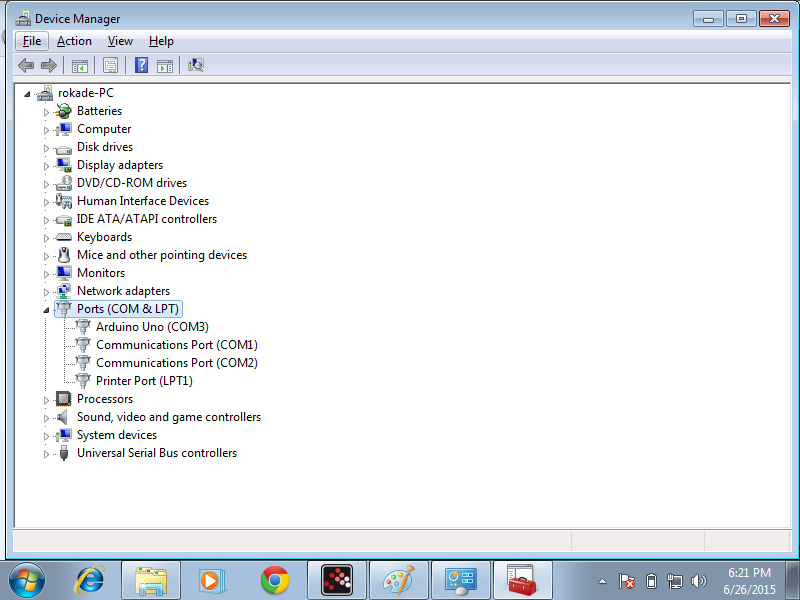
\includegraphics[width=\linewidth]{\LocSWfig/device-manager.png}
      \caption{Device Manager in windows}
      \label{dev-mgr}
\end{figure}

The result of the above exercise is shown in \figref{dev-mgr}.  In
this case, the system has detected Arduino with port number 3, which
appears as COM3.  In this book, we have taken the port for
communication as 2 and written code consistent with this assumption.    
As a result, we will now change it to
COM2\footnote{\label{fn:port}It is possible to leave it at whatever
      port number one gets.  It is also possible to choose any number
      between 2 and 99.  In this case, the port number should be
      changed accordingly in the code.  We will point this out throughout
      the book.}.  To change the port number, double click on the port
number. Its properties window will appear. Click on the ``Port
Settings'' tab and then click on ``Advanced'' button as shown in
\figref{com}.

\begin{figure}
      \centering
      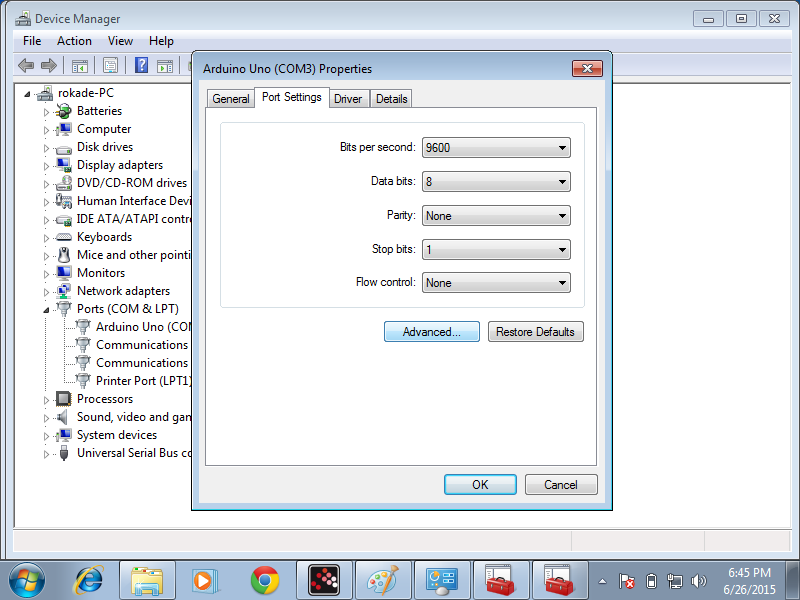
\includegraphics[scale=0.5]{\LocSWfig/com-properties.png}
      \caption{COM port properties window}
      \label{com}
\end{figure}

Click on the drop-down menu for COM port numbers. Choose the port
number COM2.  On clicking on ``OK'', Windows may warn you that the port
number is already in use. But given that you do not have any other USB
device connected you may force change it. Click on ``OK'' to close
all of the device manager windows. Now, we are set to go ahead with
port number 2. The stress on using port number 2 is just to be
consistent throughout the book. It is mainly for a beginner.

Now, let us see how to identify the port number on a Linux
system. Open a terminal by pressing Alt+Ctrl+T keys together. Then
type the following command and press enter, {\tt ls
            /dev/ttyACM*} -
the output of this command is shown in \figref{linux-port}. It has
detected the Arduino with the port number ``ttyACM0''.  The last character
in this string, namely 0, is the port number.  You may get 0 or a
number such as 1 or 2 in your case, for the port number.

\begin{figure}
      \centering
      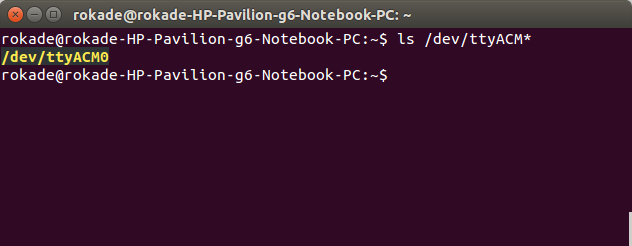
\includegraphics[scale=0.5]{\LocSWfig/linux-port.png}
      \caption{Port number on Linux terminal}
      \label{linux-port}
\end{figure}

\subsection{Testing Scilab-Arduino toolbox}
\label{sec:testing-scilab-arduino}
Now let us test the functioning of the toolbox. 
\begin{enumerate}
      \item Install Arduino IDE, as explained in \secref{sec:ard-start} and
            launch it.
      \item Read into the Arduino IDE, the firmware \ardref{ard:firmware}.
      \item Using the {\tt Upload} option of the Arduino IDE, load this
            firmware on to the \arduino\ board.
      \item Inside the {\tt Origin/tools/scilab} directory, locate a file {\tt
                        test\_firmware.sce}. This file will be used to test whether the
            firmware is properly installed.  This is an important step, as the
            connection between the computer and Arduino breaks down sometimes.
            The Scilab toolbox is unable to identify this difficulty - it has to
            be externally done.  If this difficulty is not identified and
            rectified, one will waste a lot of time and effort trying to debug
            the error.  This test has to be done in case of difficulties.
      \item In the \scilab\ console, type {\tt editor} and press the enter
            key. This will launch the editor. Click on ``File'' menu and choose
            ``Open''. Browse to the directory {\tt Origin/tools/scilab} and choose the
            file {\tt test\_firmware.sce}.  It will open
            \sciref{sci:test-firmware}.  
            %The \scilab\ editor with this file open is as shown in \figref{test-code}.
            %   \begin{figure}
            %     \centering
            %     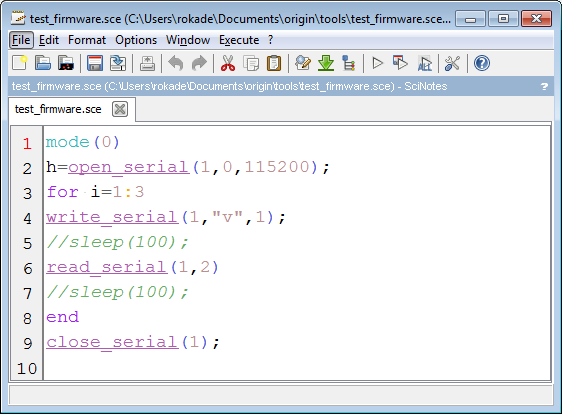
\includegraphics[scale=0.5]{\LocSWfig/test-code.png}
            %     \caption{Scilab code to test toolbox and firmware}
            %     \label{test-code}
            %   \end{figure}
            
      \item If you are using a Windows system and have set your port number
            as COM2, you need not make any changes to the file. Linux users,
            however, will mostly identify the port number as ``ttyACM0''. Hence, 
            they need to change the following line number
            \lstinputlisting[firstline=2,lastline=2]
            {\LocSWchkcode/test_firmware.sce}
            to
            \begin{lstlisting}[style=nonumbers]
  h = open_serial(1,0,115200); 
\end{lstlisting}
            
      \item To execute this code, on the menu bar, click on the {\tt
                        Execute}, option. Then choose {\tt File with no echo}. The output
            will appear on the Console as shown in \figref{test-console}.
            \begin{figure}
                  \centering
                  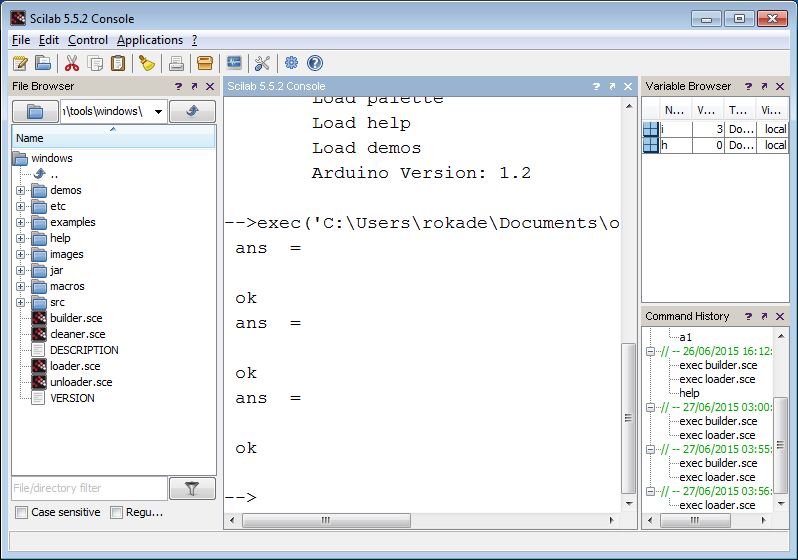
\includegraphics[scale=0.5]{\LocSWfig/test-console.png}
                  \caption{Scilab test code output}
                  \label{test-console}
            \end{figure}
            As shown in the figure, we see the response of this code as ``ans = '' and
            ``ok'' three times.  The
            code basically gives some input to Arduino three times and the
            program inside it returns ``ok'' three times.  This code thus confirms
            the working of the Scilab-Arduino toolbox.  The code also confirms
            that the firmware inside the Arduino is correct.  It is alright if
            one or two of the attempts out of three give a blank response.  But
            all the three responses certainly should not be
            blank\footnote{\label{fn:firmware}If this step is unsuccessful,
                  one should check the connections and re-install the firmware}.
\end{enumerate}

Now let us take a look at the various functions facilitated by the
toolbox. The functions provided in the toolbox are as shown in 
\figref{func}. They are basically categorized into four categories:
configuration, digital, analog and motors. These functions will be
explained in detail in the subsequent chapters as and when they are
used.

\begin{figure}
      \centering
      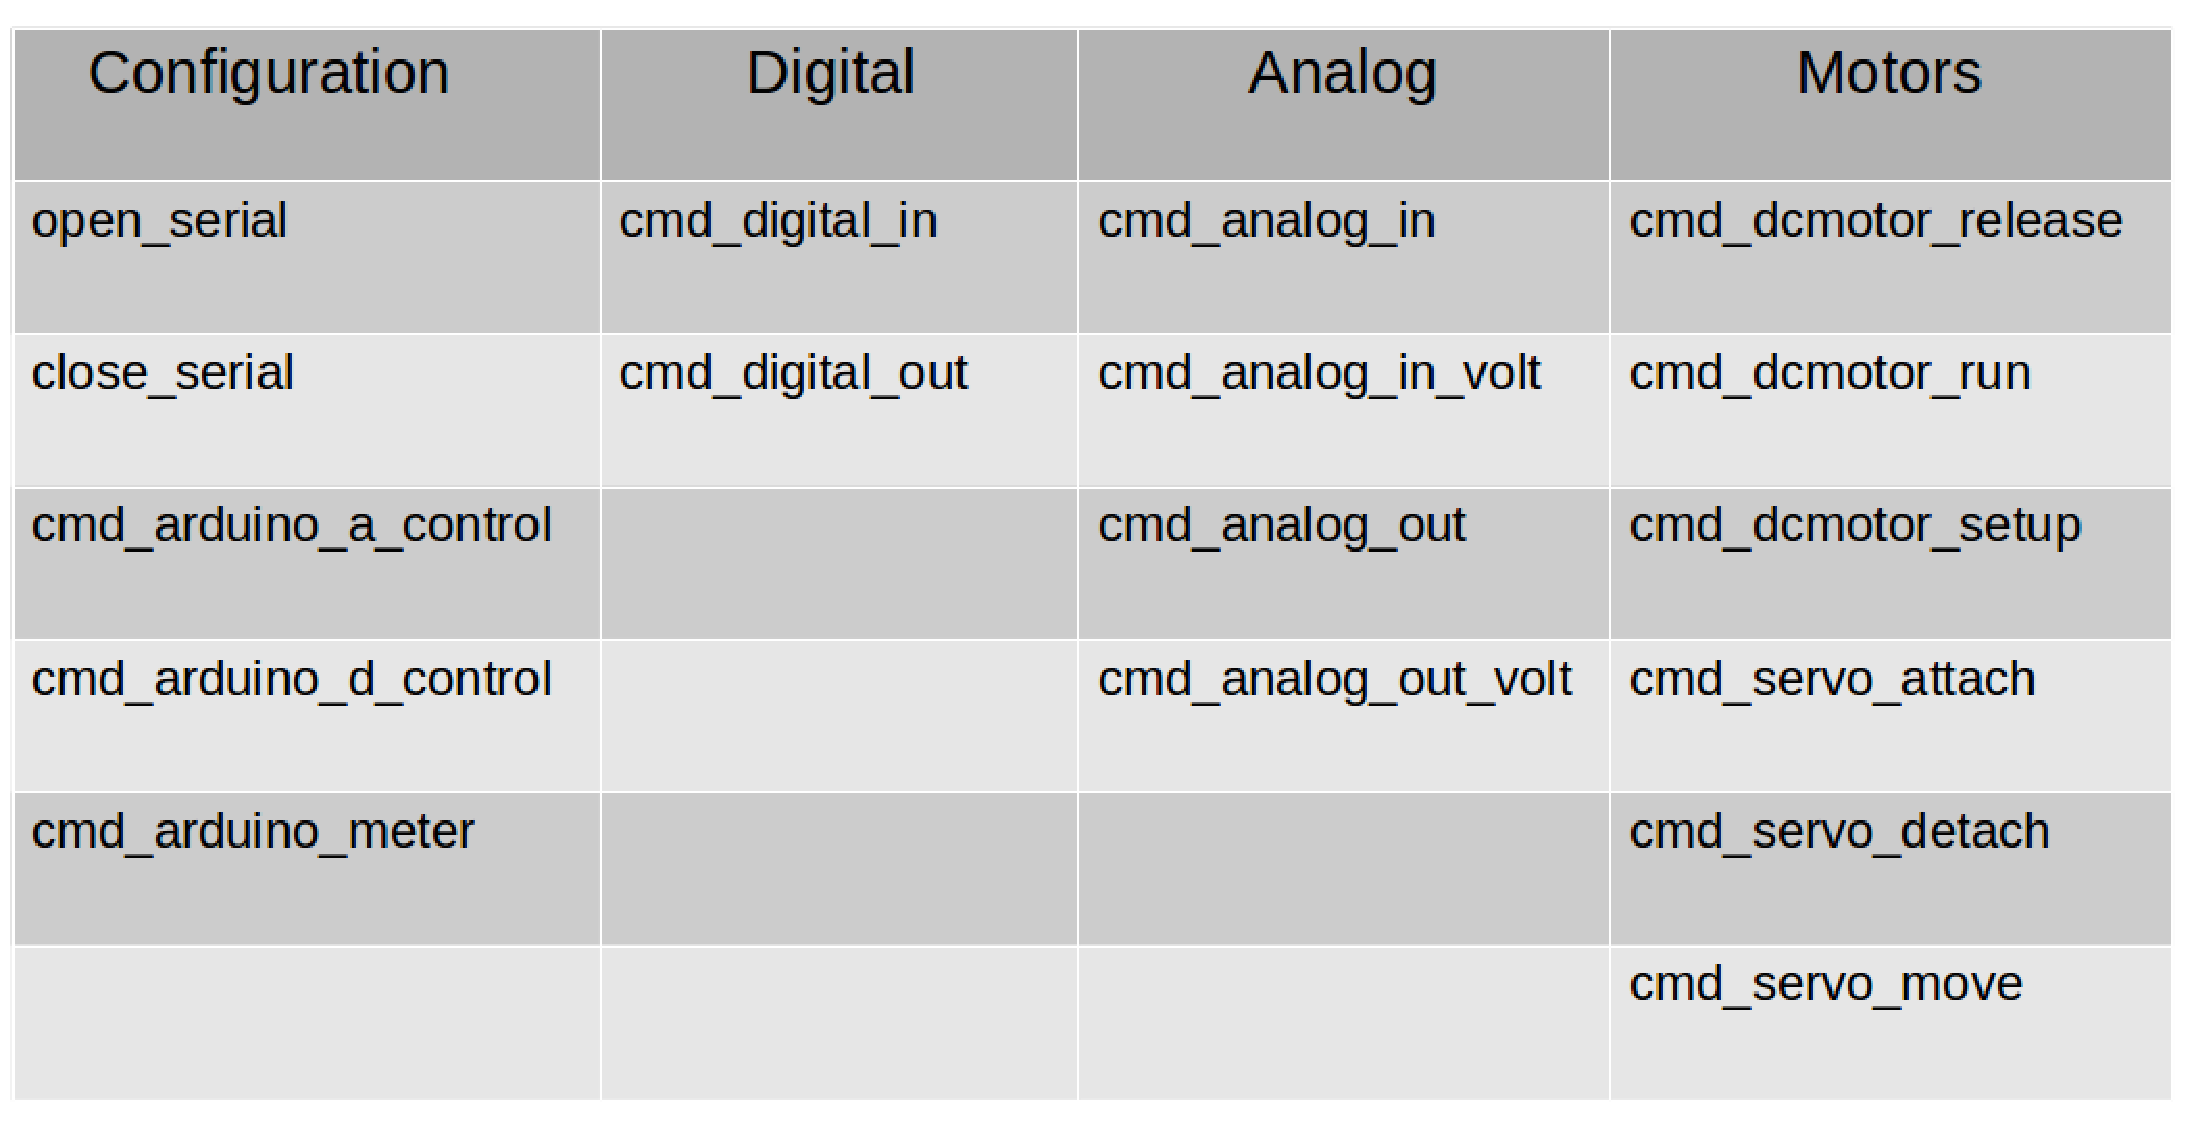
\includegraphics[width=\linewidth]{\LocSWfig/table_functions_crop.pdf}
      \caption{Arduino toolbox functions used in this book}
      \label{func}
\end{figure}

\subsection{Firmware}
\lstset{style=mystyle}
\label{sec:test-firmware-scilab}
\addtocontents{cod}{\protect\addvspace{\codclr}}
We have provided a Scilab code to check whether the firmware has been
properly installed.  That code is listed below.

\begin{scicode}
      \ccaption{A Scilab code to check whether the firmware is
            properly installed or not}{A Scilab code to check whether the
            firmware is properly installed or not.  Available at 
            \LocSWchkbrief{test\_firmware.sce}. Execute this code 
            by following the steps given in section 
            \ref{sec:testing-scilab-arduino}.}
      \label{sci:test-firmware}
      \lstinputlisting{\LocSWchkcode/test_firmware.sce}
\end{scicode}


\section{Xcos}
\label{sec:xcos-start}
Xcos is a graphical editor for \scilab\ \cite{xcos-ref}. Most of the
mathematical manipulations that can be done using \scilab\ scripts,
can be done using Xcos also.  The major advantage of Xcos is the
intuitive interface and easy connectivity across blocks. Xcos even
supports {\tt if else}, {\tt for}, and {\tt while} looping which forms
an integral part of any programming language. It is possible to code
the entire algorithm using Xcos blocks alone. It is also possible to
read from and write to the \scilab\ workspace through Xcos.

\subsection{Downloading, installing and testing}
Xcos comes pre-installed with \scilab. Hence a separate installation
of Xcos is not required. Let us explore the functionalities Xcos has
to offer. Xcos basically provides a graphical interface to \scilab.  

Xcos can be launched from \scilab\ by clicking on the Xcos icon
available on the \scilab\ menu bar. It can also be launched by simply
typing the command {\tt xcos} in the \scilab\ console. When Xcos is
launched, it will open a palette browser.  We have shown this in
\figref{sine-blk}, where we have selected a sine block.  At the time
of launch, Xcos will also open an empty canvas, called an untitled
Xcos window.

\begin{figure}
      \centering
      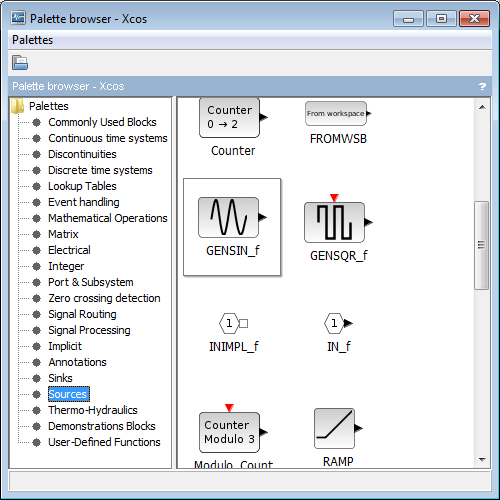
\includegraphics[width=\hgfig]{\LocSWfig/sine-blk.png}
      \caption{Sine generator in palette browser}
      \label{sine-blk}
\end{figure}

% \begin{figure}
% \centering
% 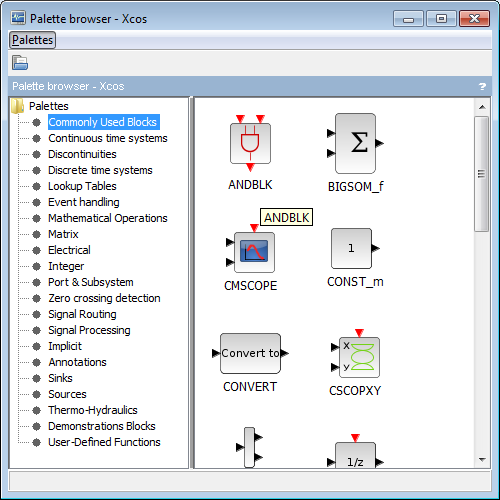
\includegraphics[scale=0.5]{\LocSWfig/palette-browser.png}
% \caption{Palette Browser}
% \label{palette}
% \end{figure}


% \begin{figure}
% \centering
% 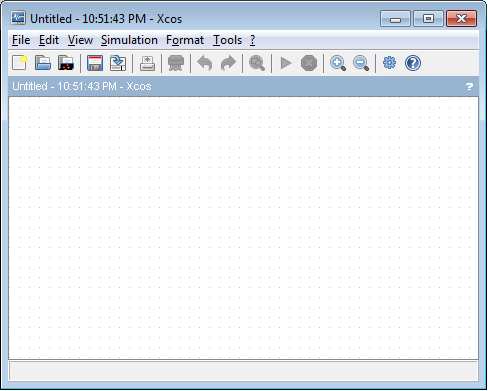
\includegraphics[scale=0.5]{\LocSWfig/untitled-xcos.png}
% \caption{Untitled Xcos window}
% \label{untitled}
% \end{figure}

Palette browser shows all of the available blocks that can be used. It
has been nicely categorized as per the functionality. For example,
blocks that generate signals/values without any input, fall under the
category {\tt Sources}. Similarly, blocks that take signals/values
without giving any output are categorized as {\tt Sinks}. This makes
finding a particular block very easy, specially when one does not know
the name of a block.

The untitled window is the one where one creates the Xcos
code/diagram. The relevant blocks have to be dragged and dropped from
the palette browser to the untitled window. The blocks are then
interconnected and configured as per the simulation, which we will
demonstrate next.

\subsection{Use case}
Let us build a simple Xcos simulation to plot a sine wave. This
simulation requires a sine wave source. It can be found in the {\tt
            Sources} category as shown in \figref{sine-blk}. Drag and drop this
block in the untitled Xcos window. 

Next, we need a block to plot the sine wave. A plotting block can be
found in the {\tt Sinks} category as shown in \figref{plot-blk}. The
name of this block is CSCOPE. Drag and drop this block in the untitled
Xcos window.  On the left-hand side, this block has an input port for
data.  It is black in colour, which may not be obvious in a black and
white printout.  The output from the sine block has to be connected
to this port.  At its top side, the CSCOPE block has another input
port, called an event port.  This is red in colour.  This port is used
to synchronize it with event generating devices.

\begin{figure}
      \centering
      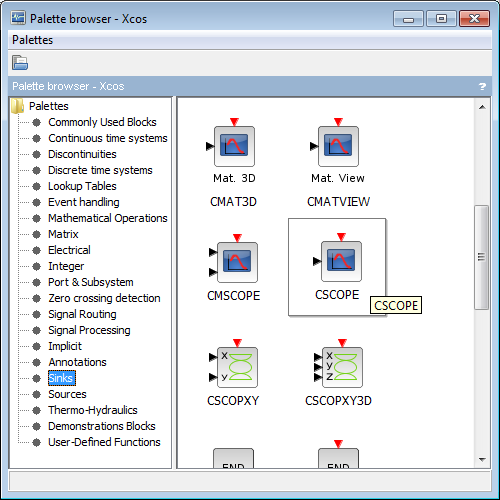
\includegraphics[width=\hgfig]{\LocSWfig/plot-blk.png}
      \caption{CSCOPE block in xcos}
      \label{plot-blk}
\end{figure}

As the CSCOPE block has an
input event port, we need a source that generates events. Hence, the
next block that we need is an event generator block and it can be
found in the {\tt Sources} category. This is illustrated in figure
\ref{clk-blk}. The name of this block is CLOCK\_c. Drag and drop this
block in the untitled Xcos window.

\begin{figure}
      \centering
      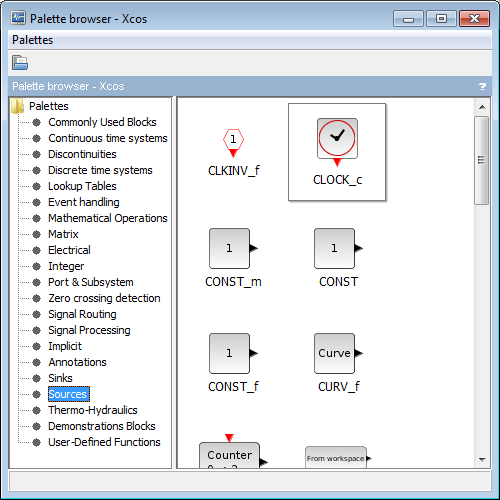
\includegraphics[width=\hgfig]{\LocSWfig/clock-blk.png}
      \caption{CLOCK\_c block in xcos}
      \label{clk-blk}
\end{figure}

The next step is to interconnect the blocks together. A black color
port can only be connected to another black color port. A black color
port cannot be connected to a red color port and vice versa.  That is,
a data port cannot be connected to an event port.  Linking
two blocks is a bit crucial and may need a few attempts before one gets
comfortable. To link two blocks, first click and hold the left mouse
button over the output port of the source block. Without releasing the
mouse button, touch the mouse pointer to the input port of the sink
block. If a connection is possible there, the port will turn
``green''. At this point, release the mouse button and the blocks should
get connected. Follow this procedure and complete the connection as
shown in \figref{sine-gen}.  Save this file with the name {\tt
            sine-generator}.  

\begin{figure}
      \centering
      \includegraphics[width=\smfig]{\LocSWfig/sine-gen.png}
      \caption{Sine generator in Xcos}
      \label{sine-gen}
\end{figure}

Let us simulate this Xcos code. On the menu bar, click on the {\tt
            Simulation} menu and choose {\tt Start}. You will get a graphic
window with a running sine wave as shown in \figref{sine-output}.

\begin{figure}
      \centering
      \includegraphics[width=\lgfig]{\LocSWfig/sine-output.png}
      \caption{Sine generator Xcos output}
      \label{sine-output}
\end{figure}

This is because we are running the simulation using the default
configuration.  We would like a stationary plot.  If the simulation is
still running, go to the Simulation menu and choose Stop.  Double
click on the CSCOPE block. Its properties window will appear as shown
in \ref{cscope-config}. Note the value of the {\tt Refresh period}. It
is by default 30. Click on Ok.

\begin{figure}
      \centering
      \includegraphics[width=\lgfig]{\LocSWfig/cscope-config.png}
      \caption{CSCOPE configuration window}
      \label{cscope-config}
\end{figure}

Next, on the menu bar, click on the {\tt Simulation} menu and choose
      {\tt Setup}. The {\tt Set Parameters} window will open. The first
parameter is {\tt Final integration time}. It decides for how long the
simulation will run. Change it to be equal to the {\tt Refresh period}
of the CSCOPE block.  That is, change it to 30 as shown in
\figref{sim-setup}. Now start the simulation and you will get a static
plot.  Other paramenters of blocks can also be changed. For example,
one may want to change the input amplitude/frequency or change the
plot scales, etc. All these are left to the reader to explore.

\begin{figure}
      \centering
      \includegraphics[width=\lgfig]{\LocSWfig/sim-setup.png}
      \caption{Simulation setup window}
      \label{sim-setup}
\end{figure}

Although we have demonstrated a very basic level of Xcos simulation,
this idea can be used for complex processes as well.  Using Xcos, it
is possible to have user-defined blocks. The user can code the
working of the block as a function in \scilab\ script and then call it
from Xcos.  It is also possible to create subsystems.  
One can even read from and write to C binaries.  Xcos comes with
several pre-defined libraries and hence, it is possible to carry out
other kinds of simulation, such as electrical circuit simulation and
basic thermo-hydraulic simulation, for example.  A detailed 
explanation and demonstration are beyond the scope of this book.


\subsection{Xcos-Arduino}
The \scilab\ Arduino toolbox not only provides functions to be used in
\scilab\ scripts but also provides new Arduino-specific blocks. As
shown in \figref{arduino-palette} new Arduino blocks are now available
for use.  Similar to the categorization of the functions, the Xcos
blocks are also categorized as configuration, digital, analog and
motors. Again, it is possible to conduct the experiments only using
Xcos. Xcos codes for every experiment are provided throughout the
book. The Arduino blocks can be easily connected to Xcos native
blocks. A detailed block help for every block can be sought by right-clicking on the block and choosing ``Block help''. This is illustrated
in \figref{blk-help}.

\begin{figure}
      \centering
      \includegraphics[width=\lgfig]{\LocSWfig/arduino-palette.png}
      \caption{Palette browser showing Arduino blocks}
      \label{arduino-palette}
\end{figure}

\begin{figure}
      \centering
      \includegraphics[width=\lgfig]{\LocSWfig/xcos-help.png}
      \caption{Xcos block help}
      \label{blk-help}
\end{figure}

%%%%%python description starts
\section{Python}
\label{sec:python-start}
Python is a general-purpose, high-level, remarkably powerful dynamic programming language 
that is used in a wide variety of application domains. Its high-level built-in data structures, 
combined with dynamic typing and dynamic binding, make it very attractive for Rapid Application Development, 
as well as for use as a scripting or glue language to connect existing components together. 
Python's simple, easy to learn syntax emphasizes readability and therefore reduces the cost of program maintenance. 
Python supports modules and packages, which encourages program modularity and code reuse. 
The Python interpreter and the extensive standard library are available in source or binary form without 
charge for all major platforms, and can be freely distributed \cite{python-ref}.


\subsection{Downloading and installing on Windows} \label{py-windows}
This book uses Python 3 for demonstrating the experiments, both on Windows 
and Linux. Since Python uses indentation to indicate a block of code, 
the users are advised to install a programmer text editor like Atom. 
This editor will allow the readers to modify the Python scripts on their 
machines if they want to. Starting from download, we shall go through the 
steps to set up Python 3 on Windows OS:

\begin{enumerate}
      \item Visit the URL {\tt https://www.python.org/}. 
      At the top of the page, locate the Downloads tab and click on it. 
      At the time of writing this book (as of 21 April 2021), Python 3.9.4 
      is the latest version. Click on Download Python 3.9.4 to download the 
      executable file. The readers may want to download the other versions of 
      Python 3. However, we recommend the installation of Python 3.5 or above. 
      It may be noted that some of the Python 3 versions cannot be used on Windows 7 or earlier.
      \item Locate the executable file and double-click on it to begin the 
      installation. Python 3.9.4 Setup window appears, as shown in \figref{python-windows}. 
      In this window, check the box which says, Add Python 3.9 to PATH and 
      click on Install now.  
      \begin{figure}
            \centering
            \includegraphics[width=\lgfig]{\LocSWfig/python-windows-install.JPG}
            \caption{Installing Python 3 on Windows}
            \label{python-windows}
      \end{figure}
\end{enumerate}

Once the installation is finished, Python 3.9 App can be launched 
from the Start menu. In this book, we will use the Command Prompt to 
execute the Python scripts. Please note that a Python script has .py as its 
extension. Carry out the steps given below to execute a Python script from 
the Command Prompt:

\begin{enumerate}
      \item Launch the Command Prompt. Press the Windows key+R together. 
      A window, as shown in \figref{windows-run} appears. In the text box adjacent to {\tt Open}, type {\tt cmd}, 
      and press Enter. The Command Prompt, as shown in \figref{windows-cmd} appears. 
      By default, it points to the home directory.  
      \begin{figure}
            \centering
            \includegraphics[width=\lgfig]{\LocSWfig/windows-cmd.png}
            \caption{Launching the Command Prompt on Windows}
            \label{windows-run}
      \end{figure}
      \item Now, we will check whether Python 3.9 was installed 
      successfully or not. In the Command Prompt, type {\tt py -{}-version} and 
      press Enter. If this step displays Python 3.9.4 in the following line, 
      the installation was successful. 
      \begin{figure}
            \centering
            \includegraphics[width=\lgfig]{\LocSWfig/win-command-prompt.png}
            \caption{Command Prompt on Windows}
            \label{windows-cmd}
      \end{figure}
      \item Using the {\tt cd} command, navigate to the directory where your Python 
      script is located. Assuming that your Command Prompt points to the 
      home directory, and you want to navigate to the folder Origin on 
      Desktop, execute the following command: {\tt cd Desktop\textbackslash Origin} \\
      It may be noted that a backslash (\textbackslash) has been used between 
      Desktop and Origin. 
      \item To view the contents of this folder, type {\tt dir} and press Enter.
      \item Suppose you have a Python script named  {\tt FILENAME.py} in this 
      folder. To execute this script, type {\tt python FILENAME.py} and press 
      Enter. The required output will be displayed in the Command Prompt itself. 
      We don’t expect the readers to run the command {\tt python FILENAME.py} at 
      this instant. This command will be helpful while running the Python 
      scripts in the upcoming sections and chapters. 
      \item To exit the Command Prompt, type {\tt exit} and press Enter. 
 
\end{enumerate}

Apart from Python, we need to install Python Serial Port Extension, 
also known as pyserial \cite{pySerial}. To do so, carry out the steps given 
below:
\begin{enumerate}
      \item Launch the Command Prompt, as shown in \figref{windows-run}. 
      \item First, we need to make sure we have pip available. 
      In the Command Prompt, execute the following command: {\tt py -m pip -{}-version} \\ 
      This step should display an output with the version of pip installed. 
      \item Now, install pyserial. In the Command Prompt, execute the following command: 
      {\tt py -m pip install pyserial}  
      \item We will verify whether the pyserial package was installed successfully or not. 
      In the Command Prompt, execute the following command: 
      {\tt pip show pyserial}
      It should show the name, version, etc., of the package. 
      \item To exit the Command Prompt, type {\tt exit} and press Enter. 
\end{enumerate}

\subsection{Downloading and installing on GNU/Linux Ubuntu} \label{py-linux}
On Linux, we can install Python from the terminal. Please ensure that you 
are connected to the Internet. To install Python 3.5, carry out the steps given below:
\begin{enumerate}
      \item Open a terminal by pressing the Alt+Ctrl+T keys together.
      \item Update the system by executing the command {\tt sudo apt-get update}
      \item Install Python3.5 by executing the command given below:\\
      {\tt sudo apt-get install python3.5}
      \item Now, we will check whether Python was installed 
      successfully or not. In the terminal, type {\tt py -{}-version} and 
      press Enter. If this step displays Python 3.8.4 in the following line, 
      the installation was successful. 
\end{enumerate}

Once the installation is finished, Python 3 can be launched 
from the terminal. In this book, we will use the Linux terminal to 
execute the Python scripts. Please note that a Python script has .py as its 
extension. Carry out the steps given below to execute a Python script from 
the terminal:
\begin{enumerate}
      \item Open a terminal by pressing the Alt+Ctrl+T keys together.
      \item Using {\tt cd} command, navigate to the directory where the Python script is located. 
      \item Suppose you have a Python script named  {\tt FILENAME.py}. 
      To execute this script, type {\tt python3 FILENAME.py} and press 
      Enter. The required output will be displayed in the terminal itself. 
      We don’t expect the readers to run the command {\tt python3 FILENAME.py} at 
      this instant. This command will be helpful while running the Python 
      scripts in the upcoming sections and chapters. 
\end{enumerate}

Apart from Python, we need to install Python Serial Port Extension, 
also known as pyserial \cite{pySerial}. To do so, carry out the steps given 
below:
\begin{enumerate}
      \item Open a terminal by pressing the Alt+Ctrl+T keys together.
      \item First, we need to install pip. In the terminal, execute the following command: 
      {\tt sudo apt-get install python3-pip} 
      \item Now, install pyserial. In the terminal, execute the following command:\\ 
      {\tt pip3 install pyserial}  
      \item We will verify whether the pyserial package was installed successfully or not. 
      In the terminal, execute the following command: 
      {\tt pip3 show pyserial}\\
      It should show the name, version, etc., of the package. 
\end{enumerate}

% \begin{enumerate}
%       \item On Ubuntu, Python can be installed from the command line by typing in the
%             following commands:

%             \$ sudo apt-get install python3.5 \\
%             This will install python 3.5 as this set of tools are compatible with python3. It also
%             works all other versions of python3.  
%             \$ pip3 install python-serial \\
%             This will install serial package required for communicating with Arduino Uno.
%       \item 1. On Windows,


%             Download Windows python compiler Self Extracting Archive (.exe)  (32-bit or 64-bit as per your system) from https://www.python.org/downloads/windows/

%             Download Windows pyserial package .exe from https://pypi.python.org/pypi/pyserial/3.4.
%             After downloading run the .exe file and follow the instructions.

%             Now that we have Python installed, open the terminal by typing 'Ctrl+Alt+T'.
%             Enter the command 'python'. This opens the Python REPL (Read Eval Print Loop).
%             Python files have .py extension and .py files can be executed by typing "python3 filename.py"
%             on the python terminal. Please visit the link https://github.com/manasdas17/Python3-Arduino for 
%             the library. 

% \end{enumerate}

\subsection{Python-Arduino toolbox}
\label{sec:python-toolbox}
Python, by default, does not have the capability to connect to Arduino. 
All such add-on functionalities are added to Python using packages. 
The Python-Arduino toolbox can be found inside the {\tt Origin/tools/python} directory, 
see \fnrefp{fn:file-loc}.  This toolbox is compatible for both of the operating systems: Windows and Linux. 
The Python scripts (or codes) for various experiments mentioned throughout this book can be found in 
{\tt Origin/user-code} directory. The {\tt user-code} directory will have many sub-directories as per the experiments. 

In this book, we have created a package named "Arduino" in Python 3.  This package is available at 
{\tt Origin/tools/python}. This package makes use of the functions available in pyserial \cite{pySerial} to 
establish serial communication with Arduino. In this package, we have added functions required to run 
various experiments on \arduino. Using this basic set of functions, the user can define other functions to operate
upon the Arduino. Please note that the "Arduino" package and the FLOSS firmware  given 
in \ardref{ard:firmware} are required to run the experiments. 

Now, we will see how to import (or load) the "Arduino" package inside a Python script to run 
various experiments provided in this book. In a Python script, add {\tt from Arduino.Arduino import Arduino} 
at the top of the script. When we add {\tt from Arduino.Arduino import Arduino} in a script, the function "from" 
searches for "Arduino" only in that directory where our script is saved. That's why all the scripts in Python 
must be saved in a folder that contains the "Arduino" package. In this book, "Arduino" package has been saved 
in the folder where the Python scripts for each chapter are available. For the sake of convenience, we have 
added {\tt from Arduino.Arduino import Arduino} in all the Python scripts provided in this book. 
To run a particular experiment, one can follow the steps as given in \secref{py-windows} or \secref{py-linux}. 


\subsection{Firmware}
\lstset{style=mystyle}
\label{sec:test-firmware-python}
\addtocontents{pyd}{\protect\addvspace{\codclr}}
We have provided a Python code to check whether the firmware has been properly installed. That code is listed below.  
Please ensure that you have uploaded the FLOSS firmware given in \ardref{ard:firmware} on the \arduino\ board.

\begin{pycode}
      \pcaption{A Python script to check whether the firmware is properly installed
            or not}{A Python script to check whether the firmware is properly installed
            or not.  Available at 
            \LocFIMpybrief{test\_firmware.py}. 
            Execute this script by following the steps given in \secref{py-windows} or \secref{py-linux}. If the execution is
            successful, you should expect three "ok" messages.}
      \label{py:test-firmware}
      \lstinputlisting{\LocFIMpycode/test_firmware.py}
\end{pycode}



%%%%%python description ends

%%%%%%Julia descrition starts

\section{Julia} \label{sec:julia-start}
Julia is a high-level, high-performance dynamic programming language for 
technical computing, with a syntax familiar to users of other technical computing 
environments \cite{julia-ref}. While it is a general-purpose language and can be used to write any 
application, many of its features are well suited for numerical analysis and 
computational science. Julia provides a sophisticated compiler, distributed 
parallel execution, numerical accuracy, and an extensive mathematical function
library. 

% This is a set of tools that provide functionality in Julia, to program the \arduino. 

\subsection{Downloading and installing on Windows} \label{julia-install-windows}
This book uses Julia 1.6.0 for demonstrating the experiments, both on Windows and Linux. 
Julia does not use indentation to indicate a block of code, unlike Python. However, 
the users are advised to install a programmer text editor like Atom. This editor will 
allow the readers to modify the Julia source files on their machines if they want to. 
Alternatively, one can also use Notepad (on Windows) or gedit (on Linux Ubuntu) to edit 
Julia source files. Starting from download, we shall go through the steps to set 
up Julia 1.6.0 on Windows OS:
\begin{enumerate}
      \item Visit the URL {\tt https://julialang.org/}.  At the top of the page, 
      locate the Download tab and click on it. From the Current stable release, 
      download the required Julia binaries (32 or 64-bit) for Windows, as shown in \figref{julia-download}. 
      At the time of writing this book, the Current stable release refers to Julia 1.6.0 
      as of March 24, 2021, as shown in \figref{julia-download}. In this book, we will perform 
      experiments with a 64-bit installation of Julia 1.6.0.
      \item Locate the executable file. Right-click on it and hit 
      Run as administrator to begin the installation. After selecting the Installation Directory, 
      a window named Select Additional Tasks appears as shown in \figref{julia-windows-install}. 
      In this window, check the box which says, Add Julia to PATH and click on Next to continue the installation. 
\end{enumerate}

\begin{figure}
      \centering
      \includegraphics[width=\textwidth]{\LocSWfig/julia-download.png}
      \caption{Julia's website to download 64-bit Windows/Linux binaries}
      \label{julia-download}
\end{figure}

\begin{figure}
      \centering
      \includegraphics[width=\lgfig]{\LocSWfig/julia-windows-install.png}
      \caption{Installing Julia 1.6.0 on Windows}
      \label{julia-windows-install}
\end{figure}

Once the installation is finished, Julia 1.6.0 App can be launched either 
from the Start menu or from the Command Prompt. In this book, we will use the Command 
Prompt to execute the Julia source files. Please note that a Julia source file has .jl as its extension. 
Carry out the steps given below to execute a Julia source file from the Command Prompt:
\begin{enumerate}
      \item Launch the Command Prompt. Press the Windows key+R together. A window, as shown in \figref{windows-run} 
      appears. In the text box adjacent to Open, type cmd, and press Enter. The Command Prompt, as shown in
       \figref{windows-cmd} appears. By default, it points to the home directory.
      \item Now, we will check whether Julia 1.6.0 was installed successfully or not. 
      In the Command Prompt, type {\tt julia -{}-version} and press Enter. 
      If this step displays julia version 1.6.0 in the following line, the installation was successful.
      \item Using the {\tt cd} command, navigate to the directory where your Julia source file is located. 
      Assuming that your Command Prompt points to the 
      home directory, and you want to navigate to the folder Origin on 
      Desktop, execute the following command: {\tt cd Desktop\textbackslash Origin} \\
      It may be noted that a backslash (\textbackslash) has been used between 
      Desktop and Origin. 
      \item To view the contents of this folder, type {\tt dir} and press Enter.
      \item Suppose you have a Julia source file named {\tt FILENAME.jl} in this 
      folder. To execute this script, type {\tt julia FILENAME.jl} and press 
      Enter. The required output will be displayed in the Command Prompt itself. 
      We don't expect the readers to run the command {\tt julia FILENAME.jl} at 
      this instant. This command will be helpful while running the Python 
      scripts in the upcoming sections and chapters. 
      \item To exit the Command Prompt, type {\tt exit} and press Enter. 
\end{enumerate}

Apart from Julia, we need to install the SerialPorts \cite{julia-serial-ports} package in Julia. This package will be
required to establish serial communication with Arduino boards. Please make sure that 
you are connected to the Internet. To install the package, we will use {\tt Pkg}. 
It is Julia's built-in package manager and handles operations such as installing, 
updating and removing packages in Julia. To install the SerialPorts package, carry out the steps given below:
\begin{enumerate}
      \item Launch the Command Prompt, as shown in \figref{windows-run}.
      \item In the Command Prompt, type {\tt julia} and press Enter. It should launch Julia in an interactive session (also known as a read-eval-print loop or "REPL"), as shown 
      in \figref{julia-repl-windows}. When run in interactive mode, Julia displays a banner and 
      prompts the user for input. By default, Julia REPL appears in Julian prompt. It is the default mode of 
      operation; each new line initially starts with {\tt julia>}, as 
      shown in \figref{julia-repl-windows}. It is here that you can enter Julia expressions. 
      Hitting return or Enter after a complete expression has been entered will evaluate 
      the entry and show the result of the last expression. 
      \begin{figure}
            \centering
            \includegraphics[width=\textwidth]{\LocSWfig/julia-repl-windows.png}
            \caption{Windows command prompt to launch Julia REPL}
            \label{julia-repl-windows}
      \end{figure}
      \item Now, we need to enter the {\tt Pkg} REPL in Julia. From the Julia REPL, 
      press {\tt ]} to enter the {\tt Pkg} REPL. The moment you press 
      {\tt ]}, you enter {\tt Pkg} REPL, as shown in \figref{julia-pkg-windows}.
      \begin{figure}
            \centering
            \includegraphics[width=\textwidth]{\LocSWfig/julia-pkg-windows.png}
            \caption{Windows command prompt to enter Pkg REPL in Julia}
            \label{julia-pkg-windows}
      \end{figure}
      \item In {\tt Pkg} REPL, type {\tt add SerialPorts} and press Enter. It might take a few seconds/minutes  
      to get this package installed. Once it is installed, {\tt Pkg} REPL should show a message,
      like "3 dependencies successfully precompiled in 9 seconds (4 already precompiled)."
\end{enumerate}

We can also check the status of this package to verify whether it has been installed 
successfully or not. For this, we need to get back to Julia REPL. Inside {\tt Pkg}
REPL, press backspace. The moment you press backspace, you get back to Julia REPL, as shown in 
\figref{julia-repl-windows}. Now, type {\tt using Pkg} and press Enter. This command will not 
generate any output. Now type {\tt Pkg.status()} and press Enter. It should display the 
list of packages installed in Julia's environment. Please make sure that SerialPorts 
is present in the list of packages being shown. To exit the interactive session, type CTRL+D or type {\tt exit()}. 

\subsection{Downloading and installing GNU/Linux Ubuntu} \label{julia-install-linux}
We will now explain the installation of Julia on the GNU/Linux operating system. 
We shall perform the installation on the 64-bit Ubuntu 18.04 LTS operating system.  
These instructions will work for other GNU distributions, too, with little or 
no modification. This book uses Julia 1.6.0. To install it, carry out the steps
given below: 
\begin{enumerate}
      \item First, update your system. Open the Terminal. Type
                  {\tt sudo apt-get update} and press Enter. 
      \item Find out your operating system support for 64-bit
            instructions. Open the Terminal. Type {\tt uname -m} and press Enter. If it returns ``x86\_64'', then your computer has 64-bit
            operating system. 
      \item Visit the URL {\tt https://julialang.org/}.  At the top of the page, 
      locate the Download tab and click on it. From the Current stable release, download the 
            required Linux binaries (32 or 64-bit) for Generic Linux on x86, as shown in \figref{julia-download}.  
            At the time of writing this book, the Current stable release refers to Julia 1.6.0 as of March 24, 2021, 
            as shown in  \figref{julia-download}. In this book, we will perform experiments with a 64-bit installation of Julia  v1.6.0. 
      \item Locate the executable (tar.gz) file. Assuming that you have downloaded the tar file in {\tt Downloads} directory, perform the following
            steps on the Terminal:
            \begin{quote}
                  {\tt cd {\large\textasciitilde}/Downloads\\
                        tar -xvzf julia-1.6.0-linux-x86\_64.tar.gz\\
                        sudo cp -r julia-1.6.0 /opt/}
            \end{quote}
      \item Finally, create a symbolic link to {\tt julia} inside the
            {\tt /usr/local/bin} folder. In the same Terminal session from the previous step, issue the 
            following command: \\
            {\tt sudo ln -s /opt/julia-1.6.0/bin/julia /usr/local/bin/julia} 
\end{enumerate}

Julia is now installed and can be invoked from the Terminal. There are two modes in which Julia 
source files can be executed: Interactive mode and Non-interactive mode. In this book, 
we will execute source files in the latter mode i.e., from the Terminal. The readers are encouraged to explore
the former mode on their own. Please note that a Julia source file has .jl
as its extension. Carry out the steps given below to execute a Julia source file from
the Terminal: 
\begin{enumerate}
      \item Open a Terminal by pressing Ctrl+Alt+T keys together.
      \item Now, we will check whether Julia 1.6.0 was installed successfully or not. 
      In the Terminal, type {\tt julia -{}-version} and press Enter. 
      If this step displays {\tt julia version 1.6.0} in the following line, the installation was successful.
      \item Using the {\tt cd} command, navigate to the directory where your Julia source file is located. 
      Assuming that your Terminal points to the 
      home directory, and you want to navigate to the folder Origin on 
      Desktop, execute the following command: {\tt cd Desktop/Origin/}
      \item Suppose you have a Julia source file named {\tt FILENAME.jl} in this 
      folder. To execute this script, type {\tt julia FILENAME.jl} and press 
      Enter. The required output will be displayed in the Terminal itself. 
      We don't expect the readers to run the command {\tt julia FILENAME.jl} at 
      this instant. This command will be helpful while running the Python 
      scripts in the upcoming sections and chapters. 
\end{enumerate}

\begin{figure}
      \centering
      \includegraphics[width=\textwidth]{\LocSWfig/julia-terminal-repl.png}
      \caption{Linux terminal to launch Julia REPL}
      \label{julia-repl}
\end{figure}


Now, we will install a package named SerialPorts \cite{julia-serial-ports}. This package will be required to 
establish serial communication with Arduino boards. Please ensure that you 
are connected to the Internet. To install the package,  
we will use {\tt Pkg}. It is Julia's built-in package manager and 
handles operations such as installing, updating, and removing packages in Julia. 
For installing LibSerialPort, carry out the steps given below:
\begin{enumerate}
      \item Open a Terminal by pressing Ctrl+Alt+T keys together. Type {\tt julia} and press Enter.
      It should launch Julia in an interactive session (also known as a read-eval-print loop or "REPL"), as shown 
      in \figref{julia-repl}. When run in interactive mode, Julia displays a banner and 
      prompts the user for input. By default, Julia REPL appears in Julian prompt. It is the default mode of 
      operation; each new line initially starts with {\tt julia>}, as 
      shown in \figref{julia-repl}. It is here that you can enter Julia expressions. 
      Hitting return or Enter after a complete expression has been entered will evaluate 
      the entry and show the result of the last expression.  
      \item From the Julia REPL, press {\tt ]} to enter the {\tt Pkg} REPL. The moment you press 
            {\tt ]}, you enter {\tt Pkg} REPL, as shown in \figref{julia-pkg}. 
      \item In {\tt Pkg} REPL, type {\tt add SerialPorts} and press Enter. It might take a few seconds  
            to get this package installed. Once it is installed, {\tt Pkg} REPL should show a message,
            like "5 dependencies successfully precompiled in 12 seconds." 
\end{enumerate}

\begin{figure}
      \centering
      \includegraphics[width=\textwidth]{\LocSWfig/julia-pkg.png}
      \caption{Linux terminal to enter Pkg REPL in Julia}
      \label{julia-pkg}
\end{figure}

We can also check the status of this package to verify whether it has been installed 
successfully or not. For this, we need to get back to Julia REPL. Inside {\tt Pkg}
REPL, press backspace. The moment you press backspace, you get back to Julia REPL, as shown in 
\figref{julia-repl}. Now, type {\tt using Pkg} and press Enter. This command will not 
generate any output. Now type {\tt Pkg.status()} and press Enter. It should display the 
list of packages installed in Julia's environment. Please make sure that SerialPorts 
is present in the list of packages being shown. To exit the interactive session, type CTRL+D or type {\tt exit()}. 


\subsection{Julia-Arduino toolbox}
\label{sec:julia-toolbox}
Julia, by default, does not have the capability to connect to Arduino. 
All such add-on functionalities are added to Julia using toolboxes. 
The Julia-Arduino toolbox can be found inside the {\tt Origin/tools/julia} directory, 
see \fnrefp{fn:file-loc}.  This toolbox is compatible for both of the operating systems: Windows and Linux. 
The Julia source files (or codes) for various experiments mentioned throughout this book can be found in 
{\tt Origin/user-code} directory. The {\tt user-code} directory will have many sub-directories as per the experiments. 

In this book, we have created a module named "ArduinoTools" in Julia.  This module is available at 
{\tt Origin/tools/julia}. This module makes use of the functions available in the SerialPorts package to 
establish serial communication with Arduino. In this module, we have added functions required to run 
various experiments on \arduino. Using this basic set of functions, the user can define other functions to operate
upon the Arduino. 

% Please note that the module "ArduinoTools" and the Arduino firmware  given in \ardref{ard:firmware} are required to run the experiments. 

Now, we will see how to import (or load) the module named "ArduinoTools.jl" inside a Julia source file to run 
various experiments provided in this book. In a Julia source file, add {\tt include("ArduinoTools.jl")} at the top of the file. 
When we add {\tt include("ArduinoTools.jl")} in a source file, the function "include" searches for "ArduinoTools.jl" 
only in that directory where our source file is saved. That's why all the source files in Julia 
must be saved in a folder that contains the file "ArduinoTools.jl." In this book, "ArduinoTools.jl" has been saved 
in the folder where the Julia source files for each chapter are available. For the sake of convenience, we have 
added {\tt include("ArduinoTools.jl")} in all the Julia source files provided in this book. 
To run a particular experiment, one can follow the steps as given in \secref{julia-install-windows} and \secref{julia-install-linux}. 

\subsection{Firmware}
\lstset{style=mystyle}
\label{sec:test-firmware-julia}
\addtocontents{cod}{\protect\addvspace{\codclr}}
We have provided a Julia source file (code) to check whether the firmware has been
properly installed.  That file is listed below.  Please ensure that 
you have uploaded the FLOSS firmware given in \ardref{ard:firmware} on \arduino.

\begin{juliacode}
      \jcaption{A Julia source file to check whether the firmware is properly installed
            or not}{A Julia source file (code) to check whether the firmware is properly installed
            or not.  Available at
            \LocFIMjuliabrief{test\_firmware.jl}. Execute this source file by following the steps 
            given in \secref{julia-install-windows} and \secref{julia-install-linux}. If the execution is
            successful, you should expect three "ok" messages. }
      \label{julia:test-firmware}
      \lstinputlisting{\LocFIMjuliacode/test_firmware.jl}
\end{juliacode}




%%%%%%%%OpenModelica description starts


\section{OpenModelica}
\label{sec:OpenModelica-start}
OpenModelica is a free and open-source environment based on the Modelica modeling language 
for simulating, optimizing, and analyzing complex dynamic systems \cite{om-ref}.
It is a powerful tool that can be used to design and simulate complete control systems. 
% The toolbox 'OpenModelica-Arduino' enables the interfacing of Arduino with OpenModelica by calling a set of c functions from OpenModelica.   

In the upcoming sections, we have provided the steps to install OpenModelica on Windows and Linux. 
After installing OpenModelica, the readers should watch the tutorials on OpenModelica provided on 
{\tt https://spoken-tutorial.org/}. Ideally, one should go through all the tutorials labeled as Basic. 
However, we strongly recommend the readers should watch the second and third tutorials, i.e., 
{\tt Introduction to OMEdit} and {\tt Examples through OMEdit}.


\subsection{Downloading and installing on Windows} \label{openmodelica-install-windows}
This book uses Stable Development of OpenModelica 1.17.0 for demonstrating 
the experiments, both on Windows and Linux. It may be noted that 
OpenModelica requires approximately 8 GB of space for its installation. 
Starting from download, we shall go through the steps to set up OpenModelica 
1.17.0 on Windows OS:

\begin{enumerate}
      \item Visit the URL {\tt https://openmodelica.org/}.  At the top of the page, locate the Download tab. On hovering the cursor on this tab, a drop-down menu appears. In that menu, click on Windows. 
      \item From the section Download Windows, click on the binaries 1.17.0 (32bit/64bit) next to the Stable Development of OpenModelica. 
      \item A webpage named Index of /omc/builds/windows/releases/1.17/0 appears. Now, click on 32-bit or 64-bit depending on your operating system. We will continue with a 64-bit installation. 
      \item Once you select 64-bit, a webpage named Index of /omc/builds/windows/releases/1.17/0/64bit appears. You should get a list of files here. Click on the executable (.exe) file to download the binaries for OpenModelica.
      \item Locate the executable file and double-click on it to begin the 
      installation. After double-clicking on the executable file, 
      you might get an alert on your screen (something like Windows protected your PC). 
      If this happens, locate More info in this alert window and click on 
      Run Anyway, as shown in \figref{om-run-anyway} to continue with the 
      installation. All the default parameters of the installation are acceptable. 
\end{enumerate}

\begin{figure}
      \centering
      \includegraphics[width=\lgfig]{\LocSWfig/openmodelica-run-anyway.png}
      \caption{Allowing Microsoft Defender to run the executable file}
      \label{om-run-anyway}
\end{figure}

Once OpenModelica has been installed, OpenModelica Connection Editor (OMEdit) 
can be launched from the Start menu.  When you 
launch OMEdit for the first time, you might get a notification for setting up 
Modelica Standard Library version, as shown in \figref{om-help}. Here, you 
should choose the option "Load MSL v3.2.3" and click OK.  To know how to execute models 
in OMEdit, the readers are advised to refer to \secref{OpenModelica-code-execution}. 


\subsection{Downloading and installing on GNU/Linux Ubuntu} \label{openmodelica-install-linux}
On Linux, we can install OpenModelica from the terminal. The readers are advised to visit 
{\tt https://openmodelica.org/download/download-linux} and follow the instructions for installing OpenModelica.
We recommend the readers should install the latest stable version of OpenModelica. 
Once OpenModelica has been installed successfully, OpenModelica Connection Editor (OMEdit) can be launched
from the terminal. Open a terminal by pressing Alt+Ctrl+T and type OMEdit. When you 
launch OMEdit for the first time, you might get a notification for setting up 
Modelica Standard Library version, as shown in \figref{om-help}. Here, you 
should choose the option "Load MSL v3.2.3" and click OK.  
\begin{figure}
      \centering
      \includegraphics[scale=0.55]{\LocSWfig/OMEdit-libraries.png}
      \caption{Setup of Modelica Standard Library version}
      \label{om-help}
\end{figure}
To know how to execute models in OMEdit, the readers are advised to refer to \secref{OpenModelica-code-execution}. 

\subsection{Simulating models in OpenModelica}\label{OpenModelica-code-execution}
Once you launch OMEdit (either on Windows or on Linux Ubuntu), you should expect a user interface, 
as shown in \figref{om-ui}. In the bottom right of \figref{om-ui}, we can 
see that there are four different tabs - Welcome, Modeling, Plotting, and 
Debugging. In the language of OpenModelica, we refer to these tabs as Perspectives. 
By default, OMEdit gets launched in the Welcome Perspective. We now briefly describe each 
of these Perspectives, as given below:
\begin{enumerate}
      \item Welcome Perspective: It shows the list of recent files and the list of the 
      latest news from {\tt https://www.openmodelica.org}.
      \item Modeling Perpective: It provides the interface where users can 
      create and design their models.
      \item Plotting Perspective: It shows the simulation results of the models. 
      Plotting Perspective will automatically become active 
      when the simulation of the model is finished successfully.
      \item Debugging Perspective: The application automatically switches to Debugging Perspective 
      when the user simulates the class with an algorithmic debugger \cite{om-ref}.
\end{enumerate}

In the left of \figref{om-ui}, there is Libraries Browser below which you can view
the list of libraries loaded in your current session of OMEdit. By default, OMEdit 
comes with a few default libraries, like Modelica, ModelicaReference, etc., as shown in
\figref{om-ui}. These default libraries might not be visible if you have not set up the
Modelica Standard Library version, as given in \figref{om-help}. 
\begin{figure}
      \centering
      \includegraphics[width=\textwidth]{\LocSWfig/OMEdit-UI.png}
      \caption{User Interface of OMEdit}
      \label{om-ui}
\end{figure}

The files or models in OpenModelica have `.mo' extensions. Though there are several ways to simulate or run 
an OpenModelica model, we will execute the models by utilizing the user interface of OMEdit. To open 
a model in OMEdit, go to the menu bar of OMEdit and click on File -> Open Model/Library File(s), as shown 
in \figref{om-model-open}. Then, select the desired model (with `.mo' extension) and click Open. The names of tabs in
this book have been mentioned according to OpenModelica 1.17.0. You might observe a bit
of difference in these names while working with other versions of OpenModelica. 

\begin{figure}
      \centering
      \includegraphics[width=\textwidth]{\LocSWfig/om-open-model.png}
      \caption{Opening a model in OMEdit}
      \label{om-model-open}
\end{figure}

\begin{figure}
      \centering
      \includegraphics[width=\textwidth]{\LocSWfig/om-Modeling.png}
      \caption{Opening a model in diagram view in OMEdit}
      \label{om-modeling}
\end{figure}


\begin{figure}
      \centering
      \includegraphics[width=\textwidth]{\LocSWfig/om-modeling-views.png}
      \caption{Different views of a model in OMEdit}
      \label{om-views}
\end{figure}


\begin{figure}
      \centering
      \includegraphics[width=\textwidth]{\LocSWfig/om-text-view.png}
      \caption{Opening a model in text view in OMEdit}
      \label{om-text-view}
\end{figure}

Once you have opened the model in OMEdit, that model should appear under the Libraries
browser, as shown in \figref{om-ui}. To view or simulate that model, you need to 
double-click on the model. It will open the model in Modeling perspective with a Diagram View, as shown 
in the \figref{om-modeling}. In this perspective, there are four different views of 
a model: Icon View, Diagram View, Text View, and Documentation View. All these views have been highlighted in \figref{om-views}. 
By default, OMEdit opens any model in Diagram View. Hence, the models 
having code in text format won't be visible by default in Modeling 
Perspective. To see the code in text format, we need to open the model in 
Text View. For our experiments, we will use Text view mainly. To view the code written for this model, 
we need to click on Text View, as shown in \figref{om-views}. In Text view, the code is now visible, as 
shown in \figref{om-text-view}. Now, one can modify the model as per the requirements. 

Now, we will see how to simulate this model. For this, we need to ensure that OMEdit 
is in Modeling Perspective. Next, we will click on the green right-sided arrow, named as 
Simulate, as shown in \figref{om-simulate}. When we click on Simulate, OMEdit will first 
compile the model and then, it will simulate the model for the time specified in the model itself. 
As OMEdit provides an elegant user interface for simulating the models, 
it will open an output window the moment you click on Simulate. \figref{om-sim-success}
shows the output window after the simulation of our model is finished. Also, we can
observe that the OMEdit is now in Plotting Perspective. 


\begin{figure}
      \centering
      \includegraphics[width=\textwidth]{\LocSWfig/om-simulate.png}
      \caption{Simulating a model in OMEdit}
      \label{om-simulate}
\end{figure}

\begin{figure}
      \centering
      \includegraphics[width=\textwidth]{\LocSWfig/om-sim-success.png}
      \caption{Output window of OMEdit}
      \label{om-sim-success}
\end{figure}

As shown in \figref{om-sim-success}, OMEdit displays the message that "The 
Simulation finished successfully". Had there been any error in simulating the model, 
we would not have received this message. 


\subsection{OpenModelica-Arduino toolbox}\label{sec:load-om-toolbox}
OpenModelica, by default, does not have the capability to connect to Arduino. 
All such add-on functionalities are added to OpenModelica using toolboxes.  
The OpenModelica Arduino toolbox can be found inside {\tt Origin/tools/\\openmodelica/windows} or {\tt Origin/tools/openmodelica/linux} directory,
see \fnrefp{fn:file-loc}.  Use the one depending upon
which operating system you are using. The OpenModelica codes for various
experiments mentioned throughout this book can be found in {\tt Origin/user-code} directory. The {\tt user-code} directory will have
many sub-directories as per the experiments. 

Let us now see how to load the OpenModelica Arduino toolbox. 
\begin{enumerate}
      \item First launch OMEdit. On a Windows system, one may start/launch
            OMEdit from the Start menu. On a Linux system, one has to
            start OMEdit through a terminal, as
            explained in section \ref{openmodelica-install-linux}.
      \item After launching, we have to load OpenModelica-Arduino
            toolbox. To do so, go to the menu bar of OMEdit. 
            Click on {\tt File} and then click on
            the {\tt Open Model/Library File(s)} option as shown in \figref{om-model-open}.
      \item Navigate to {\tt Origin/tools/openmodelica/windows} or {\tt Origin/tools/\\openmodelica/linux}, as the case maybe.
            Select {\tt Arduino.mo} and \\{\tt test\_firmware.mo}, and click Open. The toolbox should now be loaded and available for use. 
      \item \label{itm:library} We will check whether the toolbox has been loaded successfully or not. 
            In OMEdit, under Libraries Browser, look for three new libraries: Arduino,
            Modelica\_Synchronous, Modelica\_DeviceDrivers, and one model test\_firmware.mo. 
            If you are able to view these files, it means that OpenModelica-Arduino toolbox has been loaded successfully. 
            Please note that each time you launch OMEdit, you need to load this toolbox for
            performing the experiments. 
      % \item The {\tt test\_firmware.mo} in the step \ref{itm:library} is the same file which has been mentioned in \secref{om-firmware}.
            % While following \secref{om-firmware}, the readers are advised to execute (or simulate) this file (or model). 
      \item \label{itm:locate} Now, we will locate the models for running the experiments in the upcoming chapters. 
            Under Libraries Browser, click on the arrow before Arduino to see the 
            contents inside this package. Next go to SerialCommunication -> Examples. 
            Under Examples, you will find the list of experiments like led, push, etc., 
            as shown in \figref{om-examples-toolbox}.
      \item \label{itm:simulate} For running the experiments of a particular chapter, click on the corresponding 
            experiment's name. Subsequently, you will find a list of experiments which you can 
            simulate one by one, as explained in \secref{OpenModelica-code-execution}.
      \item For each of the experiments using OpenModelica given in the upcoming chapters, the readers 
            are advised to locate the corresponding model by following the steps
            numbered \ref{itm:locate} and \ref{itm:simulate} and simulate it.  
\end{enumerate}



\begin{figure}
      \centering
      \includegraphics[width=\smfig]{\LocSWfig/om-toolbox-loaded.png}
      \caption{Examples provided in the OpenModelica-Arduino toolbox}
      \label{om-examples-toolbox}
\end{figure}

%%%%%begin OpenModelica code

\subsection{Firmware}\label{om-firmware}
\lstset{style=mystyle}
\label{sec:test-firmware-OpenModelica}
\addtocontents{cod}{\protect\addvspace{\codclr}}
We have provided an OpenModelica code/model to check whether the firmware has been
properly installed.  That code/model is listed below. Please ensure that 
you have uploaded the FLOSS firmware given 
in \ardref{ard:firmware} on the \arduino\ board.


\begin{OpenModelicacode}
      \mcaption{An OpenModelica code/model to check whether the firmware is properly installed
            or not}{An OpenModelica code/model to check whether the firmware is properly installed
            or not.  Available at \LocFIMOpenModelicabrief{test\_firmware.mo}. Locate this file 
            inside OpenModelica-Arduino toolbox, as explained in \secref{sec:load-om-toolbox}. Simulate this code/model by following the steps 
            given in  \secref{OpenModelica-code-execution}. If the simulation is
            successful, you should expect an output window in OMEdit as shown in 
            \figref{om-sim-success}.}
      \label{OpenModelica:test-firmware}
      \lstinputlisting{\LocFIMOpenModelicacode/test_firmware.mo}
\end{OpenModelicacode}

%%%%%end OpenModelicamo


\ifdefined\EntireReport

    \chapter{Communication between Software and Arduino}
\thispagestyle{empty}
\label{sec:sw-env}

\newcommand{\LocSWfig}{\Origin/user-code/sw-env/figures}
\newcommand{\LocSWscicode}{\Origin/user-code/sw-env/scilab}
\newcommand{\LocSWscibrief}[1]{{\texttt
                  Origin/user-code/sw-env/scilab/#1}, see \fnrefp{fn:file-loc}}
\newcommand{\LocSWardcode}{\Origin/user-code/sw-env/arduino}
\newcommand{\LocSWardbrief}[1]{{\tt \seqsplit{
                        Origin/user-code/sw-env/arduino/#1}}, see \fnrefp{fn:file-loc}}

\newcommand{\LocSWchkcode}{\Origin/tools/scilab}
\newcommand{\LocSWchkbrief}[1]{{\tt \seqsplit{
                        Origin/tools/scilab/#1}}, see \fnrefp{fn:file-loc}}
\newcommand{\LocSWfirmcode}{\Origin/tools/floss-firmware}
\newcommand{\LocSWfirmbrief}[1]{{\tt \seqsplit{
                        Origin/tools/floss-firmware/#1}}, see \fnrefp{fn:file-loc}}

\newcommand{\LocFIMpycode}{\Origin/tools/python}  %added for python
\newcommand{\LocFIMpybrief}[1]{{\tt \seqsplit{%
                        Origin/tools/python/#1}}, see \fnrefp{fn:file-loc}} % added for python


\newcommand{\LocFIMjuliacode}{\Origin/tools/julia}  %added for julia
\newcommand{\LocFIMjuliabrief}[1]{{\tt \seqsplit{%
                        Origin/tools/julia/#1}}, see \fnrefp{fn:file-loc}} % added for julia

%%%%%%OpenModelica Starts
\newcommand{\LocFIMOpenModelicacode}{\Origin/tools/openmodelica/windows/}  %added for OpenModelica
\newcommand{\LocFIMOpenModelicabrief}[1]{{\tt \seqsplit{%
                        Origin/tools/openmodelica/windows/#1}}, see \fnrefp{fn:file-loc}} % added for OpenModelica

%%%%%OpenModelica Ends


In this chapter, we shall briefly walk through the software
environment that needs to be set up before we could start with the
\arduino\ board-based experiments. We shall start with the \arduino\
compatible Integrated Development Environment (IDE), termed as Arduino
IDE, that would be used to load the FLOSS firmware on to the
microcontroller. The FLOSS firmware to be loaded could be developed to serve
different purposes as per the requirement. For example, 
\begin{itemize}
      \item To run \arduino\ stand-alone, without waiting for any commands
            from other software or hardware, for the specified time or until
            power off
      \item To decode the commands sent by other software, such as Scilab, Python, 
            Julia, OpenModelica, etc., through a serial port, and 
            execute the given instructions %\item Combination of the above two
\end{itemize}
Next, we shall discuss Scilab and Xcos, which are open-source software
tools, and a related toolbox that can communicate with \arduino\ 
over a serial port using RS232 protocol. Subsequently, we shall discuss 
other open-source software tools such as Python, Julia, and OpenModelica. 

\section{Arduino IDE}\label{arduino-ide}
\label{sec:ard-start}
Arduino development environment is compatible with popular desktop
operating systems. In this section, we will learn to set up this tool
for the computers running Microsoft Windows or Linux. Later, we shall
explore the important menu options in the Arduino IDE and run a sample
program.  The following two steps have to be followed whatever operating
system is used:

\begin{enumerate}
      \item To begin, we need an \arduino\ board with a USB cable (A plug to
            B plug) as shown in \figref{arduino}.
      \item Connect it to a computer and power it up. The moment you connect \arduino\
            to the computer, an on-board power LED will turn ON.
\end{enumerate}

\subsection{Downloading and installing on Windows}
First, carry out the steps numbered 1 and 2 given above.
Starting from download, we shall go through the steps to set up
Arduino IDE on Windows OS:

\begin{enumerate}
      \setcounter{enumi}2
      \item Visit the URL, {\tt https://www.arduino.cc/en/software}. On the 
            right right side of the page, locate the link \emph{Windows ZIP file} and click on it.  
            This may redirect you to the download/donate page. Read the instructions and proceed with the
            download.
      \item Extract the downloaded ZIP file to Desktop. Do not alter any
            file or directory structure.
      \item Click on the Windows Start Menu, and open up the ``Control
            Panel''.
      \item While in the Control Panel, navigate to ``System and Security'',
            click on ``System'' and then choose the ``Device Manager''.
      \item Look for ``Other devices'' in the ``Device Manager'' list,
            expand and locate ``Unknown device''.  This may be similar to what
            is shown in \figref{win-device-manager}. In case, you don't see  
            ``Unknown device,'' look for ``Ports (COM \& LPT)'' and expand it to locate 
            ``USB Serial Device (COM2)''.
            This may be similar to what is shown in \figref{win-device-manager-com}.
      \item Right-click on the ``Unknown device'' (or ``USB Serial Device (COM2)'' as shown in 
            the previous step) and select the ``Update Driver Software'' (or ``Update driver'') option 
            as shown in \figref{win-dri-update}. 
      \item Next, choose the ``Browse my computer for Driver software''
            option.
      \item Navigate to the newly extracted Arduino folder on the Desktop and
            select ``drivers'' folder.
      \item Windows will now finish the driver installation. The Arduino IDE
            is ready for use.
\end{enumerate}
To launch Arduino IDE, browse to extracted Arduino folder on the Desktop and double click on ``arduino.exe''.
\begin{figure}
      \centering
      \includegraphics[width=\linewidth]{\LocHWfig/hw-device-manager.jpg}
      \caption{Windows device manager}
      \label{win-device-manager}
\end{figure}

\begin{figure}
      \centering
      \includegraphics[width=\linewidth]{\LocSWfig/device-manager-com.png}
      \caption{Windows device manager}
      \label{win-device-manager-com}
\end{figure}

\begin{figure}
      \centering
      \includegraphics[width=\linewidth]{\LocHWfig/update-driver.png}
      \caption{Windows update driver option}
      \label{win-dri-update}
\end{figure}


\subsection{Downloading and installing on GNU/Linux Ubuntu}
We will now explain the installation of Arduino software on the
GNU/Linux operating system. We shall perform the installation on the 64-bit 
Ubuntu 18.04 LTS operating system.  These
instructions will work for other GNU distributions too, with little or
no modification.  First, carry out the steps numbered 1 and 2 given
above.  Then carry out the following:

\begin{enumerate}
      \setcounter{enumi}2
      \item First, update your system. Open the terminal emulator, type,
            {\tt sudo apt-get update} and press Enter. 
      \item Find out your operating system support for 64-bit
            instructions. Open the terminal emulator and type, {\tt uname -m}
      \item If it returns ``x86\_64'', then your computer has 64-bit
            operating system.   There is no visible performance difference in 32
            and 64-bit Arduino versions.
      \item Download the suitable Arduino Software version (32 or 64-bit)
            from \\ {\tt https://www.arduino.cc/en/software}.  As mentioned
            earlier, we will perform experiments with a 64-bit installation.
            
      \item At the time of writing this book, we worked with version 1.8.13.
            Assuming that you have downloaded the tar file in 
            the Downloads directory, execute the following
            commands on the terminal:
            \begin{quote}
                  {\tt cd {\large\textasciitilde}/Downloads\\
                        tar -xvf arduino-1.8.13-linux64.tar.xz\\
                        sudo mv arduino-1.8.13 /opt}
            \end{quote}
            
      \item In the same terminal session, install the required Java Runtime
            Environment with a command like,
            {\tt sudo apt-get -y install openjdk-8-jre}
            
      \item \label{itm:port-check} Execute the
            following command on the terminal to list the serial port number.\\
            {\tt ls /dev/ttyACM*}\\
            Note down the serial device filename.  Suppose that it
            is {\tt ttyACM0}.
      \item \label{itm:port-access} To make the USB port available to all users, set the read-write
            permission to the listed port:
            {\tt sudo chmod a+rw /dev/ttyACM0}. Each time you plug the \arduino\
            into the computer, you need to execute the commands given in the steps 
            numbered \ref{itm:port-check} and \ref{itm:port-access}. 
            
      % \item \label{itm:create-shortcut} Create a shortcut on the desktop:\\
      %       {\tt cd {\large \textasciitilde}/Desktop\\
      %       ln -s /opt/arduino-1.8.13/arduino}
      % \item \label{itm:give-permission} Give executable permission to this file through the following
      %       command on the terminal: {\tt chmod +x arduino}
            %   Ubuntu opens executable text files with an editor instead of
            %   executing them. To be able execute a file, open the ``Files''
            %   program from the launcher, go to menu ``Edit'', ``Preferences'', tab
            %   ``Behavior'' and set ``Executable Text Files'' to ``Ask each time'',
            %   as shown in \figref{ard-lin-executable}.
            
\end{enumerate}
% \begin{figure}
%   \centering
%   \includegraphics[scale=0.5]{\LocHWfig/executable.png}
%   \caption{Executable permission to Arduino IDE}
%   \label{ard-lin-executable}
% \end{figure}
% Then double click the Arduino shortcut on the Desktop and, click ``Run''
% in the dialog window to start the Arduino IDE. The dialog box is shown in \figref{ard-lin-run} for reference.
% \begin{figure}
%       \centering
%       \includegraphics[scale=0.5]{\LocHWfig/run.png}
%       \caption{Confirmation for executing Arduino script}
%       \label{ard-lin-run}
% \end{figure}
The Arduino IDE is now ready for use. To launch it, carry out the steps given below:
\begin{enumerate}
      \item Open a terminal by pressing the Alt+Ctrl+T keys together.
      \item Navigate into the {\tt opt} directory, as shown in \figref{arduino-opt}.\\
      {\tt cd /opt/arduino-1.8.13/}
      \item Start the Arduino IDE by executing the command {\tt ./arduino}
\end{enumerate}


% There are chances that you might not 
% get the Arduino shortcut on your Desktop after executing the commands given in 
% steps numbered \ref{itm:create-shortcut} and \ref{itm:give-permission}. 
% In that case, you can navigate into the {\tt /opt/} directory and execute the 
% commands as given in \figref{arduino-opt} to start the Arduino IDE. 

\begin{figure}
      \centering
      \includegraphics[width=\lgfig]{\LocSWfig/launch-arduino-opt.png}
      \caption{Linux terminal to launch Arduino IDE}
      \label{arduino-opt}
\end{figure}


\subsection{Arduino Development Environment}
\label{sec:Arduino-IDE}
The Arduino development environment, as shown in \figref{ard-ide},
consists of 
a text editor for writing code, a message area, a text console, a
toolbar with buttons for common functions, and a series of menus. It
connects to the Arduino hardware to upload programs and communicate
with them.

\begin{figure}
      \centering
      \includegraphics[width=\linewidth]{\LocHWfig/arduino-ide.jpg}
      \caption{Arduino IDE}
      \label{ard-ide}
\end{figure}
Software written using Arduino is called sketches. These sketches are
written in the text editor. Sketches are saved with the file extension
``.ino''. The frequently used icons shown in the toolbar, below the menu bar, are explained next. The names of these icons can be viewed by hovering the mouse pointer over each of them.

\begin{enumerate}
      \item Verify: Checks your code for errors
      \item Upload: Compiles your code and uploads it to the Arduino I/O
            board
      \item New: Creates a new sketch
      \item Open: Presents a menu of all the sketches in your
            sketchbook - clicking one will open it within the current window
      \item Save: Saves your sketch
      \item Serial Monitor: Opens the serial port window - the location of
            this is shown in the top right-hand corner of \figref{ard-ide}
\end{enumerate}
Note that these appear from left to right in the editor window. Next, we shall go through the additional useful options under the menu.
\begin{enumerate}
      \item File
            \begin{enumerate}
                  \item Examples: Examples that come at the time of installation
                  \item Page Setup: Configures the page parameters for the printer
                  \item Preferences: Customizes font, language, and other parameters for
                        the IDE
            \end{enumerate}
      \item Sketch
            \begin{enumerate}
                  \item Include Library: Adds a library to your sketch by inserting {\tt
                                    \#include} statements at the start of your code
            \end{enumerate}
      \item Tools
            \begin{enumerate}
                  \item Auto Format: Indents code so that opening and closing curly
                        braces line up
                  \item Archive Sketch: Archives a copy of the current sketch in .zip
                        format. The archive is placed in the same directory as the sketch.
                  \item Board: Selects the board that you're using
                  \item Port: This menu contains all the serial devices (real or
                        virtual) on your machine. It should automatically refresh every time
                        you open the top-level tools menu.
                  \item Programmer: This can be used to select a hardware programmer when programming a board or chip and not using the onboard USB-serial
                        connection. Normally you won't need this, but if you're burning a
                        bootloader to a new microcontroller, you will use this.
                  \item Burn Bootloader: The items in this menu allow you to burn a
                        bootloader onto the microcontroller on an Arduino board. This is not
                        required for normal use of an Arduino board but is useful if you
                        purchase a new ATmega microcontroller (which normally comes without a
                        bootloader). Ensure that you've selected the correct board from the
                        Boards menu before burning the bootloader.
            \end{enumerate}
\end{enumerate}

\subsection{Testing Arduino with a sample program}
\label{sec:testing-arduino}
Now, as we have a basic understanding of Arduino IDE, let us try an
example program.
\begin{enumerate}
      \item Open the Arduino IDE by clicking the shortcut ``arduino'' from
            Desktop in Ubuntu. In MS Windows browse to extracted Arduino folder
            on Desktop and double click on ``arduino.exe''.
      \item In the Arduino IDE, to know the path of your sketch files,
            navigate to File, then Preferences and then locate the ``Sketchbook
            location'' text box at the top.  You may change the path of your
            storage location. In this book, we will keep it unchanged. The path
            will be different for Windows and Ubuntu.
      \item To load a sample program, navigate and click on sketch ``File'',
            then Examples, then 01.Basics, and then Blink.
      \item A new IDE instance will open with Blink LED code.  You may close
            the previous IDE window now.
      \item Click ``verify'' to compile. The ``status bar'' below the text editor
            shall show ``Done compiling'' on success.
      \item Connect Arduino UNO board to PC. You may connect the board
            before writing the sketch too.
      \item Now, navigate to ``Tools'', then Port, and select the available
            port. If the port option is greyed out (or disabled) then reinsert the
            USB cable to the PC.
      \item Now select the upload button to compile and send the firmware to
            the Arduino Uno board.
      \item If the upload is successful, you will notice the onboard orange LED
            next to the Arduino logo will start blinking.
      \item It is safe to detach the USB cable at any moment.
\end{enumerate}

Arduino programming syntax is different from other languages. In an
embedded setup, a program is expected to run forever. To facilitate
this, the Arduino programming structure has two main functions: {\tt setup()}:
Used to initialize variables, pin modes, libraries, etc. The setup
function will run only once after each powerup or board reset.
{\tt loop()}: Code inside this function runs forever. An Arduino program
must have {\tt setup()} and {\tt loop()} functions.  We will give several examples
in this book to explain this usage.

An inbuilt offline help is available within the IDE. You may access
the explanation on IDE by navigating to ``Help'' and then
Environment.

\subsection{FLOSS Firmware}
We have provided a code to check whether the FLOSS firmware has been
properly installed.  The first few lines of this code follow. 

\begin{ardcode}
      \acaption{First 10 lines of the FLOSS firmware}{First 10 lines of
            the FLOSS firmware.  Available at
            \LocSWfirmbrief{floss-firmware.ino}. Following the
            steps given in sections \ref{sec:Arduino-IDE} and 
            \ref{sec:testing-arduino}, open this code in 
            Arduino IDE and upload it to \arduino. 
            Once the upload is successful, you should expect a success message 
            at the bottom of Arduino IDE, as shown in \figref{ard-ide}. }
      \label{ard:firmware}
      \lstinputlisting[firstline=1,lastline=10]
      {\LocSWfirmcode/floss-firmware.ino}
\end{ardcode}

% \subsection{Arduino firmware to work with scilab toolbox}
% \label{sec:firmware}
% A firmware is basically a program that continuously runs inside a
% microcontroller. It is a collection of routines corresponding to the
% required functionalities. It is typically written in Assembly and C
% programming language. It is compiled and converted into
% binary(hexadecimal values with addresses) for the target
% microcontroller. The binary file(also called hex file) is then
% uploaded to the microcontroller’s internal ROM. The firmware that has to
% be used to work with scilab toolbox is at \ardref{ard:firmware}.  It
% is an Arduino IDE compatible file and can be opened in an Arduino
% IDE. Let us see a brief explanation of this firmware.

% The firmware used for Arduino Uno in this book has the following tasks
% to perform:
% \begin{enumerate}
% \item Reading instructions from a computer(running Scilab) over serial
%   interface and decoding them. 
% \item Performing the task mentioned in the instruction.
% \item Optionally sending data back to the computer over an serial
%   interface.
% \end{enumerate}
% Let us see a simple example of reading values from the LDR that is
% on the shield.

% The firmware waits for a particular character (command) to be sent
% from the computer. The character “A”, in quoted form, as shown here,
% is reserved for analog read
% routine. So if Scilab wants analog values from the microcontroller, it
% sends the character “A” to Arduino Uno. On receiving “A”, the Arduino
% Uno 
% jumps to the routine of Analog read. Here it again waits for the
% computer to now send the pin number from where it is supposed to read
% the LDR value. This pin number is in ASCII text. Arduino Uno first
% checks if the ASCII lies between a valid range. If yes, it takes its
% ASCII value as a valid pin number. The value 48 is subtracted from it
% to reveal the character and thus the pin number. This pin number is
% then sent to the analogRead() function. The analogRead() function is
% an inbuilt Arduino function imported from the header file. The
% analogRead() function then actually reads from the pin and returns the
% analog value. This value is then sent back to the
% computer(Scilab). The correct firmware must be loaded inside Arduino
% Uno to be able to successfully carry out any of the experiment
% explained throughout this book. It is strongly recommended to confirm
% this before proceeding. 
    \section{Scilab}
\label{sec:sci-start}
Scilab is a free and open-source computing software for science and
engineering applications \cite{scilab-ref}. It is released under GPL
compatible CeCILL license.  It uses the state-of-the-art linear
algebra package LAPACK, just as in Matlab.  Scilab has hundreds of
inbuilt functions which cater to a variety of areas such as signal
processing, control system design, statistics, optimization, and many
more. It has 2D and 3D visualisation capabilities for generating
excellent plots. It provides Matlab binary files reading and writing
capabilities and also a Matlab to \scilab\ conversion tool. Scilab can
also interact with other major programming languages such as Fortran,
C, C++, Python, Java, and TCL/TK \cite{scilab-interop}.  It has a
graphical editor called Xcos, which is similar to Simulink of Matlab. 

In the upcoming sections, we have provided the steps to install Scilab on 
Windows and Linux. After installing Scilab, the readers are advised to 
watch the tutorials on Scilab provided on {\tt https://spoken-tutorial.org/}. 
Ideally, one should go through all the tutorials labeled as Basic. 
However, we strongly recommend the readers should watch the sixth and 
thirteenth tutorials, i.e., {\tt Getting Started} and {\tt Xcos Introduction}. 


\subsection{Downloading and installing on Windows}\label{scilab-installation-windows}
This book uses Scilab 5.5.2 for demonstrating the experiments, 
both on Windows and Linux. Starting from download, we shall go through 
the steps to set up Scilab 5.5.2 on Windows OS:

\begin{enumerate}
      \item Visit the URL {\tt https://www.scilab.org/}. 
      At the top of the page, locate the Download tab and click on it. 
      It will take you to various software versions available for Scilab. 
      On the left side of this page, find Scilab 5.5.2 and click on it. 
      Now, download the executable file for Scilab 5.5.2 compatible with your machine. 
      We will download Scilab 5.5.2 - Windows 64 bits provided under 
      Windows Vista, 7, 8, 10. 
      \item Locate the executable (.exe) file and double-click on it to 
      begin the installation. All the default parameters of installation 
      are acceptable. It may be noted that Scilab requires internet 
      connectivity during installation on Windows. There is an option 
      at the beginning of the installation to continue offline, 
      but it is not recommended. 
\end{enumerate}

Once the installation is complete, Scilab can be launched either from the 
Start menu or by double-clicking on the Scilab icon created on the Desktop. 

\subsection{Downloading and installing on GNU/Linux Ubuntu}\label{scilab-installation-linux}

Package managers of Linux do not have the latest versions of Scilab. 
So, we will install Scilab by downloading the executable file 
from {\tt https://www.scilab.org/}. Starting from download, we shall go 
through the steps to set up Scilab 5.5.2 on Linux: 

\begin{enumerate}
      \item Visit the URL {\tt https://www.scilab.org/}. At the top of the page, 
      locate the Download tab and click on it. It will take you to various 
      software versions available for Scilab. On the left side of this page, 
      find Scilab 5.5.2 and click on it. Now, download the executable file for Scilab 5.5.2 
      compatible with your machine.  We will download Scilab 5.5.2 - Linux 64 bits provided under GNU/Linux.  
      \item Locate the executable (tar.gz) file and extract it. 
      It is a portable version and needs no installation. 
      Scilab can be launched and used right away.
\end{enumerate}

To launch \scilab, open a terminal by pressing the Alt+Ctrl+T keys
together. Change the directory where \scilab\ is extracted. Browse
till the {\tt /bin} directory. Type the command {\tt ls} to see a few
\scilab\ files.  Then execute the command {\tt sudo ./scilab}. Note
that \scilab\ needs to be launched with root permissions to be able to
communicate with \arduino. This process is illustrated in
\figref{linux-cd}.
\begin{figure}
      \centering
      \includegraphics[scale=0.5]{\LocSWfig/linux-cd.png}
      \caption{Linux terminal to launch Scilab}
      \label{linux-cd}
\end{figure}

\subsection{Scilab-Arduino toolbox}
\label{sec:sci-ard-toolbox}
Scilab, by default, does not have the capability to connect to
Arduino. All such add-on functionalities are added to \scilab\ using
toolboxes. Just like we have different installation binaries of
\scilab\ for Windows and Linux, we have different toolboxes types for
Windows and Linux. The \scilab\ Arduino toolbox can be found inside
the {\tt Origin/tools/scilab/windows} or {\tt Origin/tools/scilab/linux} directory,
see \fnrefp{fn:file-loc}.  Use the one depending upon
which operating system you are using. The \scilab\ codes for various
experiments mentioned throughout this book can be found in {\tt
            Origin/user-code} directory. The {\tt user-code} directory will have
many sub-directories as per the experiments.

Let us now see how to load the Scilab-Arduino toolbox. 
\begin{enumerate}
      \item First launch \scilab. On a Windows system, one may start/launch
            \scilab\ either through the Start menu or by double-clicking on the
            shortcut icon created on the Desktop. On a Linux system, one has to
            start \scilab\ through a terminal with root permissions, as
            explained in section \ref{scilab-installation-linux}.
      \item After launching \scilab, first we have to change the working
            directory. Below the menu bar, locate the tab called {\tt File Browser}. 
            Just below {\tt File Browser}, locate a folder-shaped icon. 
            This icon is used to {\tt Select a directory}. Click on this icon.   
            % click on the {\tt File} menu and then click on
            % the {\tt Change current directory} option as shown in
            % \figref{scilab-cd}.
            % \begin{figure}
            %       \centering
            %       \includegraphics[width=\linewidth]{\LocSWfig/change-directory.png}
            %       \caption{Changing scilab directory}
            %       \label{scilab-cd}
            % \end{figure}
      \item Then, one has to browse to the toolbox folder
                  {\tt Origin/tools/scilab/windows} or {\tt Origin/tools/scilab/linux}, as the case
            may be, and click on, {\tt
                        Open}, as shown in \figref{scilab-browse}.
            \begin{figure}
                  \centering
                  \includegraphics[width=\hgfig]{\LocSWfig/browse-directory.png}
                  \caption{Browsing toolbox directory}
                  \label{scilab-browse}
            \end{figure}
      \item After the previous step, the \scilab\ working directory becomes
            the toolbox folder.  See the {\tt file browser} panel on the
            left-hand side of the \scilab\ console, see \figref{builder}.  It
            will list out the contents of your current working directory. For a
            check, look for the file {\tt builder.sce}.  If you see this file,
            then you are in the right directory.
      \item Next, type the following command on the \scilab\ console: {\tt
            exec builder.sce} - this will build the toolbox and create a file
                  {\tt loader.sce}. This step has to be executed only the first
            time. The output of this step is illustrated in \figref{builder}.
            \begin{figure}
                  \centering
                  \includegraphics[width=\linewidth]{\LocSWfig/builder.png}
                  \caption{Output of builder.sce}
                  \label{builder}
            \end{figure}
      \item Next, type the command,
            {\tt exec loader.sce} -
            this will load the toolbox. This means all the new functions
            corresponding to the toolbox are loaded in the workspace. It
            will also make available new Xcos blocks, if any.  The
            output of this command is as shown in \figref{loader}.  If you clear
            the workspace for any reason, you will have to execute this command
            once again\footnote{Be careful
                  not to execute the {\tt clear} command.  This will clear the loaded
                  toolbox and you will have to execute the loader.sce file again.}.
            \begin{figure}
                  \centering
                  \includegraphics[scale=0.5]{\LocSWfig/loader.png}
                  \caption{Output of loader.sce}
                  \label{loader}
            \end{figure}
\end{enumerate}
The toolbox is now loaded and available for use. 

\subsection{Identifying Arduino communication port number}

Connect \arduino\ board to your computer. On a Windows system, doing
so for the first time will initiate the Windows device identification
routine. It may take a while before it finishes assigning a COM port
number to the \arduino\ board.  If Arduino IDE is installed using the
procedure outlined in \secref{arduino-ide}, required USB drivers for
Arduino get installed automatically.  Hence if you have installed the
Arduino IDE, it should not ask for drivers after you connect it.  As
usually Linux systems come with required drivers, the device is
automatically detected by the OS on connection.

Now let us see how to identify the COM port number. For a Windows
system, open the Device Manager. To do so, right-click on ``My
Computer'' and choose Properties. The Properties window that will open
will have Device Manager in the list on the left-hand side. In the
Device Manager window, look for ``Ports (COM and LPT)''. Double click on
it. It will show you the COM number for \arduino. 

\begin{figure}
      \centering
      \includegraphics[width=\linewidth]{\LocSWfig/device-manager.png}
      \caption{Device Manager in windows}
      \label{dev-mgr}
\end{figure}

The result of the above exercise is shown in \figref{dev-mgr}.  In
this case, the system has detected Arduino with port number 3, which
appears as COM3.  In this book, we have taken the port for
communication as 2 and written code consistent with this assumption.    
As a result, we will now change it to
COM2\footnote{\label{fn:port}It is possible to leave it at whatever
      port number one gets.  It is also possible to choose any number
      between 2 and 99.  In this case, the port number should be
      changed accordingly in the code.  We will point this out throughout
      the book.}.  To change the port number, double click on the port
number. Its properties window will appear. Click on the ``Port
Settings'' tab and then click on ``Advanced'' button as shown in
\figref{com}.

\begin{figure}
      \centering
      \includegraphics[scale=0.5]{\LocSWfig/com-properties.png}
      \caption{COM port properties window}
      \label{com}
\end{figure}

Click on the drop-down menu for COM port numbers. Choose the port
number COM2.  On clicking on ``OK'', Windows may warn you that the port
number is already in use. But given that you do not have any other USB
device connected you may force change it. Click on ``OK'' to close
all of the device manager windows. Now, we are set to go ahead with
port number 2. The stress on using port number 2 is just to be
consistent throughout the book. It is mainly for a beginner.

Now, let us see how to identify the port number on a Linux
system. Open a terminal by pressing Alt+Ctrl+T keys together. Then
type the following command and press enter, {\tt ls
            /dev/ttyACM*} -
the output of this command is shown in \figref{linux-port}. It has
detected the Arduino with the port number ``ttyACM0''.  The last character
in this string, namely 0, is the port number.  You may get 0 or a
number such as 1 or 2 in your case, for the port number.

\begin{figure}
      \centering
      \includegraphics[scale=0.5]{\LocSWfig/linux-port.png}
      \caption{Port number on Linux terminal}
      \label{linux-port}
\end{figure}

\subsection{Testing Scilab-Arduino toolbox}
\label{sec:testing-scilab-arduino}
Now let us test the functioning of the toolbox. 
\begin{enumerate}
      \item Install Arduino IDE, as explained in \secref{sec:ard-start} and
            launch it.
      \item Read into the Arduino IDE, the firmware \ardref{ard:firmware}.
      \item Using the {\tt Upload} option of the Arduino IDE, load this
            firmware on to the \arduino\ board.
      \item Inside the {\tt Origin/tools/scilab} directory, locate a file {\tt
                        test\_firmware.sce}. This file will be used to test whether the
            firmware is properly installed.  This is an important step, as the
            connection between the computer and Arduino breaks down sometimes.
            The Scilab toolbox is unable to identify this difficulty - it has to
            be externally done.  If this difficulty is not identified and
            rectified, one will waste a lot of time and effort trying to debug
            the error.  This test has to be done in case of difficulties.
      \item In the \scilab\ console, type {\tt editor} and press the enter
            key. This will launch the editor. Click on ``File'' menu and choose
            ``Open''. Browse to the directory {\tt Origin/tools/scilab} and choose the
            file {\tt test\_firmware.sce}.  It will open
            \sciref{sci:test-firmware}.  
            %The \scilab\ editor with this file open is as shown in \figref{test-code}.
            %   \begin{figure}
            %     \centering
            %     \includegraphics[scale=0.5]{\LocSWfig/test-code.png}
            %     \caption{Scilab code to test toolbox and firmware}
            %     \label{test-code}
            %   \end{figure}
            
      \item If you are using a Windows system and have set your port number
            as COM2, you need not make any changes to the file. Linux users,
            however, will mostly identify the port number as ``ttyACM0''. Hence, 
            they need to change the following line number
            \lstinputlisting[firstline=2,lastline=2]
            {\LocSWchkcode/test_firmware.sce}
            to
            \begin{lstlisting}[style=nonumbers]
  h = open_serial(1,0,115200); 
\end{lstlisting}
            
      \item To execute this code, on the menu bar, click on the {\tt
                        Execute}, option. Then choose {\tt File with no echo}. The output
            will appear on the Console as shown in \figref{test-console}.
            \begin{figure}
                  \centering
                  \includegraphics[scale=0.5]{\LocSWfig/test-console.png}
                  \caption{Scilab test code output}
                  \label{test-console}
            \end{figure}
            As shown in the figure, we see the response of this code as ``ans = '' and
            ``ok'' three times.  The
            code basically gives some input to Arduino three times and the
            program inside it returns ``ok'' three times.  This code thus confirms
            the working of the Scilab-Arduino toolbox.  The code also confirms
            that the firmware inside the Arduino is correct.  It is alright if
            one or two of the attempts out of three give a blank response.  But
            all the three responses certainly should not be
            blank\footnote{\label{fn:firmware}If this step is unsuccessful,
                  one should check the connections and re-install the firmware}.
\end{enumerate}

Now let us take a look at the various functions facilitated by the
toolbox. The functions provided in the toolbox are as shown in 
\figref{func}. They are basically categorized into four categories:
configuration, digital, analog and motors. These functions will be
explained in detail in the subsequent chapters as and when they are
used.

\begin{figure}
      \centering
      \includegraphics[width=\linewidth]{\LocSWfig/table_functions_crop.pdf}
      \caption{Arduino toolbox functions used in this book}
      \label{func}
\end{figure}

\subsection{Firmware}
\lstset{style=mystyle}
\label{sec:test-firmware-scilab}
\addtocontents{cod}{\protect\addvspace{\codclr}}
We have provided a Scilab code to check whether the firmware has been
properly installed.  That code is listed below.

\begin{scicode}
      \ccaption{A Scilab code to check whether the firmware is
            properly installed or not}{A Scilab code to check whether the
            firmware is properly installed or not.  Available at 
            \LocSWchkbrief{test\_firmware.sce}. Execute this code 
            by following the steps given in section 
            \ref{sec:testing-scilab-arduino}.}
      \label{sci:test-firmware}
      \lstinputlisting{\LocSWchkcode/test_firmware.sce}
\end{scicode}


\section{Xcos}
\label{sec:xcos-start}
Xcos is a graphical editor for \scilab\ \cite{xcos-ref}. Most of the
mathematical manipulations that can be done using \scilab\ scripts,
can be done using Xcos also.  The major advantage of Xcos is the
intuitive interface and easy connectivity across blocks. Xcos even
supports {\tt if else}, {\tt for}, and {\tt while} looping which forms
an integral part of any programming language. It is possible to code
the entire algorithm using Xcos blocks alone. It is also possible to
read from and write to the \scilab\ workspace through Xcos.

\subsection{Downloading, installing and testing}
Xcos comes pre-installed with \scilab. Hence a separate installation
of Xcos is not required. Let us explore the functionalities Xcos has
to offer. Xcos basically provides a graphical interface to \scilab.  

Xcos can be launched from \scilab\ by clicking on the Xcos icon
available on the \scilab\ menu bar. It can also be launched by simply
typing the command {\tt xcos} in the \scilab\ console. When Xcos is
launched, it will open a palette browser.  We have shown this in
\figref{sine-blk}, where we have selected a sine block.  At the time
of launch, Xcos will also open an empty canvas, called an untitled
Xcos window.

\begin{figure}
      \centering
      \includegraphics[width=\hgfig]{\LocSWfig/sine-blk.png}
      \caption{Sine generator in palette browser}
      \label{sine-blk}
\end{figure}

% \begin{figure}
% \centering
% \includegraphics[scale=0.5]{\LocSWfig/palette-browser.png}
% \caption{Palette Browser}
% \label{palette}
% \end{figure}


% \begin{figure}
% \centering
% \includegraphics[scale=0.5]{\LocSWfig/untitled-xcos.png}
% \caption{Untitled Xcos window}
% \label{untitled}
% \end{figure}

Palette browser shows all of the available blocks that can be used. It
has been nicely categorized as per the functionality. For example,
blocks that generate signals/values without any input, fall under the
category {\tt Sources}. Similarly, blocks that take signals/values
without giving any output are categorized as {\tt Sinks}. This makes
finding a particular block very easy, specially when one does not know
the name of a block.

The untitled window is the one where one creates the Xcos
code/diagram. The relevant blocks have to be dragged and dropped from
the palette browser to the untitled window. The blocks are then
interconnected and configured as per the simulation, which we will
demonstrate next.

\subsection{Use case}
Let us build a simple Xcos simulation to plot a sine wave. This
simulation requires a sine wave source. It can be found in the {\tt
            Sources} category as shown in \figref{sine-blk}. Drag and drop this
block in the untitled Xcos window. 

Next, we need a block to plot the sine wave. A plotting block can be
found in the {\tt Sinks} category as shown in \figref{plot-blk}. The
name of this block is CSCOPE. Drag and drop this block in the untitled
Xcos window.  On the left-hand side, this block has an input port for
data.  It is black in colour, which may not be obvious in a black and
white printout.  The output from the sine block has to be connected
to this port.  At its top side, the CSCOPE block has another input
port, called an event port.  This is red in colour.  This port is used
to synchronize it with event generating devices.

\begin{figure}
      \centering
      \includegraphics[width=\hgfig]{\LocSWfig/plot-blk.png}
      \caption{CSCOPE block in xcos}
      \label{plot-blk}
\end{figure}

As the CSCOPE block has an
input event port, we need a source that generates events. Hence, the
next block that we need is an event generator block and it can be
found in the {\tt Sources} category. This is illustrated in figure
\ref{clk-blk}. The name of this block is CLOCK\_c. Drag and drop this
block in the untitled Xcos window.

\begin{figure}
      \centering
      \includegraphics[width=\hgfig]{\LocSWfig/clock-blk.png}
      \caption{CLOCK\_c block in xcos}
      \label{clk-blk}
\end{figure}

The next step is to interconnect the blocks together. A black color
port can only be connected to another black color port. A black color
port cannot be connected to a red color port and vice versa.  That is,
a data port cannot be connected to an event port.  Linking
two blocks is a bit crucial and may need a few attempts before one gets
comfortable. To link two blocks, first click and hold the left mouse
button over the output port of the source block. Without releasing the
mouse button, touch the mouse pointer to the input port of the sink
block. If a connection is possible there, the port will turn
``green''. At this point, release the mouse button and the blocks should
get connected. Follow this procedure and complete the connection as
shown in \figref{sine-gen}.  Save this file with the name {\tt
            sine-generator}.  

\begin{figure}
      \centering
      \includegraphics[width=\smfig]{\LocSWfig/sine-gen.png}
      \caption{Sine generator in Xcos}
      \label{sine-gen}
\end{figure}

Let us simulate this Xcos code. On the menu bar, click on the {\tt
            Simulation} menu and choose {\tt Start}. You will get a graphic
window with a running sine wave as shown in \figref{sine-output}.

\begin{figure}
      \centering
      \includegraphics[width=\lgfig]{\LocSWfig/sine-output.png}
      \caption{Sine generator Xcos output}
      \label{sine-output}
\end{figure}

This is because we are running the simulation using the default
configuration.  We would like a stationary plot.  If the simulation is
still running, go to the Simulation menu and choose Stop.  Double
click on the CSCOPE block. Its properties window will appear as shown
in \ref{cscope-config}. Note the value of the {\tt Refresh period}. It
is by default 30. Click on Ok.

\begin{figure}
      \centering
      \includegraphics[width=\lgfig]{\LocSWfig/cscope-config.png}
      \caption{CSCOPE configuration window}
      \label{cscope-config}
\end{figure}

Next, on the menu bar, click on the {\tt Simulation} menu and choose
      {\tt Setup}. The {\tt Set Parameters} window will open. The first
parameter is {\tt Final integration time}. It decides for how long the
simulation will run. Change it to be equal to the {\tt Refresh period}
of the CSCOPE block.  That is, change it to 30 as shown in
\figref{sim-setup}. Now start the simulation and you will get a static
plot.  Other paramenters of blocks can also be changed. For example,
one may want to change the input amplitude/frequency or change the
plot scales, etc. All these are left to the reader to explore.

\begin{figure}
      \centering
      \includegraphics[width=\lgfig]{\LocSWfig/sim-setup.png}
      \caption{Simulation setup window}
      \label{sim-setup}
\end{figure}

Although we have demonstrated a very basic level of Xcos simulation,
this idea can be used for complex processes as well.  Using Xcos, it
is possible to have user-defined blocks. The user can code the
working of the block as a function in \scilab\ script and then call it
from Xcos.  It is also possible to create subsystems.  
One can even read from and write to C binaries.  Xcos comes with
several pre-defined libraries and hence, it is possible to carry out
other kinds of simulation, such as electrical circuit simulation and
basic thermo-hydraulic simulation, for example.  A detailed 
explanation and demonstration are beyond the scope of this book.


\subsection{Xcos-Arduino}
The \scilab\ Arduino toolbox not only provides functions to be used in
\scilab\ scripts but also provides new Arduino-specific blocks. As
shown in \figref{arduino-palette} new Arduino blocks are now available
for use.  Similar to the categorization of the functions, the Xcos
blocks are also categorized as configuration, digital, analog and
motors. Again, it is possible to conduct the experiments only using
Xcos. Xcos codes for every experiment are provided throughout the
book. The Arduino blocks can be easily connected to Xcos native
blocks. A detailed block help for every block can be sought by right-clicking on the block and choosing ``Block help''. This is illustrated
in \figref{blk-help}.

\begin{figure}
      \centering
      \includegraphics[width=\lgfig]{\LocSWfig/arduino-palette.png}
      \caption{Palette browser showing Arduino blocks}
      \label{arduino-palette}
\end{figure}

\begin{figure}
      \centering
      \includegraphics[width=\lgfig]{\LocSWfig/xcos-help.png}
      \caption{Xcos block help}
      \label{blk-help}
\end{figure}

    %%%%%python description starts
\section{Python}
\label{sec:python-start}
Python is a general-purpose, high-level, remarkably powerful dynamic programming language 
that is used in a wide variety of application domains. Its high-level built-in data structures, 
combined with dynamic typing and dynamic binding, make it very attractive for Rapid Application Development, 
as well as for use as a scripting or glue language to connect existing components together. 
Python's simple, easy to learn syntax emphasizes readability and therefore reduces the cost of program maintenance. 
Python supports modules and packages, which encourages program modularity and code reuse. 
The Python interpreter and the extensive standard library are available in source or binary form without 
charge for all major platforms, and can be freely distributed \cite{python-ref}.


\subsection{Downloading and installing on Windows} \label{py-windows}
This book uses Python 3 for demonstrating the experiments, both on Windows 
and Linux. Since Python uses indentation to indicate a block of code, 
the users are advised to install a programmer text editor like Atom. 
This editor will allow the readers to modify the Python scripts on their 
machines if they want to. Starting from download, we shall go through the 
steps to set up Python 3 on Windows OS:

\begin{enumerate}
      \item Visit the URL {\tt https://www.python.org/}. 
      At the top of the page, locate the Downloads tab and click on it. 
      At the time of writing this book, Python 3.9.4 
      is the latest version. Click on Download Python 3.9.4 to download the 
      executable file. The readers may want to download the other versions of 
      Python 3. However, we recommend the installation of Python 3.5 or above. 
      It may be noted that some of the Python 3 versions cannot be used on Windows 7 or earlier.
      \item Locate the executable file and double-click on it to begin the 
      installation. Python 3.9.4 Setup window appears, as shown in \figref{python-windows}. 
      In this window, check the box which says, Add Python 3.9 to PATH and 
      click on Install now.  
      \begin{figure}
            \centering
            \includegraphics[width=\lgfig]{\LocSWfig/python-windows-install.JPG}
            \caption{Installing Python 3 on Windows}
            \label{python-windows}
      \end{figure}
\end{enumerate}

Once the installation is finished, Python 3.9 App can be launched 
from the Start menu. In this book, we will use the Command Prompt to 
execute the Python scripts. Please note that a Python script has .py as its 
extension. Carry out the steps given below to execute a Python script from 
the Command Prompt:

\begin{enumerate}
      \item Launch the Command Prompt. Press the Windows key+R together. 
      A window, as shown in \figref{windows-run} appears. In the text box adjacent to {\tt Open}, type {\tt cmd}, 
      and press Enter. The Command Prompt, as shown in \figref{windows-cmd} appears. 
      By default, it points to the home directory.  
      \begin{figure}
            \centering
            \includegraphics[width=\lgfig]{\LocSWfig/windows-cmd.png}
            \caption{Launching the Command Prompt on Windows}
            \label{windows-run}
      \end{figure}
      \item Now, we will check whether Python 3.9 was installed 
      successfully or not. In the Command Prompt, type {\tt py -{}-version} and 
      press Enter. If this step displays Python 3.9.4 in the following line, 
      the installation was successful. 
      \begin{figure}
            \centering
            \includegraphics[width=\lgfig]{\LocSWfig/win-command-prompt.png}
            \caption{Command Prompt on Windows}
            \label{windows-cmd}
      \end{figure}
      \item Using the {\tt cd} command, navigate to the directory where your Python 
      script is located. Assuming that your Command Prompt points to the 
      home directory, and you want to navigate to the folder Origin on 
      Desktop, execute the following command: {\tt cd Desktop\textbackslash Origin} \\
      It may be noted that a backslash (\textbackslash) has been used between 
      Desktop and Origin. 
      \item To view the contents of this folder, type {\tt dir} and press Enter.
      \item Suppose you have a Python script named  {\tt FILENAME.py} in this 
      folder. To execute this script, type {\tt python FILENAME.py} and press 
      Enter. The required output will be displayed in the Command Prompt itself. 
      We don’t expect the readers to run the command {\tt python FILENAME.py} at 
      this instant. This command will be helpful while running the Python 
      scripts in the upcoming sections and chapters. 
      \item To exit the Command Prompt, type {\tt exit} and press Enter. 
 
\end{enumerate}

Apart from Python, we need to install Python Serial Port Extension, 
also known as pyserial \cite{pySerial}. To do so, carry out the steps given 
below:
\begin{enumerate}
      \item Launch the Command Prompt, as shown in \figref{windows-run}. 
      \item First, we need to make sure we have pip available. 
      In the Command Prompt, execute the following command: {\tt py -m pip -{}-version} \\ 
      This step should display an output with the version of pip installed. 
      \item Now, install pyserial. In the Command Prompt, execute the following command: 
      {\tt py -m pip install pyserial}  
      \item We will verify whether the pyserial package was installed successfully or not. 
      In the Command Prompt, execute the following command: 
      {\tt pip show pyserial}
      It should show the name, version, etc., of the package. 
      \item To exit the Command Prompt, type {\tt exit} and press Enter. 
\end{enumerate}

\subsection{Downloading and installing on GNU/Linux Ubuntu} \label{py-linux}
On Linux, we can install Python from the terminal. Please ensure that you 
are connected to the Internet. To install Python 3.5, carry out the steps given below:
\begin{enumerate}
      \item Open a terminal by pressing the Alt+Ctrl+T keys together.
      \item Update the system by executing the command {\tt sudo apt-get update}
      \item Install Python3.5 by executing the command given below:\\
      {\tt sudo apt-get install python3.5}
      \item Now, we will check whether Python was installed 
      successfully or not. In the terminal, type {\tt python3 -{}-version} or type {\tt python3 -V}  and 
      press Enter. If this step displays Python 3.8.4 in the following line, 
      the installation was successful. 
\end{enumerate}

Once the installation is finished, Python 3 can be launched 
from the terminal. In this book, we will use the Linux terminal to 
execute the Python scripts. Please note that a Python script has .py as its 
extension. Carry out the steps given below to execute a Python script from 
the terminal:
\begin{enumerate}
      \item Open a terminal by pressing the Alt+Ctrl+T keys together.
      \item Using {\tt cd} command, navigate to the directory where the Python script is located. 
      \item Suppose you have a Python script named  {\tt FILENAME.py}. 
      To execute this script, type {\tt python3 FILENAME.py} and press 
      Enter. The required output will be displayed in the terminal itself. 
      We don’t expect the readers to run the command {\tt python3 FILENAME.py} at 
      this instant. This command will be helpful while running the Python 
      scripts in the upcoming sections and chapters. 
\end{enumerate}

Apart from Python, we need to install Python Serial Port Extension, 
also known as pyserial \cite{pySerial}. To do so, carry out the steps given 
below:
\begin{enumerate}
      \item Open a terminal by pressing the Alt+Ctrl+T keys together.
      \item First, we need to install pip. In the terminal, execute the following command: 
      {\tt sudo apt-get install python3-pip} 
      \item Now, install pyserial. In the terminal, execute the following command:\\ 
      {\tt pip3 install pyserial}  
      \item We will verify whether the pyserial package was installed successfully or not. 
      In the terminal, execute the following command: 
      {\tt pip3 show pyserial}\\
      It should show the name, version, etc., of the package. 
\end{enumerate}

% \begin{enumerate}
%       \item On Ubuntu, Python can be installed from the command line by typing in the
%             following commands:

%             \$ sudo apt-get install python3.5 \\
%             This will install python 3.5 as this set of tools are compatible with python3. It also
%             works all other versions of python3.  
%             \$ pip3 install python-serial \\
%             This will install serial package required for communicating with Arduino Uno.
%       \item 1. On Windows,


%             Download Windows python compiler Self Extracting Archive (.exe)  (32-bit or 64-bit as per your system) from https://www.python.org/downloads/windows/

%             Download Windows pyserial package .exe from https://pypi.python.org/pypi/pyserial/3.4.
%             After downloading run the .exe file and follow the instructions.

%             Now that we have Python installed, open the terminal by typing 'Ctrl+Alt+T'.
%             Enter the command 'python'. This opens the Python REPL (Read Eval Print Loop).
%             Python files have .py extension and .py files can be executed by typing "python3 filename.py"
%             on the python terminal. Please visit the link https://github.com/manasdas17/Python3-Arduino for 
%             the library. 

% \end{enumerate}

\subsection{Python-Arduino toolbox}
\label{sec:python-toolbox}
Python, by default, does not have the capability to connect to Arduino. 
All such add-on functionalities are added to Python using packages. 
Python-Arduino toolbox can be found inside the {\tt Origin/tools/python} directory, 
see \fnrefp{fn:file-loc}.  This toolbox is compatible for both of the operating systems: Windows and Linux. 
The Python scripts (or codes) for various experiments mentioned throughout this book can be found in 
{\tt Origin/user-code} directory. The {\tt user-code} directory will have many sub-directories as per the experiments. 

In this book, we have created a package named "Arduino" in Python 3.  This package is available at 
{\tt Origin/tools/python}. This package makes use of the functions available in pyserial \cite{pySerial} to 
establish serial communication with Arduino. In this package, we have added functions required to run 
various experiments on \arduino. Using this basic set of functions, the user can define other functions to operate
upon the Arduino. Please note that the "Arduino" package and the FLOSS firmware  given 
in \ardref{ard:firmware} are required to run the experiments. 

Now, we will see how to import (or load) the "Arduino" package inside a Python script to run 
various experiments provided in this book. In a Python script, add {\tt from Arduino.Arduino import Arduino} 
at the top of the script. When we add {\tt from Arduino.Arduino import Arduino} in a script, the function "from" 
searches for "Arduino" only in that directory where our script is saved. That's why all the scripts in Python 
must be saved in a folder that contains the "Arduino" package. In this book, "Arduino" package has been saved 
in the folder where the Python scripts for each chapter are available. For the sake of convenience, we have 
added {\tt from Arduino.Arduino import Arduino} in all the Python scripts provided in this book. 
To run a particular experiment, one can follow the steps as given in \secref{py-windows} or \secref{py-linux}. 


\subsection{Firmware}
\lstset{style=mystyle}
\label{sec:test-firmware-python}
\addtocontents{pyd}{\protect\addvspace{\codclr}}
We have provided a Python code to check whether the firmware has been properly installed. That code is listed below.  
Please ensure that you have uploaded the FLOSS firmware given in \ardref{ard:firmware} on the \arduino\ board.

\begin{pycode}
      \pcaption{A Python script to check whether the firmware is properly installed
            or not}{A Python script to check whether the firmware is properly installed
            or not.  Available at 
            \LocFIMpybrief{test\_firmware.py}. 
            Execute this script by following the steps given in \secref{py-windows} or \secref{py-linux}. If the execution is
            successful, you should expect three "ok" messages.}
      \label{py:test-firmware}
      \lstinputlisting{\LocFIMpycode/test_firmware.py}
\end{pycode}

    %%%%%%Julia descrition starts

\section{Julia} \label{sec:julia-start}
Julia is a high-level, high-performance dynamic programming language for
technical computing, with a syntax familiar to users of other technical computing
environments \cite{julia-ref}. While it is a general-purpose language and can be used to write any
application, many of its features are well suited for numerical analysis and
computational science. Julia provides a sophisticated compiler, distributed
parallel execution, numerical accuracy, and an extensive mathematical function
library.

% This is a set of tools that provide functionality in Julia, to program the \arduino. 

\subsection{Downloading and installing on Windows} \label{julia-install-windows}
This book uses Julia 1.6.0 for demonstrating the experiments, both on Windows and Linux.
Julia does not use indentation to indicate a block of code, unlike Python. However,
the users are advised to install a programmer text editor like Atom. This editor will
allow the readers to modify the Julia source files on their machines if they want to.
Alternatively, one can also use Notepad (on Windows) or gedit (on Linux Ubuntu) to edit
Julia source files. Starting from download, we shall go through the steps to set
up Julia 1.6.0 on Windows OS:
\begin{enumerate}
      \item Visit the URL {\tt https://julialang.org/}.  At the top of the page,
            locate the Download tab and click on it. From the Current stable release,
            download the required Julia binaries (32 or 64-bit) for Windows, as shown in \figref{julia-download}.
            At the time of writing this book, the Current stable release refers to Julia 1.6.0
            as of March 24, 2021, as shown in \figref{julia-download}. In this book, we will perform
            experiments with a 64-bit installation of Julia 1.6.0.
      \item Locate the executable file. Right-click on it and hit
            Run as administrator to begin the installation. After selecting the Installation Directory,
            a window named Select Additional Tasks appears as shown in \figref{julia-windows-install}.
            In this window, check the box which says, Add Julia to PATH and click on Next to continue the installation.
\end{enumerate}

\begin{figure}
      \centering
      \includegraphics[width=\textwidth]{\LocSWfig/julia-download.png}
      \caption{Julia's website to download 64-bit Windows/Linux binaries}
      \label{julia-download}
\end{figure}

\begin{figure}
      \centering
      \includegraphics[width=\lgfig]{\LocSWfig/julia-windows-install.png}
      \caption{Installing Julia 1.6.0 on Windows}
      \label{julia-windows-install}
\end{figure}

\begin{figure}
      \centering
      \includegraphics[width=\lgfig]{\LocSWfig/windows-cmd.png}
      \caption{Launching the Command Prompt on Windows}
      \label{windows-run-julia}
\end{figure}

\begin{figure}
      \centering
      \includegraphics[width=\lgfig]{\LocSWfig/win-command-prompt.png}
      \caption{Command Prompt on Windows}
      \label{windows-cmd-julia}
\end{figure}
Once the installation is finished, Julia 1.6.0 App can be launched either
from the Start menu or from the Command Prompt. In this book, we will use the Command
Prompt to execute the Julia source files. Please note that a Julia source file has .jl as its extension.
Carry out the steps given below to execute a Julia source file from the Command Prompt:
\begin{enumerate}
      \item Launch the Command Prompt. Press the Windows key+R together. A window, as shown in \figref{windows-run-julia}
            appears. In the text box adjacent to Open, type {\tt cmd}, and press Enter. The Command Prompt, as shown in
            \figref{windows-cmd-julia} appears. By default, it points to the home directory.
      \item Now, we will check whether Julia 1.6.0 was installed successfully or not.
            In the Command Prompt, type {\tt julia -{}-version} and press Enter.
            If this step displays julia version 1.6.0 in the following line, the installation was successful.
      \item Using the {\tt cd} command, navigate to the directory where your Julia source file is located.
            Assuming that your Command Prompt points to the
            home directory, and you want to navigate to the folder Origin on
            Desktop, execute the following command: {\tt cd Desktop\textbackslash Origin} \\
            It may be noted that a backslash (\textbackslash) has been used between
            Desktop and Origin.
      \item To view the contents of this folder, type {\tt dir} and press Enter.
      \item Suppose you have a Julia source file named {\tt FILENAME.jl} in this
            folder. To execute this script, type {\tt julia FILENAME.jl} and press
            Enter. The required output will be displayed in the Command Prompt itself.
            We don't expect the readers to run the command {\tt julia FILENAME.jl} at
            this instant. This command will be helpful while running the Julia
            source files in the upcoming sections and chapters.
      \item To exit the Command Prompt, type {\tt exit} and press Enter.
\end{enumerate}

Apart from Julia, we need to install the SerialPorts \cite{julia-serial-ports} package in Julia. This package will be
required to establish serial communication with Arduino boards. Please make sure that
you are connected to the Internet. To install the package, we will use {\tt Pkg}.
It is Julia's built-in package manager and handles operations such as installing,
updating and removing packages in Julia. To install the SerialPorts package, carry out the steps given below:
\begin{enumerate}
      \item Launch the Command Prompt, as shown in \figref{windows-run-julia}.
      \item In the Command Prompt, type {\tt julia} and press Enter. It should launch Julia in an interactive session (also known as a read-eval-print loop or "REPL"), as shown
            in \figref{julia-repl-windows}. When run in interactive mode, Julia displays a banner and
            prompts the user for input. By default, Julia REPL appears in Julian prompt. It is the default mode of
            operation; each new line initially starts with {\tt julia>}, as
            shown in \figref{julia-repl-windows}. It is here that you can enter Julia expressions.
            Hitting return or Enter after a complete expression has been entered will evaluate
            the entry and show the result of the last expression.
            \begin{figure}
                  \centering
                  \includegraphics[width=\textwidth]{\LocSWfig/julia-repl-windows.png}
                  \caption{Windows command prompt to launch Julia REPL}
                  \label{julia-repl-windows}
            \end{figure}
      \item Now, we need to enter the {\tt Pkg} REPL in Julia. From the Julia REPL,
            press {\tt ]} to enter the {\tt Pkg} REPL. The moment you press
                  {\tt ]}, you enter {\tt Pkg} REPL, as shown in \figref{julia-pkg-windows}.
            \begin{figure}
                  \centering
                  \includegraphics[width=\textwidth]{\LocSWfig/julia-pkg-windows.png}
                  \caption{Windows command prompt to enter Pkg REPL in Julia}
                  \label{julia-pkg-windows}
            \end{figure}
      \item In {\tt Pkg} REPL, type {\tt add SerialPorts} and press Enter. It might take a few seconds/minutes
            to get this package installed. Once it is installed, {\tt Pkg} REPL should show a message,
            like "3 dependencies successfully precompiled in 9 seconds (4 already precompiled)."
\end{enumerate}

We can also check the status of this package to verify whether it has been installed
successfully or not. For this, we need to get back to Julia REPL. Inside {\tt Pkg}
REPL, press backspace. The moment you press backspace, you get back to Julia REPL, as shown in
\figref{julia-repl-windows}. Now, type {\tt using Pkg} and press Enter. This command will not
generate any output. Now type {\tt Pkg.status()} and press Enter. It should display the
list of packages installed in Julia's environment. Please make sure that SerialPorts
is present in the list of packages being shown. To exit the interactive session, type CTRL+D or type {\tt exit()}.

\subsection{Downloading and installing GNU/Linux Ubuntu} \label{julia-install-linux}
We will now explain the installation of Julia on the GNU/Linux operating system.
We shall perform the installation on the 64-bit Ubuntu 18.04 LTS operating system.
These instructions will work for other GNU distributions, too, with little or
no modification. This book uses Julia 1.6.0. To install it, carry out the steps
given below:
\begin{enumerate}
      \item First, update your system. Open the Terminal. Type
                  {\tt sudo apt-get update} and press Enter.
      \item Find out your operating system support for 64-bit
            instructions. Open the Terminal. Type {\tt uname -m} and press Enter. If it returns ``x86\_64'', then your computer has 64-bit
            operating system.
      \item Visit the URL {\tt https://julialang.org/}.  At the top of the page,
            locate the Download tab and click on it. From the Current stable release, download the
            required Linux binaries (32 or 64-bit) for Generic Linux on x86, as shown in \figref{julia-download}.
            At the time of writing this book, the Current stable release refers to Julia 1.6.0 as of March 24, 2021,
            as shown in  \figref{julia-download}. In this book, we will perform experiments with a 64-bit installation of Julia  v1.6.0.
      \item Locate the executable (tar.gz) file. Assuming that you have downloaded the tar file in {\tt Downloads} directory, perform the following
            steps on the Terminal:
            \begin{quote}
                  {\tt cd {\large\textasciitilde}/Downloads\\
                        tar -xvzf julia-1.6.0-linux-x86\_64.tar.gz\\
                        sudo cp -r julia-1.6.0 /opt/}
            \end{quote}
      \item Finally, create a symbolic link to {\tt julia} inside the
                  {\tt /usr/local/bin} folder. In the same Terminal session from the previous step, issue the
            following command: \\
            {\tt sudo ln -s /opt/julia-1.6.0/bin/julia /usr/local/bin/julia}
\end{enumerate}

Julia is now installed and can be invoked from the Terminal. There are two modes in which Julia
source files can be executed: Interactive mode and Non-interactive mode. In this book,
we will execute source files in the latter mode i.e., from the Terminal. The readers are encouraged to explore
the former mode on their own. Please note that a Julia source file has .jl
as its extension. Carry out the steps given below to execute a Julia source file from
the Terminal:
\begin{enumerate}
      \item Open a Terminal by pressing Ctrl+Alt+T keys together.
      \item Now, we will check whether Julia 1.6.0 was installed successfully or not.
            In the Terminal, type {\tt julia -{}-version} and press Enter.
            If this step displays {\tt julia version 1.6.0} in the following line, the installation was successful.
      \item Using the {\tt cd} command, navigate to the directory where your Julia source file is located.
            Assuming that your Terminal points to the
            home directory, and you want to navigate to the folder Origin on
            Desktop, execute the following command: {\tt cd Desktop/Origin/}
      \item Suppose you have a Julia source file named {\tt FILENAME.jl} in this
            folder. To execute this script, type {\tt julia FILENAME.jl} and press
            Enter. The required output will be displayed in the Terminal itself.
            We don't expect the readers to run the command {\tt julia FILENAME.jl} at
            this instant. This command will be helpful while running the Julia
            source files in the upcoming sections and chapters.
\end{enumerate}

\begin{figure}
      \centering
      \includegraphics[width=\textwidth]{\LocSWfig/julia-terminal-repl.png}
      \caption{Linux terminal to launch Julia REPL}
      \label{julia-repl}
\end{figure}


Now, we will install a package named SerialPorts \cite{julia-serial-ports}. This package will be required to
establish serial communication with Arduino boards. Please ensure that you
are connected to the Internet. To install the package,
we will use {\tt Pkg}. It is Julia's built-in package manager and
handles operations such as installing, updating, and removing packages in Julia.
For installing LibSerialPort, carry out the steps given below:
\begin{enumerate}
      \item Open a Terminal by pressing Ctrl+Alt+T keys together. Type {\tt julia} and press Enter.
            It should launch Julia in an interactive session (also known as a read-eval-print loop or "REPL"), as shown
            in \figref{julia-repl}. When run in interactive mode, Julia displays a banner and
            prompts the user for input. By default, Julia REPL appears in Julian prompt. It is the default mode of
            operation; each new line initially starts with {\tt julia>}, as
            shown in \figref{julia-repl}. It is here that you can enter Julia expressions.
            Hitting return or Enter after a complete expression has been entered will evaluate
            the entry and show the result of the last expression.
      \item From the Julia REPL, press {\tt ]} to enter the {\tt Pkg} REPL. The moment you press
                  {\tt ]}, you enter {\tt Pkg} REPL, as shown in \figref{julia-pkg}.
      \item In {\tt Pkg} REPL, type {\tt add SerialPorts} and press Enter. It might take a few seconds
            to get this package installed. Once it is installed, {\tt Pkg} REPL should show a message,
            like "5 dependencies successfully precompiled in 12 seconds."
\end{enumerate}

\begin{figure}
      \centering
      \includegraphics[width=\textwidth]{\LocSWfig/julia-pkg.png}
      \caption{Linux terminal to enter Pkg REPL in Julia}
      \label{julia-pkg}
\end{figure}

We can also check the status of this package to verify whether it has been installed
successfully or not. For this, we need to get back to Julia REPL. Inside {\tt Pkg}
REPL, press backspace. The moment you press backspace, you get back to Julia REPL, as shown in
\figref{julia-repl}. Now, type {\tt using Pkg} and press Enter. This command will not
generate any output. Now type {\tt Pkg.status()} and press Enter. It should display the
list of packages installed in Julia's environment. Please make sure that SerialPorts
is present in the list of packages being shown. To exit the interactive session, type CTRL+D or type {\tt exit()}.


\subsection{Julia-Arduino toolbox}
\label{sec:julia-toolbox}
Julia, by default, does not have the capability to connect to Arduino.
All such add-on functionalities are added to Julia using toolboxes.
The Julia-Arduino toolbox can be found inside the {\tt Origin/tools/julia} directory,
see \fnrefp{fn:file-loc}.  This toolbox is compatible for both of the operating systems: Windows and Linux.
The Julia source files (or codes) for various experiments mentioned throughout this book can be found in
      {\tt Origin/user-code} directory. The {\tt user-code} directory will have many sub-directories as per the experiments.

In this book, we have created a module named "ArduinoTools" in Julia.  This module is available at
      {\tt Origin/tools/julia}. This module makes use of the functions available in the SerialPorts package to
establish serial communication with Arduino. In this module, we have added functions required to run
various experiments on \arduino. Using this basic set of functions, the user can define other functions to operate
upon the Arduino.

% Please note that the module "ArduinoTools" and the Arduino firmware  given in \ardref{ard:firmware} are required to run the experiments. 

Now, we will see how to import (or load) the module named "ArduinoTools.jl" inside a Julia source file to run
various experiments provided in this book. In a Julia source file, add {\tt include("ArduinoTools.jl")} at the top of the file.
When we add {\tt include("ArduinoTools.jl")} in a source file, the function "include" searches for "ArduinoTools.jl"
only in that directory where our source file is saved. That's why all the source files in Julia
must be saved in a folder that contains the file "ArduinoTools.jl." In this book, "ArduinoTools.jl" has been saved
in the folder where the Julia source files for each chapter are available. For the sake of convenience, we have
added {\tt include("ArduinoTools.jl")} in all the Julia source files provided in this book.
To run a particular experiment, one can follow the steps as given in \secref{julia-install-windows} and \secref{julia-install-linux}.

\subsection{Firmware}
\lstset{style=mystyle}
\label{sec:test-firmware-julia}
\addtocontents{cod}{\protect\addvspace{\codclr}}
We have provided a Julia source file (code) to check whether the firmware has been
properly installed.  That file is listed below.  Please ensure that
you have uploaded the FLOSS firmware given in \ardref{ard:firmware} on \arduino.

\begin{juliacode}
      \jcaption{A Julia source file to check whether the firmware is properly installed
            or not}{A Julia source file (code) to check whether the firmware is properly installed
            or not.  Available at
            \LocFIMjuliabrief{test\_firmware.jl}. Execute this source file by following the steps
            given in \secref{julia-install-windows} and \secref{julia-install-linux}. If the execution is
            successful, you should expect three "ok" messages. }
      \label{julia:test-firmware}
      \lstinputlisting{\LocFIMjuliacode/test_firmware.jl}
\end{juliacode}




    
%%%%%%%%OpenModelica description starts


\section{OpenModelica}
\label{sec:OpenModelica-start}
OpenModelica is a free and open-source environment based on the Modelica modeling language 
for simulating, optimizing, and analyzing complex dynamic systems \cite{om-ref}.
It is a powerful tool that can be used to design and simulate complete control systems. 
% The toolbox 'OpenModelica-Arduino' enables the interfacing of Arduino with OpenModelica by calling a set of c functions from OpenModelica.   

In the upcoming sections, we have provided the steps to install OpenModelica on Windows and Linux. 
After installing OpenModelica, the readers should watch the tutorials on OpenModelica provided on 
{\tt https://spoken-tutorial.org/}. Ideally, one should go through all the tutorials labeled as Basic. 
However, we strongly recommend the readers should watch the second and third tutorials, i.e., 
{\tt Introduction to OMEdit} and {\tt Examples through OMEdit}.


\subsection{Downloading and installing on Windows} \label{openmodelica-install-windows}
This book uses Stable Development of OpenModelica 1.17.0 for demonstrating 
the experiments, both on Windows and Linux. It may be noted that 
OpenModelica requires approximately 8 GB of space for its installation. 
Starting from download, we shall go through the steps to set up OpenModelica 
1.17.0 on Windows OS:

\begin{enumerate}
      \item Visit the URL {\tt https://openmodelica.org/}.  At the top of the page, locate the Download tab. On hovering the cursor on this tab, a drop-down menu appears. In that menu, click on Windows. 
      \item From the section Download Windows, click on the binaries 1.17.0 (32bit/64bit) next to the Stable Development of OpenModelica. 
      \item A webpage named Index of /omc/builds/windows/releases/1.17/0 appears. Now, click on 32-bit or 64-bit depending on your operating system. We will continue with a 64-bit installation. 
      \item Once you select 64-bit, a webpage named Index of /omc/builds/windows/releases/1.17/0/64bit appears. You should get a list of files here. Click on the executable (.exe) file to download the binaries for OpenModelica.
      \item Locate the executable file and double-click on it to begin the 
      installation. After double-clicking on the executable file, 
      you might get an alert on your screen (something like Windows protected your PC). 
      If this happens, locate More info in this alert window and click on 
      Run Anyway, as shown in \figref{om-run-anyway} to continue with the 
      installation. All the default parameters of the installation are acceptable. 
\end{enumerate}

\begin{figure}
      \centering
      \includegraphics[width=\lgfig]{\LocSWfig/openmodelica-run-anyway.png}
      \caption{Allowing Microsoft Defender to run the executable file}
      \label{om-run-anyway}
\end{figure}

Once OpenModelica has been installed, OpenModelica Connection Editor (OMEdit) 
can be launched from the Start menu.  When you 
launch OMEdit for the first time, you might get a notification for setting up 
Modelica Standard Library version, as shown in \figref{om-help}. Here, you 
should choose the option "Load MSL v3.2.3" and click OK.  To know how to execute models 
in OMEdit, the readers are advised to refer to \secref{OpenModelica-code-execution}. 


\subsection{Downloading and installing on GNU/Linux Ubuntu} \label{openmodelica-install-linux}
On Linux, we can install OpenModelica from the terminal. The readers are advised to visit 
{\tt https://openmodelica.org/download/download-linux} and follow the instructions for installing OpenModelica.
We recommend the readers should install the latest stable version of OpenModelica. 
Once OpenModelica has been installed successfully, OpenModelica Connection Editor (OMEdit) can be launched
from the terminal. Open a terminal by pressing Alt+Ctrl+T and type OMEdit. When you 
launch OMEdit for the first time, you might get a notification for setting up 
Modelica Standard Library version, as shown in \figref{om-help}. Here, you 
should choose the option "Load MSL v3.2.3" and click OK.  
\begin{figure}
      \centering
      \includegraphics[scale=0.55]{\LocSWfig/OMEdit-libraries.png}
      \caption{Setup of Modelica Standard Library version}
      \label{om-help}
\end{figure}
To know how to execute models in OMEdit, the readers are advised to refer to \secref{OpenModelica-code-execution}. 

\subsection{Simulating models in OpenModelica}\label{OpenModelica-code-execution}
Once you launch OMEdit (either on Windows or on Linux Ubuntu), you should expect a user interface, 
as shown in \figref{om-ui}. In the bottom right of \figref{om-ui}, we can 
see that there are four different tabs - Welcome, Modeling, Plotting, and 
Debugging. In the language of OpenModelica, we refer to these tabs as Perspectives. 
By default, OMEdit gets launched in the Welcome Perspective. We now briefly describe each 
of these Perspectives, as given below:
\begin{enumerate}
      \item Welcome Perspective: It shows the list of recent files and the list of the 
      latest news from {\tt https://www.openmodelica.org}.
      \item Modeling Perpective: It provides the interface where users can 
      create and design their models.
      \item Plotting Perspective: It shows the simulation results of the models. 
      Plotting Perspective will automatically become active 
      when the simulation of the model is finished successfully.
      \item Debugging Perspective: The application automatically switches to Debugging Perspective 
      when the user simulates the class with an algorithmic debugger \cite{om-ref}.
\end{enumerate}

In the left of \figref{om-ui}, there is Libraries Browser below which you can view
the list of libraries loaded in your current session of OMEdit. By default, OMEdit 
comes with a few default libraries, like Modelica, ModelicaReference, etc., as shown in
\figref{om-ui}. These default libraries might not be visible if you have not set up the
Modelica Standard Library version, as given in \figref{om-help}. 
\begin{figure}
      \centering
      \includegraphics[width=\textwidth]{\LocSWfig/OMEdit-UI.png}
      \caption{User Interface of OMEdit}
      \label{om-ui}
\end{figure}

The files or models in OpenModelica have `.mo' extensions. Though there are several ways to simulate or run 
an OpenModelica model, we will execute the models by utilizing the user interface of OMEdit. To open 
a model in OMEdit, go to the menu bar of OMEdit and click on File -> Open Model/Library File(s), as shown 
in \figref{om-model-open}. Then, select the desired model (with `.mo' extension) and click Open. The names of tabs in
this book have been mentioned according to OpenModelica 1.17.0. You might observe a bit
of difference in these names while working with other versions of OpenModelica. 

\begin{figure}
      \centering
      \includegraphics[width=\textwidth]{\LocSWfig/om-open-model.png}
      \caption{Opening a model in OMEdit}
      \label{om-model-open}
\end{figure}

\begin{figure}
      \centering
      \includegraphics[width=\textwidth]{\LocSWfig/om-Modeling.png}
      \caption{Opening a model in diagram view in OMEdit}
      \label{om-modeling}
\end{figure}


\begin{figure}
      \centering
      \includegraphics[width=\textwidth]{\LocSWfig/om-modeling-views.png}
      \caption{Different views of a model in OMEdit}
      \label{om-views}
\end{figure}


\begin{figure}
      \centering
      \includegraphics[width=\textwidth]{\LocSWfig/om-text-view.png}
      \caption{Opening a model in text view in OMEdit}
      \label{om-text-view}
\end{figure}

Once you have opened the model in OMEdit, that model should appear under the Libraries
browser, as shown in \figref{om-ui}. To view or simulate that model, you need to 
double-click on the model. It will open the model in Modeling perspective with a Diagram View, as shown 
in the \figref{om-modeling}. In this perspective, there are four different views of 
a model: Icon View, Diagram View, Text View, and Documentation View. All these views have been highlighted in \figref{om-views}. 
By default, OMEdit opens any model in Diagram View. Hence, the models 
having code in text format won't be visible by default in Modeling 
Perspective. To see the code in text format, we need to open the model in 
Text View. For our experiments, we will use Text view mainly. To view the code written for this model, 
we need to click on Text View, as shown in \figref{om-views}. In Text view, the code is now visible, as 
shown in \figref{om-text-view}. Now, one can modify the model as per the requirements. 

Now, we will see how to simulate this model. For this, we need to ensure that OMEdit 
is in Modeling Perspective. Next, we will click on the green right-sided arrow, named as 
Simulate, as shown in \figref{om-simulate}. When we click on Simulate, OMEdit will first 
compile the model and then, it will simulate the model for the time specified in the model itself. 
As OMEdit provides an elegant user interface for simulating the models, 
it will open an output window the moment you click on Simulate. \figref{om-sim-success}
shows the output window after the simulation of our model is finished. Also, we can
observe that the OMEdit is now in Plotting Perspective. 


\begin{figure}
      \centering
      \includegraphics[width=\textwidth]{\LocSWfig/om-simulate.png}
      \caption{Simulating a model in OMEdit}
      \label{om-simulate}
\end{figure}

\begin{figure}
      \centering
      \includegraphics[width=\textwidth]{\LocSWfig/om-sim-success.png}
      \caption{Output window of OMEdit}
      \label{om-sim-success}
\end{figure}

As shown in \figref{om-sim-success}, OMEdit displays the message that "The 
Simulation finished successfully". Had there been any error in simulating the model, 
we would not have received this message. 


\subsection{OpenModelica-Arduino toolbox}\label{sec:load-om-toolbox}
OpenModelica, by default, does not have the capability to connect to Arduino. 
All such add-on functionalities are added to OpenModelica using toolboxes.  
The OpenModelica Arduino toolbox can be found inside {\tt Origin/tools/\\openmodelica/windows} or {\tt Origin/tools/openmodelica/linux} directory,
see \fnrefp{fn:file-loc}.  Use the one depending upon
which operating system you are using. The OpenModelica codes for various
experiments mentioned throughout this book can be found in {\tt Origin/user-code} directory. The {\tt user-code} directory will have
many sub-directories as per the experiments. 

Let us now see how to load the OpenModelica Arduino toolbox. 
\begin{enumerate}
      \item First launch OMEdit. On a Windows system, one may start/launch
            OMEdit from the Start menu. On a Linux system, one has to
            start OMEdit through a terminal, as
            explained in section \ref{openmodelica-install-linux}.
      \item After launching, we have to load OpenModelica-Arduino
            toolbox. To do so, go to the menu bar of OMEdit. 
            Click on {\tt File} and then click on
            the {\tt Open Model/Library File(s)} option as shown in \figref{om-model-open}.
      \item Navigate to {\tt Origin/tools/openmodelica/windows} or {\tt Origin/tools/\\openmodelica/linux}, as the case maybe.
            Select {\tt Arduino.mo} and \\{\tt test\_firmware.mo}, and click Open. The toolbox should now be loaded and available for use. 
      \item \label{itm:library} We will check whether the toolbox has been loaded successfully or not. 
            In OMEdit, under Libraries Browser, look for three new libraries: Arduino,
            Modelica\_Synchronous, Modelica\_DeviceDrivers, and one model test\_firmware.mo. 
            If you are able to view these files, it means that OpenModelica-Arduino toolbox has been loaded successfully. 
            Please note that each time you launch OMEdit, you need to load this toolbox for
            performing the experiments. 
      % \item The {\tt test\_firmware.mo} in the step \ref{itm:library} is the same file which has been mentioned in \secref{om-firmware}.
            % While following \secref{om-firmware}, the readers are advised to execute (or simulate) this file (or model). 
      \item \label{itm:locate} Now, we will locate the models for running the experiments in the upcoming chapters. 
            Under Libraries Browser, click on the arrow before Arduino to see the 
            contents inside this package. Next go to SerialCommunication -> Examples. 
            Under Examples, you will find the list of experiments like led, push, etc., 
            as shown in \figref{om-examples-toolbox}.
      \item \label{itm:simulate} For running the experiments of a particular chapter, click on the corresponding 
            experiment's name. Subsequently, you will find a list of experiments which you can 
            simulate one by one, as explained in \secref{OpenModelica-code-execution}.
      \item For each of the experiments using OpenModelica given in the upcoming chapters, the readers 
            are advised to locate the corresponding model by following the steps
            numbered \ref{itm:locate} and \ref{itm:simulate} and simulate it.  
\end{enumerate}



\begin{figure}
      \centering
      \includegraphics[width=\smfig]{\LocSWfig/om-toolbox-loaded.png}
      \caption{Examples provided in the OpenModelica-Arduino toolbox}
      \label{om-examples-toolbox}
\end{figure}

%%%%%begin OpenModelica code

\subsection{Firmware}\label{om-firmware}
\lstset{style=mystyle}
\label{sec:test-firmware-OpenModelica}
\addtocontents{cod}{\protect\addvspace{\codclr}}
We have provided an OpenModelica code/model to check whether the firmware has been
properly installed.  That code/model is listed below. Please ensure that 
you have uploaded the FLOSS firmware given 
in \ardref{ard:firmware} on the \arduino\ board.


\begin{OpenModelicacode}
      \mcaption{An OpenModelica code/model to check whether the firmware is properly installed
            or not}{An OpenModelica code/model to check whether the firmware is properly installed
            or not.  Available at \LocFIMOpenModelicabrief{test\_firmware.mo}. Locate this file 
            inside OpenModelica-Arduino toolbox, as explained in \secref{sec:load-om-toolbox}. Simulate this code/model by following the steps 
            given in  \secref{OpenModelica-code-execution}. If the simulation is
            successful, you should expect an output window in OMEdit as shown in 
            \figref{om-sim-success}.}
      \label{OpenModelica:test-firmware}
      \lstinputlisting{\LocFIMOpenModelicacode/test_firmware.mo}
\end{OpenModelicacode}


    \chapter {Interfacing a Light Emitting Diode}
\thispagestyle{empty}
\label{led}
\newcommand{\LocLEDfig}{\Origin/user-code/led/figures}
\newcommand{\LocLEDscicode}{\Origin/user-code/led/scilab}
\newcommand{\LocLEDscibrief}[1]{{\tt \seqsplit{%
        Origin/user-code/led/scilab/#1}}, see \fnrefp{fn:file-loc}}
\newcommand{\LocLEDardcode}{\Origin/user-code/led/arduino}
\newcommand{\LocLEDardbrief}[1]{{\tt \seqsplit{%
        Origin/user-code/led/arduino/#1}}, see \fnrefp{fn:file-loc}}

\newcommand{\LocLEDpycode}{\Origin/user-code/led/python}  %added for python
\newcommand{\LocLEDpybrief}[1]{{\tt \seqsplit{%
        Origin/user-code/led/python/#1}}, see \fnrefp{fn:file-loc}} % added for python


\newcommand{\LocLEDjuliacode}{\Origin/user-code/led/julia}  %added for julia
\newcommand{\LocLEDjuliabrief}[1]{{\tt \seqsplit{%
        Origin/user-code/led/julia/#1}}, see \fnrefp{fn:file-loc}} % added for julia

%%%%%%OpenModelica Starts
\newcommand{\LocLEDOpenModelicacode}{\Origin/user-code/led/OpenModelica}  %added for OpenModelica
\newcommand{\LocLEDOpenModelicabrief}[1]{{\tt \seqsplit{%
        Origin/user-code/led/OpenModelica/#1}}, see \fnrefp{fn:file-loc}} % added for OpenModelica

%%%%%OpenModelcia Ends

In this chapter, we will learn how to control the LEDs on the shield
and on the \arduino\ board.  We will do this through the Arduino IDE,
Scilab scripts, Scilab Xcos, Python, Julia, and OpenModelica.  
These are beginner level experiments,
and often referred to as the \emph{hello world} task of Arduino.
Although simple, controlling LED is a very important task in all
kinds of electronic boards.

\section{Preliminaries}
\label{sec:led-pril}
A light emitting diode (LED) is a special type of semiconductor diode,
which emits light when voltage is applied across its terminals. A
typical LED has 2 leads: Anode, the positive terminal and Cathode, the
negative terminal.  When sufficient voltage is applied, electrons
combine with the holes, thereby releasing energy in the form of
photons.  These photons emit light and this phenomenon is known as
electroluminescence.  The symbolic representation of an LED is shown
in \figref{fig:ledsym}.  Generally, LEDs are capable of emitting
different colours.  Changing the composition of alloys that are
present in LED helps produce different colours.  A popular LED is an
RGB LED that actually has three LEDs: red, green and blue.

\begin{figure}
  \centering
  \includegraphics[width=0.2\linewidth]{\LocLEDfig/led.png}
  \caption{Light Emitting Diode}
  \label{fig:ledsym}
\end{figure}

%\subsection{Connection diagram}
An RGB LED is present on the shield provided in the kit.  In this
section, we will see how to light each of the LEDs present in the RGB
LED.  As a matter of fact, it is possible to create many colours by
combining these three.  A schematic of the RGB LED in the shield is
given in \figref{fig:ledblock}.
\begin{figure}
  \centering
  \includegraphics[width=\smfig]{\LocLEDfig/schematic.png}
  \caption{Internal connection diagram for the RGB LED on the shield}
  \label{fig:ledblock}
\end{figure}
The anode pins of red, green, and blue are connected to pins 11, 10, and 9, 
respectively. Common Cathode is connected to the ground.

It should be pointed out, however, that no wire connections are to be
made by the learner: all the required connections are already made internally 
and it is ready to use.  The LED of any colour can be turned on by
putting a high voltage on the corresponding anode pin.

\begin{figure}
  \centering
  \includegraphics[width=\lgfig]{\LocLEDfig/arduino-new-shield.jpeg}
  \caption{Connecting \arduino\ and shield}
  \label{fig:uno-shield-connect}
\end{figure}

One should remember to connect the shield on to the \arduino\ board, as
shown in \figref{fig:uno-shield-connect}. All the experiments in this
chapter assume that the shield is connected to the \arduino\ board.
It is also possible to do some of the experiments without the shield,
which is pointed out in the next section. 

\section{Connecting an RGB LED with \arduino\ using a breadboard}
This section is useful for those who either don't have a shield or don't want to use the shield
for performing the experiments given in this chapter. 

A breadboard is a device for holding the components of a circuit and connecting 
them together. We can build an electronic circuit on a breadboard without doing any 
soldering. To know more about the breadboard and other electronic components, 
one should watch the Spoken Tutorials on Arduino as published on
{\tt https://spoken-tutorial.org/}. Ideally, one should go through all the
tutorials labeled as Basic. However, we strongly recommend the readers should
watch the fifth and sixth tutorials, i.e., {\tt First Arduino Program} and 
{\tt Arduino with Tricolor LED and Push button}.

In case you have an RGB LED and want to connect it with \arduino\ on a breadboard, 
please refer to \figref{fig:ard-rgb-bread}. 
\begin{figure}
  \centering
  \includegraphics[width=\hgfig]{\LocLEDfig/rgb-led-bb.png}
  \caption{An RGB LED with \arduino\ using a breadboard}
  \label{fig:ard-rgb-bread}
\end{figure}
As shown in \figref{fig:ard-rgb-bread}, there is an RGB LED with four legs. 
From the left, the first leg represents the anode (+) pin for the red LED. 
The second leg represents the common cathode for every color. 
The third and fourth legs represent the anode (+) pins for the green LED and blue LED respectively. 
The anode pins of red, green, and blue are connected to digital pins 11, 10, and 9 of Arduino Uno, respectively. 
Common cathode is connected to the ground (GND) terminal of Arduino Uno. 

\section{Lighting the LED from the Arduino IDE}

\subsection{Lighting the LED}
\label{sec:light-ard}
In this section, we will describe some experiments that will help the
LED light up based on the command given from the Arduino IDE.  We will
also give the necessary code.  We will present four experiments in
this section.  The shield has to be attached to the \arduino\ board
before doing these experiments and the \arduino\ needs to be connected to the computer 
with a USB cable, as shown in \figref{arduino}. The reader should go through the
instructions given in \secref{sec:ard-start} before getting started.
\begin{enumerate}
  \item First, we will see how to light up the LED in different
        colours.  An extremely simple code is given in \ardref{ard:led-blue}.
        On uploading this code, you can see that the LED on the shield turns
        blue.  It is extremely easy to explain this code.  Recall from the
        above discussion that we have to put a high voltage (5V) on pin 9 to
        turn the blue light on.  This is achieved by the following command:
        \lstinputlisting[firstline=4,lastline=4]
        {\LocLEDardcode/led-blue/led-blue.ino}
        Before that, we need to define pin 9 as the
        output pin.  This is achieved by the command,
        \lstinputlisting[firstline=2,lastline=2]
        {\LocLEDardcode/led-blue/led-blue.ino}
        One can see that the blue light will be on continuously.  
        
  \item Next, we will modify the code slightly so that the blue light
        remains on for two seconds and then turns off.
        \ardref{ard:led-blue-delay} helps achieve this.  In this, we
        introduce a new command {\tt delay} as below:
        \lstinputlisting[firstline=5,lastline=5]
        {\LocLEDardcode/led-blue-delay/led-blue-delay.ino} This delay
        command halts the code for the time passed as in input argument. In
        our case, it is 2,000 milliseconds, or 2 seconds.  The next command,
        \lstinputlisting[firstline=6,lastline=6]
        {\LocLEDardcode/led-blue-delay/led-blue-delay.ino} puts a low
        voltage on pin 9 to turn it off.
        
        What is the role of the {\tt delay} command?  To find this,
        comment the delay command.  That is, replace the above delay command
        with the following and upload the code.
        \begin{lstlisting}[style=nonumbers]
    // delay(2000);
  \end{lstlisting}
        If you observe carefully, you will see that the LED turns blue
        momentarily and then turns off.
        
  \item We mentioned earlier that it was possible to light more than one
        LED simultaneously.  We will now describe this with another
        experiment.  In this, we will turn on both blue and red LEDs.  We
        will keep both of them on for 5 seconds and then turn blue off,
        leaving only red on.  After 3 seconds, we will turn red also off.
        This code is given in \ardref{ard:led-blue-red}.  Remember that
        before writing either {\tt HIGH} or {\tt LOW} on to any pin, its
        mode has to be declared as {\tt OUTPUT}, as given in the code.  All
        the commands in this code are self explanatory.
        
  \item Finally, we will give a hint of how to use the programming
        capabilities of the Arduino IDE.  For this, we will use
        \ardref{ard:led-blink}.  It makes the LED blink 5 times.  Recall
        from the previous section that a {\tt HIGH} on pin 10 turns on the
        green LED.  This cycle is executed for a total of five times.  In each
        iteration, it will turn the green LED on for a second by giving the
          {\tt HIGH} signal and then turn it off for a second by giving the
          {\tt LOW} signal.  This cycle is carried out for a total of 5 times,
        because of the {\tt for} loop.
\end{enumerate}

\paragraph{Note:}
All the above four experiments have been done with
the shield affixed to the \arduino\ board.  One may run these
experiments without the shield as well.  But in this case, pin number
13 has to be used in all experiments, as pin 13 lights up the LED that
is on the \arduino\ board.  For example, in \ardref{ard:led-blue}, one
has to replace both occurrences of number 9 with 13.  In this case,
one will get the LED of \arduino\ board light up, as shown in
\figref{fig:led-uno}.
\begin{figure}
  \centering
  \includegraphics[width=\hgfig]{\LocLEDfig/led_output.png}
  \caption{LED experiments directly on \arduino\ board, without the
    shield}
  \label{fig:led-uno}
\end{figure}


\paragraph{Note:} It should also be pointed out that only one colour
is available in \arduino\ board.  As a result, it is not possible to
conduct the experiments that produce different colours if the
shield is not used.

\begin{exercise}
  Carry out the following exercise:
  \begin{enumerate}
    \item In \ardref{ard:led-blue-delay}, remove the delay, as discussed
          above, and check what happens.
    \item Light up all three colours simultaneously, by modifying
          \ardref{ard:led-blue-red}.  Change the
          combination of colours to get different colours.
    \item Incorporate some of the features of earlier experiments into
          \ardref{ard:led-blink} and come up with different ways of blinking
          with different colour combinations.
  \end{enumerate}
\end{exercise}

\subsection{Arduino Code}
\lstset{style=mystyle}
\label{sec:led-arduino-code}
\addtocontents{ard}{\protect\addvspace{\codclr}}

\begin{ardcode}
  \acaption{Turning on the blue LED}{Turning on the blue LED.  Available
    at \LocLEDardbrief{led-blue/led-blue.ino}.}
  \label{ard:led-blue}
  \lstinputlisting{\LocLEDardcode/led-blue/led-blue.ino}
\end{ardcode}

\begin{ardcode}
  \acaption{Turning on the blue LED and turning it off after two
    seconds}{Turning on the blue LED and turning it off after two
    seconds.  Available  
    at \LocLEDardbrief{led-blue-delay/led-blue-delay.ino}.}
  \label{ard:led-blue-delay}
  \lstinputlisting{\LocLEDardcode/led-blue-delay/led-blue-delay.ino}
\end{ardcode}

\begin{ardcode}
  \acaption{Turning on blue and red LEDs for 5 seconds and then turning
    them off one by one}{Turning on blue and red LEDs for 5 seconds and
    then turning them off one by one.  Available at
    \LocLEDardbrief{led-blue-red/led-blue-red.ino}.}
  \label{ard:led-blue-red}
  \lstinputlisting{\LocLEDardcode/led-blue-red/led-blue-red.ino}
\end{ardcode}

\begin{ardcode}
  \acaption{Blinking the green LED}{Blinking the green LED.  Available
    at \LocLEDardbrief{led-green-blink/led-green-blink.ino}.}
  \label{ard:led-blink}
  \lstinputlisting{\LocLEDardcode/led-green-blink/led-green-blink.ino}
\end{ardcode}



    \section{Lighting the LED from Scilab}
\subsection{Lighting the LED}
\label{sec:light-sci}
In this section, we discuss how to carry out the experiments of the
previous section from Scilab.  We will list the same four experiments,
in the same order.  The Shield has to be attached to the \arduino\ board
before doing these experiments and the \arduino\ needs to be connected to the computer 
with a USB cable, as shown in \figref{arduino}.
The reader should go through the instructions given in
\secref{sec:sci-start} before getting started. 
\begin{enumerate}
  \item In the first experiment, we will light up the blue LED on the
        Shield.  The code for this is given in \sciref{sci:led-blue}.  It
        begins with a command of the form
        \begin{lstlisting}[style=nonumbers]
     ok = open_serial(1, PORT NUMBER, BAUD RATE)
  \end{lstlisting}
        We have used 2 for {\tt PORT NUMBER} and 115200 for {\tt BAUD RATE}.
        As a result, this command becomes
        \lstinputlisting[firstline=1,lastline=1]{\LocLEDscicode/led-blue.sce}
        This command is used to open the serial port.  When the port is
        opened successfully, it returns a value of 0, which gets stored in
        the variable {\tt ok}.
        
        Sometimes, the serial port does not open, as mentioned in the above
        command.  This is typically due to not closing the serial port
        properly in a previous experiment.  If this condition is not
        trapped, the program will wait forever, without any information
        about this difficulty.  One way to address this difficulty is to
        terminate the program if the serial port does not open.  This is
        achieved using the error message of the following form:
        \begin{lstlisting}[style=nonumbers]
     if ok ~= 0, error(Error Message in Quotes);
  \end{lstlisting}
        It checks if {\tt ok = 0}.  If not, it flashes an error message and
        terminates.  This line gets implemented in the following way in
        \sciref{sci:led-blue}.  
        \lstinputlisting[firstline=2,lastline=2]{\LocLEDscicode/led-blue.sce}
        
        We turn the LED on in the next line.  This is achieved using a
        command of the form
        \begin{lstlisting}[style=nonumbers]
    cmd_digital_out(1, PIN NUMBER, VALUE)
  \end{lstlisting}
        As we want to turn on the blue light in the Shield, as discussed in
        \secref{sec:light-ard}, we choose {\tt PIN NUMBER} as 9.  We can put
        any positive integer in the place of {\tt VALUE}.  We arrive at the
        following command:
        \lstinputlisting[firstline=3,lastline=3]{\LocLEDscicode/led-blue.sce}
        
        The last line in the code closes the serial port.  As mentioned
        above, it is extremely important to close the serial port properly.
        If not closed properly, there could be difficulties in running
        subsequent programs.
        
  \item \sciref{sci:led-blue-delay} does the same thing as what
        \ardref{ard:led-blue-delay} does.  It does two more things than what
        \sciref{sci:led-blue} does: It makes the blue LED light up for two
        seconds.  This is achieved by the command
        \lstinputlisting[firstline=4,lastline=4]{\LocLEDscicode/led-blue-delay.sce}
        The second thing this code does is to turn the blue LED off.  This
        is achieved by the command
        \lstinputlisting[firstline=5,lastline=5]{\LocLEDscicode/led-blue-delay.sce}
        It is easy to see that this code puts a 0 on pin 9.
        
  \item \sciref{sci:led-blue-red} does the same thing as what
        \ardref{ard:led-blue-red} does.  It turns blue and red LEDs on for
        five seconds.  After that, it turns off blue first.  After 3
        seconds, it turns off red also.  So, when the program ends, no LED is
        lit up.
        
  \item \sciref{sci:led-green-blink} does exactly what its counterpart
        in the Arduino IDE does.  It makes the green LED blink five times.
\end{enumerate}

\begin{exercise}
  Repeat the exercise of the previous section.
\end{exercise}

\subsection{Scilab Code}
\lstset{style=mystyle}
\label{sec:led-scilab-code}
\addtocontents{cod}{\protect\addvspace{\codclr}}

\begin{scicode}
  \ccaption{Turning on the blue LED}
  {Turning on the blue LED.  Available at
    \LocLEDscibrief{led-blue.sce}.}
  \label{sci:led-blue}
  \lstinputlisting{\LocLEDscicode/led-blue.sce}
\end{scicode}

\begin{scicode}
  \ccaption{Turning on the blue LED and turning it off after two
    seconds}{Turning on the blue LED and turning it off after two
    seconds.  Available  
    at \LocLEDscibrief{led-blue-delay.sce}.}
  \label{sci:led-blue-delay}
  \lstinputlisting{\LocLEDscicode/led-blue-delay.sce}
\end{scicode}

\begin{scicode}
  \ccaption{Turning on blue and red LEDs for 5 seconds and then turning
    them off one by one}{Turning on blue and red LEDs for 5 seconds and
    then turning them off one by one.  Available at
    \LocLEDscibrief{led-blue-red.sce}.}
  \label{sci:led-blue-red}
  \lstinputlisting{\LocLEDscicode/led-blue-red.sce}
\end{scicode}

\begin{scicode}
  \ccaption{Blinking the green LED}{Blinking the green LED.  Available
    at \LocLEDscibrief{led-green-blink.sce}.}
  \label{sci:led-green-blink}
  \lstinputlisting{\LocLEDscicode/led-green-blink.sce}
\end{scicode}


\section{Lighting the LED from Scilab Xcos}
\label{sec:light-xcos}
In this section, we will see how to light the LEDs from Scilab Xcos.
We will carry out the same four experiments as in the previous
sections.  For each, we will give the location
of the zcos file and the parameters to set.  The reader should go
through the instructions given in \secref{sec:xcos-start} before
getting started.

\begin{enumerate}
  \item First we will see how to turn on the blue LED.  When the file
        required for this experiment is invoked, one gets the GUI as in 
        \figref{fig:led-blue}.  In the caption of this figure, one can see
        where to locate the file.
        
        \begin{figure}
          \centering
          \includegraphics[width=\smfig]{\LocLEDfig/led-blue-com-2.png}
          \caption[Turning the blue LED on through Xcos]{Turning the blue
            LED on through Xcos.  This is what one sees when
            \LocLEDscibrief{led-blue.zcos} is invoked.}
          \label{fig:led-blue}
        \end{figure}
        
        We will next explain how to set the parameters for this simulation.
        To set value on any block, one needs to right click and open the
          {\tt Block Parameters} or double click.  The values for each block
        is tabulated in \tabref{tab:led-blue}.  All other parameters are to
        be left unchanged.
        \begin{table}
          \centering
          \caption{Parameters to light the blue LED in Xcos}
          \label{tab:led-blue}
          \begin{tabular}{lp{2.5cm}p{2.5cm}} \hline
            Name of the block  & Parameter name             & Value     \\ \hline
            ARDUINO\_SETUP     & Identifier of Arduino Card & 1         \\
                               & Serial com port number     & 2\portcmd \\ \hline
            TIME\_SAMPLE       & Duration of acquisition(s) & 10        \\
                               & Sampling period(s)         & 0.1       \\ \hline
            DIGITAL\_WRITE\_SB & Digital pin                & 9         \\
                               & Arduino card number        & 1         \\ \hline
          \end{tabular}
        \end{table}
        
  \item In the second experiment, we will show how to turn on the blue LED on
        for two seconds and then to turn it off.  When the file required for
        this experiment is invoked, one gets the GUI as in
        \figref{fig:led-blue-delay}.  In the caption of this figure, one can
        see where to locate the file.
        
        \begin{figure}
          \centering
          \includegraphics[width=\smfig]{\LocLEDfig/led-blue-delay-com-2.png}
          \caption[Turning the blue LED on through Xcos for two
            seconds]{Turning the blue LED on through Xcos for two
            seconds.  This is what one sees when
            \LocLEDscibrief{led-blue-delay.zcos} is invoked.}
          \label{fig:led-blue-delay}
        \end{figure}
        
        The values for each block required in this program are tabulated in
        \tabref{tab:led-blue-delay}.  All other parameters are to be left
        unchanged.
        \begin{table}
          \centering
          \caption{Parameters to light the blue LED in Xcos for two seconds}
          \label{tab:led-blue-delay}
          \begin{tabular}{lp{2.5cm}p{2.2cm}} \hline
            Name of the block  & Parameter name             & Value     \\ \hline
            ARDUINO\_SETUP     & Identifier of Arduino Card & 1         \\
                               & Serial com port number     & 2\portcmd \\ \hline
            TIME\_SAMPLE       & Duration of acquisition(s) & 10        \\
                               & Sampling period(s)         & 0.1       \\ \hline
            DIGITAL\_WRITE\_SB & Digital pin                & 9         \\
                               & Arduino card number        & 1         \\ \hline
            STEP\_FUNCTION     & Step time                  & 2         \\
                               & Initial value              & 1         \\
                               & Final value                & 0         \\ \hline
          \end{tabular}
        \end{table}
        
  \item In the third experiment, we will show how to turn the blue LED
        and the red LED on for five seconds, turn off the blue LED and three
        seconds later, turn off the red LED also.  When the file required for
        this experiment is invoked, one gets the GUI as in
        \figref{fig:led-blue-red}.  In the caption of this figure, one can
        see where to locate the file.
        
        \begin{figure}
          \centering
          \includegraphics[width=\smfig]{\LocLEDfig/led-blue-red-com-2.png}
          \caption[Turning the blue and red LEDs on through Xcos and turning
            them off one by one]{Turning the blue and red LEDs on through
            Xcos and turning them off one by one.  This is what one sees
            when \LocLEDscibrief{led-blue-red.zcos} is invoked.}
          \label{fig:led-blue-red}
        \end{figure}
        
        The values for each block required in this program are tabulated in
        \tabref{tab:led-blue-red}.  All other parameters are to be left
        unchanged.
        \begin{table}
          \centering
          \caption{Parameters to turn the blue and red LEDs on and then turn
            them off one by one}
          \label{tab:led-blue-red}
          \begin{tabular}{lp{2.5cm}p{2cm}} \hline
            Name of the block    & Parameter name             & Value     \\ \hline
            ARDUINO\_SETUP       & Identifier of Arduino Card & 1         \\
                                 & Serial com port number     & 2\portcmd \\ \hline
            TIME\_SAMPLE         & Duration of acquisition(s) & 10        \\
                                 & Sampling period(s)         & 0.1       \\ \hline
            DIGITAL\_WRITE\_SB 1 & Digital pin                & 9         \\
                                 & Arduino card number        & 1         \\ \hline
            STEP\_FUNCTION 1     & Step time                  & 5         \\
                                 & Initial value              & 1         \\
                                 & Final value                & 0         \\ \hline
            DIGITAL\_WRITE\_SB 2 & Digital pin                & 11        \\
                                 & Arduino card number        & 1         \\ \hline
            STEP\_FUNCTION 2     & Step time                  & 8         \\
                                 & Initial value              & 1         \\
                                 & Final value                & 0         \\ \hline
          \end{tabular}
        \end{table}
        
  \item We will conclude this section with an experiment to blink the
        green LED on and off.  When the file required for
        this experiment is invoked, one gets the GUI as in
        \figref{fig:led-green-blink}.  In the caption of this figure, one can
        see where to locate the file.
        
        \begin{figure}
          \centering
          \includegraphics[width=\smfig]{\LocLEDfig/led-green-blink-com-2.png}
          \caption[Blinking the green LED every second through
            Xcos]{Blinking the green LED every second through Xcos.
            This is what one sees when
            \LocLEDscibrief{led-green-blink.zcos} is invoked.}
          \label{fig:led-green-blink}
        \end{figure}
        
        The values for each block required in this program are tabulated in
        \tabref{tab:led-green-blink}.  All other parameters are to be left
        unchanged.
        \begin{table}
          \centering
          \caption{Parameters to make the green LED blink every second}
          \label{tab:led-green-blink}
          \begin{tabular}{lp{2.5cm}p{2.5cm}} \hline
            Name of the block  & Parameter name             & Value     \\ \hline
            ARDUINO\_SETUP     & Identifier of Arduino Card & 1         \\
                               & Serial com port number     & 2\portcmd \\ \hline
            TIME\_SAMPLE       & Duration of acquisition(s) & 10        \\
                               & Sampling period(s)         & 0.1       \\ \hline
            DIGITAL\_WRITE\_SB & Digital pin                & 10        \\
                               & Arduino card number        & 1         \\ \hline
            PULSE\_SC          & Pulse width(\% of period)  & 50        \\
                               & Period(secs)               & 2         \\ 
                               & Phase delay(secs)          & 0.1       \\
                               & Amplitude                  & 1         \\ \hline
          \end{tabular}
        \end{table}
\end{enumerate}

% \section{Control through Xcos}
% This experiment implements digital write functionality of Arduino board.
% % \begin{figure}
% % \centering
% % \includegraphics[width=\smfig]{\LocLEDfig/xcos-wri.png}
% % \caption{Digital write functionality}
% % \label{fig:xcoswri}
% % \end{figure}

% \begin{figure}
% \centering
% \includegraphics[width=\smfig]{\LocLEDfig/xcos-led.png}
% \caption{Xcos diagram for LED interfacing}
% \label{fig:xcosblk}
% \end{figure}

% \begin{figure}
% \centering
% \includegraphics[width=\smfig]{\LocLEDfig/xcos-desc.png}
% \caption{Xcos blocks}
% \label{fig:xcosdesc}
% \end{figure}

% \section{Experiment: Blink LED for limited number of iterations}
% This experiment is about continuous switching on and switching off the LED a fixed number of times. Here we use  for loop to carry out limited number of iterations of the code.  The structure of for loop is:

% \begin{lstlisting}      
% for variable = start_point:end_point
%    instructions
% end
% \end{lstlisting}   

% Here variable is incremented by 1 in every iteration, till the condition variable=end\_point is met. Thus before each iteration, the above condition is verified. Figure shows the flow-chart of the operation.
% \begin{figure}
% \centering
% \includegraphics[width=\smfig]{\LocLEDfig/LEDflowchart.png}
% \caption{Flow chart}
% \label{fig:ledfc}
% \end{figure}



\begin{exercise}
  Carry out the following exercise:
  \begin{enumerate}
    \item Change the blink pattern for an array of LEDs.
    \item Change the delays.
  \end{enumerate}
\end{exercise}


    \section{Lighting the LED from Python}
\subsection{Lighting the LED}
\label{sec:light-py}
In this section, we discuss how to carry out the experiments of the
previous section from Python.  We will list the same four experiments,
in the same order.  The Shield has to be attached to the \arduino\ board
before doing these experiments and the \arduino\ needs to be connected to the computer 
with a USB cable, as shown in \figref{arduino}.
The reader should go through the instructions given in
\secref{sec:python-start} before getting started.
\begin{enumerate}
  \item In the first experiment, we will light up the blue LED on the
    Shield.  The code for this is given in \pyref{py:led-blue}. It begins with importing 
    necessary modules, as given below: 
    \lstinputlisting[firstline=1,lastline=2]{\LocLEDpycode/led-blue.py}

    Here, {\tt os} module provides functions for interacting with the operating system. On the 
    other hand, the {\tt sys} module provides access to some variables used or maintained by the interpreter
    and functions that interact strongly with the interpreter. Next, the following lines of code are used to get the current directory 
    followed by splitting it and appending the path to {\tt PYTHONPATH} environment: 
    \lstinputlisting[firstline=3,lastline=5]{\LocLEDpycode/led-blue.py}
    
    After importing the necessary modules, following line imports the Arduino module from the Python-Arduino
    toolbox, as explained in \secref{sec:python-toolbox}:
    \lstinputlisting[firstline=7,lastline=7]{\LocLEDpycode/led-blue.py}

    Next, we will import {\tt sleep} module, which is a function available in the package pyserial \cite{pySerial}.
    For the sake of simplicity, we have configured each experiment as a class. In \pyref{py:led-blue},
    we have defined the experiment as {\tt class LED\_ON}. The following lines of code 
    initilize the parameters and functions available in this class. 
    \lstinputlisting[firstline=10,lastline=15]{\LocLEDpycode/led-blue.py}

    The function {\tt setup} creates an object of the Arduino class
    through which we can call all the methods available in the base class. 
    Along with this, it locates the port to which \arduino\ is connected 
    and opens the port for serial communication. 
    Thus, we require port number and BAUD RATE for opening the serial port. 
        
        % self.obj\_arduino = Arduino() :- It creates an object of the arduino class
        % through which we can call all the methods available in the base class.Here 
        % obj\_arduino is the object created for Arduino class.Then we will call the locateport().\\
        % self.port = self.obj\_arduino.locateport() :-This method auto-detects to which port 
        % arduino is connected and assigns the port no. to the variable to self.port. Once 
        % serial port is assigned, then we will call the open\_serial() to open the serial 
        % port for communication.This is done in the next step \\
        % self.obj\_arduino.open\_serial(1, self.port,self.baudrate) :- This opens the 
        % serial port and it needs 3 parameters such as :
        
        % i. 1st arguement:- This is the board no. (1 by default) for every experiment \\
        % ii.self.port :- This is the port no. to which arduino is connected \\
        % iii.baudrate :- It sets the baudrate for serial communication \\
        
        % Then we will define the 2nd method run() in which we will define pin no. to which components are connected also apply digital or analog inputs to it depending on the digital or analog nature of the component.
    The function {\tt run} is used to define the functionality of the experiment. In this experiment, 
    we have to switch on the blue LED. For this, we define the pin number (which is 9 in this case) 
    and send the required signal to this pin. Following lines are used to implement this functionality:
    \lstinputlisting[firstline=22,lastline=24]{\LocLEDpycode/led-blue.py}

    
    At last, the function {\tt exit} is invoked to close the serial port. 
  % \item def run(self):- This method is to define the functionality of the experiment \\
  %       self.blue=9 :- pin no. to which led is connected \\
  %       self.obj\_arduino.cmd\_digital\_out(1,self.blue,1) :- As led works on digital input so we will use cmd\_digital\_out() which will switch on/off the blue colour of RGB led .
  %       This method needs 3 parameters such as : \\
  %       1st parameter:- This is the board no. (1 by default) for every experiment.
  %       2nd parameter :- pin no. to which led is connected
  %       3rd parameter :- It applies digital logic i.e. if 1, then switch on led 
  %       0, then switch off led \\
  %       Once all the functionalities are defined and the experiments are performed accordingly then we will close the serial port which  is done by the exit function.
  % \item def exit(self):- This function closes the serial port \\
        % self.obj\_arduino.close\_serial() :- this function is called from Arduino class which closes the serial port properly.
      
      Once all the parameters and functions available in {\tt class LED\_ON} have been 
      initialized, we create a main method and call it, as given below: 
      \lstinputlisting[firstline=29,lastline=33]{\LocLEDpycode/led-blue.py}

  % \item def main():- Here we will create the main method \\
  %       obj\_led=LED\_ON(115200) :- It creates an object of the class with baudrate of 115200.
  % \item if \_\_name\_\_== '\_\_main\_\_':- At last we will check for the main module
  %       whether its directly run from the file or being imported from another module \\
  %       main() :- It calls the main module and which in turn calls the object of the 
  %       class and performs the experiment.

  \item \pyref{py:led-blue-delay} does the same thing as what \ardref{ard:led-blue-delay} does. 
        It does two more things than what \pyref{py:led-blue} does: It makes the blue LED light up for two
        seconds.  This is achieved by the command
        \lstinputlisting[firstline=25,lastline=25]{\LocLEDpycode/led-blue-delay.py}
        The second thing this code does is to turn the blue LED off.  This
        is achieved by the command
        \lstinputlisting[firstline=26,lastline=26]{\LocLEDpycode/led-blue-delay.py}
        As evident, this line of code puts a 0 on pin 9.
  \item \pyref{py:led-blue-red} does the same thing as what \ardref{ard:led-blue-red} does. 
         It turns blue and red LEDs on for five seconds.  After that, it turns off blue 
         first.  After 3 seconds, it turns off red also.  So, when the program ends, 
         no LED is lit up.
  
  \item \pyref{py:led-green-blink} does exactly what its counterpart in the Arduino IDE does.  
        It makes the green LED blink five times.
\end{enumerate}

\begin{exercise}
  Repeat the exercise of the previous section.
\end{exercise}

\subsection{Python Code}
\lstset{style=mystyle}
\label{sec:led-python-code}
\addtocontents{pyd}{\protect\addvspace{\codclr}}

\begin{pycode}
  \pcaption{Turning on the blue LED}
  {Turning on the blue LED. Available at
    \LocLEDpybrief{led-blue.py}.}
  \label{py:led-blue}
  \lstinputlisting{\LocLEDpycode/led-blue.py}
\end{pycode}

\begin{pycode}
  \pcaption{Turning on the blue LED and turning it off after two
    seconds}{Turning on the blue LED and turning it off after two
    seconds.  Available  
    at \LocLEDpybrief{led-blue-delay.py}.}
  \label{py:led-blue-delay}
  \lstinputlisting{\LocLEDpycode/led-blue-delay.py}
\end{pycode}

\begin{pycode}
  \pcaption{Turning on blue and red LEDs for 5 seconds and then turning
    them off one by one}{Turning on blue and red LEDs for 5 seconds and
    then turning them off one by one.  Available at
    \LocLEDpybrief{led-blue-red.py}.}
  \label{py:led-blue-red}
  \lstinputlisting{\LocLEDpycode/led-blue-red.py}
\end{pycode}

\begin{pycode}
  \pcaption{Blinking the green LED}{Blinking the green LED.  Available
    at \LocLEDpybrief{led-green-blink.py}.}
  \label{py:led-green-blink}
  \lstinputlisting{\LocLEDpycode/led-green-blink.py}
\end{pycode}


    \section{Lighting the LED from Julia}
\subsection{Lighting the LED}
\label{sec:light-julia}
In this section, we discuss how to carry out the experiments of the
previous section from Julia.  We will list the same four experiments,
in the same order.  The Shield has to be attached to the \arduino\ board
before doing these experiments and the \arduino\ needs to be connected to the computer 
with a USB cable, as shown in \figref{arduino}.
The reader should go through the instructions given in \secref{sec:julia-start} before getting started.

\begin{enumerate}
  \item In the first experiment, we will light up the blue LED on the
        Shield.  The code for this is given in \juliaref{julia:led-blue}.
        It begins with importing the SerialPorts \cite{julia-serial-ports} package 
        and the module ArduinoTools, as given in \secref{sec:julia-toolbox}. Following lines 
        import SerialPorts and ArduinoTools:
        \lstinputlisting[firstline=1,lastline=2]{\LocLEDjuliacode/led-blue.jl}

        Next, the following line of code is used to detect the port on which \arduino\
        is connected. 
        \lstinputlisting[firstline=4,lastline=4]{\LocLEDjuliacode/led-blue.jl}
      Apart from detecting the port, it also opens a serial port with given BAUD RATE. 
      In this experiment, we have to put a high voltage (5V) on pin 9 to
        turn the blue light on.  This is achieved by the following command:
        \lstinputlisting[firstline=6,lastline=6]{\LocLEDjuliacode/led-blue.jl}
        Before that, we need to define pin 9 as the
        output pin.  This is achieved by the following command: 
        \lstinputlisting[firstline=5,lastline=5]{\LocLEDjuliacode/led-blue.jl}
        The last line in the code closes the serial port. 
        In this Julia source file, one can observe that the blue light will be on continuously.   
\item \juliaref{julia:led-blue-delay} does the same thing as what
        \ardref{ard:led-blue-delay} does.  It does two more things than what
        \juliaref{julia:led-blue} does: It makes the blue LED light up for two
        seconds.  This is achieved by the command
      \lstinputlisting[firstline=7,lastline=7]{\LocLEDjuliacode/led-blue-delay.jl}
      The second thing this code does is to turn the blue LED off.  This
        is achieved by the command
        \lstinputlisting[firstline=8,lastline=8]{\LocLEDjuliacode/led-blue-delay.jl}
        It is easy to see that this code puts a 0 on pin 9.
  \item \juliaref{julia:led-blue-red} does the same thing as what
        \ardref{ard:led-blue-red} does.  It turns blue and red LEDs on for
        five seconds.  After that, it turns off blue first.  After 3
        seconds, it turns off red also.  So, when the program ends, no LED is
        lit up.
        
  \item \juliaref{julia:led-green-blink} does exactly what its counterpart
        in the Arduino IDE does.  It makes the green LED blink five times.
\end{enumerate}


\subsection{Julia Code}
\lstset{style=mystyle}
\label{sec:led-julia-code}
\addtocontents{juliad}{\protect\addvspace{\codclr}}

\begin{juliacode}
  \jcaption{Turning on the blue LED}
  {Turning on the blue LED.  Available at
    \LocLEDjuliabrief{led-blue.jl}.}
  \label{julia:led-blue}
  \lstinputlisting{\LocLEDjuliacode/led-blue.jl}
\end{juliacode}

\begin{juliacode}
  \jcaption{Turning on the blue LED and turning it off after two
    seconds}{Turning on the blue LED and turning it off after two
    seconds.  Available  
    at \LocLEDjuliabrief{led-blue-delay.jl}.}
  \label{julia:led-blue-delay}
  \lstinputlisting{\LocLEDjuliacode/led-blue-delay.jl}
\end{juliacode}

\begin{juliacode}
  \jcaption{Turning on blue and red LEDs for 5 seconds and then turning
    them off one by one}{Turning on blue and red LEDs for 5 seconds and
    then turning them off one by one.  Available at
    \LocLEDjuliabrief{led-blue-red.jl}.}
  \label{julia:led-blue-red}
  \lstinputlisting{\LocLEDjuliacode/led-blue-red.jl}
\end{juliacode}

\begin{juliacode}
  \jcaption{Blinking the green LED}{Blinking the green LED.  Available
    at \LocLEDjuliabrief{led-green-blink.jl}.}
  \label{julia:led-green-blink}
  \lstinputlisting{\LocLEDjuliacode/led-green-blink.jl}
\end{juliacode}




    \section{Lighting the LED from OpenModelica}
\subsection{Lighting the LED}
\label{sec:light-OpenModelica}
In this section, we discuss how to carry out the experiments of the
previous section from OpenModelica.  We will list the same four experiments,
in the same order.  The Shield has to be attached to the \arduino\ board
before doing these experiments and the \arduino\ needs to be connected to the computer 
with a USB cable, as shown in \figref{arduino}.
The reader should go through the instructions given in
\secref{sec:OpenModelica-start} before getting started.

\begin{enumerate}
  \item In the first experiment, we will light up the blue LED on the
        Shield.  The code for this is given in \OpenModelicaref{OpenModelica:led-blue}.
        It begins with importing the two packages: Streams and SerialCommunication from the toolbox, as 
        given in \secref{sec:load-om-toolbox}. Following line imports this package: 
        \lstinputlisting[firstline=3,lastline=4]{\LocLEDOpenModelicacode/led-blue.mo}

    We define some variables to collect the results coming from different functions. Following 
    lines are used for these:
    \lstinputlisting[firstline=5,lastline=7]{\LocLEDOpenModelicacode/led-blue.mo}

    Now, we have a command of the form 
        \begin{lstlisting}[style=nonumbers]
     ok := sComm.open_serial(1, PORT NUMBER, BAUD RATE)
  \end{lstlisting}
        We have used 2 for {\tt PORT NUMBER} and 115200 for {\tt BAUD RATE}.
        As a result, this command becomes 
        \lstinputlisting[firstline=10,lastline=10]{\LocLEDOpenModelicacode/led-blue.mo}
        This command is used to open the serial port.  When the port is
        opened successfully, it returns a value of 0, which gets stored in
        the variable {\tt ok}.
        
        Sometimes, the serial port does not open, as mentioned in the above
        command.  This is typically due to not closing the serial port
        properly in a previous experiment.  If this condition is not
        trapped, the program will wait forever, without any information
        about this difficulty.  One way to address this difficulty is to
        terminate the program if the serial port does not open.  This is
        achieved using the error message of the following form:
        \begin{lstlisting}[style=nonumbers]
            if ok <> 0 then strm.print(Error Message in Quotes);
        \end{lstlisting}

        We turn the LED on in the upcoming lines.  This is achieved using a
        command of the form
        \begin{lstlisting}[style=nonumbers]
          digital_out := sComm.cmd_digital_out(1, PIN NUMBER, VALUE)
  \end{lstlisting}
        As we want to turn on the blue light in the Shield, as discussed in
        \secref{sec:light-ard}, we choose {\tt PIN NUMBER} as 9.  We can put
        any positive integer in the place of {\tt VALUE}.  We arrive at the
        following command:
        \lstinputlisting[firstline=15,lastline=15]{\LocLEDOpenModelicacode/led-blue.mo}
        Subsequently, we close the serial port and then define the simulation parameters. 
  \item \OpenModelicaref{OpenModelica:led-blue-delay} does the same thing as what
        \ardref{ard:led-blue-delay} does.  It does two more things than what
        \OpenModelicaref{OpenModelica:led-blue} does: It makes the blue LED light up for two
        seconds.  This is achieved by the command
        \lstinputlisting[firstline=16,lastline=16]{\LocLEDOpenModelicacode/led-blue-delay.mo}
        The second thing this code does is to turn the blue LED off.  This
        is achieved by the command
        \lstinputlisting[firstline=17,lastline=17]{\LocLEDOpenModelicacode/led-blue-delay.mo}
        It is easy to see that this code puts a 0 on pin 9.
        
  \item \OpenModelicaref{OpenModelica:led-blue-red} does the same thing as what
        \ardref{ard:led-blue-red} does.  It turns blue and red LEDs on for
        five seconds.  After that, it turns off blue first.  After 3
        seconds, it turns off red also.  So, when the program ends, no LED is
        lit up.
        
  \item \OpenModelicaref{OpenModelica:led-green-blink} does exactly what its counterpart
        in the Arduino IDE does.  It makes the green LED blink five times.
  \end{enumerate}

\subsection{OpenModelica Code}
Unlike other code files, the code/ model for running experiments using OpenModelica are 
available inside OpenModelica-Arduino toolbox, as explained in \secref{sec:load-om-toolbox}.
Please refer to \figref{om-examples-toolbox} to know how to locate the experiments. 
\lstset{style=mystyle}
\label{sec:led-OpenModelica-code}
\addtocontents{OpenModelicad}{\protect\addvspace{\codclr}}

\begin{OpenModelicacode}
  \mcaption{Turning on the blue LED}
  {Turning on the blue LED. Available at Arduino -> SerialCommunication -> 
  Examples -> led -> led\_blue.}
  \label{OpenModelica:led-blue}
  \lstinputlisting{\LocLEDOpenModelicacode/led-blue.mo}
\end{OpenModelicacode}

\begin{OpenModelicacode}
  \mcaption{Turning on the blue LED and turning it off after two
    seconds}{Turning on the blue LED and turning it off after two
    seconds.  Available at Arduino -> SerialCommunication -> Examples -> led 
    -> led\_blue\_delay.}
  \label{OpenModelica:led-blue-delay}
  \lstinputlisting{\LocLEDOpenModelicacode/led-blue-delay.mo}
\end{OpenModelicacode}

\begin{OpenModelicacode}
  \mcaption{Turning on blue and red LEDs for 5 seconds and then turning
    them off one by one}{Turning on blue and red LEDs for 5 seconds and
    then turning them off one by one.  Available at Arduino -> SerialCommunication -> Examples -> led -> led\_blue\_red.}
  \label{OpenModelica:led-blue-red}
  \lstinputlisting{\LocLEDOpenModelicacode/led-blue-red.mo}
\end{OpenModelicacode}

\begin{OpenModelicacode}
  \mcaption{Blinking the green LED}{Blinking the green LED.  Available at Arduino -> SerialCommunication -> Examples -> led -> led\_green\_blink.}
  \label{OpenModelica:led-green-blink}
  \lstinputlisting{\LocLEDOpenModelicacode/led-green-blink.mo}
\end{OpenModelicacode}

%%%%%end OpenModelicamo


    \chapter{Interfacing a Pushbutton}
\thispagestyle{empty}
\label{pushbutton}

\newcommand{\LocPushfig}{\Origin/user-code/push/figures}
\newcommand{\LocPushscicode}{\Origin/user-code/push/scilab}
\newcommand{\LocPushscibrief}[1]{{\tt
    \seqsplit{Origin/user-code/push/scilab/#1}}, 
see \fnrefp{fn:file-loc}}
\newcommand{\LocPushardcode}{\Origin/user-code/push/arduino}
\newcommand{\LocPushardbrief}[1]{{\tt
    \seqsplit{Origin/user-code/push/arduino/#1}}, 
see \fnrefp{fn:file-loc}}


%%%%%%%%%%%%%%python starts
\newcommand{\LocPushpycode}{\Origin/user-code/push/python}
\newcommand{\LocPushpybrief}[1]{{\tt
    \seqsplit{Origin/user-code/push/python/#1}}, 
see \fnrefp{fn:file-loc}}
%%%%%%%%%%%%%python ends

%%%%%%%%%%%%%%julia starts
\newcommand{\LocPushjuliacode}{\Origin/user-code/push/julia}
\newcommand{\LocPushjuliabrief}[1]{{\tt
    \seqsplit{Origin/user-code/push/julia/#1}}, 
see \fnrefp{fn:file-loc}}
%%%%%%%%%%%%%julia ends


%%%%%OpenModelica starts
\newcommand{\LocPushOpenModelicacode}{\Origin/user-code/push/OpenModelica}  %added for OpenModelica
\newcommand{\LocPushOpenModelicabrief}[1]{{\tt \seqsplit{%
    Origin/user-code/led/OpenModelica/#1}}, see \fnrefp{fn:file-loc}} % added for OpenModelica
%%%%%%OpenModelica Ends

A pushbutton is a simple switch which is used to connect or disconnect
a circuit. It is commonly available as a \emph{normally open} or
\emph{push to make} switch which implies that the contact is made upon
the push or depression of the switch. These switches are widely used
in calculators, computer keyboards, home appliances, push-button
telephones and basic mobile phones, etc. In this chapter, we shall
perform an experiment to read the status of the pushbutton mounted
on the Shield of the \arduino\ board. Advancing further, we shall
perform a task depending on the status of the pushbutton. Digital
logic based status monitoring is a very basic and important task in
many industrial applications. This chapter will enable us to have a
smooth hands-on for such functionalities. 

\section{Preliminaries}
A pushbutton mounted on the Shield is connected to the digital pin 12
of the \arduino\ board. The connection diagram for the pushbutton is
shown in \figref{fig:pushbuttonconn}. It has 2 pairs of
terminals. Each pair is electrically connected. When the pushbutton is
pressed all the terminals short to complete the circuit, thereby
allowing the flow of current through the switch. As you might expect,
there is a limit to the maximum current that could flow through a
pushbutton. This maximum current is also called the rated current and
is usually provided by the manufacturer in the datasheet.  

\begin{figure}
\centering
\includegraphics[width=\smfig]{\LocPushfig/pushbutton-conn.png}
\caption{Internal connection diagram for the pushbutton on the Shield}
%\redcolor{connected on pin no. D12}}
\label{fig:pushbuttonconn}
\end{figure}


\begin{figure}
  \centering
  \includegraphics[width=\textwidth]{\LocPushfig/switch.png}
  \caption{A pushbutton to read its status with Arduino Uno using a breadboard}
  %\redcolor{connected on pin no. D12}}
  \label{fig:switch-bread}
\end{figure}

\section{Connecting a pushbutton using breadboard}
This section is useful for those who either don't have a Shield or don't want to use the Shield
for performing the experiments given in this chapter.

A breadboard is a device for holding the components of a circuit and connecting 
them together. We can build an electronic circuit on a breadboard without doing any 
soldering. To know more about the breadboard and other electronic components, 
one should watch the Spoken Tutorials on Arduino as published on
{\tt https://spoken-tutorial.org/}. Ideally, one should go through all the
tutorials labeled as Basic. However, we strongly recommend the readers should
watch the fifth and sixth tutorials, i.e., {\tt First Arduino Program} and 
{\tt Arduino with Tricolor LED and Push button}.

In case you have a pushbutton, and you want to connect it with \arduino\ on a breadboard, 
please refer to \figref{fig:switch-bread}. The connections given in this figure can be used to 
read the status of a pushbutton. As shown in \figref{fig:switch-bread}, 
there are three different wires - red, black, and blue. The red wire is used to connect 5V on 
\arduino\ and one leg of the pushbutton. The black wire connects to one long vertical row on 
the side of the breadboard to provide access to the ground (GND) on \arduino. 
The blue wire goes from digital pin 12 to one leg of the pushbutton on another side. 
That same leg of the pushbutton connects through a pull-down resistor to GND on \arduino. 
When the pushbutton is open (unpressed), there is no connection between the two legs of the pushbutton, 
so the pin is connected to the ground (through the pull-down resistor), and we read a LOW on
digital pin 12. When the pushbutton is closed (pressed), it makes a connection between its two legs, 
connecting the pin to 5V so that we read a HIGH on digital pin 12. 

\begin{figure}
  \centering
  \includegraphics[width=\textwidth]{\LocPushfig/switch-led-dark-color-wires.jpg}
  \caption{A pushbutton to control an LED with Arduino Uno using a breadboard}
  %\redcolor{connected on pin no. D12}}
  \label{fig:switch-led}
\end{figure}
The connections shown in \figref{fig:switch-led} can be used to control an RGB LED, 
depending on the status of the pushbutton. As shown in \figref{fig:switch-led}, digital
pin 9 on \arduino\ is connected to the rightmost leg of the RGB LED. Rest of the connections
are same as that in \figref{fig:switch-bread}. 

\section{Reading pushbutton status from Arduino IDE}
\subsection{Reading the pushbutton status}
In this section, we shall describe an experiment that will help 
to read the status of a pushbutton through Arduino IDE. 
Later, we shall change the state of an LED depending on the status of the pushbutton. The Shield has to be attached to the \arduino\ board
before doing these experiments and the \arduino\ needs to be connected to the computer 
with a USB cable, as shown in \figref{arduino}. The reader should go through the
instructions given in \secref{sec:ard-start} before getting started.
\begin{enumerate}
\item In the first experiment, we shall simply read the status of the
  pushbutton. Recall that it is a normally open type of switch. So, in
  an unpressed state, the logic read will be ``0'', corresponding to
  0V. And, when the user presses the pushbutton, the reading would be
  ``1'', corresponding to 5V. The code for this experiment is given in
  \ardref{ard:push-100}. In the initialization part of the code, we
  assign the sensor pin to be read, 12 in this case, to a variable for
  ease. Next, we initialize the port for serial port communication at
  data rate of 115200 bits per second and declare the digital pin 12 as an 
  input pin using the command {\tt pinMode}.  After initialization, 
  we start reading the status of the pushbutton using the following command:
  \lstinputlisting[firstline=7,lastline=7]
  {\LocPushardcode/push-button-status/push-button-status.ino}

  Note that the input argument to this command is the digital pin 12
  corresponding to the pin to which the pushbutton is connected.  After
  acquiring the values, we print them using,
  \lstinputlisting[firstline=8,lastline=8]
  {\LocPushardcode/push-button-status/push-button-status.ino} We
  repeat this read and print process 50 times by putting the
  commands in a {\tt for} loop. While running this experiment, the readers must press
  and release the pushbutton and observe the values being printed on the
  {\tt Serial Monitor} of Arduino IDE.

\item In the second experiment, we shall control the power given to an
  LED as per the status of the pushbutton. The code for this
  experiment is given in \ardref{ard:push-200}. This experiment can be
  taken as a step further to the previous one. We declare the LED pin
  to be controlled as an output pin by,
  \lstinputlisting[firstline=7,lastline=7]
  {\LocPushardcode/led-push-button/led-push-button.ino} Next, we read
  the pusbhutton value from digital pin 12. If the value is ``1'',
  we turn on the LED at pin 9 else we turn it off. The
  condition check is performed using {\tt if else} statements. We run
  these commands for 50 iterations. While running this experiment, the readers 
  must press and release the pushbutton. Accordingly, they can observe whether 
  the LED glows when the pushbutton is pressed. 
  %  \redcolor{Serial monitor}.
\end{enumerate}

\subsection{Arduino Code}
\lstset{style=mystyle}
\label{sec:push-arduino-code}
\addtocontents{ard}{\protect\addvspace{\codclr}}

\begin{ardcode}
  \acaption{Read the status of the pushbutton and display it on the
  Serial Monitor}{Read the status of the pushbutton and display it on
    the Serial Monitor.  Available at
    \LocPushardbrief{push-button-status/push-button-status.ino}.}
\label{ard:push-100}
\lstinputlisting{\LocPushardcode/push-button-status/push-button-status.ino}
\end{ardcode}

\begin{ardcode}
  \acaption{Turning the LED on or off depending on the pushbutton}
  {Turning the LED on or off depending on the pushbutton.  Available
    at \LocPushardbrief{led-push-button/led-push-button.ino}.}
\label{ard:push-200}
\lstinputlisting{\LocPushardcode/led-push-button/led-push-button.ino}
\end{ardcode}



    \section{Reading the pushbutton Status from Scilab}
\subsection{Reading the pushbutton Status}
In this section, we discuss how to carry out the experiments of the
previous section from Scilab. We will list the same two experiments,
in the same order.  The Shield has to be attached to the \arduino\ board
before doing these experiments and the \arduino\ needs to be connected to the computer 
with a USB cable, as shown in \figref{arduino}.
The reader should go through the instructions given in
\secref{sec:sci-start} before getting started. 
\begin{enumerate}
\item In the first experiment, we will read the pushbutton status using a 
Graphical user interface (GUI) in Scilab. The code for this experiment is 
given in  \sciref{sci:push-100}. As explained earlier in \secref{sec:light-sci}, 
we begin with serial port initialization. Then, we read the input coming from
digital pin 12 using the following command: 
  \lstinputlisting[firstline=4,lastline=4]
  {\LocPushscicode/push-button-status.sce} Note that the one leg of the pushbutton on
  the Shield is connected to digital pin 12 of \arduino\, 
  as given in \figref{fig:pushbuttonconn}. The read value is displayed as a GUI using
  the following command: \lstinputlisting[firstline=5,lastline=5]
  {\LocPushscicode/push-button-status.sce} where {\tt val} contains
  the pushbutton value acquired by the previous command.
  When the pushbutton is not pressed, {\tt val} will be ``0''. On the other hand,
  when the pushbutton is pressed, {\tt val} will be ``1''. To
  encourage the user to have a good hands-on, we run these commands in
  a {\tt for} loop for 1000 iterations. While running this experiment, 
  the readers must press and release the pushbutton and observe the values being printed on the
  GUI, as shown in \figref{fig:ard-meter}.
 \begin{figure}
    \centering
    \includegraphics[width=\smfig]{\LocPushfig/sci-ard-meter.png}
    \caption{GUI in Scilab to show the status of the pushbutton}
    %\redcolor{connected on pin no. D12}}
    \label{fig:ard-meter}
  \end{figure}
\item This experiment is an extension of the previous
  experiment. Here, we control the state of an LED as per the status
  of the pushbutton. In other words, digital output to an LED is
  decided by the digital input received from the pushbutton. The code
  for this experiment is given in \sciref{sci:push-200}. After reading
  the pushbutton status, we turn the LED on if the pushbutton is
  pressed, otherwise we turn it off. The following lines,
  \lstinputlisting[firstline=6,lastline=9]
  {\LocPushscicode/led-push-button.sce} perform the condition check
  and corresponding LED state control operation. While running this experiment, the readers 
  must press and release the pushbutton. Accordingly, they can observe whether 
  the LED glows when the pushbutton is pressed. 
\end{enumerate}

\subsection{Scilab Code}
\label{sec:push-scilab-code}
\addtocontents{cod}{\protect\addvspace{\codclr}}

\begin{scicode}
\ccaption{Read the status of the pushbutton and display it on the GUI}
{Read the status of the pushbutton and display it on the GUI.  Available at
  \LocPushscibrief{push-button-status.sce}.}
\label{sci:push-100}
\lstinputlisting{\LocPushscicode/push-button-status.sce}
\end{scicode}

\begin{scicode}
\ccaption{Turning the LED on or off depending on the pushbutton}
  {Turning the LED on or off depending on the pushbutton.  Available at
  \LocPushscibrief{led-push-button.sce}.}
\label{sci:push-200}
\lstinputlisting{\LocPushscicode/led-push-button.sce}
\end{scicode}




\section{Accessing the pushbutton from Xcos}
\label{sec:push-xcos}
In this section, we will see how to access the pushbutton from Scilab
Xcos.  We will carry out the same two experiments as in the previous
sections.  For each, will give the location of the zcos file and the
parameters to set.  The reader should go through the instructions
given in \secref{sec:xcos-start} before getting started.

\begin{enumerate}
\item First we will read the push button value and print it.  When the
  file required for this experiment is invoked, one gets the GUI as in
  \figref{fig:push-button-status}.  In the caption of this figure, one
  can see where to locate the file.

  As discussed in earlier chapters, we start with the initialization
  of the serial port. Next, using {\tt Digital Read} block, we read
  the status of pushbutton connected on digital pin 12. The read
  values are displayed.  When a user presses the pushbutton, change in
  the logic value from low to high can be observed.

  \begin{figure}
    \centering
    \includegraphics[width=\smfig]{\LocPushfig/push-button-status.PNG}
    \caption[Printing the push button status on the display block]
    {Printing the push button status on the display block.  This is
      what one sees when
        \LocPushscibrief{push-button-status.zcos}, is invoked.}
    \label{fig:push-button-status}
  \end{figure}

  We will next explain how to set the parameters for this simulation.
  To set value on any block, one needs to right click and open the
  {\tt Block Parameters} or double click.  The values for each block
  is tabulated in \tabref{tab:push-button-status}.  All other
  parameters are to be left unchanged.
  \begin{table}
    \centering
    \caption{Parameters to print the push button status on the display
      block} 
    \label{tab:push-button-status}
    \begin{tabular}{llc} \hline
      Name of the block & Parameter name & Value \\ \hline
      ARDUINO\_SETUP & Identifier of Arduino Card & 1 \\
      & Serial com port number & 2\portcmd \\ \hline
      TIME\_SAMPLE & Duration of acquisition(s) & 10 \\
      & Sampling period(s) & 0.1 \\ \hline
      DIGITAL\_READ\_SB & Digital pin & 12 \\
      & Arduino card number & 1 \\ \hline 
      AFFICH\_m & Block inherits (1) or not  (0) & 1 \\ \hline
    \end{tabular}
  \end{table}

\item In the second experiment, we take a step further and control the
  state of an LED in accordance with the status of the pushbutton. The
  Xcos implementation for this experiment is shown in
  \figref{fig:led-push-button}. Each time a user presses the
  pushbutton, the LED on digital pin 9 of the Shield is switched
  on. If the Shield is connected, the blue LED turns on.  When
  the pushbutton is released, the LED is switched off. Here, we note that
  the digital logic level of the pin of the \arduino\ board connected
  to pushbutton changes only for the time the pushbutton is being
  pressed.

  \begin{figure}
    \centering
    \includegraphics[width=\smfig]{\LocPushfig/led-push-button.PNG}
    \caption[Turning the LED on or off, depending on the pushbutton]
    {Turning the LED on or off, depending on the pushbutton.  This is
      what one sees when
        \LocPushscibrief{led-push-button.zcos}, is invoked.}
    \label{fig:led-push-button}
  \end{figure}

  We will next explain how to set the parameters for this simulation.
  To set value on any block, one needs to right click and open the
  {\tt Block Parameters} or double click.  The values for each block
  is tabulated in \tabref{tab:led-push-button}.  All other
  parameters are to be left unchanged.
  \begin{table}
    \centering
    \caption{Xcos parameters to turn the LED on through the pushbutton}
    \label{tab:led-push-button}
    \begin{tabular}{llc} \hline
      Name of the block & Parameter name & Value \\ \hline
      ARDUINO\_SETUP & Identifier of Arduino Card & 1 \\
      & Serial com port number & 2\portcmd \\ \hline
      TIME\_SAMPLE & Duration of acquisition(s) & 10 \\
      & Sampling period(s) & 0.1 \\ \hline
      DIGITAL\_READ\_SB & Digital pin & 12 \\
      & Arduino card number & 1 \\ \hline 
      DIGITAL\_WRITE\_SB & Digital pin & 9 \\
      & Card number & 1 \\ \hline
    \end{tabular}
  \end{table}
\end{enumerate}

\begin{exercise}
Let us carry out the following exercise:
\begin{enumerate}
\item In the above experiment, we controlled only one LED upon
  pushbutton press. Next, control multiple devices upon the pushbutton
  press. For example, upon press, turn on an LED and a motor and turn
  them off upon release.
\item Control several devices depending on the number of pushbutton
  press in a definite time span. For example, if the pushbutton is
  pressed once in time 't',say, turn on the LED. If it is pressed
  twice in time 't', turn on the motor. Here, you may want to consider
  the timing between two consecutive press.
\end{enumerate}
\end{exercise}


    %%%%%%%%%%%%python description starts
\section{Reading pushbutton status from Python}
\subsection{Reading the pushbutton status}
In this section, we discuss how to carry out the experiments of the
previous section from Python.  We will list the same two experiments,
in the same order.  The Shield has to be attached to the \arduino\ board
before doing these experiments and the \arduino\ needs to be connected to the computer 
with a USB cable, as shown in \figref{arduino}.
The reader should go through the instructions given in
\secref{sec:python-start} before getting started.

\begin{enumerate}
\item In the first experiment, we will read the pushbutton status. The code for this experiment is given in
  \pyref{py:push-100}. As explained earlier in \secref{sec:light-py}, we begin with 
  importing necessary modules followed by setting up the serial port. 
  Then, we read the input coming from digital pin 12 using the
  following command:
  \lstinputlisting[firstline=26,lastline=26]
  {\LocPushpycode/push-button-status.py} Note that the one leg of the pushbutton on
  the Shield is connected to digital pin 12 of \arduino\, 
  as given in \figref{fig:pushbuttonconn}. The read value is displayed (or printed) 
 by the following lines: 
   \lstinputlisting[firstline=25,lastline=28]
  {\LocPushpycode/push-button-status.py} where {\tt val} contains
  the pushbutton value acquired by the previous command. When the pushbutton is not pressed, {\tt val} will be ``0''. On the other hand,
  when the pushbutton is pressed, {\tt val} will be ``1''.
  To encourage the user to have a good hands-on, we run these commands in
  a {\tt for} loop for 20 iterations. The readers are encouraged to change the number 
  of iterations as per their requirements. While running this experiment, the readers must press
  and release the pushbutton and observe the values being printed on the
  Command Prompt (on Windows) or Terminal (on Linux), as the case maybe.


\item This experiment is an extension of the previous
  experiment. Here, we control the state of an LED as per the status
  of the pushbutton. In other words, digital output to an LED is
  decided by the digital input received from the pushbutton. The code
  for this experiment is given in \pyref{py:push-200}. After reading
  the pushbutton status, we turn the LED on if the pushbutton is
  pressed, otherwise we turn it off. The following lines,
  \lstinputlisting[firstline=28,lastline=31]
  {\LocPushpycode/led-push-button.py} control the LED state based on the status 
  of the pushbutton. While running this experiment, the readers must press and release the 
  pushbutton. Accordingly, they can observe whether the LED glows when the pushbutton is pressed.
\end{enumerate}

\subsection{Python Code}
\lstset{style=mystyle}
\label{sec:push-python-code}
\addtocontents{pyd}{\protect\addvspace{\codclr}}

\begin{pycode}
\pcaption{Read the status of the pushbutton and display it on the
  Command Prompt or the Terminal}{Read the status of the pushbutton and display it on
  Command Prompt or the Terminal.  Available at
  \LocPushpybrief{push-button-status.py}.}
\label{py:push-100}
\lstinputlisting{\LocPushpycode/push-button-status.py}
\end{pycode}

\begin{pycode}
\pcaption{Turning the LED on or off depending on the pushbutton}
  {Turning the LED on or off depending on the pushbutton.  Available at
  \LocPushpybrief{led-push-button.py}.}
\label{py:push-200}
\lstinputlisting{\LocPushpycode/led-push-button.py}
\end{pycode}



    \section{Reading pushbutton status from Julia}
\subsection{Reading the pushbutton status} 
In this section, we discuss how to carry out the experiments of the
previous section from Julia.  We will list the same two experiments,
in the same order.  The Shield has to be attached to the \arduino\ board
before doing these experiments and the \arduino\ needs to be connected to the computer 
with a USB cable, as shown in \figref{arduino}.
The reader should go through the instructions given in \secref{sec:julia-start} before getting started.

\begin{enumerate}
\item In the first experiment, we will read the pushbutton status. 
The code for this experiment is given in \juliaref{julia:push-100}. 
As explained earlier in \secref{sec:light-julia}, we begin with importing the SerialPorts 
\cite{julia-serial-ports} package and the module ArduinoTools followed by setting up the serial port.
Then, we read the input coming from digital pin 12 using the following
command: 
\lstinputlisting[firstline=7,lastline=7]
  {\LocPushjuliacode/push-button-status.jl}
  Note that the one leg of the pushbutton on the Shield is connected to digital
pin 12 of Arduino Uno as given in \figref{fig:pushbuttonconn}. The read value is displayed (or
printed) by the following lines:
\lstinputlisting[firstline=6,lastline=8]
  {\LocPushjuliacode/push-button-status.jl} where {\tt val} contains the pushbutton value acquired by the previous command.
  When the pushbutton is not pressed, {\tt val} will be ``0''. On the other hand,
  when the pushbutton is pressed, {\tt val} will be ``1''. To encourage the user to have a good hands-on, we run these commands in a
{\tt for} loop for 20 iterations. The readers are encouraged to change the number
of iterations as per their requirements. While running this experiment, the readers
must press and release the pushbutton and observe the values being printed
on the Command Prompt (on Windows) or Terminal (on Linux), as the case
maybe.

\item This experiment is an extension of the previous
  experiment. Here, we control the state of an LED as per the status
  of the pushbutton. In other words, digital output to an LED is
  decided by the digital input received from the pushbutton. The code
  for this experiment is given in \juliaref{julia:push-200}. After reading
  the pushbutton status, we turn the LED on if the pushbutton is
  pressed, otherwise we turn it off. The following lines, 
  \lstinputlisting[firstline=10,lastline=13]
  {\LocPushjuliacode/led-push-button.jl} perform the condition check
  and corresponding LED state control operation. While running this experiment, the readers must press and release the push-
  button. Accordingly, they can observe whether the LED glows when the push-
  button is pressed.
\end{enumerate}

\subsection{Julia Code}
\label{sec:push-julia-code}
\addtocontents{juliad}{\protect\addvspace{\codclr}}

\begin{juliacode}
\jcaption{Read the status of the pushbutton and display it on Command Prompt or the Terminal.}{Read the status of the pushbutton and display it on Command Prompt or the Terminal.  Available at
  \LocPushjuliabrief{push-button-status.jl}.}
\label{julia:push-100}
\lstinputlisting{\LocPushjuliacode/push-button-status.jl}
\end{juliacode}

\begin{juliacode}
\jcaption{Turning the LED on or off depending on the pushbutton}
  {Turning the LED on or off depending on the pushbutton.  Available at
  \LocPushjuliabrief{led-push-button.jl}.}
\label{julia:push-200}
\lstinputlisting{\LocPushjuliacode/led-push-button.jl}
\end{juliacode}


    \section{Reading the pushbutton status from OpenModelica}
\subsection{Reading the pushbutton status}
In this section, we discuss how to carry out the experiments of the
previous section from OpenModelica.  We will list the same two experiments,
in the same order.  The shield has to be attached to the \arduino\ board
before doing these experiments and the \arduino\ needs to be connected to the computer 
with a USB cable, as shown in \figref{arduino}.
The reader should go through the instructions given in
\secref{sec:OpenModelica-start} before getting started.

\begin{enumerate}
\item In the first experiment, we will read the pushbutton status. The code for this experiment is given in
  \OpenModelicaref{OpenModelica:push-100}. As explained earlier in \secref{sec:light-OpenModelica}, 
  we begin with importing the two packages: Streams and SerialCommunication followed 
  by setting up the serial port. Then, we read the input coming
 from digital pin 12 using the following command: 
 \lstinputlisting[firstline=15,lastline=15]
  {\LocPushOpenModelicacode/push-button-status.mo}
  Note that the one leg of the pushbutton on the shield is connected to digital
pin 12 of Arduino Uno as given in \figref{fig:pushbuttonconn}. The read value is displayed (or
printed) by the following lines:
\lstinputlisting[firstline=16,lastline=22]
  {\LocPushOpenModelicacode/push-button-status.mo} where {\tt val} contains the pushbutton value acquired by the previous command.
  When the pushbutton is not pressed, {\tt val} will be ``0''. On the other hand,
  when the pushbutton is pressed, {\tt val} will be ``1''. While executing this model in OpenModelica, 
the readers must press and release the pushbutton and observe the values being printed
on the output window of OMEdit, as shown in \figref{om-sim-success}.
\item This experiment is an extension of the previous
  experiment. Here, we control the state of an LED as per the status
  of the pushbutton. In other words, digital output to an LED is
  decided by the digital input received from the pushbutton. The code
  for this experiment is given in \OpenModelicaref{OpenModelica:push-200}. 
  After reading the pushbutton status, we turn the LED on if the pushbutton is
  pressed, otherwise we turn it off. The following lines, 
  \lstinputlisting[firstline=18,lastline=26]
  {\LocPushOpenModelicacode/led-push-button.mo} perform the condition check
  and corresponding LED state control operation. While running this experiment, the readers must press and release the push-
  button. Accordingly, they can observe whether the LED glows when the push-
  button is pressed.
\end{enumerate}
%%%%%%%%%%%%OpenModelica decription ends

% \section{Do we need all these? \redcolor{Manas, please answer}}
% \subsection{Troubleshooting}
% You can check whether pushbutton is working correctly or not by
% checking the connections. If pushbutton is working correctly, all the
% 4 terminals show electrical short. You can check this with digital
% multimeter (DMM). When pushbutton is released two pairs of terminals are
% not connected to the other 2 terminals on the other side. However,
% each pair is still shorted. 


\subsection{OpenModelica Code}
Unlike other code files, the code/ model for running experiments using OpenModelica are 
available inside the OpenModelica-Arduino toolbox, as explained in \secref{sec:load-om-toolbox}.
Please refer to \figref{om-examples-toolbox} to know how to locate the experiments. 
\label{sec:push-OpenModelica-code}
\addtocontents{OpenModelicad}{\protect\addvspace{\codclr}}

\begin{OpenModelicacode}
\mcaption{Read the status of the pushbutton and display it on the 
output window}{Read the status of the pushbutton and display it on the output window.  
  Available at Arduino -> SerialCommunication -> 
  Examples -> push -> push\_button\_status. }
\label{OpenModelica:push-100}
\lstinputlisting{\LocPushOpenModelicacode/push-button-status.mo}
\end{OpenModelicacode}

\begin{OpenModelicacode}
\mcaption{Turning the LED on or off depending on the pushbutton}
  {Turning the LED on or off depending on the pushbutton.  Available at Arduino -> SerialCommunication -> 
  Examples -> push -> led\_push\_button.}
\label{OpenModelica:push-200}
\lstinputlisting{\LocPushOpenModelicacode/led-push-button.mo}
\end{OpenModelicacode}
%%%%%%%%%%%%%%%%%OpenModelica ends


    \chapter {Interfacing a Light Dependent Resistor}
\thispagestyle{empty}
\label{ldr}

\newcommand{\LocLDRfig}{\Origin/user-code/ldr/figures}
\newcommand{\LocLDRscicode}{\Origin/user-code/ldr/scilab}
\newcommand{\LocLDRscibrief}[1]{{\tt
      \seqsplit{Origin/user-code/ldr/scilab/#1}},
  see \fnrefp{fn:file-loc}}
\newcommand{\LocLDRardcode}{\Origin/user-code/ldr/arduino}
\newcommand{\LocLDRardbrief}[1]{{\tt
      \seqsplit{Origin/user-code/ldr/arduino/#1}},
  see \fnrefp{fn:file-loc}}

%%%%%%%%%python
\newcommand{\LocLDRpycode}{\Origin/user-code/ldr/python}
\newcommand{\LocLDRpybrief}[1]{{\tt \seqsplit{%
        Origin/user-code/ldr/python/#1}}, see \fnrefp{fn:file-loc}}
%%%%%%python

%%%%%%%%%julia starts
\newcommand{\LocLDRjuliacode}{\Origin/user-code/ldr/julia}
\newcommand{\LocLDRjuliabrief}[1]{{\tt \seqsplit{%
        Origin/user-code/ldr/julia/#1}}, see \fnrefp{fn:file-loc}}
%%%%%%julia ends

%%%%%%OpenModelica Starts
\newcommand{\LocLDROpenModelicacode}{\Origin/user-code/ldr/OpenModelica}  %added for OpenModelica
\newcommand{\LocLDROpenModelicabrief}[1]{{\tt \seqsplit{%
        Origin/user-code/led/OpenModelica/#1}}, see \fnrefp{fn:file-loc}} % added for OpenModelica

%%%%%OpenModelcia Ends


A Light Dependent Resistor (LDR) or Photoresistor is a light sensitive
semiconductor device whose resistance varies with the variation in the
intensity of light falling on it. As the intensity of the incident
light increases, resistance offered by the LDR decreases. Typically,
in dark, the resistance offered by an LDR is in the range of a few
mega ohms. With the increase in light intensity, the resistance
reduces to as low as a few ohms.   

An LDR is widely used in camera shutter control, light intensity
meters, burglar alarms, street lighting control, automatic emergency
lights, etc. In this chapter we shall interface an LDR with the
\arduino\ board.  

\section{Preliminaries}
A typical LDR and its symbolic representation are shown in
\figref{fig:ldr} and \figref{fig:ldrsym} respectively. The Shield
provided with the kit has an LDR mounted on it.  The LDR mounted on
the Shield looks exactly like the picture in \figref{fig:ldr},
although, the picture looks a lot larger.  This LDR is connected
to the analog pin 5 of the \arduino\ board. The connections for this
experiment are shown in \figref{fig:ldrconn}. However, the user
doesn't need to connect any wire or component explicitly.

\begin{figure}
  \centering
  \subfloat[Pictorial representation of an LDR]{
    \includegraphics[width=\smfig]{\LocLDRfig/ldr.jpg}
    \label{fig:ldr}} \hfill
  \subfloat[Symbolic representation of an LDR]{
    \includegraphics[width=\smfig]{\LocLDRfig/ldr_sym.png}
    \label{fig:ldrsym}}
  \caption{Light Dependent Resistor}
\end{figure}

\begin{figure}
  \centering
  \includegraphics[width=\smfig]{\LocLDRfig/ldr-conn.png}
  \caption{Internal connection diagram for the LDR on the Shield}
  \label{fig:ldrconn}
\end{figure}

The LDR mounted on the Shield is an analog sensor. Hence, the analog voltage, corresponding to the changing resistance, across its terminals needs to be digitized before being sent to the computer. This is taken care of by an on-board Analog to Digital Converter (ADC) of ATmega328 microcontroller on the \arduino\
board. ATmega328 has a 6-channel, 0 through 5, 10 bit ADC. Analog pin
5 of the \arduino\ board, to which the LDR is connected, corresponds
to channel 5 of the ADC.  As there are 10 bits, 0-5V readings from LDR
are mapped to the ADC values from 0 to 1023. 

LDR is a commonly available sensor in the market. It costs about
Rs. 100. There are multiple manufacturers which provide commercial
LDRs.  Some examples are VT90N1 and VT935G from EXCELITAS TECH, and
N5AC501A085 and NSL19M51 from ADVANCED PHOTONIX. 

\section{Connecting an LDR using breadboard}
This section is useful for those who either don't have a Shield or don't want to use the Shield
for performing the experiments given in this chapter.

A breadboard is a device for holding the components of a circuit and connecting 
them together. We can build an electronic circuit on a breadboard without doing any 
soldering. To know more about the breadboard and other electronic components, 
one should watch the Spoken Tutorials on Arduino as published on
  {\tt https://spoken-tutorial.org/}. Ideally, one should go through all the
tutorials labeled as Basic. However, we strongly recommend the readers should
watch the fifth and sixth tutorials, i.e., {\tt First Arduino Program} and 
  {\tt Arduino with Tricolor LED and Push button}.

\begin{figure}
  \centering
  \includegraphics[width=\textwidth]{\LocLDRfig/LDR.png}
  \caption{An LDR to read its values with \arduino\ using a breadboard}
  %\redcolor{connected on pin no. D12}}
  \label{fig:ard-ldr}
\end{figure}

In case you have an LDR, and you want to connect it with \arduino\ on a breadboard, 
please refer to \figref{fig:ard-ldr}. The connections given in this figure can be 
used to read the voltage values from an LDR connected to the analog pin 5 on 
\arduino\ board. As shown in \figref{fig:ard-ldr}, one leg of the LDR is connected 
to 5V on \arduino\ and the other leg to the analog pin 5 on \arduino. A resistor is also connected to the same leg and grounded. 
From \figref{fig:ldrconn} and \figref{fig:ard-ldr}, one can infer that a resistor 
along with the LDR is used to create a voltage divider circuit. The varying 
resistance of the LDR is converted to a varying voltage. Finally, this voltage is used 
by the analog pin 5 of \arduino\ in its logic. 

The connections shown in \figref{fig:ard-ldr-led} can be used to control an RGB LED, 
depending on the voltage values from the LDR. As shown in \figref{fig:ard-ldr-led}, 
digital pin 11 on \arduino\ is connected to the leftmost leg of the RGB LED. Rest of the connections
are same as that in \figref{fig:ard-ldr}. 

\begin{figure}
  \centering
  \includegraphics[width=\textwidth]{\LocLDRfig/LDR-led-dark-color-wires.jpg}
  \caption{An LDR to control an LED with Arduino Uno using a breadboard}
  %\redcolor{connected on pin no. D12}}
  \label{fig:ard-ldr-led}
\end{figure}


\section{Interfacing LDR through Arduino IDE}
\subsection{Interfacing the LDR}
In this section, we shall describe an experiment that will help 
to read the voltage values from an LDR connected to the analog pin 5 
of the \arduino\ board. Later, the read values will be used to change the state of an LED.  The Shield has to be attached to the \arduino\ board
before doing these experiments and the \arduino\ needs to be connected to the computer 
with a USB cable, as shown in \figref{arduino}. The reader should go through the
instructions given in \secref{sec:ard-start} before getting started.

\begin{enumerate}
  \item A simple code to read the LDR values is given in
        \ardref{ard:ldr-read}. As discussed earlier, the 0-5V LDR readings
        are mapped to 0-1023 through an ADC. The 
        %\redcolor{Arduino IDE}\ 
        Arduino IDE
        based command for the analog read functionality is given by,
        \lstinputlisting[firstline=6,lastline=6]
        {\LocLDRardcode/ldr-read/ldr-read.ino} where {\tt A5} represents the
        analog pin 5 to be read and the read LDR values are stored in the
        variable {\tt val}.  The read values are then displayed using,
        \lstinputlisting[firstline=7,lastline=7]
        {\LocLDRardcode/ldr-read/ldr-read.ino} The delay in the code  
        \lstinputlisting[firstline=8,lastline=8]
        {\LocLDRardcode/ldr-read/ldr-read.ino} is added so that the readings
        do not scroll away very fast.  The entire reading and display
        operation is carried out 50 times. 
        
        To observe the values, one has to open the {\tt Serial Monitor} of
        the Arduino IDE.  The numbers displayed are in the range 0 to 1023
        and depend on the light falling on the LDR.  If one does the
        experiment in a completely dark room, the reading will be 0.  If on
        the other hand, a bright light, say for instance the torch light
        from mobile, is shined, the value displayed is close to 1023.  One
        will get intermediate values by keeping one's finger on the LDR. 
        While running this experiment, the readers must keep their fingertips on the LDR and
        observe the change in values being printed on the
          {\tt Serial Monitor} of Arduino IDE.
        
  \item This experiment is an extension of the previous
        experiment. Here, depending the resistance of the LDR, we will
        turn the red LED on.  The program for this is available at
        \ardref{ard:ldr-led}.  The value of LDR is read and stored in {\tt
            val}.  In case it is below some threshold (like 300 in \ardref{ard:ldr-led}), 
        it puts a high in pin number 11.  From \secref{sec:led-pril}, 
        one can note that this pin is for the red LED.  If the LDR value is below 300, 
        the red LED will be on, else, it will be turned off.  While running this experiment, the readers 
        must keep their fingertips on the LDR so that the threshold is achieved. Accordingly, 
        they can observe whether the red LED is turned on. 
\end{enumerate}

\begin{exercise}
  Carry out the following exercise:
  \begin{enumerate}
    \item Carry out the experiment in a dark room and check what values
          get displayed on the {\tt Serial Monitor}.
    \item Carry out the experiment with the torch light from the mobile
          phone shining on the LDR.
  \end{enumerate}
\end{exercise}

\subsection{Arduino Code}
\label{sec:ldr-arduino-code}
\addtocontents{ard}{\protect\addvspace{\codclr}}

\begin{ardcode}
  \acaption{Read and display the LDR values}
  {Read and display the LDR values.  Available at
    \LocLDRardbrief{ldr-read/ldr-read.ino}.}
  \label{ard:ldr-read}
  \lstinputlisting{\LocLDRardcode/ldr-read/ldr-read.ino}
\end{ardcode}

\begin{ardcode}
  \acaption{Turning the red LED on and off}
  {Turning the red LED on and off.  Available at
    \LocLDRardbrief{ldr-led/ldr-led.ino}.}
  \label{ard:ldr-led}
  \lstinputlisting{\LocLDRardcode/ldr-led/ldr-led.ino}
\end{ardcode}


    \section{Interfacing the LDR through Scilab}
\subsection{Interfacing the LDR}
In this section, we discuss how to carry out the experiments of the
previous section from Scilab. We will list the same two experiments,
in the same order.  The Shield has to be attached to the \arduino\ board
before doing these experiments and the \arduino\ needs to be connected to the computer 
with a USB cable, as shown in \figref{arduino}.
The reader should go through the instructions given in
\secref{sec:sci-start} before getting started. 

% In this section, we will explain a few Scilab experiments to read the
% LDR values corresponding to the incident light. The LDR values can be
% read using the following function of Scilab Arduino toolbox:
% \begin{lstlisting}[style=nonumbers]
%   cmd_analog_in(1,port number on Arduino Uno)
% \end{lstlisting}
% where the input argument 1 is fixed for this kit, and the port number corresponds to the analog pin of \arduino that needs to be read.  We will carry out two experiments using Scilab.

\begin{enumerate}
  \item In the first experiment, we will read the LDR values and display it in
        \scilab\ Console. The code for this experiment is 
        given in  \sciref{sci:ldr-read}. As explained earlier in \secref{sec:light-sci}, 
        we begin with serial port initialization. Then, we read the input coming from
        analog pin 5 using the following command:  
        \lstinputlisting[firstline=4,lastline=4]
        {\LocLDRscicode/ldr-read.sce}
        Note that the one leg of the LDR on
        the Shield is connected to analog pin 5 of \arduino\, 
        as given in \figref{fig:ldrconn}. The read value is displayed in the 
        \scilab\ Console by the following command: 
        \lstinputlisting[firstline=5,lastline=5]
        {\LocLDRscicode/ldr-read.sce} where {\tt val} contains
        the LDR values ranging from 0 to 1023. If one does the experiment in a completely dark room, the
        reading will be 0. If on the other hand, a bright light, say for instance the torch
        light from mobile, is shined, the value displayed is close to 1023. One will get
        intermediate values by keeping one’s finger on the LDR. To
        encourage the user to have a good hands-on, we run these commands in
        a {\tt for} loop for 50 iterations. While running this experiment, the readers must keep their fingertips on the LDR and
        observe the change in values being printed on the \scilab\ Console. 
        
        
        % We use \sciref{sci:ldr-read} to read the LDR values.  We find the
        %   port number from the computer settings and give it as input to the
        %   {\tt open\_serial} command to start serial port communication. In
        %   our case, the port number is 2. Next, we shall fetch LDR values
        %   using the command, {\tt cmd\_analog\_in}, as explained above. This
        %   is indicated on line 4 of the code. We run this command in a {\tt
        %     for} loop 20 times. In each iteration of the {\tt for} loop, we
        %   acquire LDR data fed to analog pin 5, display it in the Scilab
        %   command window and suspend Scilab operation for 500
        %   milliseconds. The output of this experiment is displayed on the Scilab command
        %   window. After reading the values, we close the serial port using the
        %   command, {\tt close\_serial}, of Scilab-Arduino toolbox.
        
        % \item In this experiment, we will observe the saturation point of LDR,
        %   see \sciref{sci:ldr-led}.  We know that as incident light intensity
        %   increases, voltage at analog input of the \arduino\ board
        %   increases. Thus the ADC values being read by the \arduino\ board also
        %   increase. But after certain high intensity, ADC values reach its
        %   maximum. For 10 bit ADC in Arduino, this high intensity corresponds
        %   to 1023.  Beyond this value, the LDR is incapable of sensing the
        %   change in light intensity and is considered to be saturated. To
        %   observe this saturation point, we can do a simple task of exposing
        %   LDR to high intensity. We can put a torch/light source sensor to
        %   close proximity of LDR.
  \item This experiment is an extension of the previous
        experiment. Here, depending on the resistance of the LDR, we will
        turn the red LED on.  The program for this is available at
        \sciref{sci:ldr-led}.  The value of LDR is read and stored in {\tt
            val}.  In case it is below some threshold (like 300 in \ardref{ard:ldr-led}), 
        it puts a high in pin number 11.  From \secref{sec:led-pril}, 
        one can note that this pin is for the red LED.  If the LDR value is below 300, 
        the red LED will be on, else, it will be turned off.  
        While running this experiment, the readers 
        must keep their fingertips on the LDR so that the threshold is achieved. Accordingly, 
        they can observe whether the red LED is turned on. 
\end{enumerate}

\begin{exercise}
  Carry out the exercise below:
  \begin{enumerate}
    \item Carry out the exercise in the previous section.
    \item Calculate the difference in LDR readings in indoor room
          before lighting the lamp and after lighting the lamp. You can also
          record changes in the room lighting at different times of the day.
  \end{enumerate}
\end{exercise}

\subsection{Scilab Code}
\label{sec:ldr-scilab-code}
\addtocontents{cod}{\protect\addvspace{\codclr}}

\begin{scicode}
  \ccaption{Read and display the LDR values}
  {Read and display the LDR values.  Available at
    \LocLDRscibrief{ldr-read.sce}.}
  \label{sci:ldr-read}
  \lstinputlisting{\LocLDRscicode/ldr-read.sce}
\end{scicode}

\begin{scicode}
  \ccaption{Turning the red LED on and off}
  {Turning the red LED on and off.  Available at
    \LocLDRscibrief{ldr-led.sce}.}
  \label{sci:ldr-led}
  \lstinputlisting{\LocLDRscicode/ldr-led.sce}
\end{scicode}

\section{Interfacing the LDR through Xcos}
Next, we shall perform the above mentioned experiments, to read LDR
values, through Xcos.  We will carry out the same two experiments as in the previous
sections.  For each, will give the location
of the zcos file and the parameters to set.  The reader should go
through the instructions given in \secref{sec:xcos-start} before
getting started.

\begin{enumerate}
  \item First we will read the LDR values and display it.  When the
        file required for this experiment is invoked, one gets the GUI as in
        \figref{fig:ldr-read}.  In the caption of this figure, one
        can see where to locate the file. 
        
        As discussed in earlier chapters, we start with the initialization
        of the serial port. Next, using {\tt Analog Read} block, we read
        the values of LDR connected on analog pin 5. Next, we use a scope to plot the values 
        coming from this pin. When this Xcos file is simulated, a plot is opened, 
        as shown in \figref{fig:ldr-read-plot}. 
        
        \begin{figure}
          \centering
          \includegraphics[width=\smfig]{\LocLDRfig/ldr-read-xcos.PNG}
          \caption[Xcos diagram to read LDR values]{Xcos diagram to read LDR
            values.  
            This is what one sees when 
            \LocLDRscibrief{ldr-read.zcos}, is invoked.}
          \label{fig:ldr-read}
        \end{figure}
        
        \begin{figure}
          \centering
          \includegraphics[width=\hgfig]{\LocLDRfig/ldr-read-plot.PNG}
          \caption{Plot window in Xcos to read LDR values}
          \label{fig:ldr-read-plot}
        \end{figure}
        
        We will next explain how to set the parameters for this simulation.
        To set value on any block, one needs to right click and open the
          {\tt Block Parameters} or double click.  The values for each block
        is tabulated in \tabref{tab:ldr-read}.  All other parameters are to
        be left unchanged.
        \begin{table}
          \centering
          \caption{Xcos parameters to read LDR}
          \label{tab:ldr-read}
          \begin{tabular}{lp{2.5cm}p{2.5cm}} \hline
            Name of the block & Parameter name             & Value     \\ \hline
            ARDUINO\_SETUP    & Identifier of Arduino Card & 1         \\
                              & Serial com port number     & 2\portcmd \\ \hline
            TIME\_SAMPLE      & Duration of acquisition(s) & 10        \\
                              & Sampling period(s)         & 0.1       \\ \hline
            ANALOG\_READ\_SB  & Analog Pin                 & 5         \\
                              & Arduino card number        & 1         \\ \hline
            CSCOPE            & Ymin                       & 0         \\ 
                              & Ymax                       & 1023      \\
                              & Refresh period             & 100       \\ \hline
            CLOCK\_c          & Period                     & 0.1       \\
                              & Initialisation Time        & 0         \\ \hline
          \end{tabular}
        \end{table}
        
        During this experiment, we vary the light incident on LDR by using
        light sources and obstacles such as torch light, paper,
        hand (or fingertips), etc. and observe the LDR readings in the plot, as shown in 
        \figref{fig:ldr-read-plot}. We observe that with a constant light source, the LDR output saturates after some time. 
        %The output for this experiment is shown in \figref{fig:ldrsatout}.
        
        %   \begin{figure}
        %     \centering
        %     \includegraphics[width=\lgfig]{\LocLDRfig/ldr-sat-out.png}
        %     \caption[LDR output for varying intensity of incident light, as
        %     seen in Xcos] {LDR output for varying intensity of
        %       incident light, as seen in Xcos.  This is what one sees when
        %       {\tt \LocLDRscibrief/ldr-read-xcos.zcos} is invoked.}
        %     \label{fig:ldrsatout}
        %   \end{figure}
        
  \item In the second experiment, we take a step further and control the
        state of red LED in accordance with the LDR values. When the file required for this
        experiment is invoked, one gets the GUI as in \figref{fig:ldr-led}.
        In the caption of this figure, one can see where to locate the file.
        
        \begin{figure}
          \centering
          \includegraphics[width=\lgfig]{\LocLDRfig/ldr-led-2.png}
          %    \includegraphics[width=\smfig]{\LocLDRfig/ldr-led-xcos.PNG}
          \caption[Xcos diagram to read the value of the LDR, which is used
            to turn the blue LED on or off] {Xcos diagram to read the value of
            the LDR, which is used to turn the blue LED on or off.  This is
            what one sees when \LocLDRscibrief{ldr-led-xcos.zcos}, is
            invoked.}
          \label{fig:ldr-led}
        \end{figure}
        
        We will next explain how to set the parameters for this simulation.
        To set value on any block, one needs to right click and open the
          {\tt Block Parameters} or double click.  The values for each block
        is tabulated in \tabref{tab:ldr-led}.  In the CSCOPE\_c block, the
        two values correspond to two graphs, one for digital write and other
        for analog read values. All other parameters are to be left
        unchanged. When this Xcos file is simulated, a plot is opened, 
        as shown in \figref{fig:ldr-led-read-plot}. 
        
        \begin{figure}
          \centering
          \includegraphics[width=\hgfig]{\LocLDRfig/ldr-led-read-plot.PNG}
          \caption{Plot window in Xcos to read LDR values and the state of LED}
          \label{fig:ldr-led-read-plot}
        \end{figure}
        
        \begin{table}
          \centering
          \caption{Xcos parameters to read LDR and regulate blue LED}
          \label{tab:ldr-led}
          \begin{tabular}{lp{2.5cm}p{2.2cm}} \hline
            Name of the block  & Parameter name             & Value     \\ \hline
            ARDUINO\_SETUP     & Identifier of Arduino Card & 1         \\
                               & Serial com port number     & 2\portcmd \\ \hline
            TIME\_SAMPLE       & Duration of acquisition(s) & 10        \\
                               & Sampling period(s)         & 0.1       \\ \hline
            ANALOG\_READ\_SB   & Analog pin                 & 5         \\
                               & Arduino card number        & 1         \\ \hline
            CMSCOPE            & Ymin                       & 0 0       \\ 
                               & Ymax                       & 1 1023    \\
                               & Refresh period             & 100 100   \\ \hline
            CLOCK\_c           & Period                     & 0.1       \\
                               & Initialisation time        & 0         \\ \hline
            SWITCH2\_m         & Datatype                   & 1         \\
                               & threshold                  & 300       \\
                               & pass first input if field  & 0         \\
                               & use zero crossing          & 1         \\ \hline
            DIGITAL\_WRITE\_SB & Digital pin                & 9         \\
                               & Arduino card number        & 1         \\ \hline
          \end{tabular}
        \end{table}
\end{enumerate}


    \section{Interfacing LDR through Python}
\subsection{Interfacing the LDR}
In this section, we discuss how to carry out the experiments of the
previous section from Python.  We will list the same two experiments,
in the same order.  The Shield has to be attached to the \arduino\ board
before doing these experiments and the \arduino\ needs to be connected to the computer 
with a USB cable, as shown in \figref{arduino}.
The reader should go through the instructions given in
\secref{sec:python-start} before getting started.

\begin{enumerate}
  \item In the first experiment, we will read the LDR values. The code for this experiment is given in
        \pyref{py:ldr-read}. As explained earlier in \secref{sec:light-py}, we begin with 
        importing necessary modules followed by setting up the serial port. 
        Then, we read the input coming from analog pin 5 using the
        following command:
        \lstinputlisting[firstline=25,lastline=25]
        {\LocLDRpycode/ldr-read.py} Note that the one leg of the LDR on
        the Shield is connected to analog pin 5 of \arduino\, 
        as given in \figref{fig:ldrconn}. The read value is displayed 
        by the following command: 
        \lstinputlisting[firstline=26,lastline=26]
        {\LocLDRpycode/ldr-read.py} where {\tt val} contains
        the LDR values ranging from 0 to 1023. If one does the experiment in a completely dark room, the
        reading will be 0. If on the other hand, a bright light, say for instance the torch
        light from mobile, is shined, the value displayed is close to 1023. One will get
        intermediate values by keeping one's finger on the LDR. To
        encourage the user to have a good hands-on, we run these commands in
        a {\tt for} loop for 50 iterations. While running this experiment, the readers must keep their fingertips on the LDR and
        observe the change in values being printed on on the
        Command Prompt (on Windows) or Terminal (on Linux), as the case maybe.
        
  \item This experiment is an extension of the previous experiment. Here, depending the resistance of the LDR, we will
        turn the red LED on.  The program for this is available at
        \pyref{py:ldr-led}.  The value of LDR is read and stored in {\tt
            val}.  In case it is below some threshold (like 300 in \pyref{py:ldr-led}), 
        it puts a high in pin number 11.  From \secref{sec:led-pril}, 
        one can note that this pin is for the red LED.  If the LDR value is below 300, 
        the red LED will be on, else, it will be turned off.  
        While running this experiment, the readers 
        must keep their fingertips on the LDR so that the threshold is achieved. Accordingly, 
        they can observe whether the red LED is turned on. 
        
        
        % In this experiment, we will observe the saturation point of LDR,
        %   see \pyref{py:ldr-led}.  We know that as incident light intensity
        %   increases, voltage at analog input of the \arduino\ board
        %   increases. Thus the ADC values being read by the \arduino\ board also
        %   increase. But after certain high intensity, ADC values reach its
        %   maximum. For 10 bit ADC in Arduino, this high intensity corresponds
        %   to 1023.  Beyond this value, the LDR is incapable of sensing the
        %   change in light intensity and is considered to be saturated. To
        %   observe this saturation point, we can do a simple task of exposing
        %   LDR to high intensity. We can put a torch/light source sensor to
        %   close proximity of LDR.
\end{enumerate}

\begin{exercise}
  Carry out the exercise below:
  \begin{enumerate}
    \item Carry out the exercise in the previous section.
    \item Calculate the difference in LDR readings in indoor room
          before lighting the lamp and after lighting the lamp. You can also
          record changes in the room lighting at different times of the day.
  \end{enumerate}
\end{exercise}

\subsection{Python Code}
\label{sec:ldr-python-code}
\addtocontents{pyd}{\protect\addvspace{\codclr}}

\begin{pycode}
  \pcaption{Read and display the LDR values}
  {Read and display the LDR values.  Available at
    \LocLDRpybrief{ldr-read.py}.}
  \label{py:ldr-read}
  \lstinputlisting{\LocLDRpycode/ldr-read.py}
\end{pycode}

\begin{pycode}
  \pcaption{Turning the red LED on and off}
  {Turning the red LED on and off.  Available at
    \LocLDRpybrief{ldr-led.py}.}
  \label{py:ldr-led}
  \lstinputlisting{\LocLDRpycode/ldr-led.py}
\end{pycode}


    \section{Interfacing LDR through Julia}
\subsection{Interfacing the LDR}
In this section, we discuss how to carry out the experiments of the
previous section from Julia.  We will list the same two experiments,
in the same order.  The Shield has to be attached to the \arduino\ board
before doing these experiments and the \arduino\ needs to be connected to the computer 
with a USB cable, as shown in \figref{arduino}.
The reader should go through the instructions given in \secref{sec:julia-start} before getting started.


\begin{enumerate}
  \item In the first experiment, we will read the LDR values. The code for this experiment is given in
        \juliaref{julia:ldr-read}. As explained earlier in \secref{sec:light-julia}, we begin with importing the SerialPorts 
        \cite{julia-serial-ports} package and the module ArduinoTools followed by setting up the serial port.
        Then, we read the input coming from analog pin 5 using the 
        following command:
        \lstinputlisting[firstline=6,lastline=6]
        {\LocLDRjuliacode/ldr-read.jl} Note that the one leg of the LDR on
        the Shield is connected to analog pin 5 of \arduino\, 
        as given in \figref{fig:ldrconn}. The read value is displayed 
        by the following command: 
        \lstinputlisting[firstline=7,lastline=7]
        {\LocLDRjuliacode/ldr-read.jl} where {\tt val} contains
        the LDR values ranging from 0 to 1023. If one does the experiment in a completely dark room, the
        reading will be 0. If on the other hand, a bright light, say for instance the torch
        light from mobile, is shined, the value displayed is close to 1023. One will get
        intermediate values by keeping one's finger on the LDR. To
        encourage the user to have a good hands-on, we run these commands in
        a {\tt for} loop for 50 iterations. While running this experiment, the readers must keep their fingertips on the LDR and
        observe the change in values being printed on on the
        Command Prompt (on Windows) or Terminal (on Linux), as the case maybe.
        
        
  \item This experiment is an extension of the previous experiment. Here, depending the resistance of the LDR, we will
        turn the red LED on.  The program for this is available at
        \juliaref{julia:ldr-led}.  The value of LDR is read and stored in {\tt
            val}.  In case it is below some threshold (like 300 in \juliaref{julia:ldr-led}), 
        it puts a high in pin number 11. From \secref{sec:led-pril}, 
        one can note that this pin is for the red LED.  If the LDR value is below 300, 
        the red LED will be on, else, it will be turned off.  
        While running this experiment, the readers 
        must keep their fingertips on the LDR so that the threshold is achieved. Accordingly, 
        they can observe whether the red LED is turned on. 
\end{enumerate}

\begin{exercise}
  Carry out the exercise below:
  \begin{enumerate}
    \item Carry out the exercise in the previous section.
    \item Calculate the difference in LDR readings in indoor room
          before lighting the lamp and after lighting the lamp. You can also
          record changes in the room lighting at different times of the day.
  \end{enumerate}
\end{exercise}

\subsection{Julia Code}
\label{sec:ldr-julia-code}
\addtocontents{juliad}{\protect\addvspace{\codclr}}

\begin{juliacode}
  \jcaption{Read and display the LDR values}
  {Read and display the LDR values.  Available at
    \LocLDRjuliabrief{ldr-read.jl}.}
  \label{julia:ldr-read}
  \lstinputlisting{\LocLDRjuliacode/ldr-read.jl}
\end{juliacode}

\begin{juliacode}
  \jcaption{Turning the red LED on and off}
  {Turning the red LED on and off.  Available at
    \LocLDRjuliabrief{ldr-led.jl}.}
  \label{julia:ldr-led}
  \lstinputlisting{\LocLDRjuliacode/ldr-led.jl}
\end{juliacode}


    \section{Interfacing the LDR through OpenModelica}
\subsection{Interfacing the LDR}
In this section, we discuss how to carry out the experiments of the
previous section from OpenModelica.  We will list the same two experiments,
in the same order.  The Shield has to be attached to the \arduino\ board
before doing these experiments and the \arduino\ needs to be connected to the computer 
with a USB cable, as shown in \figref{arduino}.
The reader should go through the instructions given in
\secref{sec:OpenModelica-start} before getting started.

\begin{enumerate}
  \item In the first experiment, we will read the LDR values. The code for this experiment is given in
        \OpenModelicaref{OpenModelica:ldr-read} . As explained earlier in \secref{sec:light-OpenModelica}, 
        we begin with importing the two packages: Streams and SerialCommunication followed 
        by setting up the serial port. Then, we read the input coming from analog pin 5 using the 
        following command:
        \lstinputlisting[firstline=16,lastline=16]
        {\LocLDROpenModelicacode/ldr-read.mo} Note that the one leg of the LDR on
        the Shield is connected to analog pin 5 of \arduino\, 
        as given in \figref{fig:ldrconn}. The read value is displayed 
        by the following command: 
        \lstinputlisting[firstline=17,lastline=17]
        {\LocLDROpenModelicacode/ldr-read.mo} where {\tt val} contains
        the LDR values ranging from 0 to 1023. If one does the experiment in a completely dark room, the
        reading will be 0. If on the other hand, a bright light, say for instance the torch
        light from mobile, is shined, the value displayed is close to 1023. One will get
        intermediate values by keeping one's finger on the LDR. While simulating this experiment, the readers must keep their fingertips on the LDR and
        observe the change in values being printed on on the output window of OMEdit, as shown in \figref{om-sim-success}.
        
  \item This experiment is an extension of the previous experiment. Here, depending the resistance of the LDR, we will
        turn the red LED on.  The program for this is available at
        \OpenModelicaref{OpenModelica:ldr-led}.  The value of LDR is read and stored in {\tt
            val}.  In case it is below some threshold (like 300 in \OpenModelicaref{OpenModelica:ldr-led}), 
        it puts a high in pin number 11. From \secref{sec:led-pril}, 
        one can note that this pin is for the red LED. If the LDR value is below 300, 
        the red LED will be on, else, it will be turned off. While running this experiment, the readers 
        must keep their fingertips on the LDR so that the threshold is achieved. Accordingly, 
        they can observe whether the red LED is turned on. 
\end{enumerate}

\subsection{OpenModelica Code}
Unlike other code files, the code/model for running experiments using OpenModelica are 
available inside the OpenModelica-Arduino toolbox, as explained in \secref{sec:load-om-toolbox}.
Please refer to \figref{om-examples-toolbox} to know how to locate the experiments. 

\label{sec:ldr-OpenModelica-code}
\addtocontents{OpenModelicad}{\protect\addvspace{\codclr}}

\begin{OpenModelicacode}
  \mcaption{Read and display the LDR values}
  {Read and display the LDR values.  Available at
    Arduino -> SerialCommunication -> Examples -> ldr -> ldr\_read.}
  \label{OpenModelica:ldr-read}
  \lstinputlisting{\LocLDROpenModelicacode/ldr-read.mo}
\end{OpenModelicacode}

\begin{OpenModelicacode}
  \mcaption{Turning the red LED on and off}
  {Turning the red LED on and off.  Available at
    Arduino -> SerialCommunication -> Examples -> ldr -> ldr\_led.}
  \label{OpenModelica:ldr-led}
  \lstinputlisting{\LocLDROpenModelicacode/ldr-led.mo}
\end{OpenModelicacode}





%%%%%%%%OpenMocelica Description Ends 

% \section{Do we need these?  \redcolor{Manas, please answer}}
% \begin{figure}
% \centering
% \includegraphics[width=\lgfig]{\LocLDRfig/ldr-led.png}
% \caption{Xcos diagram to change LED state depending on the LDR values}
% \label{fig:ldrxcosled}
% \end{figure}

% \begin{figure}
% \centering
% \includegraphics[width=\lgfig]{\LocLDRfig/ldr-led-out.png}
% \caption{LDR output and corresponding LED input}
% \label{fig:ldrledout}
% \end{figure}
%%%%%%%%%%%%%%%%%OpenModelica ends


    \chapter{Interfacing a Potentiometer}
\thispagestyle{empty}
\label{potmeter}

\newcommand{\LocPotfig}{\Origin/user-code/pot/figures}
\newcommand{\LocPotscicode}{\Origin/user-code/pot/scilab}
\newcommand{\LocPotscibrief}[1]{{\tt
    \seqsplit{Origin/user-code/pot/scilab/#1}}, 
see \fnrefp{fn:file-loc}}
\newcommand{\LocPotardcode}{\Origin/user-code/pot/arduino}
\newcommand{\LocPotardbrief}[1]{{\tt
    \seqsplit{Origin/user-code/pot/arduino/#1}},
see \fnrefp{fn:file-loc}}

%%%%%%%%%%%%%%%python starts
\newcommand{\LocPotpycode}{\Origin/user-code/pot/python}
\newcommand{\LocPotpybrief}[1]{{\tt
    \seqsplit{Origin/user-code/pot/python/#1}},
see \fnrefp{fn:file-loc}}
%%%%%%%%%%%%%%%python ends

%%%%%%%%%%%%%%%julia starts
\newcommand{\LocPotjuliacode}{\Origin/user-code/pot/julia}
\newcommand{\LocPotjuliabrief}[1]{{\tt
    \seqsplit{Origin/user-code/pot/julia/#1}},
see \fnrefp{fn:file-loc}}
%%%%%%%%%%%%%%%julia ends

%%%%%%OpenModelica starts
\newcommand{\LocPotOpenModelicacode}{\Origin/user-code/pot/OpenModelica}
\newcommand{\LocPotOpenModelicabrief}[1]{{\tt
    \seqsplit{Origin/user-code/pot/OpenModelica/#1}},
see \fnrefp{fn:file-loc}}
%%%%%%OpenModelica ends

A potentiometer is a three-terminal variable resistor with two
terminals connected to the two ends of a resistor and one connected to
a sliding or rotating contact, termed as a wiper. The wiper can be
moved to vary the resistance, and hence the potential, between the
wiper and each terminal of the resistor. Thus, a potentiometer
functions as a variable potential divider. It finds wide application
in volume control, calibration and tuning circuits, motion control,
joysticks, etc.

In this chapter, we will perform an experiment to read the analog
values from a potentiometer mounted on the shield of \arduino\
board. The analog values read from the potentiometer will then be
used to control the actuation of other components.

\section{Preliminaries}
The shield provided with the kit has a 1K potentiometer mounted on
it. The mechanical contact at the middle terminal is rotated to vary
the resistance across the middle terminal and the two ends of the
potentiometer. With the fixed voltage across the two terminals of the
potentiometer, the position of the wiper determines the potential
across the middle terminal and either of the two end
terminals. Nowadays, digital potentiometer integrated circuits, which
vary resistance across two pins on the basis of the set value, are
also available.

\begin{figure}
\centering
\subfloat[Pictorial representation of a potentiometer]{
\includegraphics[width=\smfig]{\LocPotfig/potmeter.png}
\label{fig:pot}} \hfill
\subfloat[Internal connection diagram for the potentiometer on the shield]{
\includegraphics[width=\smfig]{\LocPotfig/schematic.png}
\label{fig:potsch}}
\caption{Potentiometer's schematic on the shield}
\label{fig:potmeterconn}
\end{figure}

The potentiometer used in the kit can be seen on the shield in
\figrefp{fig:uno-shield-connect}.  It is
mounted on the shield. The two end terminals of the potentiometer are
connected to 5V supply and ground. The middle terminal is connected to
analog pin 2 of the \arduino\ board. The resistance between the middle
terminal and either of the two ends can be varied by rotating the
middle terminal by hand. The connection diagram for the potentiometer
is shown in \figref{fig:potmeterconn}.

The reading of a potentiometer is an analog voltage varying from 0 to
5V. Like LDR, we use the ADC functionality of the
\arduino\ board. Thus, we obtain digital values between 0 and 1023. 
% Scilab Console or Arduino Serial Monitor.
% redcolor{Arduino Serial Monitor}
In the experiment explained in this chapter, we shall also use an RGB
LED mounted on the shield. An RGB LED is a tri-color LED which can
illuminate in Red, Green, and Blue colors. It has 4 leads of which one
lead is connected to ground and other three leads are connected to
digital I/O pins 9, 10, and 11 of Arduino. In order to switch on a
particular LED, we need to provide HIGH (5V) voltage to the
corresponding pin of the \arduino\ board.

\section{Connecting a potentiometer with \arduino\ using a breadboard}
This section is useful for those who either don't have a shield or don't want to use the shield
for performing the experiments given in this chapter. 

A breadboard is a device for holding the components of a circuit and connecting 
them together. We can build an electronic circuit on a breadboard without doing any 
soldering. To know more about the breadboard and other electronic components, 
one should watch the Spoken Tutorials on Arduino as published on
{\tt https://spoken-tutorial.org/}. Ideally, one should go through all the
tutorials labeled as Basic. However, we strongly recommend the readers should
watch the fifth and sixth tutorials, i.e., {\tt First Arduino Program} and 
{\tt Arduino with Tricolor LED and Push button}.

In case you have a potentiometer, and you want to connect it with \arduino\ on a breadboard, 
please refer to \figref{fig:pot-led}. The connections given in this figure 
can be used to control an RGB LED depending upon the values from the potentiometer.  
\begin{figure}
  \centering
  \includegraphics[width=\textwidth]{\LocPotfig/POT-led-bb.png}
  \caption{A potentiometer to control an LED with Arduino Uno using a breadboard}
  %\redcolor{connected on pin no. D12}}
  \label{fig:pot-led}
\end{figure}
As shown in \figref{fig:pot-led}, the three legs of the potentiometer are connected to 
5V, analog pin 2, and GND on \arduino. Depending upon how much the potentiometer's shaft is rotated, one can get a value on analog pin 2. On the other hand, 
there is an RGB LED, and its four legs are connected to three different digital pins and GND on \arduino\, as discussed in 
\chapref{led}. 


\section{Reading the potentiometer from the Arduino IDE}
\subsection{Reading the potentiometer}
In this section, we shall learn how to read the potentiometer 
input through Arduino IDE. Depending on the acquired potentiometer 
values, we will change the state of the RGB LED. The shield has to be attached to the \arduino\ board
before doing this experiment and the \arduino\ needs to be connected to the computer 
with a USB cable, as shown in \figref{arduino}. The reader should go through the
instructions given in \secref{sec:ard-start} before getting started.

The Arduino code for this experiment is given in \ardref{ard:pot-100}. 
In this code, lines 1 through 4 are used to assign relevant PINs to 
the potentiometer and RGB LED. The purpose of these lines is to avoid 
confusion, with the PINs, for beginners. Next, we start serial port 
communication, as on line 9, with the baud rate of 115200. 
To take the potentiometer input, we need to initialize the pins by 
giving the following commands:

\lstinputlisting[firstline=9,lastline=12]
{\LocPotardcode/pot-threshold/pot-threshold.ino}

where {\tt pinMode} command is used to configure the specified pin as
an input or an output pin. The first argument for the above command
corresponds to the pin number and second argument corresponds to the
mode of operation. In this experiment, we configure digital pin 2 as
an input pin while digital pins 9, 10, and 11 as output pins. Next, we
check the value of potentiometer using {\tt analogRead} command for 10
iterations. These values range from 0 to 1023. Depending on the read
value, we turn on and turn off the Red, Green or Blue LED. For
example, when the position of the potentiometer corresponds to the
values between 0 and 319, inclusive, we turn on the Red LED, keep it
on for 1000 ms and then turn it off. This functionality is carried out
by,
\lstinputlisting[firstline=16,lastline=19]
                {\LocPotardcode/pot-threshold/pot-threshold.ino}
In a similar manner,
we check the potentiometer values and correspondingly turn on and off
the Green and Blue LEDs. Note that, we have used {\tt if and else if}
statements to check the conditions. While running this experiment, 
the readers must rotate the knob of the potentiometer and observe 
the change in the color of the RGB LED.  

\subsection{Arduino Code}
\lstset{style=mystyle}
\label{sec:pot-arduino-code}
\addtocontents{ard}{\protect\addvspace{\codclr}}

\begin{ardcode}
  \acaption{Turning on LEDs depending on the potentiometer
    threshold}{Turning on LEDs depending on the potentiometer
    threshold.  Available at
    \LocPotardbrief{pot-threshold/pot-threshold.ino}.}
\label{ard:pot-100}
\lstinputlisting{\LocPotardcode/pot-threshold/pot-threshold.ino}
\end{ardcode}


    \section{Reading the potentiometer from Scilab}
\subsection{Reading the potentiometer}
In this section, we will use a Scilab script to read the potentiometer
values.  Based on the acquired potentiometer values, we will change
the state of the RGB LED. The Shield has to be attached to the \arduino\ board
before doing these experiments and the \arduino\ needs to be connected to the computer 
with a USB cable, as shown in \figref{arduino}.
The reader should go through the instructions given in
\secref{sec:sci-start} before getting started. 

As explained earlier, the potentiometer values range from 0 to 1023. We will divide this entire range into 3
bands, 0-319, 320-900, and 901-1023. For each read value, we use an
{\tt if elseif} statement and correspondingly turn on either the Red,
Green or Blue LED. The code for this experiment is given in
\sciref{sci:pot-100}. We start the experiment by opening the serial
port for communication between \scilab\ and the \arduino\ board. Then,
we read the analog input at pin 2 using,
\lstinputlisting[firstline=4,lastline=4]
                {\LocPotscicode/pot-threshold.sce} where the first
                argument is for
%\redcolor {the kit number } 
the kit number and the second argument corresponds to the analog pin to be read.  Next, we compare the read values with the set threshold, 
and then turn on and off the corresponding LED. For example, 
\lstinputlisting[firstline=6,lastline=9]
{\LocPotscicode/pot-threshold.sce} where {\tt cmd\_digital\_out} 
is used to set the pin 11 high (1) or low (0). 
We used {\tt sleep(1000)} to retain the LED in the on state for 
1000 milliseconds.  
A similar check is done for the other two bands. 
While running this experiment, 
the readers must rotate the knob of the potentiometer and observe 
the change in the color of the RGB LED. 

\subsection{Scilab Code}
\label{sec:pot-scilab-code}
\addtocontents{cod}{\protect\addvspace{\codclr}}
\begin{scicode}
  \ccaption{Turning on LEDs depending on the potentiometer
    threshold}{Turning on LEDs depending on the potentiometer
    threshold.  Available at
  \LocPotscibrief{pot-threshold.sce}.}
\label{sci:pot-100}
\lstinputlisting{\LocPotscicode/pot-threshold.sce}
\end{scicode}

\section{Reading the potentiometer from Xcos}
In this section, we discuss how to read the potentiometer values using
Xcos blocks. When the file required for this experiment is invoked, one
gets the GUI as in \figref{fig:pot-threshold}.  In the caption of this
figure, one can see where to locate the file.  The reader should go
through the instructions given in \secref{sec:xcos-start} before
getting started.

In this experiment, the block {\tt Analog Read Pin 2} performs the read 
operation from pin 2. The threshold is set using the block, {\tt Dynamic}. 
Depending on the condition met, a $1$ or $0$ is given to pin 9, 10 or 11.

\begin{figure}
  \centering
  \includegraphics[width=\hgfig]{\LocPotfig/pot-threshold-1.PNG}
  \caption[Turning LEDs on through Xcos depending on the potentiometer
  threshold]{Turning LEDs on through Xcos depending on the
    potentiometer threshold.  This is what one sees when
      \LocPotscibrief{pot-threshold.zcos}, is invoked.}
  \label{fig:pot-threshold}
\end{figure}

We will next explain how to set the parameters for this simulation.
To set value on any block, one needs to right click and open the {\tt
  Block Parameters} or double click.  The values for each block is
tabulated in \tabref{tab:pot-threshold}.  All other parameters are to
be left unchanged.
  \begin{table}
    \centering
    \caption{Xcos parameters to turn on different LEDs depending on the
      potentiometer value}
    \label{tab:pot-threshold}
    \begin{tabular}{llc} \hline
      Name of the block & Parameter name & Value \\ \hline
      ARDUINO\_SETUP & Identifier of Arduino Card & 1 \\
      & Serial com port number & 2\portcmd \\ \hline
      TIME\_SAMPLE & Duration of acquisition(s) & 10 \\
      & Sampling period(s) & 0.1 \\ \hline
      CONST\_m & Constant Value & 1, 0 \\ \hline
      DIGITAL\_WRITE\_SB & Digital Pin & 9(blue) \\
      & Digital Pin & 10(green) \\
      & Digital Pin & 11(red) \\ 
      & Arduino card number & 1 \\ \hline
      ANALOG\_READ\_SB & analog pin & 2 \\
      & Arduino card number & 1 \\ \hline
      SWITCH2\_m & Datatype & 1 \\
      & Pass first input & 1 \\
      & threshold & 0 \\
      & use zero crossing & 1 \\ \hline
      SWITCH2\_m & Datatype & 1 \\
      & Pass first input & 0 \\
      & threshold & 320 \\
      & use zero crossing & 1 \\ \hline
      SWITCH2\_m & Datatype & 1 \\
      & Pass first input & 0 \\
      & threshold & 900 \\
      & use zero crossing & 1 \\ \hline
      RELATIONALOP & Operator & 4 \\
      & zero crossing & 0 \\
      & Datatype & 1 \\ \hline
    \end{tabular}
  \end{table}

Note that, when the potentiometer value read by Scilab crosses either
of the thresholds, color of the LED changes. This can be observed by
rotating the knob of the potentiometer.

\begin{exercise}
List out the applications in day-to-day life where potentiometer is
being used/can be used? For example, old fan regulators used
potentiometer to change the fan speed.
\end{exercise}


    \section{Reading the potentiometer from Python}
\subsection{Reading the potentiometer}
In this section, we will use a Python script to read the potentiometer
values. The shield has to be attached to the \arduino\ board
before doing these experiments and the \arduino\ needs to be connected to the computer 
with a USB cable, as shown in \figref{arduino}.
The reader should go through the instructions given in
\secref{sec:python-start} before getting started.

Based on the acquired potentiometer values, we will change
the state of the RGB LED. As explained earlier, the potentiometer
values range from 0 to 1023. We will divide this entire range into 3
bands, 0-319, 320-900, and 901-1023. For each read value, we use an
{\tt if elif} statement and correspondingly turn on either the Red,
Green or Blue LED. The code for this experiment is given in
\pyref{py:pot-100}. As explained earlier in \secref{sec:light-py}, we begin with 
importing necessary modules followed by setting up the serial port. 
Then, we read the analog input at pin 2 using,
\lstinputlisting[firstline=28,lastline=28]
                {\LocPotpycode/pot-threshold.py} where the first
                argument is for
%\redcolor {the kit number } 
the kit number and the second argument corresponds to the analog pin to be read.  
Next, we compare the read values with the set range, and then turn on and off the corresponding LED. For example, 
\lstinputlisting[firstline=31,lastline=34]
{\LocPotpycode/pot-threshold.py} where {\tt cmd\_digital\_out} 
is used to set the pin 11 high (1) or low (0). 
We used {\tt sleep(1)} to retain the LED in the on state for one second.  
A similar check is done the other two bands. 
While running this experiment, 
the readers must rotate the knob of the potentiometer and observe 
the change in the color of the RGB LED. 


\subsection{Python Code}
\label{sec:pot-python-code}
\addtocontents{pyd}{\protect\addvspace{\codclr}}
\begin{pycode}
  \pcaption{Turning on LEDs depending on the potentiometer
    threshold}{Turning on LEDs depending on the potentiometer
    threshold.  Available at
  \LocPotpybrief{pot-threshold.py}.}
\label{py:pot-100}
\lstinputlisting{\LocPotpycode/pot-threshold.py}
\end{pycode}


    \section{Reading the potentiometer from Julia}
\subsection{Reading the potentiometer}
In this section, we will use a Julia source file to read 
the potentiometer values. The shield has to be attached to the \arduino\ board
before doing these experiments and the \arduino\ needs to be 
connected to the computer with a USB cable, 
as shown in \figref{arduino}. The reader should go through the instructions given in 
\secref{sec:julia-start} before getting started.


Based on the acquired potentiometer values, we will change the 
state of the RGB LED as explained earlier. 
The code for this experiment is given in
\juliaref{julia:pot-100}. As explained earlier in \secref{sec:light-julia}, we begin with importing the SerialPorts 
\cite{julia-serial-ports} package and the module ArduinoTools followed by setting up the serial port.
Then, we read the analog input at pin 2 using,
\lstinputlisting[firstline=9,lastline=9]
{\LocPotjuliacode/pot-threshold.jl} where the first argument is for
%\redcolor {the kit number } 
the serial port and the second argument corresponds to the analog pin 
to be read.  Next, we compare the read values with the set range, 
and then turn on and off the corresponding LED. For example, 
\lstinputlisting[firstline=11,lastline=14]
{\LocPotjuliacode/pot-threshold.jl} where {\tt digiWrite} 
is used to set the pin 11 high (1) or low (0). 
We used {\tt sleep(1)} to retain the LED in the on state for 1 second.  
A similar check is done the other two bands. 
While running this experiment, 
the readers must rotate the knob of the potentiometer and observe 
the change in the color of the RGB LED.
\subsection{Julia Code}
\label{sec:pot-julia-code}
\addtocontents{juliad}{\protect\addvspace{\codclr}}
\begin{juliacode}
  \jcaption{Turning on LEDs depending on the potentiometer
    threshold}{Turning on LEDs depending on the potentiometer
    threshold.  Available at
  \LocPotjuliabrief{pot-threshold.jl}.}
\label{julia:pot-100}
\lstinputlisting{\LocPotjuliacode/pot-threshold.jl}
\end{juliacode}


    \section{Reading the potentiometer from OpenModelica}
\subsection{Reading the potentiometer}
In this section, we will use a OpenModelica model to read the potentiometer values.  
The Shield has to be attached to the \arduino\ board
before doing these experiments and the \arduino\ needs to be connected to the computer 
with a USB cable, as shown in \figref{arduino}.
The reader should go through the instructions given in
\secref{sec:OpenModelica-start} before getting started.

Based on the acquired potentiometer values, we will change the state of the 
RGB LED as explained earlier. The code for this experiment is given in
\OpenModelicaref{OpenModelica:pot-100}. As explained earlier in \secref{sec:light-OpenModelica}, 
  we begin with importing the two packages: Streams and SerialCommunication followed 
  by setting up the serial port. Then, we read the analog input at pin 2 using,
\lstinputlisting[firstline=16,lastline=16]
{\LocPotOpenModelicacode/pot-threshold.mo} where the first argument is for
%\redcolor {the kit number } 
the serial port and the second argument corresponds to the analog pin to be read.  Next, we compare the read values with the set range, and then turn on and off the corresponding LED. For example, 
\lstinputlisting[firstline=18,lastline=21]
{\LocPotOpenModelicacode/pot-threshold.mo} 
where {\tt cmd\_digital\_out} is used to set the pin 11 high (1) or low (0). 
We used {\tt delay(1000)} to retain the LED in the on state for 1000 milliseconds.  
A similar check is done the other two bands. 
While running this experiment, 
the readers must rotate the knob of the potentiometer and observe 
the change in the color of the RGB LED.
\subsection{OpenModelica Code}
Unlike other code files, the code/model for running experiments using OpenModelica are 
available inside OpenModelica-Arduino toolbox, as explained in \secref{sec:load-om-toolbox}.
Please refer to \figref{om-examples-toolbox} to know how to locate the experiments. 

\label{sec:pot-OpenModelica-code}
\addtocontents{OpenModelicad}{\protect\addvspace{\codclr}}
\begin{OpenModelicacode}
  \mcaption{Turning on LEDs depending on the potentiometer
    threshold}{Turning on LEDs depending on the potentiometer
    threshold.  Available at Arduino -> SerialCommunication -> 
  Examples -> pot -> pot\_threshold.}
\label{OpenModelica:pot-100}
\lstinputlisting{\LocPotOpenModelicacode/pot-threshold.mo}
\end{OpenModelicacode}


    \chapter {Interfacing a Thermistor}
\thispagestyle{empty}
\label{thermistor}

\newcommand{\LocTHERMfig}{\Origin/user-code/thermistor/figures}
\newcommand{\LocTHERMscicode}{\Origin/user-code/thermistor/scilab}
\newcommand{\LocTHERMscibrief}[1]{{\tt \seqsplit{%
        Origin/user-code/thermistor/scilab/#1}}, see \fnrefp{fn:file-loc}}
\newcommand{\LocTHERMardcode}{\Origin/user-code/thermistor/arduino}
\newcommand{\LocTHERMardbrief}[1]{{\tt \seqsplit{%
        Origin/user-code/thermistor/arduino/#1}}, see \fnrefp{fn:file-loc}}

%%%%%%%%%%%python starts
\newcommand{\LocTHERMpycode}{\Origin/user-code/thermistor/python}
\newcommand{\LocTHERMpybrief}[1]{{\tt \seqsplit{%
        Origin/user-code/thermistor/python/#1}}, see \fnrefp{fn:file-loc}}
%%%%%%%%%%%python ends

%%%%%%%%%julia
\newcommand{\LocTHERMjuliacode}{\Origin/user-code/thermistor/julia}
\newcommand{\LocTHERMjuliabrief}[1]{{\tt \seqsplit{%
        Origin/user-code/thermistor/julia/#1}}, see \fnrefp{fn:file-loc}}
%%%%%%julia

%%%%%%%%%OpenModelica starts
\newcommand{\LocTHERMOpenModelicacode}{\Origin/user-code/thermistor/OpenModelica}
\newcommand{\LocTHERMOpenModelicabrief}[1]{{\tt \seqsplit{%
        Origin/user-code/thermistor/OpenModelica/#1}}, see \fnrefp{fn:file-loc}}
%%%%%%OpenModelica ends

A thermistor, usually made of semiconductors or metallic oxides, is a
temperature dependent/sensitive resistor. Depending on the temperature
in the vicinity of the thermistor, its resistance changes. Thermistors
are available in two types, NTC and PTC. NTC stands for Negative
Temperature Coefficient and PTC for Positive Temperature
Coefficient. In NTC thermistors, the resistance decreases with the
increase in temperature and vice versa. Whereas, for PTC types, the
resistance increases with an increase in temperature and vice
versa. The temperature ranges, typically, from $-55^{\circ}$ Celsius
to $+125^{\circ}$ Celsius.

Thermistors are available in a variety of shapes such as beads, rods,
flakes, and discs. Due to their compact size and low cost, they are
widely used in the applications where even imprecise temperature
sensing is sufficient. They, however, suffer from noise and hence need
noise compensation. In this chapter we shall interface a thermistor
with the \arduino\ board.

\section{Preliminaries}
A typical thermistor and its symbolic representation are shown in
\ref{fig:therm} and \ref{fig:thermsym} respectively. The thermistor is
available on the Shield provided with the kit.  It is a bead type
thermistor having a resistance of 10k at room temperature. A voltage
divider network is formed using thermistor and another fixed 10k
resistor. A voltage of 5 volts is applied across the series
combination of the thermistor and the fixed 10k resistor. Voltage
across the fixed resistor is sensed and is given to the ADC via pin
4. Hence at room temperature, both the resistors offer 10k resistance
resulting in dividing the 5V equally. A buzzer is also connected on
pin 3 which is a digital output pin.
Connections for this experiment are shown in \ref{fig:therm-conn}
and \ref{fig:buzzer-conn}. Nevertheless, the user doesn't need to
connect any wire or component explicitly.


\begin{figure}
  \centering
  \subfloat[Pictorial representation of a thermistor\cite{therm-wiki}]{
    \includegraphics[width=\smfig]{\LocTHERMfig/NTC-bead.jpg}
    \label{fig:therm}} \hfill
  \subfloat[Symbolic representation of a thermistor]{
    \includegraphics[width=\tnfig]{\LocTHERMfig/therm-sym.png}
    \label{fig:thermsym}}
  \caption{Pictorial and symbolic representation of a thermistor}
\end{figure}


\begin{figure}
  \centering
  \subfloat[Thermistor connection diagram]{
    \includegraphics[width=\smfig]
    {\LocTHERMfig/THERMISTOR-Diagram-crop.pdf}
    \label{fig:therm-conn}} \hfill
  \subfloat[Buzzer connection diagram]{
    \includegraphics[width=\smfig]
    {\LocTHERMfig/BUZZER-Diagram-crop.pdf}
    \label{fig:buzzer-conn}}
  \caption{Internal connection diagrams for thermistor and buzzer on the Shield}
\end{figure}

\section{Connecting a thermistor using breadboard}
This section is useful for those who either don't have a Shield or don't want to use the Shield
for performing the experiments given in this chapter.

A breadboard is a device for holding the components of a circuit and connecting
them together. We can build an electronic circuit on a breadboard without doing any
soldering. To know more about the breadboard and other electronic components,
one should watch the Spoken Tutorials on Arduino as published on
  {\tt https://spoken-tutorial.org/}. Ideally, one should go through all the
tutorials labeled as Basic. However, we strongly recommend the readers should
watch the fifth and sixth tutorials, i.e., {\tt First Arduino Program} and
  {\tt Arduino with Tricolor LED and Push button}.

In case you have a thermistor, and you want to connect it with \arduino\ on a breadboard,
please refer to \figref{fig:ard-therm-bread}. The connections given in this figure
can be used to read values from the thermistor connected to analog pin 4 on \arduino\
board.
\begin{figure}
  \centering
  \includegraphics[width=\textwidth]{\LocTHERMfig/thermistor.png}
  \caption{A thermistor to read its values with Arduino Uno using a breadboard}
  %\redcolor{connected on pin no. D12}}
  \label{fig:ard-therm-bread}
\end{figure}
As shown in \figref{fig:ard-therm-bread}, one leg of the thermistor is connected
to 5V on \arduino\ and the other leg to the analog pin 4 on \arduino. A resistor is also
connected to the same leg and grounded. From \figref{fig:therm-conn} and \figref{fig:ard-therm-bread}, one can infer that a resistor
along with the thermistor is used to create a voltage divider circuit. The varying
resistance of the thermistor is converted to a varying voltage. Finally, this voltage is used
by the analog pin 4 of \arduino\ in its logic.

\begin{figure}
  \centering
  \includegraphics[width=\textwidth]{\LocTHERMfig/thermistor-buzzer-dark-color-wires.jpg}
  \caption{A thermistor to control a buzzer with Arduino Uno using a breadboard}
  %\redcolor{connected on pin no. D12}}
  \label{fig:ard-therm-buzzer}
\end{figure}
The connections shown in \figref{fig:ard-therm-buzzer} can be used to control a buzzer,
depending on the values from the thermistor. As shown in \figref{fig:ard-therm-buzzer},
digital pin 3 on \arduino\ is connected to the one of the legs of the buzzer. Another
leg of the buzzer is connected to GND of \arduino.


\section{Interfacing thermistor from Arduino IDE}
\subsection{Interfacing the thermistor}
In this section we will learn how to read values from the thermistor
connected at pin 4 of the \arduino\ board. We shall also see how to
drive a buzzer depending upon the thermistor values. The Shield has to be attached to the \arduino\ board
before doing these experiments and the \arduino\ needs to be connected to the computer
with a USB cable, as shown in \figref{arduino}. The reader should go through the
instructions given in \secref{sec:ard-start} before getting started.

\begin{enumerate}
  \item A simple code to read the values from thermistor is given in
        \ardref{ard:therm-read}. The Arduino IDE based command for the analog read functionality is given by.
        \lstinputlisting[firstline=9,lastline=9]{\LocTHERMardcode/therm-read/therm-read.ino}
        where {\tt A4} represents the analog pin 4 to be read.
        The read value is stored in variable {\tt val} and is
        displayed using \lstinputlisting[firstline=10,lastline=10]{\LocTHERMardcode/therm-read/therm-read.ino}
        The command on next line

        \lstinputlisting[firstline=11,lastline=11]  {\LocTHERMardcode/therm-read/therm-read.ino}
        is used to put a delay of 500 milliseconds. This is to avoid very fast display of the read values. The entire reading and display operation is carried out 40 times.

        The values can be observed over the {\tt Serial Monitor} of Arduino IDE.
        The numbers displayed range from 0 to 1023. At room temperature you may get the
        output of ADC around 500. If a heating or cooling source is available,
        one can observe the increase or decrease in the ADC output. Although
        the thermistor is of NTC type, the ADC output increases with increase
        in temperature. This is because the voltage across the fixed resistor
        is sensed.

        While running this experiment,
        the readers should try holding (or rubbing) the thermistor with their fingertips.
        Doing so will transfer heat from the person holding the
        thermistor, thereby raising the temperature of the thermistor. Accordingly, they should observe the change in the thermistor values
        on the {\tt Serial Monitor}.

  \item In this experiment, we will turn the buzzer on depending
        on the temperature sensed by the thermistor. This experiment
        can be considered as a simple fire alarm circuit that
        detects fires based on a sudden change in temperature and
        activates the buzzer.

        The program for this is
        available at \ardref{ard:therm-buzzer}. We shall use the ADC output
        to carry this out. The buzzer is connected to pin 3, which is a
        digital output pin. The ADC output value is displayed on the serial
        monitor. At the same time, it is compared with a user-defined
        threshold, which has been set as 550 in this experiment. One may note that
        this threshold would vary according to the location and time of performing
        this experiment. Accordingly, the readers are advised to change this threshold
        in \ardref{ard:therm-buzzer}. For testing purposes, one may note the
        normal thermistor readings generated from the execution of \ardref{ard:therm-read}
        and set a threshold that is approximately 10 more than these readings.

        In this experiment, as soon as the ADC output exceeds 550, the buzzer is given a digital
        high signal, turning it on. The following lines of code perform this
        comparison and sending a {HIGH} signal to digital pin 3 on \arduino:
        \lstinputlisting[firstline=14,lastline=21]{\LocTHERMardcode/therm-buzzer/therm-buzzer.ino}
        A delay of half a second is introduced
        before the next value is read. While running this experiment,
        the readers should try holding (or rubbing) the thermistor with their fingertips.
        Doing so will transfer heat from the person holding the
        thermistor, thereby raising the temperature of the thermistor.
        Accordingly, they should observe whether the threshold of 550 is achieved
        and the buzzer is enabled.

        \paragraph{Note:} Once the thermistor value reaches 550 (the threshold), the value will remain the same
        (unless it is cooled). Therefore, the buzzer will continuously produce the sound, which might be
        a bit annoying. To get rid of this, the readers are advised to
        execute some other code on \arduino\ like \ardref{ard:therm-read}.

\end{enumerate}

\begin{exercise}
  Carry out the following exercise:
  \begin{enumerate}
    \item Put the thermistor in the vicinity of an Ice bowl. Take care not
          to wet the Shield while doing so. Note down the ADC output value for
          0$^{\circ}$Celsius.
  \end{enumerate}
\end{exercise}

\subsection{Arduino Code}
\label{sec:therm-arduino-code}
\addtocontents{ard}{\protect\addvspace{\codclr}}

\begin{ardcode}
  \acaption{Read and display the thermistor values} {Read and display
    the thermistor values.  Available at
    \LocTHERMardbrief{therm-read/therm-read.ino}.}
  \label{ard:therm-read}
  \lstinputlisting{\LocTHERMardcode/therm-read/therm-read.ino}
\end{ardcode}

\begin{ardcode}
  \acaption{Turning the buzzer on using thermistor values}
  {Turning the buzzer on using the thermistor values read by
    ADC.  Available at
    \LocTHERMardbrief{therm-buzzer/therm-buzzer.ino}.}
  \label{ard:therm-buzzer}
  \lstinputlisting{\LocTHERMardcode/therm-buzzer/therm-buzzer.ino}
\end{ardcode}


    \section{Interfacing the thermistor from \scilab}
\subsection{Interfacing the thermistor}
In this section we will explain a \scilab\ script to read the thermistor
values. Based on the acquired values, we will change
the state of the buzzer.  The Shield has to be attached to the \arduino\ board
before doing these experiments and the \arduino\ needs to be connected to the computer
with a USB cable, as shown in \figref{arduino}.
The reader should go through the instructions given in
\secref{sec:sci-start} before getting started.

% The {\tt cmd\_analog\_in} command
% will be used to read from thermistor connected to an analog input
% pin. The experiments will be carried out using \scilab.

\begin{enumerate}
  \item In the first experiment, we will read the thermistor values and display it in
        \scilab\ Console. The code for this experiment is
        given in \sciref{sci:therm-read}. As explained earlier in \secref{sec:light-sci},
        we begin with serial port initialization. Then, we read the input coming from
        analog pin 4 using the following command:
        \lstinputlisting[firstline=4,lastline=4]
        {\LocTHERMscicode/therm-read.sce}
        Note that the one leg of the thermistor on
        the Shield is connected to analog pin 4 of \arduino\,
        as given in \figref{fig:therm-conn}. The read value is stored in variable {\tt val} and
        displayed in the \scilab\ Console by the following command:
        \lstinputlisting[firstline=5,lastline=5]
        {\LocTHERMscicode/therm-read.sce} where {\tt val} contains
        the thermistor values ranging from 0 to 1023. The changes in
        the thermistor resistance is sensed as a voltage change between 0 to
        5V. The ADC maps the thermistor voltage readings in to values
        ranging from 0 to 1023. This means 0 for 0 volts and 1023 for 5
        volts. At room temperature you may get the
        output of ADC around 500. If a heating or cooling source is available,
        one can observe the increase or decrease in the ADC output. To
        encourage the user to have a good hands-on, we run these commands in
        a {\tt for} loop for 20 iterations.

        While running this experiment,
        the readers should try holding (or rubbing) the thermistor with their fingertips.
        Doing so will transfer heat from the person holding the
        thermistor, thereby raising the temperature of the thermistor. Accordingly, they should observe the change in the thermistor
        values on \scilab\ Console.


        % In the first experiment, \sciref{sci:therm-read} is used to read
        %   values from thermistor. First the serial port is opened using the
        %   command {\tt open\_serial} and passing the correct port number to
        %   it. The command {\tt cmd\_analog\_in} is used to read from the
        %   analog pin. The pin number is passed to this command as an
        %   argument. The read value is stored in some variable. The value is
        %   then displayed on the scilab console. A sleep of 500 millisecond is
        %   executed using the {\tt sleep} command and then the reading process
        %   is repeated 20 times by putting it in a {\tt for} loop. After the
        %   loop is finished the serial port is closed using the {\tt
        %     close\_serial} command.

  \item This experiment is an extension of the previous
        experiment. Here, we will use a \scilab\ script to
        turn a buzzer on using the thermistor values. This experiment
        can be considered as a simple fire alarm circuit that
        detects fires based on a sudden change in temperature and
        activates the buzzer.

        The program for this is available at
        \sciref{sci:therm-buzzer}.  As explained earlier,
        the ADC maps the thermistor voltage readings in to values
        ranging from 0 to 1023. This means 0 for 0 volts and 1023 for 5
        volts. In this experiment we compare the ADC output value with a user-defined
        threshold, which has been set as 550 in this experiment. One may note that
        this threshold would vary according to the location and time of performing
        this experiment. Accordingly, the readers are advised to change this threshold
        in \sciref{sci:therm-buzzer}. For testing purposes, one may note the
        normal thermistor readings generated from the execution of \sciref{sci:therm-read}
        and set a threshold that is approximately 10 more than these readings.

        In this experiment, as soon as the value exceeds 550, the buzzer is turned on. The following lines of code perform this
        comparison and sending a {HIGH} signal to digital pin 3 on \arduino:
        \lstinputlisting[firstline=6,lastline=10]{\LocTHERMscicode/therm-buzzer.sce}
        A delay of half a second is introduced
        before the next value is read. While running this experiment,
        the readers should try holding (or rubbing) the thermistor with their fingertips.
        Doing so will transfer heat from the person holding the
        thermistor, thereby raising the temperature of the thermistor.
        Accordingly, they should observe whether the threshold of 550 is achieved
        and the buzzer is enabled.

        \paragraph{Note:} Once the thermistor value reaches 550 (the threshold), the value will remain the same
        (unless it is cooled). Therefore, the buzzer will continuously produce the sound, which might be
        a bit annoying. To get rid of this, the readers are advised to
        execute some other code on \arduino\ like \sciref{sci:therm-read}.
\end{enumerate}


\begin{exercise}
  Carry out the exercise below: Convert the ADC output readings to
  degree Celsius. There are two ways to do so.
  \begin{enumerate}
    \item  In the first method,
          \begin{align}
            \frac{1}{T}=A+B*\ln(R)+C*(\ln(R))^3
            \label{therm-abc}
          \end{align}
          equation \ref{therm-abc} can be used if the value of A, B, C and R are
          known. The temperature T is in kelvin and thermistor resistance R is
          in ohms. The values of A, B and C can be found out by measuring
          thermistor resistance against three known values of temperatures. The
          values of temperature must be within the operating range and should
          typically include the room temperature. Once a set of three values of
          T and R are known it will result in three equations with three
          unknowns. The values of A, B, C can be found out by solving the three
          equations simultaneously. Once the values of A, B, C are known, the
          same equation can be used to directly convert resistance to kelvin. It
          can be then converted to Celsius. This method is preferred when the
          temperature coefficient of thermistor is not known or is known very
          approximately. This method is bit cumbersome but can give accurate
          temperature conversion.

    \item In the second method,
          \begin{align}
            \frac{1}{T}=\frac{1}{T_0}+\frac{1}{\beta}*\ln\left(\frac{R}{R_0}\right)
            \label{therm-beta}
          \end{align}
          equation \ref{therm-beta} can be used if the value of $\beta$ i.e. the
          Temperature Coefficient of Resistance of the thermistor used is
          known. The value of $\beta$ can be found in the data sheet of the
          thermistor used. $R$ is the resistance of thermistor at temperature
          $T$ in kelvin.  $R_0$ is the resistance of thermistor at room
          temperature $T_0$ in kelvin.
  \end{enumerate}
\end{exercise}

\subsection{Scilab Code}
\label{sec:therm-scilab-code}
\addtocontents{cod}{\protect\addvspace{\codclr}}

\begin{scicode}
  \ccaption{Read and display the thermistor values} {Read and display
    the thermistor values.  Available at
    \LocTHERMscibrief{therm-read.sce}.}
  \label{sci:therm-read}
  \lstinputlisting{\LocTHERMscicode/therm-read.sce}
\end{scicode}

\begin{scicode}
  \ccaption{Turning the buzzer on using thermistor values}
  {Turning the buzzer on using the thermistor values read by
    ADC.  Available at \LocTHERMscibrief{therm-buzzer.sce}.}
  \label{sci:therm-buzzer}
  \lstinputlisting{\LocTHERMscicode/therm-buzzer.sce}
\end{scicode}

\section{Interfacing the thermistor from Xcos}
In this section, we discuss how to read and use the thermistor values using
Xcos blocks. The reader should go
through the instructions given in \secref{sec:xcos-start} before
getting started.

\begin{enumerate}
  \item First we will read the thermistor values and display it.  When the
        file required for this experiment is invoked, one gets the GUI as in
        \figref{fig:therm-read}.  In the caption of this figure, one
        can see where to locate the file.

        As discussed in earlier chapters, we start with the initialization
        of the serial port. Next, using {\tt Analog Read} block, we read
        the values of thermistor connected on analog pin 4.
        Next, we use a scope to plot the values
        coming from this pin. When this Xcos file is simulated,
        a plot is opened, as shown in \figref{fig:therm-read-output}.

        \begin{figure}
          \centering
          \includegraphics[width=\smfigp]{\LocTHERMfig/therm-read-xcos.png}
          \caption[Xcos diagram to read thermistor values]{Xcos diagram to
            read thermistor values.  This is what one sees when
            \LocTHERMscibrief{therm-read.zcos}, is invoked.}
          \label{fig:therm-read}
        \end{figure}

        We will next explain how to set the parameters for this simulation.
        To set value on any block, one needs to right click and open the
          {\tt Block Parameters} or double click.  The values for each block
        is tabulated in \tabref{tab:therm-read}.  All other parameters are to
        be left unchanged.
        \begin{table}
          \centering
          \caption{Xcos parameters to read thermistor}
          \label{tab:therm-read}
          \begin{tabular}{llc} \hline
            Name of the block & Parameter name             & Value     \\ \hline
            ARDUINO\_SETUP    & Identifier of Arduino Card & 1         \\
                              & Serial com port number     & 2\portcmd \\ \hline
            TIME\_SAMPLE      & Duration of acquisition(s) & 100       \\
                              & Sampling period(s)         & 0.1       \\ \hline
            ANALOG\_READ\_SB  & Analog Pin                 & 4         \\
                              & Arduino card number        & 1         \\ \hline
            CSCOPE            & Ymin                       & 200       \\
                              & Ymax                       & 600       \\
                              & Refresh period             & 100       \\ \hline
            CLOCK\_c          & Period                     & 0.1       \\
                              & Initialisation Time        & 0         \\ \hline
          \end{tabular}
        \end{table}
        \begin{figure}
          \centering
          \includegraphics[width=\smfigp]{\LocTHERMfig/therm-read.png}
          \caption{Plot window in Xcos to read thermistor values}
          \label{fig:therm-read-output}
        \end{figure}

        While running this experiment,
        the readers should try holding (or rubbing) the thermistor with their fingertips.
        Doing so will transfer heat from the person holding the
        thermistor, thereby raising the temperature of the thermistor. Accordingly, they should observe the change in the thermistor
        values in the output plot, as shown in \figref{fig:therm-read-output}.

  \item In the second experiment, we will switch on a buzzer
        depending on the thermistor readings (ADC output).
        When the file required for this
        experiment is invoked, one gets the GUI as in \figref{fig:therm-buzzer}.
        In the caption of this figure, one can see where to locate the file.

        \begin{figure}
          \centering
          \includegraphics[width=\lgfig]{\LocTHERMfig/therm-buzzer-xcos.png}
          \caption[Xcos diagram to read the value of thermistor, which is
            used to turn the buzzer on] {Xcos diagram to read the value
            of the thermistor, which is used to turn the buzzer on.
            This is what one sees when
            \LocTHERMscibrief{therm-buzzer.zcos}, is invoked.}
          \label{fig:therm-buzzer}
        \end{figure}

        We will next explain how to set the parameters for this simulation.
        To set value on any block, one needs to right click and open the
          {\tt Block Parameters} or double click.  The values for each block
        is tabulated in \tabref{tab:therm-buzzer}.  In the CSCOPE\_c block, the
        two values correspond to two graphs, one for digital write and other
        for analog read values. All other parameters are to be left
        unchanged. When this Xcos file is simulated, a plot is opened,
        as shown in \figref{fig:therm-buzzer-output}.

        \begin{table}
          \centering
          \caption{Xcos parameters to read thermistor and switch the buzzer}
          \label{tab:therm-buzzer}
          \begin{tabular}{llc} \hline
            Name of the block  & Parameter name             & Value     \\ \hline
            ARDUINO\_SETUP     & Identifier of Arduino Card & 1         \\
                               & Serial com port number     & 2\portcmd \\ \hline
            TIME\_SAMPLE       & Duration of acquisition(s) & 100       \\
                               & Sampling period(s)         & 0.1       \\ \hline
            ANALOG\_READ\_SB   & Analog pin                 & 4         \\
                               & Arduino card number        & 1         \\ \hline
            CMSCOPE            & Ymin                       & 0 300     \\
                               & Ymax                       & 1 600     \\
                               & Refresh period             & 100 100   \\ \hline
            CLOCK\_c           & Period                     & 0.1       \\
                               & Initialisation time        & 0         \\ \hline
            SWITCH2\_m         & Datatype                   & 1         \\
                               & threshold                  & 550       \\
                               & pass first input if field  & 0         \\
                               & use zero crossing          & 1         \\ \hline
            DIGITAL\_WRITE\_SB & Digital pin                & 3         \\
                               & Arduino card number        & 1         \\ \hline
          \end{tabular}
        \end{table}

        \begin{figure}
          \centering
          \includegraphics[width=\lgfig]{\LocTHERMfig/therm-buzzer.png}
          \caption{Plot window in Xcos to read thermistor values and the state of LED}
          \label{fig:therm-buzzer-output}
        \end{figure}

        While running this experiment,
        the readers should try holding (or rubbing) the thermistor with their fingertips.
        Doing so will transfer heat from the person holding the
        thermistor, thereby raising the temperature of the thermistor.
        Accordingly, they should observe whether the threshold of 550 is achieved
        and the buzzer is enabled.

        \paragraph{Note:} Once the thermistor value reaches 550 (the threshold), the value will remain the same
        (unless it is cooled). Therefore, the buzzer will continuously produce the sound, which might be
        a bit annoying. To get rid of this, the readers are advised to
        execute some other code on \arduino\ like the Xcos file shown in
        \figref{fig:therm-read}.
\end{enumerate}



    \section{Interfacing thermistor from Python}
\subsection{Interfacing the thermistor}
In this section, we discuss how to carry out the experiments of the
previous section from Python.  We will list the same two experiments,
in the same order.  The Shield has to be attached to the \arduino\ board
before doing these experiments and the \arduino\ needs to be connected to the computer
with a USB cable, as shown in \figref{arduino}.
The reader should go through the instructions given in
\secref{sec:python-start} before getting started.

\begin{enumerate}
  \item In the first experiment, we will read the thermistor values.
        The code for this experiment is given in \pyref{py:therm-read}.
        As explained earlier in \secref{sec:light-py}, we begin with
        importing necessary modules followed by setting up the serial port.
        Then, we read the input coming from analog pin 4 using the
        following command:
        \lstinputlisting[firstline=26,lastline=26]
        {\LocTHERMpycode/therm-read.py} Note that the one leg of the thermistor on
        the Shield is connected to analog pin 4 of \arduino\,
        as given in \figref{fig:therm-conn}. The read value is displayed
        by the following command:
        \lstinputlisting[firstline=27,lastline=27]
        {\LocTHERMpycode/therm-read.py} where {\tt val} contains
        the thermistor values ranging from 0 to 1023. To
        encourage the user to have a good hands-on, we run these commands in
        a {\tt for} loop for 20 iterations.

        While running this experiment,
        the readers should try holding (or rubbing) the thermistor with their fingertips.
        Doing so will transfer heat from the person holding the
        thermistor, thereby raising the temperature of the thermistor.
        Accordingly, they should observe the change in values being printed on on the
        Command Prompt (on Windows) or Terminal (on Linux), as the case maybe.

        % In the first experiment, \pyref{py:therm-read} is used to read
        % values from thermistor. First the serial port is opened using the
        % command {\tt open\_serial} and passing the correct port number to
        % it. The command {\tt cmd\_analog\_in} is used to read from the
        % analog pin. The pin number is passed to this command as an
        % argument. The read value is stored in some variable. The value is
        % then displayed on the scilab console. A sleep of 500 millisecond is
        % executed using the {\tt sleep} command and then the reading process
        % is repeated 20 times by putting it in a {\tt for} loop. After the
        % loop is finished the serial port is closed using the {\tt
        %     close\_serial} command.

  \item This experiment is an extension of the previous
        experiment. Here, we will use a Python script to
        turn a buzzer on using the thermistor values. This experiment
        can be considered as a simple fire alarm circuit that
        detects fires based on a sudden change in temperature and
        activates the buzzer.

        The program for this is available at
        \pyref{py:therm-buzzer}.  As explained earlier,
        the ADC maps the thermistor voltage readings in to values
        ranging from 0 to 1023. This means 0 for 0 volts and 1023 for 5
        volts. In this experiment we compare the ADC output value with a user-defined
        threshold, which has been set as 550 in this experiment. One may note that
        this threshold would vary according to the location and time of performing
        this experiment. Accordingly, the readers are advised to change this threshold
        in \pyref{py:therm-buzzer}. For testing purposes, one may note the
        normal thermistor readings generated from the execution of \pyref{py:therm-read}
        and set a threshold that is approximately 10 more than these readings.

        In this experiment we compare the ADC output value with 550
        and as soon as the value exceeds 550 the buzzer is turned on. The following lines of code perform this
        comparison and sending a {HIGH} signal to digital pin 3 on \arduino:
        \lstinputlisting[firstline=30,lastline=34]{\LocTHERMpycode/therm-buzzer.py}
        A delay of half a second is introduced
        before the next value is read. While running this experiment,
        the readers should try holding (or rubbing) the thermistor with their fingertips.
        Doing so will transfer heat from the person holding the
        thermistor, thereby raising the temperature of the thermistor.
        Accordingly, they should observe whether the threshold of 550 is achieved
        and the buzzer is enabled.

        \paragraph{Note:} Once the thermistor value reaches 550 (the threshold), the value will remain the same
        (unless it is cooled). Therefore, the buzzer will continuously produce the sound, which might be
        a bit annoying. To get rid of this, the readers are advised to
        execute some other code on \arduino\ like \pyref{py:therm-read}.

        % In the second experiment, we will use the python script to
        %       turn a buzzer on and off using the thermistor values. The changes in
        %       the thermistor resistance is sensed as a voltage change between 0 to
        %       5V. The ADC maps the thermistor voltage readings in to values
        %       ranging from 0 to 1023. This means 0 for 0 volts and 1023 for 5
        %       volts. In this experiment we compare the ADC output value with 550
        %       and as soon as the value exceeds 550 the buzzer is turned on. See
        %       \sciref{py:therm-buzzer} for the complete code. We use {\tt if}
        %       loop to achieve this functionality. Command {\tt cmd\_digital\_out}
        %       is used to turn the buzzer on and off.  The correct port number on
        %       which the buzzer is connected is passed to this command as an
        %       argument. The entire process is repeated 500 times.
\end{enumerate}

\subsection{Python Code}
\label{sec:therm-pyhton-code}
\addtocontents{pyd}{\protect\addvspace{\codclr}}

\begin{pycode}
  \pcaption{Read and display the thermistor values} {Read and display
    the thermistor values.  Available at
    \LocTHERMpybrief{therm-read.py}.}
  \label{py:therm-read}
  \lstinputlisting{\LocTHERMpycode/therm-read.py}
\end{pycode}

\begin{pycode}
  \pcaption{Turning the buzzer on using thermistor values}
  {Turning the buzzer on using the thermistor values read by
    ADC.  Available at \LocTHERMpybrief{therm-buzzer.py}.}
  \label{py:therm-buzzer}
  \lstinputlisting{\LocTHERMpycode/therm-buzzer.py}
\end{pycode}


    \section{Interfacing the thermistor from Julia}
\subsection{Interfacing the thermistor}
In this section, we discuss how to carry out the experiments of the
previous section from Julia.  We will list the same two experiments,
in the same order.  The shield has to be attached to the \arduino\ board
before doing these experiments and the \arduino\ needs to be connected to the computer
with a USB cable, as shown in \figref{arduino}.
The reader should go through the instructions given in \secref{sec:julia-start} before getting started.


\begin{enumerate}
  \item In the first experiment, we will read the thermistor values.
        The code for this experiment is given in
        \juliaref{julia:therm-read}. As explained earlier in \secref{sec:light-julia}, we begin with importing the SerialPorts
        \cite{julia-serial-ports} package and the module ArduinoTools followed by setting up the serial port.
        Then, we read the input coming from analog pin 4 using the
        following command:
        \lstinputlisting[firstline=7,lastline=7]
        {\LocTHERMjuliacode/therm-read.jl} Note that the one leg of the thermistor on
        the shield is connected to analog pin 4 of \arduino\,
        as given in \figref{fig:therm-conn}. The read value is displayed
        by the following command:
        \lstinputlisting[firstline=8,lastline=8]
        {\LocTHERMjuliacode/therm-read.jl} where {\tt val} contains
        the thermistor values ranging from 0 to 1023. To
        encourage the user to have a good hands-on, we run these commands in
        a {\tt for} loop for 20 iterations.

        While running this experiment,
        the readers should try holding (or rubbing) the thermistor with their fingertips.
        Doing so will transfer heat from the person holding the
        thermistor, thereby raising the temperature of the thermistor.
        Accordingly, they should observe the change in values being printed on on the
        Command Prompt (on Windows) or Terminal (on Linux), as the case maybe.

  \item This experiment is an extension of the previous
        experiment. Here, we will use a Julia source file to
        turn a buzzer on using the thermistor values. This experiment
        can be considered as a simple fire alarm circuit that
        detects fires based on a sudden change in temperature and
        activates the buzzer.

        The program for this is available at
        \juliaref{julia:therm-buzzer}.  As explained earlier,
        the ADC maps the thermistor voltage readings in to values
        ranging from 0 to 1023. This means 0 for 0 volts and 1023 for 5
        volts. In this experiment we compare the ADC output value with a user-defined
        threshold, which has been set as 550 in this experiment. One may note that
        this threshold would vary according to the location and time of performing
        this experiment. Accordingly, the readers are advised to change this threshold
        in \juliaref{julia:therm-buzzer}. For testing purposes, one may note the
        normal thermistor readings generated from the execution of \juliaref{julia:therm-read}
        and set a threshold that is approximately 10 more than these readings.


        In this experiment we compare the ADC output value with 550
        and as soon as the value exceeds 550 the buzzer is turned on. The following lines of code perform this
        comparison and sending a {HIGH} signal to digital pin 3 on \arduino:
        \lstinputlisting[firstline=9,lastline=13]{\LocTHERMjuliacode/therm-buzzer.jl}
        A delay of half a second is introduced
        before the next value is read. While running this experiment,
        the readers should try holding (or rubbing) the thermistor with their fingertips.
        Doing so will transfer heat from the person holding the
        thermistor, thereby raising the temperature of the thermistor.
        Accordingly, they should observe whether the threshold of 550 is achieved
        and the buzzer is enabled.

        \paragraph{Note:} Once the thermistor value reaches 550 (the threshold), the value will remain the same
        (unless it is cooled). Therefore, the buzzer will continuously produce the sound, which might be
        a bit annoying. To get rid of this, the readers are advised to
        execute some other code on \arduino\ like \juliaref{julia:therm-read}.

\end{enumerate}

\subsection{Julia Code}
\label{sec:therm-julia-code}
\addtocontents{juliad}{\protect\addvspace{\codclr}}

\begin{juliacode}
  \jcaption{Read and display the thermistor values} {Read and display
    the thermistor values. Available at
    \LocTHERMjuliabrief{therm-read.jl}.}
  \label{julia:therm-read}
  \lstinputlisting{\LocTHERMjuliacode/therm-read.jl}
\end{juliacode}

\begin{juliacode}
  \jcaption{Turning the buzzer on using thermistor values}
  {Turning the buzzer on using the thermistor values read by
    ADC.  Available at \LocTHERMjuliabrief{therm-buzzer.jl}.}
  \label{julia:therm-buzzer}
  \lstinputlisting{\LocTHERMjuliacode/therm-buzzer.jl}
\end{juliacode}


    \section{Interfacing the thermistor from OpenModelica}
\subsection{Interfacing the thermistor}
In this section, we discuss how to carry out the experiments of the
previous section from OpenModelica.  We will list the same two experiments,
in the same order.  The Shield has to be attached to the \arduino\ board
before doing these experiments and the \arduino\ needs to be connected to the computer
with a USB cable, as shown in \figref{arduino}.
The reader should go through the instructions given in
\secref{sec:OpenModelica-start} before getting started.

\begin{enumerate}
  \item In the first experiment, we will read the thermistor values. The code for this experiment is given in
        \OpenModelicaref{OpenModelica:therm-read}. As explained earlier in \secref{sec:light-OpenModelica},
        we begin with importing the two packages: Streams and SerialCommunication followed
        by setting up the serial port. Then, we read the input coming from analog pin 4 using the
        following command:
        \lstinputlisting[firstline=16,lastline=16]
        {\LocTHERMOpenModelicacode/therm-read.mo} Note that the one leg of the thermistor on
        the Shield is connected to analog pin 4 of \arduino\,
        as given in \figref{fig:therm-conn}. The read value is displayed
        by the following command:
        \lstinputlisting[firstline=17,lastline=17]
        {\LocTHERMOpenModelicacode/therm-read.mo} where {\tt val} contains
        the thermistor values ranging from 0 to 1023.

        While simulating this model,
        the readers should try holding (or rubbing) the thermistor with their fingertips.
        Doing so will transfer heat from the person holding the
        thermistor, thereby raising the temperature of the thermistor.
        Accordingly, they should observe the change in values being printed on on the output window of OMEdit, as shown in \figref{om-sim-success}.

  \item This experiment is an extension of the previous experiment. Here,
        we will turn a buzzer on using the thermistor values. This experiment
        can be considered as a simple fire alarm circuit that
        detects fires based on a sudden change in temperature and
        activates the buzzer.

        The program for this is available at
        \OpenModelicaref{OpenModelica:therm-buzzer}.  As explained earlier,
        the ADC maps the thermistor voltage readings in to values
        ranging from 0 to 1023. This means 0 for 0 volts and 1023 for 5
        volts. In this experiment we compare the ADC output value with a user-defined
        threshold, which has been set as 550 in this experiment. One may note that
        this threshold would vary according to the location and time of performing
        this experiment. Accordingly, the readers are advised to change this threshold
        in \OpenModelicaref{OpenModelica:therm-buzzer}. For testing purposes, one may note the
        normal thermistor readings generated from the execution of \OpenModelicaref{OpenModelica:therm-read}
        and set a threshold that is approximately 10 more than these readings.

        In this experiment we compare the ADC output value with 550
        and as soon as the value exceeds 550 the buzzer is turned on. The following lines of code perform this
        comparison and sending a {HIGH} signal to digital pin 3 on \arduino:
        \lstinputlisting[firstline=19,lastline=23]{\LocTHERMOpenModelicacode/therm-buzzer.mo}
        A delay of 500 milliseconds is introduced
        before the next value is read. While simulating this model,
        the readers should try holding (or rubbing) the thermistor with their fingertips.
        Doing so will transfer heat from the person holding the
        thermistor, thereby raising the temperature of the thermistor.
        Accordingly, they should observe whether the threshold of 550 is achieved
        and the buzzer is enabled.

        \paragraph{Note:} Once the thermistor value reaches 550 (the threshold), the value will remain the same
        (unless it is cooled). Therefore, the buzzer will continuously produce the sound, which might be
        a bit annoying. To get rid of this, the readers are advised to
        execute some other code on \arduino\ like \OpenModelicaref{OpenModelica:therm-read}.

\end{enumerate}

\subsection{OpenModelica Code}
Unlike other code files, the code/model for running experiments using OpenModelica are
available inside OpenModelica-Arduino toolbox, as explained in \secref{sec:load-om-toolbox}.
Please refer to \figref{om-examples-toolbox} to know how to locate the experiments.

\label{sec:therm-OpenModelica-code}
\addtocontents{OpenModelicad}{\protect\addvspace{\codclr}}

\begin{OpenModelicacode}
  \mcaption{Read and display the thermistor values} {Read and display
    the thermistor values.  Available at
    Arduino -> SerialCommunication ->
    Examples -> thermistor -> therm\_read.}
  \label{OpenModelica:therm-read}
  \lstinputlisting{\LocTHERMOpenModelicacode/therm-read.mo}
\end{OpenModelicacode}

\begin{OpenModelicacode}
  \mcaption{Turning the buzzer on using thermistor values}
  {Turning the buzzer on using the thermistor values read by
    ADC.  Available at
    Arduino -> SerialCommunication ->
    Examples -> thermistor -> therm\_buzzer.}
  \label{OpenModelica:therm-buzzer}
  \lstinputlisting{\LocTHERMOpenModelicacode/therm-buzzer.mo}
\end{OpenModelicacode}


    \chapter {Interfacing a Servomotor}
\thispagestyle{empty}
\label{sec:servo}
\newcommand{\LocSERfig}{\Origin/user-code/servo/figures}
\newcommand{\LocSERscicode}{\Origin/user-code/servo/scilab}
\newcommand{\LocSERscibrief}[1]{{\tt \seqsplit{%
        Origin/user-code/servo/scilab/#1}},
  see \fnrefp{fn:file-loc}}

\newcommand{\LocSERardcode}{\Origin/user-code/servo/arduino}
\newcommand{\LocSERardbrief}[1]{{\tt \seqsplit{%
        Origin/user-code/servo/arduino/#1}},
  see \fnrefp{fn:file-loc}}

%%%%%%%%%%%%%%%python starts
\newcommand{\LocSERpycode}{\Origin/user-code/servo/python}
\newcommand{\LocSERpybrief}[1]{{\tt \seqsplit{%
        Origin/user-code/servo/python/#1}},
  see \fnrefp{fn:file-loc}}
%%%%%%%%%%%%%%%python ends

%%%%%%%%%%%%%%%julia starts
\newcommand{\LocSERjuliacode}{\Origin/user-code/servo/julia}
\newcommand{\LocSERjuliabrief}[1]{{\tt \seqsplit{%
        Origin/user-code/servo/julia/#1}},
  see \fnrefp{fn:file-loc}}
%%%%%%%%%%%%%%%julia ends

%%%%%%%%%%%%%%% OpenModelica starts
\newcommand{\LocSEROpenModelicacode}{\Origin/user-code/servo/OpenModelica}
\newcommand{\LocSEROpenModelicabrief}[1]{{\tt \seqsplit{%
        Origin/user-code/servo/OpenModelica/#1}},
  see \fnrefp{fn:file-loc}}
%%%%%%%%%%%%%%% OpenModelica ends

A servomotor is a very useful industrial control mechanism.  Learning
to control it will be extremely useful for practitioners.  In this
chapter, we will explain how to control a servomotor using the
\arduino\ board.  We will begin with preliminaries of servomotors and
explain how to connect a typical servomotor to the \arduino\ board and
shield.  We will then explain how to control it through the Arduino IDE and other open-source software tools. 
% Scilab scripts, Scilab Xcos, Python, Julia, and OpenModelica. 
We will provide code for all the experiments.

\section{Preliminaries}
\label{sec:servo-pril}
A servomotor is a rotary control mechanism.  It can be commanded to
rotate to a specified angle.  It can rotate in positive or negative
direction.  Using servomotors, one can control
angular position, velocity and acceleration.  Servomotors are useful
in many applications.  Some examples are robotics, industrial motors
and printers.

Typical servomotors have a maximum range of $180^\circ$, although some
have different ranges\footnote{All the angles in a servomotor are
  absolute angles, with respect to a fixed reference point, which can
  be taken as $0^\circ$.}.
Servomotors typically have a position sensor,
using which, rotate to the commanded angle.  The minimum angle to
which a servomotor can be rotated is its least count, which varies
from one model to another.  Low cost servomotors have a large least
count, say, of the order of $10^\circ$.

A servomotor typically comes with three terminals for the
following three signals: position signal, Vcc and ground. 
Position signal means that this terminal should be connected to 
one of the PWM (Pulse Width Modulation) pins \cite{arduino-pwm} on \arduino. 
This book uses PWM pin 5 for this purpose. 
Rest two terminals (Vcc and ground) need to be connected to 5V and GND on \arduino. 
\tabref{tab:servo-connect} summarizes these connections. 

We now explain how to connect a typical servomotor to the shield attached 
on the \arduino\ board. On the shield, there is a three-pin header at one of the 
ends. The pins of this header have been marked as $1$, $2$, and $3$. These pins:
$1$, $2$, and $3$ are internally connected to 5V, PWM pin 5, and GND on \arduino\, respectively.  
As discussed before, a typical servomotor has three terminals. Thus, the readers need to 
connect these three terminals with the three-pin header, as shown in \figref{fig:servo-shield}
before running the experiments given in this chapter. 

\begin{figure}
  \centering
  \includegraphics[width=\lgfig]{\LocSERfig/servo-uno-shield.jpg}
  \caption{Connecting servomotor to the shield attached on \arduino}
  \label{fig:servo-shield}
\end{figure}


\begin{table}
  \centering
  \caption{Connecting a typical servomotor to \arduino\ board}
  \label{tab:servo-connect}
  \begin{tabular}{lc}\hline
    Servomotor terminal                & Arduino board \\ \hline
    Position signal (orange or yellow) & 5             \\
    Vcc (red or orange)                & 5V            \\
    Ground (black or brown)            & GND           \\ 
    \hline
  \end{tabular}
\end{table}


\section{Connecting a servomotor with \arduino\ using a breadboard}
This section is useful for those who either don't have a shield or don't want to use the shield
for performing the experiments given in this chapter. 

A breadboard is a device for holding the components of a circuit and connecting 
them together. We can build an electronic circuit on a breadboard without doing any 
soldering. To know more about the breadboard and other electronic components, 
one should watch the Spoken Tutorials on Arduino as published on
  {\tt https://spoken-tutorial.org/}. Ideally, one should go through all the
tutorials labeled as Basic. However, we strongly recommend the readers should
watch the fifth and sixth tutorials, i.e., {\tt First Arduino Program} and 
  {\tt Arduino with Tricolor LED and Push button}.

In case you have a servomotor and want to connect it with \arduino\ on a breadboard, 
please refer to \figref{fig:servo-bread}. 
\begin{figure}
  \centering
  \includegraphics[width=\hgfig]{\LocSERfig/servo-bb-dark-color-wires.jpg}
  \caption{A servomotor with \arduino\ using a breadboard}
  \label{fig:servo-bread}
\end{figure}
As shown in \figref{fig:servo-bread}, there is a servomotor with three 
terminals. These terminals are used for the same three signals, as that explained 
in \secref{sec:servo-pril}. The connections shown in \figref{fig:servo-pot-bread} can 
be used to control the position of the servomotor, depending on the 
values coming from a potentiometer. As shown in \figref{fig:servo-pot-bread}, 
analog pin 2 on \arduino\ is connected to the middle leg of the 
potentiometer. Rest of the connections are same as that in \figref{fig:servo-bread}. 

\begin{figure}
  \centering
  \includegraphics[width=\hgfig]{\LocSERfig/servo-pot-bb-dark-color-wires.jpg}
  \caption{A servomotor and a potentiometer with \arduino\ using a breadboard}
  \label{fig:servo-pot-bread}
\end{figure}

\section{Controlling the servomotor through the Arduino IDE}
\subsection{Controlling the servomotor}
\label{sec:servo-ard}
In this section, we will describe some experiments that will help
rotate the servomotor based on the command given from Arduino IDE.  We
will also give the necessary code.  We will present four experiments
in this section.  The shield has to be attached to the \arduino\ board
before doing these experiments and the \arduino\ needs to be connected to the computer 
with a USB cable, as shown in \figref{arduino}. The reader should go through the
instructions given in \secref{sec:ard-start} before getting started.

\begin{enumerate}
  %\setcounter{enumi}{-1}
  \item In the first experiment, we will move the servomotor by
        $30^\circ$. \ardref{ard:servo-init} has the required code for this.  
        This code makes use of a library named {\tt Servo} \cite{servo-lib}. 
        Thus, we include its header file at the top of \ardref{ard:servo-init}:
        \lstinputlisting[firstline=1,lastline=1]
        {\LocSERardcode/servo-init/servo-init.ino}
        Next, we create a {\tt Servo} object and call it {\tt myservo}, as shown below:
        \lstinputlisting[firstline=2,lastline=2]
        {\LocSERardcode/servo-init/servo-init.ino}
        Most Arduino boards allow the creation of 12 servo objects. Next, we initialize the port for serial communication at
        data rate of 115200 bits per second. Following to this, we mention the 
        pin to which the servo is attached, as shown below:
        \lstinputlisting[firstline=5,lastline=5]
        {\LocSERardcode/servo-init/servo-init.ino}
        With this, we issue the command to rotate the servomotor by $30^\circ$ followed by a delay of 
        1000 milliseconds:
        \lstinputlisting[firstline=6,lastline=7]
        {\LocSERardcode/servo-init/servo-init.ino}
        At last, we  detach the servomotor.    
        
        Once this code is executed, the servomotor would move by
        $30^\circ$, as commanded.  What happens if this code is executed
        once again?  The motor will not move at all.  What is the reason?
        Recall that what we assign to the motor are absolute positions, with
        respect to a fixed origin.  As a result, there will be no change at
        all. 
        
  \item In the second experiment, we move the motor by $90^\circ$ in the
        forward direction and $45^\circ$ in the reverse direction.  This
        code is given in \ardref{ard:servo-reverse}.  In this code, 
        we have added a delay of 1000 milliseconds between the two instances of 
        rotating the servomotor: 
        \lstinputlisting[firstline=6,lastline=8]
        {\LocSERardcode/servo-reverse/servo-reverse.ino}
        What is the reason behind this delay?  If the delay were not
        there, the motor will move only by the net angle of $90-45 = 45$
        degrees.  The reader should verify this by commenting on the delay
        command.
        
  \item In the third experiment, we move the motor in increments of
        $20^\circ$.  This is achieved by the {\tt for} loop, as in
        \ardref{ard:servo-loop}.  Both {\tt i}, the loop variable and {\tt
            angle}, the variable to store angle, are declared as {\tt int} in
        this code.  The code helps the motor move in steps of $20^\circ$ all
        the way to $180^\circ$.  
        
  \item Finally, in the last experiment, we read the potentiometer value
        from the shield and use it to drive the servomotor, see
        \ardref{ard:servo-pot}.  The resistance of the potentiometer is
        represented in 10 bits.  As a result, the resistance value could be
        any one of 1024 values, from 0 to 1023.  This entire range is
        mapped to $180^\circ$, as shown below:
        \lstinputlisting[firstline=10,lastline=12]
        {\LocSERardcode/servo-pot/servo-pot.ino}
        By rotating the potentiometer, one can make
        the motor move by different amounts.
        
        As mentioned in \chapref{potmeter}, the potentiometer on the shield is connected 
        to analog pin 2 on \arduino. Through this pin, the resistance of the potentiometer, in the range of 0 to 1023,
        depending on its position, is read.  Thus, by rotating the
        potentiometer, we make different values appear on pin 2.  This value
        is used to move the servo.  For example, if the resistance is half
        of the total, the servomotor will go to $90^\circ$ and so on.  The
        servomotor stops for 500 milliseconds after every move.  The loop is
        executed for 50 iterations. During this period, the servomotor keeps moving as dictated by the
        resistance of the potentiometer. While running this experiment, the readers 
        must rotate the knob of the potentiometer and observe 
        the change in the position (or angle) of the servomotor.   
        
\end{enumerate}

\begin{exercise}
  Let us carry out this exercise:
  \begin{enumerate}
    \item In \ardref{ard:servo-loop}, the loop parameter {\tt i} starts
          from 1.  From what angle will the motor start?  If one wants the
          motor to start from $0^\circ$, what should one do?
    \item How does one find the least count of the servomotor?  If the
          variable {\tt angle} is chosen to be less than this least count in
          \ardref{ard:servo-loop}, what happens?
    \item What happens if 180 in Line 10 of \ardref{ard:servo-pot} is
          changed to 90?  What does the change 180 to 90 mean?
  \end{enumerate}
\end{exercise}

\subsection{Arduino Code}
\lstset{style=mystyle}
\label{sec:servo-arduino-code}
\addtocontents{ard}{\protect\addvspace{\codclr}}

\begin{ardcode}
  \acaption{Rotating the servomotor to a specified degree} {Rotating
    the servomotor to a specified degree.  Available at
    \LocSERardbrief{servo-init/servo-init.ino}.}
  \label{ard:servo-init}
  \lstinputlisting{\LocSERardcode/servo-init/servo-init.ino}
\end{ardcode}

\begin{ardcode}
  \acaption{Rotating the servomotor to a specified degree and
    reversing} {Rotating
    the servomotor to a specified degree and reversing.  Available at
    \LocSERardbrief{servo-reverse/servo-reverse.ino}.}
  \label{ard:servo-reverse}
  \lstinputlisting{\LocSERardcode/servo-reverse/servo-reverse.ino}
\end{ardcode}

\begin{ardcode}
  \acaption{Rotating the servomotor in increments} {Rotating the
    servomotor in increments.  Available at
    \LocSERardbrief{servo-loop/servo-loop.ino}.}
  \label{ard:servo-loop}
  \lstinputlisting{\LocSERardcode/servo-loop/servo-loop.ino}
\end{ardcode}

\begin{ardcode}
  \acaption{Rotating the servomotor through the potentiometer}
  {Rotating the servomotor through the potentiometer.  Available at
    \LocSERardbrief{servo-pot/servo-pot.ino}.}
  \label{ard:servo-pot}
  \lstinputlisting{\LocSERardcode/servo-pot/servo-pot.ino}
\end{ardcode}


    \section{Controlling servomotor through Scilab}
\subsection{Controlling the servomotor}
\label{sec:servo-sci}
In this section, we discuss how to carry out the experiments of the
previous section from Scilab. We will list the same four experiments,
in the same order.  The Shield has to be attached to the \arduino\ board
before doing these experiments and the \arduino\ needs to be connected to the computer 
with a USB cable, as shown in \figref{arduino}.
The reader should go through the instructions given in
\secref{sec:sci-start} before getting started. 

% In this section, we will carry out the servomotor control experiments
% using \scilab.  We will follow the same order as in
% \secref{sec:servo-ard}.  We assume that the shield is attached to the
% \arduino\ board while doing these experiments.  They will work without
% the shield also, but in this case, our comments on colour LEDs
% lighting will not be applicable.  The reader should go through the
% instructions given in \secref{sec:sci-start} before getting started.
\begin{enumerate}
  \item The first experiment makes the servomotor move by $30^\circ$. The code for this experiment is
        given in \sciref{sci:servo-init}. As explained earlier in \secref{sec:light-sci}, 
        we begin with serial port initialization.
        % It first opens com port 2 in \arduino\ card number 1 with baud rate
        % of 115200.  If the port opening is unsuccessful {\tt ok} will not be
        % 0 and the program terminates, asking the user to correct the
        % problem.  Else If the port opening is successful, {\tt ok} will be 0
        % and the program proceeds.  
        Next, we attach the servomotor by issuing the command given below:
        \lstinputlisting[firstline=3,lastline=3]{\LocSERscicode/servo-init.sce}
        As shown above, the servomotor is attached on board 1 (the first argument)
        to pin 1 (the second argument).  In Scilab-Arduino toolbox discussed 
        in \secref{sec:sci-ard-toolbox}, pin 1 and pin 5 are connected. As a result, we connect the wire physically to
        pin 5, which is achieved by the Shield as discussed in \secref{sec:servo-pril}.
        
        With this, we issue the command to move the servomotor by $30^\circ$ followed by a delay of 
        1000 milliseconds:
        \lstinputlisting[firstline=4,lastline=5]
        {\LocSERscicode/servo-init.sce}
        At last, we  detach the servomotor followed by closing the serial port. 
        
        Once this code is executed, the servomotor would move by
        $30^\circ$, as commanded.  What happens if this code is executed
        once again?  The motor will not move at all.  What is the reason?
        Recall that what we assign to the motor are absolute positions, with
        respect to a fixed origin.  As a result, there will be no change at
        all. 
        
  \item In the second experiment, we move the servomotor by $90^\circ$ in the
        forward direction and $45^\circ$ in the reverse direction.  This
        code is given in \sciref{sci:servo-reverse}.  In this code, 
        we have added a delay of 1000 milliseconds between the two instances of 
        moving the servomotor: 
        \lstinputlisting[firstline=4,lastline=6]
        {\LocSERscicode/servo-reverse.sce}
        What is the reason behind this delay?  If the delay were not
        there, the motor will move only by the net angle of $90-45 = 45$
        degrees.  The reader should verify this by commenting on the delay
        command. 
        
        % In \sciref{sci:servo-reverse}, we make the servomotor rotate
        % to $90^\circ$, wait for a second and go to $45^\circ$.  As mentioned
        % earlier, the angles are absolute with respect to a fixed reference
        % point and not relative.  
        
        
  \item In the third experiment, we move the motor in increments of
        $20^\circ$.  This is achieved by the {\tt for} loop, as in
        \sciref{sci:servo-loop}. The code helps the motor move in steps of $20^\circ$ all
        the way to $180^\circ$.  
        
  \item Finally, in the last experiment, we read the potentiometer value
        from the Shield and use it to drive the servomotor, see
        \sciref{sci:servo-pot}.  The resistance of the potentiometer is
        represented in 10 bits.  As a result, the resistance value could be
        any one of 1024 values, from 0 to 1023.  This entire range is
        mapped to $180^\circ$, as shown below:
        \lstinputlisting[firstline=5,lastline=7]
        {\LocSERscicode/servo-pot.sce}
        By rotating the potentiometer, one can make
        the motor move by different amounts.
        
        As mentioned in \chapref{potmeter}, the potentiometer on the Shield is connected 
        to analog pin 2 on \arduino. Through this pin, the resistance of the potentiometer, in the range of 0 to 1023,
        depending on its position, is read.  Thus, by rotating the
        potentiometer, we make different values appear on pin 2.  This value
        is used to move the servo.  For example, if the resistance is half
        of the total, the servomotor will go to $90^\circ$ and so on.  The
        servomotor stops for 500 milliseconds after every move.  The loop is
        executed for 50 iterations. During this period, the servomotor keeps moving as dictated by the
        resistance of the potentiometer. While running this experiment, the readers 
        must rotate the knob of the potentiometer by a fixed amount and observe 
        the change in the position (or angle) of the servomotor.   
        
        
        % \item In the next experiment, we rotate the servomotor in discrete
        %       steps of $20^\circ$.  This is achieved by multiplying $20^\circ$ by
        %       an integer {\tt i}, which varies from 0 to 10.  Once the maximum
        %       angle reaches $180^\circ$, it stops.  
        
        % \item Finally, in the last experiment, we position the servomotor
        %       through the potentiometer in the code \sciref{sci:servo-pot}.  As we
        %       rotate the potentiometer, the servomotor's angle also changes.  The
        %       potentiometer value is read through pin 2, in line number 5, as
        %       below:
        %       \lstinputlisting[firstline=5,lastline=5]{\LocSERscicode/servo-pot.sce}
        %       This value is mapped into a value between 0 and $180^\circ$ by
        %       multiplying with $180/1023$ in line 6:
        %       \lstinputlisting[firstline=6,lastline=6]{\LocSERscicode/servo-pot.sce}
        %       The {\tt floor} function gets the integer part of the number by
        %       truncation.  This is the angle by which the potentiometer is to be
        %       moved.  Truncation is a not a crucial calculation, however.  In
        %       every iteration, the servomotor's position is calculated, and placed
        %       for half a second.  This loop is iterated upon 5,000 times.
\end{enumerate}

\subsection{Scilab Code}
\lstset{style=mystyle}
\label{sec:servo-scilab-code}
\addtocontents{cod}{\protect\addvspace{\codclr}}

\begin{scicode}
  \ccaption{Rotating the servomotor to a specified degree} {Rotating
    the servomotor to a specified degree.  Available at
    \LocSERscibrief{servo-init.sce}.}
  \label{sci:servo-init}
  \lstinputlisting{\LocSERscicode/servo-init.sce}
\end{scicode}

\begin{scicode}
  \ccaption{Rotating the servomotor to a specified degree and
    reversing} {Rotating
    the servomotor to a specified degree and reversing.  Available at
    \LocSERscibrief{servo-reverse.sce}.}
  \label{sci:servo-reverse}
  \lstinputlisting{\LocSERscicode/servo-reverse.sce}
\end{scicode}

\begin{scicode}
  \ccaption{Rotating the servomotor in steps of $20^\circ$}{Rotating
    the servomotor in steps of $20^\circ$.  Available at 
    \LocSERscibrief{servo-loop.sce}.}
  \label{sci:servo-loop}
  \lstinputlisting{\LocSERscicode/servo-loop.sce}
\end{scicode}

\begin{scicode}
  \ccaption{Rotating the servomotor to a degree specified by the
    potentiometer} {Rotating the servomotor to a degree specified by
    the potentiometer.  Available at \LocSERscibrief{servo-pot.sce}.}
  \label{sci:servo-pot}
  \lstinputlisting{\LocSERscicode/servo-pot.sce}
\end{scicode}


\section{Controling servomotor through Xcos}
\label{sec:servo-xcos}
In this section, we will see how to rotate the servomotor from Scilab
Xcos.  We will carry out experiments similar to the ones in earlier
sections.  For each, we will give the location of the zcos file and
the parameters to set.  The reader should go through the instructions
given in \secref{sec:xcos-start} before getting started.

\begin{enumerate}
  \item First we will rotate the servomotor by $30^\circ$.  When
        the file required for this experiment is invoked, one gets the GUI
        as in \figref{fig:servo-init}.  In the caption of this figure, one can
        see where to locate the file.
        \begin{figure}
          \centering
          \includegraphics[width=\smfig]{\LocSERfig/servo-init.png}
          \caption[Rotating the servomotor by a fixed angle]{Rotating the
            servomotor by a fixed angle.  This is what one sees when
            \LocLEDscibrief{servo-init.zcos}, is invoked.}
          \label{fig:servo-init}
        \end{figure}
        
        We will next explain how to set the parameters for this simulation.
        To set value on any block, one needs to right click and open the
          {\tt Block Parameters} or double click.  The values for each block
        is tabulated in \tabref{tab:servo-init}.  All other parameters are to
        be left unchanged.
        \begin{table}
          \centering
          \caption{Parameters to rotate the servomotor by $30^\circ$}
          \label{tab:servo-init}
          \begin{tabular}{lp{2.5cm}p{2.5cm}} \hline
            Name of the block & Parameter name             & Value     \\ \hline
            ARDUINO\_SETUP    & Identifier of Arduino Card & 1         \\
                              & Serial com port number     & 2\portcmd \\ \hline
            TIME\_SAMPLE      & Duration of acquisition(s) & 10        \\
                              & Sampling period(s)         & 0.1       \\ \hline
            SERVO\_WRITE\_SB  & Servo number               & 1         \\
                              & Arduino card number        & 1         \\ \hline
            CONST\_m          & Constant value             & 30        \\ \hline
          \end{tabular}
        \end{table}
        
  \item Next, we will rotate the servomotor by $90^\circ$ and bring it
        to $45^\circ$, all absolute values.  When the file required for this
        experiment is invoked, one gets the GUI as in
        \figref{fig:servo-reverse}.  In the caption of this figure, one can
        see where to locate the file.
        \begin{figure}
          \centering
          \includegraphics[width=\smfig]{\LocSERfig/servo-reverse.png}
          \caption[Rotating the servomotor forward and then
            reverse]{Rotating the servomotor forward and then reverse.  This
            is what one sees when \LocLEDscibrief{servo-reverse.zcos},
            is invoked.}
          \label{fig:servo-reverse}
        \end{figure}
        
        We will next explain how to set the parameters for this simulation.
        To set value on any block, one needs to right click and open the
          {\tt Block Parameters} or double click.  The values for each block
        is tabulated in \tabref{tab:servo-reverse}.  All other parameters
        are to be left unchanged.
        \begin{table}
          \centering
          \caption{Parameters to rotate the servomotor forward and reverse}
          \label{tab:servo-reverse}
          \begin{tabular}{lp{2.5cm}p{2.5cm}} \hline
            Name of the block & Parameter name             & Value     \\ \hline
            ARDUINO\_SETUP    & Identifier of Arduino Card & 1         \\
                              & Serial com port number     & 2\portcmd \\ \hline
            TIME\_SAMPLE      & Duration of acquisition(s) & 10        \\
                              & Sampling period(s)         & 0.1       \\ \hline
            SERVO\_WRITE\_SB  & Servo number               & 1         \\
                              & Arduino card number        & 1         \\ \hline
            STEP\_FUNCTION    & Step time                  & 1         \\ 
                              & Initial value              & 90        \\
                              & Final value                & 45        \\ \hline
          \end{tabular}
        \end{table}
        
  \item Next, we will rotate the servomotor in increments of
        $20^\circ$.  When the file required for this
        experiment is invoked, one gets the GUI as in
        \figref{fig:servo-loop}.  In the caption of this figure, one can
        see where to locate the file.
        \begin{figure}
          \centering
          \includegraphics[width=\smfig]{\LocSERfig/servo-loop.png}
          \caption[Rotating the servomotor in increments of $20^\circ$]
          {Rotating the servomotor in increments of $20^\circ$.  This is what
            one sees when \LocLEDscibrief{servo-loop.zcos}, is invoked.}
          \label{fig:servo-loop}
        \end{figure}
        
        We will next explain how to set the parameters for this simulation.
        To set value on any block, one needs to right click and open the
          {\tt Block Parameters} or double click.  The values for each block
        is tabulated in \tabref{tab:servo-loop}.  {\tt Do on Overflow 0}
        means that we need to do nothing when there is an overflow.
        All other parameters are to be left unchanged.
        \begin{table}
          \centering
          \caption{Parameters to make the servomotor to sweep the entire
            range in increments}
          \label{tab:servo-loop}
          \begin{tabular}{lp{2.5cm}p{2.5cm}} \hline
            Name of the block & Parameter name             & Value     \\ \hline
            ARDUINO\_SETUP    & Identifier of Arduino Card & 1         \\
                              & Serial com port number     & 2\portcmd \\ \hline
            TIME\_SAMPLE      & Duration of acquisition(s) & 10        \\
                              & Sampling period(s)         & 0.1       \\ \hline
            SERVO\_WRITE\_SB  & Servo number               & 1         \\ \hline
            CLOCK\_c          & Period                     & 1         \\
                              & Initialization time        & 0.1       \\ \hline
            Counter           & Minimum value              & 0         \\
                              & Maximum value              & 10        \\ 
                              & Rule                       & 1         \\ \hline
            GAINBLK           & Gain                       & 20        \\
                              & Do on overflow             & 0         \\ \hline
          \end{tabular}
        \end{table}
        
  \item Finally, we will use Xcos to rotate the servomotor as per the
        input received from the potentiometer.  When the file required for
        this experiment is invoked, one gets the GUI as in
        \figref{fig:servo-pot}.  In the caption of this figure, one can see
        where to locate the file.
        \begin{figure}
          \centering
          \includegraphics[width=\smfig]{\LocSERfig/servo-pot.png}
          \caption[Rotating the servomotor as suggested by the
            potentiometer]{Rotating the servomotor as suggested by the
            potentiometer.  This is what
            one sees when \LocLEDscibrief{servo-pot.zcos}, is invoked.}
          \label{fig:servo-pot}
        \end{figure}
        
        We will next explain how to set the parameters for this simulation.
        To set value on any block, one needs to right click and open the
          {\tt Block Parameters} or double click.  The values for each block
        is tabulated in \tabref{tab:servo-pot}.  All other parameters are to
        be left unchanged.  The {\tt ANALOG\_READ\_SB} block reads the value
        of potentiometer. Next, {\tt GAIN\_f} is used to convert the 
        potentiometer values into rotation angle by multiplying the values 
        with $180/1023$. 
        \begin{table}
          \centering
          \caption{Parameters to rotate the servomotor based on the input
            from the potentiometer}
          \label{tab:servo-pot}
          \begin{tabular}{lp{2.5cm}p{2.5cm}} \hline
            Name of the block & Parameter name                 & Value     \\ \hline
            ARDUINO\_SETUP    & Identifier of Arduino Card     & 1         \\
                              & Serial com port number         & 2\portcmd \\ \hline
            TIME\_SAMPLE      & The duration of acquisition(s) & 100       \\
                              & Sampling period(s)             & 0.1       \\ \hline
            SERVO\_WRITE\_SB  & Servo number                   & 1         \\ \hline
            ANALOG\_READ\_SB  & Analog Pin                     & 2         \\ 
                              & Arduino card number            & 1         \\ \hline
            GAIN\_f           & Gain                           & 180/1023  \\ \hline
          \end{tabular}
        \end{table}
\end{enumerate}



    \section{Controlling the servomotor through Python}
\subsection{Controlling the servomotor}
\label{sec:servo-py}
In this section, we discuss how to carry out the experiments of the
previous section from Python.  We will list the same four experiments,
in the same order. The Shield has to be attached to the \arduino\ board
before doing these experiments and the \arduino\ needs to be connected to the computer 
with a USB cable, as shown in \figref{arduino}. The reader should go through the instructions given in
\secref{sec:python-start} before getting started.

% In this section, we will carry out the servomotor control experiments
% using python.  We will follow the same order as in
% \secref{sec:servo-ard}.  We assume that the shield is attached to the
% \arduino\ board while doing these experiments.  They will work without
% the shield also, but in this case, our comments on colour LEDs
% lighting will not be applicable.  The reader should go through the
% instructions given in \secref{sec:py-start} before getting started.

\begin{enumerate}
  \item The first experiment makes the servomotor move by $30^\circ$. The code for this experiment is
        given in \pyref{py:servo-init}. As explained earlier in \secref{sec:light-py}, 
        we begin with importing necessary modules followed by setting up the serial port.
        Next, we attach the servomotor by issuing the command given below:
        \lstinputlisting[firstline=24,lastline=24]{\LocSERpycode/servo-init.py}
        As shown above, the servomotor is attached on board 1 (the first argument)
        to pin 1 (the second argument).  In Python-Arduino toolbox discussed 
        in \secref{sec:python-toolbox}, pin 1 and pin 5 are connected. As a result, we connect the wire physically to
        pin 5, which is achieved by the Shield as discussed in \secref{sec:servo-pril}.
        
        With this, we issue the command to move the servomotor by $30^\circ$ followed by a delay of 
        1 second:
        \lstinputlisting[firstline=25,lastline=26]
        {\LocSERpycode/servo-init.py}
        At last, we  detach the servomotor followed by closing the serial port. 
        
        Once this code is executed, the servomotor would move by
        $30^\circ$, as commanded.  What happens if this code is executed
        once again?  The motor will not move at all.  What is the reason?
        Recall that what we assign to the motor are absolute positions, with
        respect to a fixed origin.  As a result, there will be no change at
        all. 
        
  \item In the second experiment, we move the servomotor by $90^\circ$ in the
        forward direction and $45^\circ$ in the reverse direction.  This
        code is given in \pyref{py:servo-reverse}.  In this code, 
        we have added a delay of 1 second between the two instances of 
        moving the servomotor: 
        \lstinputlisting[firstline=25,lastline=27]
        {\LocSERpycode/servo-reverse.py}
        What is the reason behind this delay?  If the delay were not
        there, the motor will move only by the net angle of $90-45 = 45$
        degrees.  The reader should verify this by commenting on the delay
        command. 
        
        % In \sciref{sci:servo-reverse}, we make the servomotor rotate
        % to $90^\circ$, wait for a second and go to $45^\circ$.  As mentioned
        % earlier, the angles are absolute with respect to a fixed reference
        % point and not relative.  
        
        
  \item In the third experiment, we move the motor in increments of
        $20^\circ$.  This is achieved by the {\tt for} loop, as in
        \pyref{py:servo-loop}. The code helps the motor move in steps of $20^\circ$ all
        the way to $180^\circ$.  
        
  \item Finally, in the last experiment, we read the potentiometer value
        from the Shield and use it to drive the servomotor, see
        \pyref{py:servo-pot}.  The resistance of the potentiometer is
        represented in 10 bits.  As a result, the resistance value could be
        any one of 1024 values, from 0 to 1023.  This entire range is
        mapped to $180^\circ$, as shown below:
        \lstinputlisting[firstline=27,lastline=29]
        {\LocSERpycode/servo-pot.py}
        By rotating the potentiometer, one can make
        the motor move by different amounts.
        
        As mentioned in \chapref{potmeter}, the potentiometer on the Shield is connected 
        to analog pin 2 on \arduino. Through this pin, the resistance of the potentiometer, in the range of 0 to 1023,
        depending on its position, is read.  Thus, by rotating the
        potentiometer, we make different values appear on pin 2.  This value
        is used to move the servo.  For example, if the resistance is half
        of the total, the servomotor will go to $90^\circ$ and so on.  The
        servomotor stops for 500 milliseconds after every move.  The loop is
        executed for 50 iterations. During this period, the servomotor keeps moving as dictated by the
        resistance of the potentiometer. While running this experiment, the readers 
        must rotate the knob of the potentiometer by a fixed amount and observe 
        the change in the position (or angle) of the servomotor.   
        % In the first experiment, we will learn how to drive the servomotor motor
        % from Python. The code for this experiment is 
        % given in  \pyref{py:servo-init}. 
        
        % The first experiment makes the servomotor move by $30^\circ$,
        %       the code for which is given in \pyref{py:servo-init}.
        %       It first opens com port 2 in \arduino\ card number 1 with baud rate
        %       of 115200.  If the port opening is unsuccessful {\tt ok} will not be
        %       0 and the program terminates, asking the user to correct the
        %       problem.  Else If the port opening is successful, {\tt ok} will be 0
        %       and the program proceeds.  In Line number 3 of the code, \ie\
        %       \lstinputlisting[firstline=3,lastline=3]{\LocSERpycode/servo-init.py}
        %       we say that the servomotor is attached on board 1 (the first entry)
        %       to pin 1 (the second entry).  In the \scilab\ toolbox, pin 1 and pin
        %       9 are connected and as a result, we connect the wire physically to
        %       pin 9.  Similarly, pins 2 and 10 are connected through the
        %       \scilab\ toolbox.
        
        % \item In \sciref{py:servo-reverse}, we make the servomotor rotate
        %       to $90^\circ$, wait for a second and go to $45^\circ$.  As mentioned
        %       earlier, the angles are absolute with respect to a fixed reference
        %       point and not relative.  
        
        % \item In the next experiment, we rotate the servomotor in discrete
        %       steps of $20^\circ$.  This is achieved by multiplying $20^\circ$ by
        %       an integer {\tt i}, which varies from 0 to 10.  Once the maximum
        %       angle reaches $180^\circ$, it stops.  
        
        % \item Finally, in the last experiment, we position the servomotor
        %       through the potentiometer in the code \pyref{py:servo-pot}.  As we
        %       rotate the potentiometer, the servomotor's angle also changes.  The
        %       potentiometer value is read through pin 2, in line number 5, as
        %       below:
        %       \lstinputlisting[firstline=5,lastline=5]{\LocSERpycode/servo-pot.py}
        %       This value is mapped into a value between 0 and $180^\circ$ by
        %       multiplying with $180/1023$ in line 6:
        %       \lstinputlisting[firstline=6,lastline=6]{\LocSERpycode/servo-pot.py}
        %       The {\tt floor} function gets the integer part of the number by
        %       truncation.  This is the angle by which the potentiometer is to be
        %       moved.  Truncation is a not a crucial calculation, however.  In
        %       every iteration, the servomotor's position is calculated, and placed
        %       for half a second.  This loop is iterated upon 5,000 times.
\end{enumerate}

\subsection{Python Code}
\lstset{style=mystyle}
\label{sec:servo-python-code}
\addtocontents{pyd}{\protect\addvspace{\codclr}}

\begin{pycode}
  \pcaption{Rotating the servomotor to a specified degree} {Rotating
    the servomotor to a specified degree.  Available at
    \LocSERpybrief{servo-init.py}.}
  \label{py:servo-init}
  \lstinputlisting{\LocSERpycode/servo-init.py}
\end{pycode}

\begin{pycode}
  \pcaption{Rotating the servomotor to a specified degree and
    reversing} {Rotating
    the servomotor to a specified degree and reversing.  Available at
    \LocSERpybrief{servo-reverse.py}.}
  \label{py:servo-reverse}
  \lstinputlisting{\LocSERpycode/servo-reverse.py}
\end{pycode}

\begin{pycode}
  \pcaption{Rotating the servomotor in steps of $20^\circ$}{Rotating
    the servomotor in steps of $20^\circ$.  Available at 
    \LocSERpybrief{servo-loop.py}.}
  \label{py:servo-loop}
  \lstinputlisting{\LocSERpycode/servo-loop.py}
\end{pycode}

\begin{pycode}
  \pcaption{Rotating the servomotor to a degree specified by the
    potentiometer} {Rotating the servomotor to a degree specified by
    the potentiometer.  Available at \LocSERpybrief{servo-pot.py}.}
  \label{py:servo-pot}
  \lstinputlisting{\LocSERpycode/servo-pot.py}
\end{pycode}


    \section{Controlling servomotor through Julia}
\subsection{Controlling the servomotor}
\label{sec:servo-julia}
In this section, we discuss how to carry out the experiments of the
previous section from Julia.  We will list the same four experiments,
in the same order. The Shield has to be attached to the \arduino\ board
before doing these experiments and the \arduino\ needs to be connected to the computer 
with a USB cable, as shown in \figref{arduino}.
The reader should go through the instructions given in \secref{sec:julia-start} before getting started.


\begin{enumerate}
  \item The first experiment makes the servomotor move by $30^\circ$. The code for this experiment is
        given in \juliaref{julia:servo-init}. As explained earlier in \secref{sec:light-julia}, 
        we begin with importing necessary modules followed by setting up the serial port.
        Next, we attach the servomotor by issuing the command given below:
        \lstinputlisting[firstline=5,lastline=5]{\LocSERjuliacode/servo-init.jl}
        As shown above, the servomotor is attached on the serial port (the first argument)
        to pin 1 (the second argument).  In Julia-Arduino toolbox discussed 
        in \secref{sec:julia-toolbox}, pin 1 and pin 5 are connected. As a result, we connect the wire physically to
        pin 5, which is achieved by the Shield as discussed in \secref{sec:servo-pril}.
        
        With this, we issue the command to move the servomotor by $30^\circ$ followed by a delay of 
        1 second:
        \lstinputlisting[firstline=6,lastline=6]
        {\LocSERjuliacode/servo-init.jl}
        At last, we  detach the servomotor followed by closing the serial port. 
        
        Once this code is executed, the servomotor would move by
        $30^\circ$, as commanded.  What happens if this code is executed
        once again?  The motor will not move at all.  What is the reason?
        Recall that what we assign to the motor are absolute positions, with
        respect to a fixed origin.  As a result, there will be no change at
        all. 
        
  \item In the second experiment, we move the servomotor by $90^\circ$ in the
        forward direction and $45^\circ$ in the reverse direction.  This
        code is given in \juliaref{julia:servo-reverse}.  As mentioned
        earlier, the angles are absolute with respect to a fixed reference
        point and not relative.   In this code, 
        we have added a delay of 1 second between the two instances of 
        moving the servomotor: 
        \lstinputlisting[firstline=6,lastline=8]
        {\LocSERjuliacode/servo-reverse.jl}
        What is the reason behind this delay?  If the delay were not
        there, the motor will move only by the net angle of $90-45 = 45$
        degrees.  The reader should verify this by commenting on the delay
        command. 
        
        
  \item In the third experiment, we move the motor in increments of
        $20^\circ$.  This is achieved by the {\tt for} loop, as in
        \juliaref{julia:servo-loop}. The code helps the motor move in steps of $20^\circ$ all
        the way to $180^\circ$.  
        
  \item Finally, in the last experiment, we read the potentiometer value
        from the Shield and use it to drive the servomotor, see
        \juliaref{julia:servo-pot}.  The resistance of the potentiometer is
        represented in 10 bits.  As a result, the resistance value could be
        any one of 1024 values, from 0 to 1023.  This entire range is
        mapped to $180^\circ$, as shown below:
        \lstinputlisting[firstline=7,lastline=10]
        {\LocSERjuliacode/servo-pot.jl}
        By rotating the potentiometer, one can make
        the motor move by different amounts.
        
        As mentioned in \chapref{potmeter}, the potentiometer on the Shield is connected 
        to analog pin 2 on \arduino. Through this pin, the resistance of the potentiometer, in the range of 0 to 1023,
        depending on its position, is read.  Thus, by rotating the
        potentiometer, we make different values appear on pin 2.  This value
        is used to move the servo.  For example, if the resistance is half
        of the total, the servomotor will go to $90^\circ$ and so on.  The
        servomotor stops for 500 milliseconds after every move.  The loop is
        executed for 50 iterations. During this period, the servomotor keeps moving as dictated by the
        resistance of the potentiometer. While running this experiment, the readers 
        must rotate the knob of the potentiometer by a fixed amount and observe 
        the change in the position (or angle) of the servomotor.   
        
        % The {\tt floor} function gets the integer part of the number by
        % truncation.  This is the angle by which the potentiometer is to be
        % moved.  Truncation is a not a crucial calculation, however.  In
        % every iteration, the servomotor's position is calculated, and placed
        % for half a second.  This loop is iterated upon 500 times.
\end{enumerate}

\subsection{Julia Code}
\lstset{style=mystyle}
\label{sec:servo-julia-code}
\addtocontents{juliad}{\protect\addvspace{\codclr}}

\begin{juliacode}
  \jcaption{Rotating the servomotor to a specified degree} {Rotating
    the servomotor to a specified degree.  Available at
    \LocSERjuliabrief{servo-init.jl}.}
  \label{julia:servo-init}
  \lstinputlisting{\LocSERjuliacode/servo-init.jl}
\end{juliacode}

\begin{juliacode}
  \jcaption{Rotating the servomotor to a specified degree and
    reversing} {Rotating
    the servomotor to a specified degree and reversing.  Available at
    \LocSERjuliabrief{servo-reverse.jl}.}
  \label{julia:servo-reverse}
  \lstinputlisting{\LocSERjuliacode/servo-reverse.jl}
\end{juliacode}

\begin{juliacode}
  \jcaption{Rotating the servomotor in steps of $20^\circ$}{Rotating
    the servomotor in steps of $20^\circ$.  Available at 
    \LocSERjuliabrief{servo-loop.jl}.}
  \label{julia:servo-loop}
  \lstinputlisting{\LocSERjuliacode/servo-loop.jl}
\end{juliacode}

\begin{juliacode}
  \jcaption{Rotating the servomotor to a degree specified by the
    potentiometer} {Rotating the servomotor to a degree specified by
    the potentiometer.  Available at \LocSERjuliabrief{servo-pot.jl}.}
  \label{julia:servo-pot}
  \lstinputlisting{\LocSERjuliacode/servo-pot.jl}
\end{juliacode}


    \section{Controlling the servomotor through OpenModelica}
\subsection{Controlling the servomotor}
\label{sec:servo-OpenModelica}
In this section, we discuss how to carry out the experiments of the
previous section from OpenModelica.  We will list the same four experiments,
in the same order. The Shield has to be attached to the \arduino\ board
before doing these experiments and the \arduino\ needs to be connected to the computer 
with a USB cable, as shown in \figref{arduino}. The reader should go through the instructions given in
\secref{sec:OpenModelica-start} before getting started.

\begin{enumerate}

  \item The first experiment makes the servomotor move by $30^\circ$. The code for this experiment is
        given in \OpenModelicaref{OpenModelica:servo-init}. As explained earlier in \secref{sec:light-OpenModelica}, 
        we begin with importing the two packages: Streams and SerialCommunication followed 
        by setting up the serial port. Next, we attach the servomotor by issuing the command given below:
        
        \lstinputlisting[firstline=13,lastline=13]{\LocSEROpenModelicacode/servo-init.mo}
        As shown above, the servomotor is attached on board 1 (the first argument)
        to pin 1 (the second argument).  In OpenModelica-Arduino toolbox discussed 
        in \secref{sec:load-om-toolbox}, pin 1 and pin 5 are connected. As a result, we connect the wire physically to
        pin 5, which is achieved by the Shield as discussed in \secref{sec:servo-pril}.
        
        With this, we issue the command to move the servomotor by $30^\circ$ followed by a delay of 
        1 second:
        \lstinputlisting[firstline=14,lastline=14]
        {\LocSEROpenModelicacode/servo-init.mo}
        At last, we  detach the servomotor followed by closing the serial port. 
        
        Once this code is executed, the servomotor would move by
        $30^\circ$, as commanded.  What happens if this code is executed
        once again?  The motor will not move at all.  What is the reason?
        Recall that what we assign to the motor are absolute positions, with
        respect to a fixed origin.  As a result, there will be no change at
        all. 
        
  \item In the second experiment, we move the servomotor by $90^\circ$ in the
        forward direction and $45^\circ$ in the reverse direction.  This
        code is given in \OpenModelicaref{OpenModelica:servo-reverse}.  As mentioned
        earlier, the angles are absolute with respect to a fixed reference
        point and not relative.   In this code, 
        we have added a delay of 1000 milliseconds between the two instances of 
        moving the servomotor: 
        \lstinputlisting[firstline=15,lastline=17]
        {\LocSEROpenModelicacode/servo-reverse.mo}
        What is the reason behind this delay?  If the delay were not
        there, the motor will move only by the net angle of $90-45 = 45$
        degrees.  The reader should verify this by commenting on the delay
        command. 
        
        
  \item In the third experiment, we move the motor in increments of
        $20^\circ$.  This is achieved by the {\tt for} loop, as in
        \OpenModelicaref{OpenModelica:servo-loop}. The code helps the motor move in steps of $20^\circ$ all
        the way to $180^\circ$.  
        
  \item Finally, in the last experiment, we read the potentiometer value
        from the Shield and use it to drive the servomotor, see
        \OpenModelicaref{OpenModelica:servo-pot}.  The resistance of the potentiometer is
        represented in 10 bits.  As a result, the resistance value could be
        any one of 1024 values, from 0 to 1023.  This entire range is
        mapped to $180^\circ$, as shown below:
        \lstinputlisting[firstline=17,lastline=19]
        {\LocSEROpenModelicacode/servo-pot.mo}
        By rotating the potentiometer, one can make
        the motor move by different amounts.
        
        As mentioned in \chapref{potmeter}, the potentiometer on the Shield is connected 
        to analog pin 2 on \arduino. Through this pin, the resistance of the potentiometer, in the range of 0 to 1023,
        depending on its position, is read.  Thus, by rotating the
        potentiometer, we make different values appear on pin 2.  This value
        is used to move the servo.  For example, if the resistance is half
        of the total, the servomotor will go to $90^\circ$ and so on.  The
        servomotor stops for 500 milliseconds after every move.  The loop is
        executed for 50 iterations. During this period, the servomotor keeps moving as dictated by the
        resistance of the potentiometer. While running this experiment, the readers 
        must rotate the knob of the potentiometer by a fixed amount and observe 
        the change in the position (or angle) of the servomotor. 
        
\end{enumerate}

\subsection{OpenModelica Code}
\lstset{style=mystyle}
\label{sec:servo-OpenModelica-code}
Unlike other code files, the code/model for running experiments using OpenModelica are 
available inside OpenModelica-Arduino toolbox, as explained in \secref{sec:load-om-toolbox}.
Please refer to \figref{om-examples-toolbox} to know how to locate the experiments. 

\addtocontents{OpenModelicad}{\protect\addvspace{\codclr}}

\begin{OpenModelicacode}
  \mcaption{Rotating the servomotor to a specified degree} {Rotating
    the servomotor to a specified degree. Available at Arduino -> 
    SerialCommunication -> Examples -> servo -> servo\_init.}
  \label{OpenModelica:servo-init}
  \lstinputlisting{\LocSEROpenModelicacode/servo-init.mo}
\end{OpenModelicacode}

\begin{OpenModelicacode}
  \mcaption{Rotating the servomotor to a specified degree and
    reversing} {Rotating
    the servomotor to a specified degree and reversing.  Available at Arduino -> 
    SerialCommunication -> Examples -> servo -> servo\_reverse.}
  \label{OpenModelica:servo-reverse}
  \lstinputlisting{\LocSEROpenModelicacode/servo-reverse.mo}
\end{OpenModelicacode}

\begin{OpenModelicacode}
  \mcaption{Rotating the servomotor in steps of $20^\circ$}{Rotating
    the servomotor in steps of $20^\circ$.  Available at Arduino -> 
    SerialCommunication -> Examples -> servo -> servo\_loop.}
  \label{OpenModelica:servo-loop}
  \lstinputlisting{\LocSEROpenModelicacode/servo-loop.mo}
\end{OpenModelicacode}

\begin{OpenModelicacode}
  \mcaption{Rotating the servomotor to a degree specified by the
    potentiometer} {Rotating the servomotor to a degree specified by
    the potentiometer.  Available at Arduino -> 
    SerialCommunication -> Examples -> servo -> servo\_pot.}
  \label{OpenModelica:servo-pot}
  \lstinputlisting{\LocSEROpenModelicacode/servo-pot.mo}
\end{OpenModelicacode}


    \chapter{Interfacing a DC Motor}
\thispagestyle{empty}
\label{dcmotor}
\newcommand{\LocDCMfig}{\Origin/user-code/dcmotor/figures}
\newcommand{\LocDCMscicode}{\Origin/user-code/dcmotor/scilab}
\newcommand{\LocDCMscibrief}[1]{{\tt \seqsplit{
        Origin/user-code/dcmotor/scilab/#1}},
  see \fnrefp{fn:file-loc}}
\newcommand{\LocDCMardcode}{\Origin/user-code/dcmotor/arduino}
\newcommand{\LocDCMardbrief}[1]{{\tt \seqsplit{
        Origin/user-code/dcmotor/arduino/#1}},
  see \fnrefp{fn:file-loc}}

%%%%%%%%%%%%%python starts
\newcommand{\LocDCMpycode}{\Origin/user-code/dcmotor/python}
\newcommand{\LocDCMpybrief}[1]{{\tt \seqsplit{
        Origin/user-code/dcmotor/python/#1}},
  see \fnrefp{fn:file-loc}}
%%%%%%%%%%%%%python ends

%%%%%%%%%%%%%julia starts
\newcommand{\LocDCMjuliacode}{\Origin/user-code/dcmotor/julia}
\newcommand{\LocDCMjuliabrief}[1]{{\tt \seqsplit{
        Origin/user-code/dcmotor/julia/#1}},
  see \fnrefp{fn:file-loc}}
%%%%%%%%%%%%%julia ends

%%%%%%OpenModelica Starts
\newcommand{\LocDCMOpenModelicacode}{\Origin/user-code/dcmotor/OpenModelica}  %added for OpenModelica
\newcommand{\LocDCMOpenModelicabrief}[1]{{\tt \seqsplit{%
        Origin/user-code/led/OpenModelica/#1}}, see \fnrefp{fn:file-loc}} % added for OpenModelica

%%%%%OpenModelcia Ends

Motors are widely used in commercial applications. 
DC motor converts electric power obtained from direct current to 
mechanical motion. This chapter describes the experiments to 
control DC motor with \arduino\ board. We will observe the 
direction of motion of the DC motor being changed 
using the microcontroller on \arduino\ board. 
Control instruction will be sent to \arduino\ using the Arduino IDE and other open-source software tools. 
% Scilab scripts, Scilab Xcos, Python, Julia, and OpenModelica. 
The experiments provided in this chapter don't require the shield. 
Therefore, the readers must remove the shield from the \arduino\ before 
moving further in this chapter. Before removing the shield, 
the readers are advised to detach \arduino\ from the computer. 

\section{Preliminaries}
In order to change its direction, the sign of the voltage applied to
the DC motor is changed.  For that, one needs to use external hardware
called \index{H-Bridge circuit DC motor}%
H-Bridge circuit DC motor with \arduino. \index{H-Bridge}%
H-Bridge allows direction of the current passing through the DC motor
to be changed. It avoids the sudden short that may happen while
changing the direction of current passing through the motor.  It is
one of the essential circuits for the smooth operation of a DC
motor. There are many manufacturers of H-bridge circuit viz.
\index{L293D,L298}%
L293D, L298, etc.  Often they provide small \index{PCB breakout
  board}%
PCB breakout boards.  These modules also provide an extra supply that
is needed to drive the DC motor.  \figref{fig:motordriverboard} shows
the diagram of a typical breakout board containing IC L293D, which will
be used in this book. One may note that the toolboxes presented in this book supports three types of H-Bridge circuit. \tabref{table:convention} provides the values to be passed for different H-Bridge circuits. \par

\begin{figure}
  \centering
  \includegraphics[width=\lgfig]{\LocDCMfig/dcmotor_board.png}
  \caption{L293D motor driver board}
  \label{fig:motordriverboard}
\end{figure}

\begin{table}
  \centering
  \caption{Values to be passed for different H-Bridge circuits}
  \label{table:convention}
  \begin{tabular}{llc}\hline
    Type of H-Bridge circuit & Value \\ \hline
    MotorShield Rev3         & 1     \\ \hline 
    PMODHB5/L298             & 2     \\ \hline 
    L293D                    & 3     \\ \hline
  \end{tabular}
\end{table}

Input from \arduino\ to H-bridge IC is in \index{pulse width
  modulation, PWM}%
pulse width modulation (PWM) form. PWM is a technique to generate
analog voltages using digital pins. We know that \arduino\ has digital
input-output pins. When these pins are configured as an output, they
provide High (5V) or Low (0V) voltage. With PWM technique, these pins
are switched on and off iteratively and fast enough so that the
voltage is averaged out to some analog value in between 0-5V. This
analog value depends on ''switch-on'' time and ''switch-off''
time. For example, if both ''switch-on'' time and ''switch-off'' time
are equal, average voltage on PWM pin will be 2.5V. To enable fast
switching of digital pin, a special hardware is provided in
microcontrollers.  PWM is considered as an important resource of
the microcontroller system. \arduino\ board has 6 PWM pins (3, 5, 6, 9, 10, 11) \cite{arduino-pwm}. 
On an original \arduino\ board, these pins are marked with a tilde sign next to the pin number, 
as shown in \figref{fig:uno-pwm}. For each of these pins, the input can come from 8 bits.
Thus we can generate $2^8 = 256$ different analog values (from 0 to 255) 
in between 0-5V with these pins.

\begin{figure}
  \centering
  \includegraphics[width=\lgfig]{\LocDCMfig/uno-pwm.jpg}
  \caption{PWM pins on an \arduino\ board}
  \label{fig:uno-pwm}
\end{figure}

We now carry out the following connections:
\begin{enumerate}
  \item Connect input of L293D (M1\_IN) pins to two of the PWM pins
        available on \arduino.  We have used pins 9 and 10 of the \arduino\
        board. 
  \item Connect the output of the L293D (M1\_OUT) pins directly to the 2
        wires of the DC motor.  As the direction is changed during the
        operation, the polarity of the connection does not matter.
  \item Connect supply (Vcc) and ground (Gnd) pins of L293D to 5V and
        Gnd pins of the \arduino\ board, respectively.
\end{enumerate}
A schematic of these connections is given in
\figref{fig:dcm-schematic}.  The actual connections can be seen in
\figref{fig:dcmotorconn}.


\begin{figure}
  \centering
  \includegraphics[width=\smfig]{\LocDCMfig/schematic.png}
  \caption{A schematic of DC motor connections}
  \label{fig:dcm-schematic}
\end{figure}
\begin{figure}
  \centering
  \includegraphics[width=\lgfig]{\LocDCMfig/dc_motor_description.jpg}
  \caption{How to connect the DC motor to the \arduino\ board}
  \label{fig:dcmotorconn}
\end{figure}

\section{Controlling the DC motor from Arduino}
\subsection{Controlling the DC motor}
\label{sec:dcm-ard}
In this section, we will describe some experiments that will help
drive the DC motor from the Arduino IDE.  We will also give the
necessary code.  We will present three experiments in this section. 
As mentioned earlier, the shield must be removed from 
the \arduino\ and the \arduino\ needs to be connected to the computer 
with a USB cable, as shown in \figref{arduino}. The reader should go through the
instructions given in \secref{sec:ard-start} before getting started. 

\paragraph{Note:} The readers are advised to affix a small 
(very lightweight) piece of paper at the tip of the shaft of the DC motor. 
That will help them observe the direction of rotation 
of the DC motor while running the experiments. 

\begin{enumerate}
  \item We now demonstrate how to drive the DC motor from the Arduino
        IDE.  \ardref{ard:dcmotor-clock} has the required code for this.  It
        starts the serial port at a baud rate of 115200.  Pins 9 and 10 are
        declared as output pins and hence values can be written on to them. The following 
        lines are used to declare these two pins as output pins: 
        \lstinputlisting[firstline=3,lastline=4]
        {\LocDCMardcode/dcmotor-clock/dcmotor-clock.ino}
        Next, we write PWM 100 on pin 9 and PWM 0 on pin 10, as shown below:
        \lstinputlisting[firstline=5,lastline=6]
        {\LocDCMardcode/dcmotor-clock/dcmotor-clock.ino}
        Recall from \figref{fig:dcmotorconn} that pins 9 and 10 are connected to the
        input of the breakout board, which in turn makes the DC motor run at
        an intermediate speed.  Some of the breakout boards may not have enough current driving
        capability and hence tend to heat up.  To avoid these difficulties,
        the DC motor is run at an intermediate value of PWM 100. Remember, we can 
        increase this value upto 255. 
        % As mentioned in \secref{sec:led-pril}, a high on pin 9 also makes the blue LED turn on. 
        
        The line containing {\tt delay} makes the previous command execute
        for 3 seconds.  As a result, the DC motor continues to rotate for 3
        seconds.  After this, we put a 0 in both pins 9 and 10, as shown below:
        \lstinputlisting[firstline=8,lastline=9]
        {\LocDCMardcode/dcmotor-clock/dcmotor-clock.ino}
        With this, the motor comes to a halt.  
        % The blue LED is also turned off.
        
  \item It is easy to make the DC motor run in the reverse direction by
        interchanging the values put on pins 9 and 10.  This is done in
        \ardref{ard:dcmotor-both}.  In this code, we make the DC motor
        run in one direction for 3 seconds and then make it rotate in the
        reverse direction for 2 seconds.  The rotation in reverse direction
        is achieved by putting 100 in pin 10, as shown below:
        \lstinputlisting[firstline=8,lastline=9]
        {\LocDCMardcode/dcmotor-both/dcmotor-both.ino}
        % This makes the green LED light up as well, recall the discussion in \secref{sec:led-pril}.  After
        Next, we release the motor by writing 0 in both pins 9 and 10, as shown below:
        \lstinputlisting[firstline=11,lastline=12]
        {\LocDCMardcode/dcmotor-both/dcmotor-both.ino}
        With this, the motor comes to a halt.  
        % This turns the green LED off as well.
        
  \item Next, we make the DC motor run in forward and reverse
        directions, in a loop.  This is done through
        \ardref{ard:dcmotor-loop}.  We first write PWM 100 in pin 9 for 3
        seconds.  After that, make the motor stop for 2 seconds.  Finally,
        make the motor rotate in the reverse direction by writing PWM 100 in pin 10
        for two seconds.  Finally, we make the motor stop for one second.
        The entire thing is put in a {\tt for} loop which runs for 5 iterations. 
\end{enumerate}

\begin{exercise}
  Carry out the following exercise:
  \begin{enumerate}
    \item Try out some of the suggestions given above, \ie\ removing
          certain numbers from the code
    \item See if the DC motor runs if you put 1 instead of 100 as the PWM
          value.  Explain why it does not run.  Find out the smallest value at
          which it will start running.
  \end{enumerate}
\end{exercise}

\subsection{Arduino Code}
\label{sec:dcmotor-arduino-code}
\lstset{style=mystyle}
\addtocontents{ard}{\protect\addvspace{\codclr}}

\begin{ardcode}
  \acaption{Rotating the DC motor}
  {Rotating the DC motor.  Available at
    \LocDCMardbrief{dcmotor-clock/dcmotor-clock.ino}.}
  \label{ard:dcmotor-clock}
  \lstinputlisting{\LocDCMardcode/dcmotor-clock/dcmotor-clock.ino}
\end{ardcode}

\begin{ardcode}
  \acaption{Rotating the DC motor in both directions}{Rotating the DC
    motor in both directions.  
    Available at
    \LocDCMardbrief{dcmotor-both/dcmotor-both.ino}.}
  \label{ard:dcmotor-both}
  \lstinputlisting{\LocDCMardcode/dcmotor-both/dcmotor-both.ino}
\end{ardcode}

\begin{ardcode}
  \acaption{Rotating the DC motor in both directions in a loop}{Rotating
    the DC motor in both directions in a loop.
    Available at
    \LocDCMardbrief{dcmotor-loop/dcmotor-loop.ino}.}
  \label{ard:dcmotor-loop}
  \lstinputlisting{\LocDCMardcode/dcmotor-loop/dcmotor-loop.ino}
\end{ardcode}



    \section{Controlling the DC motor from Scilab}
\label{sec:dcm-sci}
\subsection{Controlling the DC motor}
In this section, we discuss how to carry out the experiments of the
previous section from Scilab. We will list the same three experiments,
in the same order.  As mentioned earlier, the shield must be removed from 
the \arduino\ and the \arduino\ needs to be connected to the computer 
with a USB cable, as shown in \figref{arduino}. The reader should go through the instructions given in
\secref{sec:sci-start} before getting started. 

\paragraph{Note:} The readers are advised to affix a small 
(very lightweight) piece of paper at the tip of the shaft of the DC motor. 
That will help them observe the direction of rotation 
of the DC motor while running the experiments. 

\begin{enumerate}
  \item In the first experiment, we will learn how to drive the DC motor
        from Scilab. The code for this experiment is 
        given in  \sciref{sci:dcmotor-clock}. As explained earlier in \secref{sec:light-sci}, 
        we begin with serial port initialization. 
        Next, the code has a command of the following form: 
        \begin{lstlisting}[style=nonumbers]
              cmd_dcmotor_setup(1, H-Bridge type, Motor number, PWM pin 1, PWM pin 2)
        \end{lstlisting}
        As mentioned earlier, this chapter makes use of an H-Bridge circuit which 
        allows direction of the current passing through the DC motor to be changed.
        We are using L293D as an H-Bridge circuit in this book. Thus, we will pass the value 3 for
        H-Bridge type. The Scilab-Arduino toolbox, as explained in \secref{sec:sci-ard-toolbox}, 
        supports three types of H-Bridge circuit. \tabref{table:convention}
        provides the values to be passed for different H-Bridge circuits. 
        Next argument in the command given above is Motor number. Here, we pass the value 1. 
        Finally, we provide the PWM pins to which the DC motor is connected. As 
        shown in \figref{fig:dcmotorconn}, pins 9 and 10 are connected to the
        input of the breakout board. As a result, the command {\tt cmd\_dcmotor\_setup} becomes
        \lstinputlisting[firstline=2,lastline=2]
        {\LocDCMscicode/dcmotor-clock.sce}
        
        % \begin{table}
        %   \centering
        %   \caption{Values in the \scilab\ command for different H-Bridge circuits}
        %   \label{table:convention}
        %   \begin{tabular}{llc}\hline
        %     Type of H-Bridge circuit & Value \\ \hline
        %     MotorShield Rev3         & 1                             \\ \hline 
        %     PMODHB5/L298             & 2                             \\ \hline 
        %     L293D                    & 3                             \\ \hline
        %   \end{tabular}
        % \end{table}
        
        The next line of \sciref{sci:dcmotor-clock} is of the following form: 
        \begin{lstlisting}[style=nonumbers]
          cmd_dcmotor_run(1, Motor number, [sign] PWM value)
        \end{lstlisting}
        Here, we will pass the value 1 in Motor number.  As mentioned earlier, 
        for each of the PWM pins on \arduino\ board, the input can come from 8 bits.
        Thus, these pins can supply values between $- 255$ and $+ 255$. Positive values correspond to clockwise
        rotation while negative values correspond to anti-clockwise rotation. Based on the PWM value and polarity, 
        corresponding analog voltage is generated.  
        We put a PWM value of 100 to make the DC motor run at an intermediate speed.  
        As a result, the command {\tt cmd\_dcmotor\_run} becomes
        \lstinputlisting[firstline=3,lastline=3]
        {\LocDCMscicode/dcmotor-clock.sce}
        
        The above-mentioned command does not say for how long the motor should run.  This is taken care of
        by the {\tt sleep} command, as given below:
        \lstinputlisting[firstline=4,lastline=4]{\LocDCMscicode/dcmotor-clock.sce}
        With this, the DC motor will run for 3000 milliseconds or 3 seconds. At last, 
        we release the DC motor, as shown below:
        \lstinputlisting[firstline=5,lastline=5]{\LocDCMscicode/dcmotor-clock.sce}
        With the execution of this command, the PWM functionality on the \arduino\ pins
        is ceased.  This has the motor number as an input
        parameter. At last, we close the serial port. 
        
        
        \paragraph{Note:} If the sleep command (at line 4 of \sciref{sci:dcmotor-clock}) 
        were not present, the DC motor will not even run: soon after putting the value 100, 
        the DC motor would be released, leaving no time in between.  On the other hand, if
        the DC motor is not released (\ie\ line number 5 of \sciref{sci:dcmotor-clock} being commented), 
        the DC motor will go on rotating. That's why, it may be inferred that 
        line number 5 of \sciref{sci:dcmotor-clock} is mandatory
        for every program. We encourage the readers to run  \sciref{sci:dcmotor-clock} by commenting
        any one or two of the lines numbered 4, 5 or 6.  Go ahead and do it - you will not break
        anything.  At the most, you may have to unplug the USB cable connected to \arduino\ and
        restart the whole thing from the beginning.
        
  \item It is easy to make the DC motor run in the reverse direction by
        changing the sign of PWM value being written.  This is done in
        \sciref{sci:dcmotor-both}.  In this code, we make the DC motor
        run in one direction for 3 seconds and then make it rotate in the
        reverse direction for 2 seconds.  The rotation in reverse direction
        is achieved by putting $- 100$ in the command {\tt cmd\_dcmotor\_run}, 
        as shown below:
        \lstinputlisting[firstline=5,lastline=5]
        {\LocDCMscicode/dcmotor-both.sce}
        % This makes the green LED light up as well, recall the discussion in \secref{sec:led-pril}.  After
        After adding a {\tt sleep} of 2 seconds, we release the motor by issuing
        the command {\tt cmd\_dcmotor\_release}, followed by closing the serial port:
        \lstinputlisting[firstline=7,lastline=8]
        {\LocDCMscicode/dcmotor-both.sce}
        With this, the motor comes to a halt.  
        % This turns the green LED off as well.
        
  \item Next, we make the DC motor run in forward and reverse
        directions, in a loop.  This is done through
        \sciref{sci:dcmotor-loop}.  We first write PWM $+100$ for 3
        seconds.  After that, halt the motor for 2 seconds by writing zero PWM value.  
        Next, make the motor rotate in the reverse direction by writing PWM $-100$ for two seconds.  
        Next, we make the motor stop for one second. This procedure is put in a {\tt for} loop which runs for 4 iterations.
        At last, we release the motor by issuing the command {\tt cmd\_dcmotor\_release}, followed by closing the serial port
        
\end{enumerate}

% \subsection{Initialization}
% In all the experiments in this section, we need to initialize the DC
% motor first, using a \scilab\ command of the following type:

% \begin{lstlisting}[style=nonumbers]
%   cmd_dcmotor_setup(1,H-Bridge type,Motor number,PWM pin 1,PWM pin 2)
% \end{lstlisting}
% As mentioned earlier, number 1 in the above list refers to the
% \arduino\ board.  We now discuss how to choose values for the other
% parameters in this command.  As mentioned above, there are many
% H-bridge IC manufacturers.  The inbuilt function {\tt
%     cmd\_dcmotor\_setup} can work with most of the widely used ICs,
% through a suitable input parameter.  Users have to provide the type
% number of the breakout board they have.  Popular numbering convention
% for different types of DC motor breakout boards is given in
% \tabref{table:convention}.  For example, L293D is type 3.  Next, we
% have to provide the motor number we want to control.  In our case, it
% is number 1.  Finally we want to provide PWM pin numbers on \arduino.
% As mentioned earlier, we are using pins 10 and 11.  In
% \tabref{tab:dcmotor-init}, we list the choices that we have made.
% Inserting these parameter values in the above shown \scilab\ command,
% we get the following command \\
% \lstinputlisting[firstline=2,lastline=2]
% {\LocDCMscicode/dcmotor-clock.sce}
% which is line number 2 in \sciref{sci:dcmotor-clock}.  We have already
% seen 
% the first two lines of this code and hence will not explain here.  We
% will add more lines to this code as we go along.




% % \begin{table}
% %   \centering
% %   \caption{Parameters for DC motor initialization}
% %   \label{tab:dcmotor-init}
% %   \begin{tabular}{|l|c|} \hline
% %     Parameter     & Value \\ \hline
% %     H-Bridge type & 3     \\ 
% %     Motor number  & 1     \\
% %     PWM 1 pin     & 9     \\
% %     PWM 2 pin     & 10    \\ \hline
% %   \end{tabular}
% % \end{table}

% \subsection{Rotation for a specified time}
% \label{sec:dc-both}
% We will now explain how to run the DC motor.  We have to provide motor
% number and the PWM value.  The \scilab\ command is of the form,
% \begin{lstlisting}[style=nonumbers]
%   cmd_dcmotor_run(1,Motor number,(sign)(PWM value))
% \end{lstlisting}
% Motor number is 1, as mentioned earlier.  Considering that the input
% to a PWM pin comes from two 8 digital pins, we can provide values
% between $-255$ and +255. Positive values correspond to clockwise
% rotation while negative values correspond to anti-clockwise rotation.
% Based on the PWM value and polarity, corresponding analog voltage is
% generated.  We put a PWM value of 100 to make the DC motor to
% run at an intermediate speed.  Assigning these values, we get the
% following command:
% \lstinputlisting[firstline=3,lastline=3]{\LocDCMscicode/dcmotor-clock.sce}
% This is line number 3 in \sciref{sci:dcmotor-clock}.  This command
% does not say for how long the motor should run.  This is taken care of
% by the {\tt sleep} statement.  The units of sleep are milliseconds.
% For example, line number 4 of \sciref{sci:dcmotor-clock}, given next,
% says that \scilab\ should go to sleep for three seconds.
% \lstinputlisting[firstline=4,lastline=4]{\LocDCMscicode/dcmotor-clock.sce}

% Line number 5 of \sciref{sci:dcmotor-clock}, shown below, is mandatory
% for every program.
% \lstinputlisting[firstline=5,lastline=5]{\LocDCMscicode/dcmotor-clock.sce}
% It releases the DC motor.  The PWM functionality on the \arduino\ pins
% is ceased using this command.  This has the motor number as an input
% parameter.

% If the sleep command discussed above were not present, the DC motor
% will not even run: soon after putting the value 100, the DC motor
% would be released, leaving no time in between.  If on the other hand,
% the DC motor is not released (\ie\ line number 6 being absent), the DC
% motor will go on rotating.  Line number 6 of \sciref{sci:dcmotor-clock}
% closes the serial port.

% We encourage you to run the above code without either line numbers 4,
% 5 or 6 or all combinations.  Go ahead and do it - you will not break
% anything.  At the most, you may have to unplug the USB cable and
% restart the whole thing from the beginning.

% \sciref{sci:dcmotor-clock} can easily be extended to make the DC motor
% run in both directions.  The modified code is available in
% \sciref{sci:dcmotor-both}.

\begin{exercise}
  Carry out the following exercise:
  \begin{enumerate}
    \item Try out some of the suggestions given above, \ie\ removing
          certain numbers from the code. 
    \item See if the DC motor runs if you put 1 instead of 100 as the PWM
          value.  Explain why it does not run.  Find out the smallest value at
          which it will start running.
  \end{enumerate}
\end{exercise}

% \subsection{Using the capabilities of \scilab}
% Given that Scilab has a powerful programming syntax, a lot of
% different experiments can be tried out.  We illustrate a few in this
% section.  We begin with a {\tt for loop}.

% In the previous section, we presented \sciref{sci:dcmotor-both}, where
% we made the motor run in both directions, five seconds in the
% clockwise direction and two seconds in reverse.  This code can be
% embedded in a loop and the motor be made to repeat a certain number of
% times.  This idea is implemented through \sciref{sci:dcmotor-loop}.
% Through the {\tt for loop} in between line numbers 3 and 8, we make
% the DC motor repeat four times the cycle containing one rotation in
% each direction. 
%  \figref{fig:dcmotorfc} explains the entire operation
% through a flowchart.
% \begin{figure}
% \centering
% \includegraphics[width=\lgfig]{\LocDCMfig/dcmotorflowchart.png}
% \caption{Flowchart}
% \label{fig:dcmotorfc}
% \end{figure}

% It is not difficult to see how some of the other features of the
% \scilab\ programming language can be used along with this DC motor.
% For example, it is possible to read a temperature value and based on
% its value, start or stop the motor.  For real world applications, one
% has to provide extra current carrying capabilities through external
% hardware.  

\subsection{Scilab Code}
\label{sec:dcmotor-scilab-code}
\addtocontents{cod}{\protect\addvspace{\codclr}}

\begin{scicode}
  \ccaption{Rotating the DC motor}
  {Rotating the DC motor.  Available at
    \LocDCMscibrief{dcmotor-clock.sce}.}
  \label{sci:dcmotor-clock}
  \lstinputlisting{\LocDCMscicode/dcmotor-clock.sce}
\end{scicode}

\begin{scicode}
  \ccaption{Rotating the DC motor in both directions}
  {Rotating DC motor in both directions.  Available at
    \LocDCMscibrief{dcmotor-both.sce}.}
  \label{sci:dcmotor-both}
  \lstinputlisting{\LocDCMscicode/dcmotor-both.sce}
\end{scicode}

\begin{scicode}
  \ccaption{Rotating the DC motor in both directions in a loop}{Rotating
    the DC motor in both directions in a loop.
    Available at
    \LocDCMscibrief{dcmotor-loop.sce}.}
  \label{sci:dcmotor-loop}
  \lstinputlisting{\LocDCMscicode/dcmotor-loop.sce}
\end{scicode}

\section{Controlling the DC motor from Xcos}
In this section, we will see how to drive the DC motor from Scilab Xcos. 
We will carry out the same three experiments as in the previous
sections. For each experiment, we will give the location of the zcos file and the
parameters to set.  The reader should go through the instructions
given in \secref{sec:xcos-start} before getting started.  


% If the
% rotation of the DC motor is blocked by any obstacle in any of the
% experiments given below, you may want to hold it in your hand and let
% it run unhindered.

\begin{enumerate}
  \item First we will see a simple code that drives the DC motor for a
        specified time.  When the file required for this experiment is
        invoked, one gets the GUI as in \figref{fig:dcmotor-clock}.  In
        the caption of this figure, one can see where to locate the file.
        
        \begin{figure}
          \centering
          \includegraphics[width=\smfig]{\LocDCMfig/dcmotor-clock.png}
          \caption[Control of DC motor for a specified time from Xcos]
          {Control of DC motor for a specified time from Xcos.  This is what
            one sees when \LocDCMscibrief{dcmotor-clock.zcos}, is
            invoked.}
          \label{fig:dcmotor-clock}
        \end{figure}
        
        We will next explain how to set the parameters for this simulation.
        To set value on any block, one needs to right click and open the
          {\tt Block Parameters} or double click.  The values for each block
        is tabulated in \tabref{tab:dcmotor-clock}.  In case of {\tt
            DCMOTOR\_SB}, enter 3 to indicate for L293D board.  After clicking
        on OK, another dialog box will pop up.  In that, enter the PWM pin numbers
        as 9 and 10 and click OK.  
        All other parameters are to be left
        unchanged.
        \begin{table}
          \centering
          \caption{Xcos parameters to drive the DC motor for a specified time}
          \label{tab:dcmotor-clock}
          \begin{tabular}{llc} \hline
            Name of the block & Parameter name             & Value     \\ \hline
            ARDUINO\_SETUP    & Identifier of Arduino Card & 1         \\
                              & Serial com port number     & 2\portcmd \\ \hline
            TIME\_SAMPLE      & Duration of acquisition(s) & 10        \\
                              & Sampling period(s)         & 0.1       \\ \hline
            DCMOTOR\_SB       & Type of Shield             & 3         \\
                              & Arduino card number        & 1         \\ 
                              & PWM pin numbers            & 9 10      \\ 
                              & Motor number               & 1         \\ \hline
            STEP\_FUNCTION    & Step time                  & 5         \\
                              & Initial Value              & 100       \\
                              & Final Value                & 0         \\ \hline
          \end{tabular}
        \end{table}
        
        % Can you find out for how long the DC motor will run when this program
        % is executed?  In which block do we provide this information?  The
        % answer is that the DC motor will stop only when we terminate the
        % program.  As in the previous experiments, we can terminate the Xcos
        % program by pressing the stop button.  The DC motor gets released when
        % the stop button is pressed.
        
        
        
  \item Next, we will describe the Xcos code that drives the DC motor in
        both forward and reverse directions.  When the file required for
        this experiment is invoked, one gets the GUI as in
        \figref{fig:dcmotor-both}.  In the caption of this figure, one can
        see where to locate the file.
        
        \begin{figure}
          \centering
          \includegraphics[width=\smfig]{\LocDCMfig/dcmotor-both.png}
          \caption[Xcos control of the DC motor in forward and reverse
            directions]{Xcos control of the DC motor in forward and reverse
            directions.  This is what one sees when
            \LocDCMscibrief{dcmotor-both.zcos}, is invoked.}
          \label{fig:dcmotor-both}
        \end{figure}
        
        We will next explain how to set the parameters for this simulation.
        To set value on any block, one needs to right click and open the
          {\tt Block Parameters} or double click.  The values for each block
        is tabulated in \tabref{tab:dcmotor-both}.  All other parameters are
        to be left unchanged.
        \begin{table}
          \centering
          \caption{Xcos parameters to drive the DC motor in forward and
            reverse directions}
          \label{tab:dcmotor-both}
          \begin{tabular}{llc} \hline
            Name of the block & Parameter name             & Value     \\ \hline
            ARDUINO\_SETUP    & Identifier of Arduino Card & 1         \\
                              & Serial com port number     & 2\portcmd \\ \hline
            TIME\_SAMPLE      & Duration of acquisition(s) & 10        \\
                              & Sampling period(s)         & 0.1       \\ \hline
            DCMOTOR\_SB       & Type of Shield             & 3         \\
                              & Arduino card number        & 1         \\ 
                              & PWM pin numbers            & 9 10      \\ 
                              & Motor number               & 1         \\ \hline
            STEP\_FUNCTION    & Step time                  & 5         \\
                              & Initial Value              & 100       \\
                              & final value                & 0         \\ \hline
            CLOCK\_c          & Period                     & 1         \\
                              & Initialisation Time        & 0.1       \\ \hline
          \end{tabular}
        \end{table}
        
  \item Next, we will describe the Xcos code that drives the DC motor in
        a loop.  When the file required for
        this experiment is invoked, one gets the GUI as in
        \figref{fig:dcmotor-loop}.  In the caption of this figure, one can
        see where to locate the file.
        
        \begin{figure}
          \centering
          \includegraphics[width=\smfig]{\LocDCMfig/dcmotor-loop.png}
          \caption[Xcos control of the DC motor in both directions in a loop]
          {Xcos control of the DC motor in both directions in a loop.  This is what one sees when
            \LocDCMscibrief{dcmotor-loop.zcos}, is invoked.}
          \label{fig:dcmotor-loop}
        \end{figure}
        
        We will next explain how to set the parameters for this simulation.
        To set value on any block, one needs to right click and open the
          {\tt Block Parameters} or double click.  The values for each block
        is tabulated in \tabref{tab:dcmotor-loop}.  All other parameters are
        to be left unchanged.
        \begin{table}
          \centering
          \caption{Xcos parameters to drive the DC motor in a loop}
          \label{tab:dcmotor-loop}
          \begin{tabular}{llc} \hline
            Name of the block & Parameter name             & Value     \\ \hline
            ARDUINO\_SETUP    & Identifier of Arduino Card & 1         \\
                              & Serial com port number     & 2\portcmd \\ \hline
            TIME\_SAMPLE      & Duration of acquisition(s) & 10        \\
                              & Sampling period(s)         & 0.1       \\ \hline
            DCMOTOR\_SB       & Type of Shield             & 3         \\
                              & Arduino card number        & 1         \\
                              & PWM pin numbers            & 9 10      \\ 
                              & Motor number               & 1         \\ \hline
            STEP\_FUNCTION 1  & Step time                  & 3         \\
                              & Initial Value              & 100       \\
                              & Final Value                & 0         \\ \hline
            STEP\_FUNCTION 2  & Step time                  & 5         \\
                              & Initial Value              & 0         \\
                              & Final Value                & 100       \\ \hline
            STEP\_FUNCTION 3  & Step time                  & 7         \\
                              & Initial Value              & 0         \\
                              & Final Value                & 100       \\ \hline
            BIGSOM\_f         & Inputs ports signs/gain    & [1;-1;1]  \\ \hline
          \end{tabular}
        \end{table}
\end{enumerate}


%\section{Do we need any of these? \redcolor{Manas, please answer}}
%   \begin{figure}
%     \centering
%     \includegraphics[width=\smfig]{\LocDCMfig/dc-motor-simple.png}
%     \caption[Control of DC motor from Xcos]{Control of DC motor from
%       Xcos.  This is what one sees when {\tt
%         \LocDCMscibrief/dc-motor-simple.zcos} is invoked.}
%     \label{fig:dcm-xcos-simple}
%   \end{figure}



% \begin{enumerate}
% \item Card 1 on com 5 block: Right-click and open the block properties
%   or double click on this block.  In the resulting dialog window,
%   enter the com port number of your system.
% \item Typeshield 1 on card 1: Following the procedure mentioned above,
%   make sure that the entry for this block is 3, which corresponds to
%   L293D breakout board, as explained in \tabref{table:convention}. 
% \end{enumerate}
% Leave the other blocks unchanged.

% This Xcos program is used to put a specific PWM value to the DC motor.
% We can right click (or double click) on any block and see what
% parameter values are present in it.  By doing this, we can see that
% this program is used to put in a PWM value of 255.  Start executing
% the program by pressing the right arrow key.  

\begin{exercise} 
  Carry out the following exercise:
  \begin{enumerate}
    \item Keep reducing the PWM value and find out the minimum value
          required to run the DC motor.  Is this value in agreement with what
          we found in the previous section?
    \item Change the PWM value to $-100$ and check if the DC motor rotates
          in the opposite direction.
    \item Find out the smallest PWM value required to make the motor run
          in the opposite direction.  That is, find the least count for both
          directions.
    \item Come up with a method to rotate the motor in two directions for
          different time periods.
  \end{enumerate}
\end{exercise}


    \section{Controlling the DC motor from Python}
\subsection{Controlling the DC motor}
In this section, we discuss how to carry out the experiments of the
previous section from Python.  We will list the same three experiments,
in the same order. As mentioned earlier, the Shield must be removed from
the \arduino\ and the \arduino\ needs to be connected to the computer
with a USB cable, as shown in \figref{arduino}. The reader should go through the instructions given in
\secref{sec:python-start} before getting started.

\paragraph{Note:} The readers are advised to affix a small
(very lightweight) piece of paper at the tip of the shaft of the DC motor.
That will help them observe the direction of rotation
of the DC motor while running the experiments.

\begin{enumerate}
  \item In the first experiment, we will learn how to drive the DC motor
        from Python. The code for this experiment is
        given in  \pyref{py:dcmotor-clock}. As explained earlier in \secref{sec:light-py}, we begin with
        importing necessary modules followed by setting up the serial port.
        Next, the code has a command of the following form:
        \begin{lstlisting}[style=nonumbers]
              cmd_dcmotor_setup(1, H-Bridge type, Motor number, PWM pin 1, PWM pin 2)
        \end{lstlisting}
        As mentioned earlier, this chapter makes use of an H-Bridge circuit which
        allows direction of the current passing through the DC motor to be changed.
        We are using L293D as an H-Bridge circuit in this book. Thus, we will pass the value 3 for
        H-Bridge type. The Python-Arduino toolbox, as explained in \secref{sec:python-toolbox},
        supports three types of H-Bridge circuit. \tabref{table:convention}
        provides the values to be passed for different H-Bridge circuits.
        Next argument in the command given above is Motor number. Here, we pass the value 1.
        Finally, we provide the PWM pins to which the DC motor is connected. As
        shown in \figref{fig:dcmotorconn}, pins 9 and 10 are connected to the
        input of the breakout board. As a result, the command {\tt cmd\_dcmotor\_setup} becomes
        \lstinputlisting[firstline=27,lastline=27]
        {\LocDCMpycode/dcmotor-clock.py}

        The next line of \pyref{py:dcmotor-clock} is of the following form:
        \begin{lstlisting}[style=nonumbers]
          cmd_dcmotor_run(1, Motor number, [sign] PWM value)
        \end{lstlisting}
        Here, we will pass the value 1 in Motor number.  As mentioned earlier,
        for each of the PWM pins on \arduino\ board, the input can come from 8 bits.
        Thus, these pins can supply values between $- 255$ and $+ 255$. Positive values correspond to clockwise
        rotation while negative values correspond to anti-clockwise rotation. Based on the PWM value and polarity,
        corresponding analog voltage is generated.
        We put a PWM value of 100 to make the DC motor run at an intermediate speed.
        As a result, the command {\tt cmd\_dcmotor\_run} becomes
        \lstinputlisting[firstline=28,lastline=28]
        {\LocDCMpycode/dcmotor-clock.py}

        The above-mentioned command does not say for how long the motor should run.  This is taken care of
        by the {\tt sleep} command, as given below:
        \lstinputlisting[firstline=29,lastline=29]{\LocDCMpycode/dcmotor-clock.py}
        With this, the DC motor will run for or 3 seconds. At last,
        we release the DC motor, as shown below:
        \lstinputlisting[firstline=30,lastline=30]{\LocDCMpycode/dcmotor-clock.py}
        With the execution of this command, the PWM functionality on the \arduino\ pins
        is ceased.  This has the motor number as an input
        parameter. At last, we close the serial port.


        \paragraph{Note:} If the sleep command (at line 29 of \pyref{py:dcmotor-clock})
        were not present, the DC motor will not even run: soon after putting the value 100,
        the DC motor would be released, leaving no time in between.  On the other hand, if
        the DC motor is not released (\ie\ line number 30 of \pyref{py:dcmotor-clock} being commented),
        the DC motor will go on rotating. That's why, it may be inferred that
        line number 30 of \pyref{py:dcmotor-clock} is mandatory
        for every program. We encourage the readers to run  \pyref{py:dcmotor-clock} by commenting
        any one or two of the lines numbered 29 and 30.  Go ahead and do it - you will not break
        anything.  At the most, you may have to unplug the USB cable connected to \arduino\ and
        restart the whole thing from the beginning.

  \item It is easy to make the DC motor run in the reverse direction by
        changing the sign of PWM value being written.  This is done in
        \pyref{py:dcmotor-both}.  In this code, we make the DC motor
        run in one direction for 3 seconds and then make it rotate in the
        reverse direction for 2 seconds.  The rotation in reverse direction
        is achieved by putting $- 100$ in the command {\tt cmd\_dcmotor\_run},
        as shown below:
        \lstinputlisting[firstline=28,lastline=28]
        {\LocDCMpycode/dcmotor-both.py}
        % This makes the green LED light up as well, recall the discussion in \secref{sec:led-pril}.  After
        After adding a {\tt sleep} of 2 seconds, we release the motor by issuing
        the command {\tt cmd\_dcmotor\_release}, followed by closing the serial port:
        \lstinputlisting[firstline=30,lastline=30]
        {\LocDCMpycode/dcmotor-both.py}
        With this, the motor comes to a halt.
        % This turns the green LED off as well.

  \item Next, we make the DC motor run in forward and reverse
        directions, in a loop.  This is done through
        \pyref{py:dcmotor-loop}.  We first write PWM $+100$ for 3
        seconds.  After that, halt the motor for 2 seconds by writing zero PWM value.
        Next, make the motor rotate in the reverse direction by writing PWM $-100$ for two seconds.
        Next, we make the motor stop for one second. This procedure is put in a {\tt for} loop which runs for 4 iterations.
        At last, we release the motor by issuing the command {\tt cmd\_dcmotor\_release}, followed by closing the serial port

\end{enumerate}

% Initialization: In all the experiments in this section, we need to
% initialize the DC motor first, using a Python command of the following
% type:
% \begin{lstlisting}[style=nonumbers]
%   cmd_dcmotor_setup(1,H-Bridge type,Motor number,PWM pin 1,PWM pin 2)
% \end{lstlisting}

% As mentioned earlier, number 1 in the above list refers to the Arduino Uno board.
% We now discuss how to choose values for the other parameters in this command. As
% mentioned above, Popular numbering convention for different types of DC motor breakout
% boards is given in Table 7.1. For example, L293D is type 3. Next, we have to provide
% the motor number we want to control. In our case, it is number 1. Finally we want
% to provide PWM pin numbers on Arduino Uno. As mentioned earlier, we are using
% pins 10 and 11. In Table 7.2, we list the choices that we have made. Inserting these
% parameter values in the above shown Python command, we get the following command

% self.obj\_arduino.cmd\_dcmotor\_setup(1,3,1,self.pin1,self.pin2)

% To rotate the motor,we have to provide motor number
% and the PWM value. The Python command is of the form,

% cmd\_dcmotor\_run ( 1 , Motor number , ( sign ) (PWM value ) )

% The PWM values to be given are as same as explained in Scilab code before.

% To run the motor for specified amount of time,we will use sleep command

% sleep(3) //sleep for 3 seconds

% To release the dc motor, we will use the following command

% cmd\_dcmotor\_release(1,1) //Motor 1 is release

% To run motor in loop, for loop is used in Python code 7.3.

\subsection{Python Code}
\label{sec:dcmotor-python-code}
\addtocontents{pyd}{\protect\addvspace{\codclr}}

\begin{pycode}
  \pcaption{Rotating the DC motor}
  {Rotating the DC motor.  Available at
    \LocDCMpybrief{dcmotor-clock.py}.}
  \label{py:dcmotor-clock}
  \lstinputlisting{\LocDCMpycode/dcmotor-clock.py}
\end{pycode}

\begin{pycode}
  \pcaption{Rotating the DC motor in both directions}
  {Rotating DC motor in both directions.  Available at
    \LocDCMpybrief{dcmotor-both.py}.}
  \label{py:dcmotor-both}
  \lstinputlisting{\LocDCMpycode/dcmotor-both.py}
\end{pycode}

\begin{pycode}
  \pcaption{Rotating the DC motor in both directions in a loop}{Rotating
    the DC motor in both directions in a loop.
    Available at
    \LocDCMpybrief{dcmotor-loop.py}.}
  \label{py:dcmotor-loop}
  \lstinputlisting{\LocDCMpycode/dcmotor-loop.py}
\end{pycode}


    \section{Controlling DC motor from Julia}
\subsection{Controlling the DC motor}
In this section, we discuss how to carry out the experiments of the
previous section from Julia.  We will list the same three experiments,
in the same order. As mentioned earlier, the Shield must be removed from 
the \arduino\ and the \arduino\ needs to be connected to the computer 
with a USB cable, as shown in \figref{arduino}. The reader should go through the instructions given in \secref{sec:julia-start} before getting started.

\paragraph{Note:} The readers are advised to affix a small 
(very lightweight) piece of paper at the tip of the shaft of the DC motor. 
That will help them observe the direction of rotation 
of the DC motor while running the experiments.

\begin{enumerate}
  \item In the first experiment, we will learn how to drive the DC motor
        from Julia. The code for this experiment is 
        given in  \juliaref{julia:dcmotor-clock}. 
        As explained earlier in \secref{sec:light-julia}, we begin with 
        importing necessary modules followed by setting up the serial port. 
        Next, the code has a command of the following form: 
        \begin{lstlisting}[style=nonumbers]
          DCMotorSetup(1, H-Bridge type, Motor number, PWM pin 1, PWM pin 2)
        \end{lstlisting}
        As mentioned earlier, this chapter makes use of an H-Bridge circuit which 
        allows direction of the current passing through the DC motor to be changed.
        We are using L293D as an H-Bridge circuit in this book. Thus, we will pass the value 3 for
        H-Bridge type. Julia-Arduino toolbox, as explained in \secref{sec:julia-toolbox}, 
        supports three types of H-Bridge circuit. \tabref{table:convention}
        provides the values to be passed for different H-Bridge circuits. 
        Next argument in the command given above is Motor number. Here, we pass the value 1. 
        Finally, we provide the PWM pins to which the DC motor is connected. As 
        shown in \figref{fig:dcmotorconn}, pins 9 and 10 are connected to the
        input of the breakout board. As a result, the command {\tt DCMotorSetup} becomes
        \lstinputlisting[firstline=5,lastline=5]
        {\LocDCMjuliacode/dcmotor-clock.jl}
        
        The next line of \juliaref{julia:dcmotor-clock} is of the following form: 
        \begin{lstlisting}[style=nonumbers]
          DCMotorRun(1, Motor number, [sign] PWM value)
        \end{lstlisting}
        Here, we will pass the value 1 in Motor number.  As mentioned earlier, 
        for each of the PWM pins on \arduino\ board, the input can come from 8 bits.
        Thus, these pins can supply values between $- 255$ and $+ 255$. Positive values correspond to clockwise
        rotation while negative values correspond to anti-clockwise rotation. Based on the PWM value and polarity, 
        corresponding analog voltage is generated.  
        We put a PWM value of 100 to make the DC motor run at an intermediate speed.  
        As a result, the command {\tt DCMotorRun} becomes
        \lstinputlisting[firstline=6,lastline=6]
        {\LocDCMjuliacode/dcmotor-clock.jl}
        
        The above-mentioned command does not say for how long the motor should run.  This is taken care of
        by the {\tt sleep} command, as given below:
        \lstinputlisting[firstline=7,lastline=7]{\LocDCMjuliacode/dcmotor-clock.jl}
        With this, the DC motor will run for or 3 seconds. At last, 
        we release the DC motor, as shown below:
        \lstinputlisting[firstline=8,lastline=8]{\LocDCMjuliacode/dcmotor-clock.jl}
        With the execution of this command, the PWM functionality on the \arduino\ pins
        is ceased.  This has the motor number as an input
        parameter. At last, we close the serial port. 
        
        \paragraph{Note:} If the sleep command (at line 7 of \juliaref{julia:dcmotor-clock}) 
        were not present, the DC motor will not even run: soon after putting the value 100, 
        the DC motor would be released, leaving no time in between.  On the other hand, if
        the DC motor is not released (\ie\ line number 8 of \juliaref{julia:dcmotor-clock} being commented), 
        the DC motor will go on rotating. That's why, it may be inferred that 
        line number 8 of \juliaref{julia:dcmotor-clock} is mandatory
        for every program. We encourage the readers to run  \juliaref{julia:dcmotor-clock} by commenting
        any one or two of the lines numbered 7 and 8.  Go ahead and do it - you will not break
        anything.  At the most, you may have to unplug the USB cable connected to \arduino\ and
        restart the whole thing from the beginning.
        
  \item It is easy to make the DC motor run in the reverse direction by
        changing the sign of PWM value being written.  This is done in
        \juliaref{julia:dcmotor-both}.  In this code, we make the DC motor
        run in one direction for 3 seconds and then make it rotate in the
        reverse direction for 2 seconds.  The rotation in reverse direction
        is achieved by putting $- 100$ in the command {\tt DCMotorRun}, 
        as shown below:
        \lstinputlisting[firstline=8,lastline=8]
        {\LocDCMjuliacode/dcmotor-both.jl}
        % This makes the green LED light up as well, recall the discussion in \secref{sec:led-pril}.  After
        After adding a {\tt sleep} of 2 seconds, we release the motor by issuing
        the command {\tt DCMotorRelease}, followed by closing the serial port:
        \lstinputlisting[firstline=10,lastline=11]
        {\LocDCMjuliacode/dcmotor-both.jl}
        With this, the motor comes to a halt.  
        % This turns the green LED off as well.
        
  \item Next, we make the DC motor run in forward and reverse
        directions, in a loop.  This is done through
        \juliaref{julia:dcmotor-loop}.  We first write PWM $+100$ for 3
        seconds.  After that, halt the motor for 2 seconds by writing zero PWM value.  
        Next, make the motor rotate in the reverse direction by writing PWM $-100$ for two seconds.  
        Next, we make the motor stop for one second. This procedure is put in a {\tt for} loop which runs for 4 iterations.
        At last, we release the motor by issuing the command {\tt DCMotorRelease}, followed by closing the serial port. 
        
\end{enumerate}


\subsection{Julia Code}
\label{sec:dcmotor-julia-code}
\addtocontents{juliad}{\protect\addvspace{\codclr}}

\begin{juliacode}
  \jcaption{Rotating the DC motor}
  {Rotating the DC motor.  Available at
    \LocDCMjuliabrief{dcmotor-clock.jl}.}
  \label{julia:dcmotor-clock}
  \lstinputlisting{\LocDCMjuliacode/dcmotor-clock.jl}
\end{juliacode}

\begin{juliacode}
  \jcaption{Rotating the DC motor in both directions}
  {Rotating DC motor in both directions.  Available at
    \LocDCMjuliabrief{dcmotor-both.jl}.}
  \label{julia:dcmotor-both}
  \lstinputlisting{\LocDCMjuliacode/dcmotor-both.jl}
\end{juliacode}

\begin{juliacode}
  \jcaption{Rotating the DC motor in both directions in a loop}{Rotating
    the DC motor in both directions in a loop.
    Available at
    \LocDCMjuliabrief{dcmotor-loop.jl}.}
  \label{julia:dcmotor-loop}
  \lstinputlisting{\LocDCMjuliacode/dcmotor-loop.jl}
\end{juliacode}



    \section{Controlling the DC motor from OpenModelica}
\subsection{Controlling the DC motor}
In this section, we discuss how to carry out the experiments of the
previous section from OpenModelica.  We will list the same three experiments,
in the same order.  As mentioned earlier, the shield must be removed from 
the \arduino\ and the \arduino\ needs to be connected to the computer 
with a USB cable, as shown in \figref{arduino}. The reader should go through the instructions given in
\secref{sec:OpenModelica-start} before getting started.



\paragraph{Note:} The readers are advised to affix a small 
(very lightweight) piece of paper at the tip of the shaft of the DC motor. 
That will help them observe the direction of rotation 
of the DC motor while running the experiments.

\begin{enumerate}
  \item In the first experiment, we will learn how to drive the DC motor
        from OpenModelica. The code for this experiment is 
        given in  \OpenModelicaref{OpenModelica:dcmotor-clock}. 
        As explained earlier in \secref{sec:light-OpenModelica}, 
        we begin with importing the two packages: Streams and SerialCommunication followed 
        by setting up the serial port. Next, the code has a command of the following form: 
        \begin{lstlisting}[style=nonumbers]
          cmd_dcmotor_setup(1, H-Bridge type, Motor number, PWM pin 1, PWM pin 2)
        \end{lstlisting}
        As mentioned earlier, this chapter makes use of an H-Bridge circuit which 
        allows direction of the current passing through the DC motor to be changed.
        We are using L293D as an H-Bridge circuit in this book. Thus, we will pass the value 3 for
        H-Bridge type. The OpenModelica-Arduino toolbox, as explained in 
        \secref{sec:load-om-toolbox}, 
        supports three types of H-Bridge circuit. \tabref{table:convention}
        provides the values to be passed for different H-Bridge circuits. 
        Next argument in the command given above is Motor number. Here, we pass the value 1. 
        Finally, we provide the PWM pins to which the DC motor is connected. As 
        shown in \figref{fig:dcmotorconn}, pins 9 and 10 are connected to the
        input of the breakout board. As a result, the command {\tt cmd\_dcmotor\_setup} becomes
        \lstinputlisting[firstline=15,lastline=15]
        {\LocDCMOpenModelicacode/dcmotor-clock.mo}
        
        The next line of \OpenModelicaref{OpenModelica:dcmotor-clock} is of the following form: 
        \begin{lstlisting}[style=nonumbers]
          cmd_dcmotor_run(1, Motor number, [sign] PWM value)
        \end{lstlisting}
        Here, we will pass the value 1 in Motor number.  As mentioned earlier, 
        for each of the PWM pins on \arduino\ board, the input can come from 8 bits.
        Thus, these pins can supply values between $- 255$ and $+ 255$. Positive values correspond to clockwise
        rotation while negative values correspond to anti-clockwise rotation. Based on the PWM value and polarity, 
        corresponding analog voltage is generated.  
        We put a PWM value of 100 to make the DC motor run at an intermediate speed.  
        As a result, the command {\tt cmd\_dcmotor\_run} becomes
        \lstinputlisting[firstline=16,lastline=16]
        {\LocDCMOpenModelicacode/dcmotor-clock.mo}
        
        The above-mentioned command does not say for how long the motor should run.  This is taken care of
        by the {\tt sleep} command, as given below:
        \lstinputlisting[firstline=17,lastline=17]{\LocDCMOpenModelicacode/dcmotor-clock.mo}
        With this, the DC motor will run for 3000 milliseconds or 3 seconds. At last, 
        we release the DC motor, as shown below:
        \lstinputlisting[firstline=18,lastline=18]{\LocDCMOpenModelicacode/dcmotor-clock.mo}
        With the execution of this command, the PWM functionality on the \arduino\ pins
        is ceased.  This has the motor number as an input
        parameter. At last, we close the serial port. 
        
        \paragraph{Note:} If the sleep command (at line 17 of \OpenModelicaref{OpenModelica:dcmotor-clock}) 
        were not present, the DC motor will not even run: soon after putting the value 100, 
        the DC motor would be released, leaving no time in between.  On the other hand, if
        the DC motor is not released (\ie\ line number 18 of \OpenModelicaref{OpenModelica:dcmotor-clock} being commented), 
        the DC motor will go on rotating. That's why, it may be inferred that 
        line number 18 of \OpenModelicaref{OpenModelica:dcmotor-clock} is mandatory
        for every program. We encourage the readers to run  \OpenModelicaref{OpenModelica:dcmotor-clock} by commenting
        any one or two of the lines numbered 17 and 18.  Go ahead and do it - you will not break
        anything.  At the most, you may have to unplug the USB cable connected to \arduino\ and
        restart the whole thing from the beginning.
        
  \item It is easy to make the DC motor run in the reverse direction by
        changing the sign of PWM value being written.  This is done in
        \OpenModelicaref{OpenModelica:dcmotor-both}.  In this code, we make the DC motor
        run in one direction for 3 seconds and then make it rotate in the
        reverse direction for 2 seconds.  The rotation in reverse direction
        is achieved by putting $- 100$ in the command {\tt cmd\_dcmotor\_run}, 
        as shown below:
        \lstinputlisting[firstline=17,lastline=17]
        {\LocDCMOpenModelicacode/dcmotor-both.mo}
        % This makes the green LED light up as well, recall the discussion in \secref{sec:led-pril}.  After
        After adding a {\tt sleep} of 2 seconds, we release the motor by issuing
        the command {\tt cmd\_dcmotor\_release}, followed by closing the serial port:
        \lstinputlisting[firstline=19,lastline=19]
        {\LocDCMOpenModelicacode/dcmotor-both.mo}
        With this, the motor comes to a halt.  
        % This turns the green LED off as well.
        
  \item Next, we make the DC motor run in forward and reverse
        directions, in a loop.  This is done through
        \OpenModelicaref{OpenModelica:dcmotor-loop}.  We first write PWM $+100$ for 3
        seconds.  After that, halt the motor for 2 seconds by writing zero PWM value.  
        Next, make the motor rotate in the reverse direction by writing PWM $-100$ for two seconds.  
        Next, we make the motor stop for one second. This procedure is put in a {\tt for} loop which runs for 4 iterations.
        At last, we release the motor by issuing the command {\tt cmd\_dcmotor\_release}, followed by closing the serial port. 
        
\end{enumerate}



%%%%%%%OpenModelica description ends

% \subsection{Using the Xcos features in DC motor control}
% Xcos can be used to control the DC motor in many different ways.  In
% this section, we will see a few approaches.  First, we will make the
% DC motor start and stop.  For this, we will open the program given in \figref{fig:dcm-xcos-start-stop}.
% \begin{figure}
% \centering
% \includegraphics[width=\smfig]{\LocDCMfig/dc-motor-start-stop.png}
% \caption[Xcos program to make the DC motor to rotate, pause and
%   repeat]{Xcos program to make the DC motor to rotate, pause and
%   repeat.  This is what one sees when {\tt
%     \LocDCMscibrief/dc-motor-start-stop.zcos} is invoked.}
% \label{fig:dcm-xcos-start-stop}
% \end{figure}

% The input is a train of pulses of positive values.  The amplitude of
% these pulses is chosen to be 255.  The period is chosen to be 1s.
% \redcolor{these values have to be checked - this section to be
%   rewritten.}  On executing this Xcos code, the DC motor rotates for
% 1s, pauses for 1s, and repeats.  This continues until the Xcos program
% is terminated.

% \begin{exercise}
% Carry out the following exercise:
% \begin{enumerate}
% \item The user may repeat this exercise with different amplitude and
%   periods. 
% \item The above may be repeated with negative PWM values.
% \item One may find the least count for all experiments.
% \end{enumerate}
% \end{exercise}

% We will next see how to give positive and negative values of PWM in
% the same experiment.  For this, we will use the Xcos program given in
% \figref{fig:dcm-xcos-both}.  This code is similar to the previous one,
% but for a few minor changes.  First of all, we have introduced a gain
% block, and assigned a value of 255.  This block is excited by pulses
% of $+1$ and $-1$ alternately.  This simple approach, however, results
% in the DC motor running in both directions for identical durations.
% \begin{figure}
% \centering
% \includegraphics[width=\lgfig]{\LocDCMfig/dc-motor-both.png}
% \caption[Xcos program to make the DC motor to rotate, pause and to
%   rotate in the opposite direction]{Xcos program to make the DC motor
%   to rotate, pause and to rotate in the opposite direction.  This is
%   what one sees when {\tt \LocDCMscibrief/dc-motor-both.zcos} is
%   invoked.}
% \label{fig:dcm-xcos-both}
% \end{figure}

% \begin{exercise}
% Carry out the following exercise:
% \begin{enumerate}
% \item Repeat this experiment for different amplitudes and periods.
% \end{enumerate}
% \end{exercise}


% \subsection{Troubleshooting \redcolor{Do we need this? - Manas, please answer}}
% \begin{enumerate}
% \item If we want to connect external supply, Ground (Gnd) pin of L293D board, external supply and \arduino\ board should be shorted. This creates common ground voltage for entire set-up.
% \item We can connect more than one motor simultaneously using H-bridge like L293D. Typically break-out boards support 2 motors. However we are limited by number of PWM pins available on the board. For each motor cable of bidirectional motion, we need two PWM pins
% \end{enumerate}


\subsection{OpenModelica Code}
\label{sec:dcmotor-OpenModelica-code}
Unlike other code files, the code/ model for running experiments using OpenModelica are 
available inside the OpenModelica-Arduino toolbox, as explained in \secref{sec:load-om-toolbox}.
Please refer to \figref{om-examples-toolbox} to know how to locate the experiments. 

\addtocontents{OpenModelicad}{\protect\addvspace{\codclr}}

\begin{OpenModelicacode}
  \mcaption{Rotating the DC motor}
  {Rotating the DC motor.  
  Available at Arduino -> SerialCommunication -> Examples -> dcmotor 
    -> dcmotor\_clock.}
  \label{OpenModelica:dcmotor-clock}
  \lstinputlisting{\LocDCMOpenModelicacode/dcmotor-clock.mo}
\end{OpenModelicacode}

\begin{OpenModelicacode}
  \mcaption{Rotating the DC motor in both directions}
  {Rotating DC motor in both directions.  Available at Arduino -> SerialCommunication -> Examples -> dcmotor 
    -> dcmotor\_both.}
  \label{OpenModelica:dcmotor-both}
  \lstinputlisting{\LocDCMOpenModelicacode/dcmotor-both.mo}
\end{OpenModelicacode}

\begin{OpenModelicacode}
  \mcaption{Rotating the DC motor in both directions in a loop}{Rotating
    the DC motor in both directions in a loop.
    Available at Arduino -> SerialCommunication -> Examples -> dcmotor 
    -> dcmotor\_loop.}
  \label{OpenModelica:dcmotor-loop}
  \lstinputlisting{\LocDCMOpenModelicacode/dcmotor-loop.mo}
\end{OpenModelicacode}
%%%%%%%%%%OpenModelica code ends


    \chapter {Implementation of Modbus Protocol}
\thispagestyle{empty}
\label{modbus}

\newcommand{\LocMODfig}{\Origin/user-code/modbus/figures}
\newcommand{\LocMODscicode}{\Origin/user-code/modbus/scilab}
\newcommand{\LocMODscibrief}[1]{{\tt \seqsplit{%
        Origin/user-code/modbus/scilab}}, see \fnrefp{fn:file-loc}}
\newcommand{\LocMODardcode}{\Origin/user-code/modbus/arduino}
\newcommand{\LocMODardbrief}[1]{{\tt \seqsplit{%
        Origin/user-code/modbus/arduino}}, see \fnrefp{fn:file-loc}}

%%%%%%%%%%%%python starts
\newcommand{\LocMODpycode}{\Origin/user-code/modbus/python}
\newcommand{\LocMODpybrief}[1]{{\tt \seqsplit{%
        Origin/user-code/modbus/python}}, see \fnrefp{fn:file-loc}}
%%%%%%%%%%%%python ends

%%%%julia starts

\newcommand{\LocMODjuliacode}{\Origin/user-code/modbus/julia}
\newcommand{\LocMODjuliabrief}[1]{{\tt \seqsplit{%
        Origin/user-code/modbus/julia}}, see \fnrefp{fn:file-loc}}

%%%%julia ends


%%%%OpenModelica starts

\newcommand{\LocMODOpenModelicacode}{\Origin/user-code/modbus/OpenModelica}
\newcommand{\LocMODOpenModelicabrief}[1]{{\tt \seqsplit{%
        Origin/user-code/modbus/OpenModelica}}, see \fnrefp{fn:file-loc}}

%%%%OpenModelica ends

In the previous chapters, we have discussed the programs to experiment with the sensors and actuators that come with the shield, a DC motor, and a servomotor. One may categorize these programs as either basic or intermediate.  In this chapter, we will learn one of the advanced applications that can be built using the toolbox. Recall the FLOSS discussed in the book, by default, does not have the capability to connect to Arduino. All such add-on functionalities are added to the FLOSS using toolboxes. Beginners might want to skip this chapter in the first reading. This experiment enables interfacing Modbus-based devices with the FLOSS-Arduino toolbox. This functionality has a wide number of applications in the industrial sector. 


\section{Preliminaries}
Modbus is an open serial communication protocol developed and
published by Modicon in 1979 \cite{modbus} \cite{modbus-paper}. Because of ease of deployment and maintenance, it finds wide applications in industries. The Modbus protocol provides a means to transmit information over serial lines
between several electronic devices to control and monitor
them. The controlling device requests for reading or writing
information and is known as the Modbus master/client. On the other
hand, the device supplying the information is called
Modbus slave/server. All the slaves/servers have a unique id and
address. Typically, there is one master, and a maximum of 247 slaves \cite{simplymodbus}. \figref{mod-block} shows a representation of Modbus protocol. 

During the communications on a Modbus network, the protocol determines
how the controller gets to know its device address, recognizes the
the message provided and decides the action to be taken, and accordingly
extracts data and information contained in the message. A typical structure of the communication protocol is shown in \figref{mod-master-slave}.  The data is
sent as a series of zeros and ones, \ie\ bits wherein zeros are sent
as positive voltages and ones as negative. 

Different versions of Modbus protocol exist on serial lines, namely
Modbus RTU, ASCII, and TCP \cite{simplymodbus}. 
The energy meter used in this chapter
supports the Modbus RTU protocol. In Modbus RTU, the data is coded in
binary and requires only one communication byte. This is ideal for use
over RS232 or RS485 networks at baud rates between 1200 and 115K.

\begin{figure}
  \centering
  %\subfloat[Block diagram representation of the Protocol]{
  \includegraphics[width=\hgfig]{\LocMODfig/fig1.png}
  \caption{Block diagram representation of the Protocol}
  \label{mod-block}
\end{figure}


\begin{figure}
  \centering
  \includegraphics[width=\smfig]{\LocMODfig/fig2.png}
  \caption{Master-Slave Query-Response Cycle}
  \label{mod-master-slave}
\end{figure}

The RS485 is one of the most widely used bus standards for industrial
applications. It uses differential communication lines to communicate
over long distances and requires a dedicated pair of signal lines, say
A and B, to exchange information. Here, the voltage on one line equals
to the inverse of the voltage on the other line. In other words, the
output is 1, if A - B \textgreater $\;$ 200mV, and 0, if B - A \textgreater $\;$
200mV. \figref{rs-485} shows the pins available
on a typical RS485 module. As shown in \figref{rs-485}, there are four pins on each side 
of the module. \tabref{tab:rs-485-pins} summarizes the usage of these pins. 

\begin{table}
  \centering
  \caption{Pins available on RS485 and their usage}
  \label{tab:rs-485-pins}
  \begin{tabular}{lc}\hline
    Pin name & Usage                        \\ \hline 
    Vcc      & 5V                           \\ 
    B        & Inverting receiver input     \\ 
    A        & Non-inverting receiver input \\
    GND      & Ground (0V)                  \\ 
    RO       & Receiver output              \\ 
    RE       & Receiver enable              \\
    DE       & Data enable                  \\
    DI       & Data input                   \\ 
    \hline
  \end{tabular}
\end{table}


%\begin{center}
%\framebox(175,30){%
%   \parbox{170\unitlength}{R0 outputs 1, if A-B\textgreater200mV\\ R0 outputs 0, if B-A\textgreater200mV}%
%}
%\end{center}

%\begin{align*}
%R0 outputs 1, if A-B\textgreater200mV\\
%R0 outputs 0, if B-A\textgreater200mV
%\end{align*}


\begin{figure}
  \centering
  \includegraphics[width=\hgfig]{\LocMODfig/fig3.png}
  \caption{Pins in RS485 module}
  \label{rs-485}
\end{figure}

\subsection{Energy meter}
\label{sec:energy-meter}
An energy meter is a device that measures the amount of electricity consumed
by the load. This book makes use of the EM6400 series energy meter. It is a
multifunction digital power meter by Schneider Electric. It
reads various parameters such as phase voltage, current, active power,
reactive power, power factor, etc. Before using the meter, one has to
program system configuration, PT, CT ratios, communication parameters
through front panel keys. The reason behind using this energy meter is 
the fact that it supports the Modbus RTU protocol for communication.

Multiple operations can be performed with devices supporting Modbus. 
Every operation has its own fixed function code (coil status - 01, 
input status - 02, holding registers - 03, input registers - 04, etc.), 
which is independent of devices. The function code tells the slave which 
table to access and whether to read from or write to the table.  
All the parameter values are stored in the output holding registers. 
Different holding registers hold the values of different parameters. 
\tabref{tab:modbus-fun-codes} summarizes the various operations which 
Modbus RTU supports. One can locate the addresses of individual parameters  
in the user manual for EM6400. \tabref{tab:params-addr} provides the addresses
for three individual parameters, which will be accessed in this chapter.  


\begin{table}
  \centering
  \caption{Operations supported by Modbus RTU}
  \label{tab:modbus-fun-codes}
  \begin{tabular}{llc}\hline
    Function Code & Action         & Table Name                      \\  \hline 
    01 (01 hex)   & Read           & Discrete Output Coils           \\ 
    05 (05 hex)   & Write single   & Discrete Output Coil            \\ 
    15 (0F hex)   & Write multiple & Discrete Output Coils           \\ 
    02 (02 hex)   & Read           & Discrete Input Contacts         \\ 
    04 (04 hex)   & Read           & Analog Input Registers          \\ 
    03 (03 hex)   & Read           & Analog Output Holding Registers \\ 
    06 (06 hex)   & Write single   & Analog Output Holding Register  \\ 
    16 (10 hex)   & Write multiple & Analog Output Holding Registers \\
    \hline 
  \end{tabular}
\end{table}


\begin{table}
  \centering
  \caption{Individual parameter address in EM6400}
  \label{tab:params-addr}
  \begin{tabular}{llc}\hline
    Parameter & Description                & Address \\  \hline 
    V1        & Voltage phase 1 to neutral & 3927    \\ 
    A1        & Current, phase 1           & 3929    \\ 
    W1        & Active power, phase 1      & 3919    \\
    \hline 
  \end{tabular}
\end{table}


% \begin{center}
% \begin{tabular}{ll}
% Current (phase 1): & 3929 \\
% Voltage (phase 1): & 3927 \\
% Active power (phase 1): & 3919
% \end{tabular}
% \end{center}

% Values in every register are in little endian format (1st
% register contains LSB and next register contains MSB). In our case,
% energy meter is a slave. 
% As discussed before, slave addresses can be set between 1 and 247. 

In Modbus protocol, the master needs to send a request packet (referred as RQ hereafter) 
to the slave to read any of the slave's parameters. When the 
slave receives an RQ, it needs to come up with a response packet 
(referred as RP hereafter), which contains the value requested 
by the master. In other words, an RQ is a message from the 
master to a slave and an RP is a message from the slave back to the 
master. We will first explain the structure of an RQ, followed by an example. 
An RQ consists of the following fields:
\begin{enumerate}
  \item Slave id: The first byte of every Modbus message is a slave id.
        The master specifies the id of the slave to which the request message 
        is addressed. Slaves must specify their own id in every 
        response message (RP). 
  \item Function code: The second byte of every Modbus message is a
        function code. This code determines the type of operation to be 
        performed by the slave. \tabref{tab:modbus-fun-codes} enlists the various 
        function codes. 
  \item Address of the register: After the above two bytes, RQ specifies the
        data address of the first register requested. 
  \item Number of registers: This field denotes the total number of
        registers requested. 
  \item CRC bytes: The last two bytes of every Modbus message are CRC
        bytes. CRC stands for Cyclic Redundancy check.  It is added to the 
        end of every Modbus message for error detection.  
        Every byte in the message is used to calculate the CRC. 
        The receiving device also calculates the CRC and compares it to the 
        CRC from the sending device. If even one bit in the message is 
        received incorrectly, the CRCs will be different, resulting in an error.
        
        \paragraph{Note:} There are some online tools \cite{online-crc} by which one can calculate 
        the CRC bytes. However, one should note that the calculated CRC bytes 
        should be mentioned in little-endian format, which means that 
        the first register contains the least significant bit (LSB) and the 
        next register contains the most significant bit (MSB).  
\end{enumerate}

Let us say, we want to access V1 (Voltage phase 1 to neutral) in the 
energy meter. From \tabref{tab:params-addr}, it may be noted that the address of V1 is 3927. The size of each Modbus register is 16 bits and all EM6400 readings
are of 32 bits. So, each reading occupies two consecutive Modbus
registers. Thus, we need to access two consective holding registers 
(starting from 3926) to get V1. \tabref{tab:params-rq} summarizes the 
values for the various fields in the RQ required to read/access V1.  
\begin{table}
  \centering
  \caption{A request packet to access V1 in EM6400}
  \label{tab:params-rq}
  \begin{tabular}{lc}\hline
    Field of the RQ         & Value for reading V1    \\ \hline 
    Slave id                & 01                      \\
    Function code           & 03                      \\ 
    Address of the register & 3926 (hex value = 0F56) \\
    Number of registers     & 02                      \\
    CRC bytes               & 270F                    \\
    \hline 
  \end{tabular}
\end{table}
Now, we explain the structure of an RP, followed by an example. 
An RP consists of following fields: 
\begin{enumerate}
  \item Slave id: In an RP, the slaves must specify their own id.
  \item Function code: Like the RQ, the second byte of RP is the function code.
        This code determines the type of operation to be 
        performed by the slave. \tabref{tab:modbus-fun-codes} enlists the various 
        function codes. 
  \item Number of data bytes to follow: It refers to the total number of bytes
        read. As our RQ has 2 registers each of two bytes, we expect a total of 4 bytes. 
  \item Data in the first requested register: It refers to the data stored
        in the first register. 
  \item Data in the second requested register: It refers to the data stored
        in the second register. 
  \item CRC bytes: As stated earlier, the last two bytes of every Modbus message are CRC
        bytes. Like RQ, the receiving device also calculates the CRC and compares it to the 
        CRC from the sending device. 
\end{enumerate}
% An example of a request packet is as follows.  Suppose that
% the request is 01 03 0F56 0002 270F.  Its meaning is explained in
% \tabref{tab:request-packet}.
% \begin{table}
%   \centering
%   \caption{Interpretation of a request packet}
%   \label{tab:request-packet}
%   \begin{tabular}{lp{10cm}}
%     01   & Slave address                                                \\
%     03   & Function code to read holding registers                      \\
%     0F56 & Data Address of the first requested register (address for
%     voltage phase1 to neutral) and 
%     (0F56 hex = 3927, +40001 offset = 43928)                            \\
%     0002 & Total number of registers requested for read                 \\
%     270F & CRC (Cyclic Redundancy Check) for error checking (LSB first) \\
%   \end{tabular}
% \end{table}
Let us consider the RP, which we have received as a response to the RQ mentioned 
in \tabref{tab:params-rq}. \tabref{tab:params-rp} summarizes the values for the 
various fields in this RP.  
\begin{table}
  \centering
  \caption{A response packet to access V1 in EM6400}
  \label{tab:params-rp}
  \begin{tabular}{lc}\hline
    Field of the RP                       & Value for reading V1 \\ \hline 
    Slave id                              & 01                   \\
    Function code                         & 03                   \\ 
    Number of data bytes to follow        & 04                   \\
    Data in the first requested register  & 2921                 \\
    Data in the second requested register & 4373                 \\ 
    CRC bytes                             & D2B0                 \\
    \hline 
  \end{tabular}
\end{table}
% The response packet corresponding the above request packet
% is given as 01 03 04 2921 4373 D2B0.  Its meaning is explained in
% \tabref{tab:response-packet}.
% \begin{table}
%   \centering
%   \caption{Interpretation of a response packet}
%   \label{tab:response-packet}.
%   \begin{tabular}{ll}
%     01   & Slave address                           \\
%     03   & Function code to read holding registers \\
%     04   & Total number of bytes read              \\
%     2921 & Data in 1st requested register          \\
%     4373 & Data in 2st requested register          \\
%     D2B0 & CRC for error checking (LSB first)
%   \end{tabular}
% \end{table}
In this RP, we consider the data in the two requested registers to be 43732921 
in hexadecimal. The reason behind keeping the data in the second requested register 
as the MSB is that the obtained values are being read in little-endian format.
After converting this value to floating point using the 
IEEE Standard for Floating-Point Arithmetic (IEEE 754), we obtain the 
value as 243.16. Thus, the value of V1 (Voltage phase 1 to neutral) in the 
energy meter is found to be 243.16 Volts. 

\subsection{Endianness}
Most of the numeric values to be stored in the computer are more than
one byte long. Thus, there arises a question of how to store the
multibyte values on the computer machines where each byte has its own
address \ie\ which byte gets stored at the ``first'' (lower) memory
location and which bytes follow in higher memory locations. For
example, let us picture this. A two-byte integer 0x5E5F is stored on the disk by one machine, with the 0x5E (MSB) stored at the lower memory address and the 0x5F (LSB) stored at a higher memory address. 
But there is a different machine that reads this integer by picking 0x5F for the MSB and 0x5E for the LSB, giving 0x5F5E. 
Hence, it results in a disagreement on the value of the integer between the two machines. However, there is no so-called ``right'' 
ordering to store the bytes in the case of multibyte quantities. 
Hardware is built to store the bytes in a particular fashion, and as long as compatible hardware reads the bytes in the same fashion, things are
fine. Following are the two major types of storing the bytes: 

\begin{enumerate}
  \item Little-endian:
        If the hardware is designed so that the LSB of a multibyte integer is stored ``first''at the lowest memory address, then the hardware is said to be little-endian. In this format, the ''little'' end of the integer gets stored
        first and the next bytes are stored in higher (increasing) memory
        locations.  
  \item Big-endian:
        Here, the hardware is designed so that the MSB of a multibyte integer is stored ``first''at the lowest memory address. Thus, the ``big'' end of the integer gets
        stored first and accordingly the next bytes get stored in higher
        (increasing) memory locations.  
\end{enumerate}
For example, let us take a four-byte integer 0x436B84A3. Considering 
that the read holding registers in Modbus protocol are 16-bits each, the 
LSB (or the little end) of this integer is 0x84A3, and the MSB (or the big end) 
of this integer is 0x436B.  Then, the memory storage patterns
for the integer would be like that shown in \tabref{tab:memory-storage}.
\begin{table}
  \centering
  \caption{Memory storage of a four-byte integer in little-endian and big-endian}
  \label{tab:memory-storage}
  \begin{tabular}{lllc}\hline
    Memory Address & Byte & Little-endian & Big-endian \\ \hline
    3900           & 8A43 & MSB           & LSB        \\
    3901           & 436B & LSB           & MSB        \\ 
    \hline
  \end{tabular}
\end{table}

% \begin{table}
%   \centering
%   \caption{Hexadecimal to Decimal}
%   \label{tab:ieee-decimal}
%   \begin{tabular}{ |p{3cm}|p{3cm}|p{3cm}|p{3cm}|}

%     \hline
%     \multicolumn{4}{|c|}{Four Bytes Integer Reading from Meter}  \\
%     \hline

%     Memory Address & Memory Address & Little-endian & Big-endian \\ \hline
%     3900           & 8A43           & MSB           & LSB        \\
%     3901           & 436B           & LSB           & MSB        \\ \hline
%   \end{tabular}
% \end{table}

% \begin{table}
%   \centering
%   \caption{Single and Double Precision Representation}
%   \label{tab:single-precision}
%   \begin{tabular}{|l|l|l|l|}
%     \hline
%     Single & Sign (1 bit) & Exponent (8 bit)  & Mantissa (23 bit) \\ \hline 
%     Double & Sign (1 bit) & Exponent (11 bit) & Mantissa (52 bit) \\ \hline
%   \end{tabular}
% \end{table}


To represent the hexadecimal values of the read holding
registers into user friendly decimal (floating point) values, we
follow IEEE 754 standard. Most common standards for representing
floating point numbers are:
\begin{enumerate}
  \item Single precision: In this standard, 32 bits are used to represent a floating-point number. Out of these 32 bits, one bit is for the sign bit, 8 bits for the exponent, and the remaining 23 bits for mantissa.
  \item Double precision: Here, 64 bits are used to represent a floating-point number. Out of these 64 bits, one bit represents the sign bit, 11 bits for the exponent, and the remaining 52 bits for mantissa. As the name indicates, this standard is used where precision matters more.
\end{enumerate}
% Decimal Value = $( - 1) * \text{sign} * 2^{exponent}* \text{Mantissa}$.
% Hence, for 32 bit values, the sign is stored in bit 32. The exponent
% can be calculated from bits 24-31 by subtracting 127. The mantissa is
% stored in bits 1-23. An invisible leading bit (i.e. it is not actually
% stored) with value 1.0 is placed in front, then bit 23 has a value of
% 1/2, bit 22 has value 1/4 etc. As a result, the mantissa has a value
% between 1.0 and 2. At last, the decimal value is calculated using the
% above mentioned equation. 
There are several online converters \cite{ieee-754-conv} which peform the
IEEE 754 floating point conversion. In this chapter, a function has been formulated for this conversion, wherever needed.    


\section{Setup for the experiment}
\begin{figure}
  \centering
  \includegraphics[width=\lgfig]{\LocMODfig/block-diagram.PNG}
  \caption{Block diagram for reading the parameters in energy meter}
  \label{fig:block-diagram}
\end{figure}

\begin{figure}
  \centering
  \includegraphics[width=\lgfig]{\LocMODfig/Full-Set-Up.png}
  \caption{Experimental set up for reading energy meter}
  \label{fig:full-set-up}
\end{figure}

This section discusses the setup for configuring 
\arduino\ as Modbus master and energy meter as the slave. 
The block diagram is shown in \figref{fig:block-diagram} , 
whereas \figref{fig:full-set-up} presents the 
actual setup. The following steps discuss the various connections of this setup:  
\begin{enumerate}
  \item \arduino\ has only one serial port. It communicates on
        the digital pins 0 and 1 as well as on the computer via USB. Since
        we want serial communication which shouldn't be disturbed by the USB
        port and the Serial Monitor, we use the Software Serial
        library. Using this library, we can assign any digital pins as RX and
        TX and use it for serial communication. 
        In this experiment, pin 10 (used as RX) and pin 11 (used as TX) are connected to RO (Receive Out) and DI (Data In) pins of the RS485 module respectively.
  \item DE (Data Enable) and RE (Receive Enable) pins of RS 485 are
        shorted and connected to digital pin 3 of the \arduino\ board. 
        This serves as a control pin that will control when to receive and transmit serially.
  \item Vcc and GND of the RS485 module are connected to Vcc and GND of
        the \arduino\ board.
  \item A and B pins of RS485 module are connected to A (Pin 7) and B (Pin 14)
        pins of the energy meter. These two pins of the energy meter are meant for RS485 communication.
  \item A $120k\Omega$ termination resistor is connected between
        pins A and B to avoid reflection losses in the transmission line.
\end{enumerate}



    \section{Manifestation of Modbus protocol through \scilab}
The objective of this experiment is to make the user acquainted with
the demonstration of Modbus protocol through the Scilab-Arduino toolbox.
It gives an insight into how to acquire readings from the energy meter and interpret them accordingly. As explained in \secref{sec:energy-meter},
an energy meter is a device that gives us different electrical parameters, including voltage, current, and power, consumed by a device. Here, we aim to obtain these values using the Scilab-Arduino toolbox. For data transmission, we have used an RS485 module.

Scilab is used for giving the required parameters to \arduino. For
example, the user will tell the required slave address to be accessed
and the number of registers to be read from or written to. Here,
\arduino\ acts as a master and energy meter as a slave. Therefore,
referring to a particular slave address will refer to the registers
that hold the desired electrical parameters (current, voltage, power, etc.), which we want to read from the energy meter.

In this experiment, \arduino\ is connected to the energy meter via an RS485 module which facilitates long-distance communication.
\scilab\ sends the RQ to the \arduino\, which in turn sends it to the
energy meter. The energy meter then accesses the values in the
required addresses in its memory and transfers them back. This again
is in the form of another packet called RP. In this packet, the data is stored in a little-endian hexadecimal format. Thus, we make use of IEEE 754 to obtain the decimal value from this data.


\subsection{Software for the experiment}
Apart from the Scilab-Arduino toolbox, the software for this experiment comprises two parts:
\begin{enumerate}
\item  Firmware for \arduino: This firmware is needed to communicate
with Scilab (using serial interface), and with RS485 module (using
Software Serial interface). Control logic to enable receive and
transmit modes of MAX485 chip is also present in this firmware. \figref{fig:modbus-firmware} demonstrates the overall implementation of this firmware.

\begin{figure}
  \centering
  \includegraphics[width=\lgfig]{\LocMODfig/arduino_code_flowchart.png}
  \caption{Flowchart of Arduino firmware}
  \label{fig:modbus-firmware}
\end{figure}

\item Scilab code: This code requests the parameters in the energy meter
by sending an RQ to \arduino\ from Scilab. Then it waits till
an RP is available from the \arduino. After receiving the RP, it extracts
the data from this packet and converts it into IEEE
754 floating-point format. The overall implementation is being
described below:
\begin {enumerate}
\item Frame an RQ to be sent to the energy meter (slave) in ASCII coded decimal
format.
\item Send the RQ serially to \arduino.
\item Let \arduino\ send the RQ to the energy meter via RS485 module.
\item Let the energy meter send the RP to \arduino\ via RS485 module.
\item Read the RP available on \arduino.
\item Extract the data stored in holding registers from the RP.
\item Assuming this data to be stored in little-endian format,
convert this data in floating-point values using IEEE 754 standard.
\item Display the value in the \scilab\ Console.
\end{enumerate}
\figref{fig:flow-chart} presents the sequence in which the steps mentioned above are executed.
\begin{figure}
  \centering
  \includegraphics[width=\hgfig]{\LocMODfig/flowchart.png}
  \caption{Flowchart of the steps happening in Scilab code}
  \label{fig:flow-chart}
\end{figure}

\end{enumerate}

% In output, user could see the requested energy parameter on Scilab
% console. For demonstration we have taken single phase current, single
% phase voltage and single phase active power reading. We can always
% verify the Scilab output with the value being displayed on the Energy
% Meter display screen.


\section{Reading the electrical parameters from Scilab}
\subsection{Reading the electrical parameters}
In this section, we will show how to access the three parameters (voltage, current, and active power) in the energy meter. As discussed above, we will send an RQ from Scilab to \arduino. Subsequently, \arduino\ will provide us with an RP, which can be decoded to extract the desired parameter. The reader should go through the instructions given in \secref{sec:sci-start} before getting started.

\subsection{Arduino Firmware}
\label{sec:firmware-modbus}
\addtocontents{ard}{\protect\addvspace{\codclr}}
\begin{ardcode}
  \acaption{First 10 lines of the firmware for Modbus Energy Meter
    experiment}
  {First 10 lines of the firmware for Modbus.  Available at
    \LocMODardbrief{send\_packet.ino}.}
  \label{ard:firmware-modbus}
  \lstinputlisting[firstline=1,lastline=10]
  {\LocMODardcode/send_packet.ino}
\end{ardcode}

\subsection{Scilab Code}
\label{sec:modbus-scilab-code}
\addtocontents{cod}{\protect\addvspace{\codclr}}

\begin{scicode}
  \ccaption{First 10 lines of the function for scifunc block}
  {First 10 lines of the Scifunc block function.  Available at
    \LocMODscibrief{read\_val.sci}.}
  \label{sci:current-modbus}
  \lstinputlisting[firstline=1,lastline=10]
  {\LocMODscicode/read_val.sce}
\end{scicode}

\begin{scicode}
  \ccaption{First 10 lines of the code for Single Phase Current Output}
  {First 10 lines of the code for Single Phase Current Output.
    Available at \LocMODscibrief{read\_current.sci}.}
  \label{sci:current-modbus}
  \lstinputlisting[firstline=1,lastline=10]
  {\LocMODscicode/read_current.sci}
\end{scicode}

\begin{scicode}
  \ccaption{First 10 lines of the code for Single Phase Voltage Output}
  {First 10 lines of the code for Single Phase Voltage Output.
    Available at \LocMODscibrief{read\_voltage.sci}.}
  \label{sci:voltage-modbus}
  \lstinputlisting[firstline=1,lastline=10]
  {\LocMODscicode/read_voltage.sci}
\end{scicode}

\begin{scicode}
  \ccaption{First 10 lines of the code for Single Phase Active Power
    Output}{First 10 lines of the code for Single Phase Active Power
    Output.  Available at
    \LocMODscibrief{read\_active\_power.sci}.}
  \label{sci:modbus-power}
  \lstinputlisting[firstline=1,lastline=10]
  {\LocMODscicode/read_active_power.sci}
\end{scicode}

\paragraph{Note: } After we send the RQ from Scilab to the energy meter, we will receive an RP from the energy meter. RP contains the data requested. This data
is read serially in Scilab and the bytes so received are stored in a variable. On analyzing the bytes received, we observe some blank spaces received along with the data. So the required data starts from the fourth byte available, excluding spaces. For example, If there are {\tt n} spaces received before the packet, so the required data would be available from {\tt (n+4)}th position onwards. It means that we have to analyze the four bytes starting at {\tt (n+4)}th position. Note that the RP may have one or more spaces at the start or the end. That's why we may have to shift our index to extract the desired data.

\subsection{Output in the Scilab Console}
In this section, we present the results. In this experiment, the three parameters: voltage, current, and active power in the energy meter have been accessed and displayed on the Scilab console. For each of these three parameters, we present two image: one showing the reading being shown in the energy meter and the another showing the value being displayed in the Scilab Console.
\begin{enumerate}
  \item Single phase current output: \figref{fig:current-console} and
        \figref{fig:current-meter} show Scilab code output of current in
        Amperes and corresponding snapshot of energy meter display with a
        single load rated 60W-230V.

        \begin{figure}
          \centering
          \includegraphics[width=\linewidth]{\LocMODfig/current-output.png}
          \caption{Single phase current output on Scilab Console}
          \label{fig:current-console}
        \end{figure}

        \begin{figure}
          \centering
          \includegraphics[width=\lgfig]{\LocMODfig/current-output-setup.jpg}
          \caption{Single phase current output in energy meter}
          \label{fig:current-meter}
        \end{figure}

  \item Single phase voltage output: \figref{fig:voltage-console} and
        \figref{fig:voltage-meter} show Scilab code output of voltage in
        Volts and corresponding snapshot of energy meter display with a
        single load rated 60W-230V.

        \begin{figure}
          \centering
          \includegraphics[width=\linewidth]{\LocMODfig/voltage-output.png}
          \caption{Single phase voltage output on Scilab Console}
          \label{fig:voltage-console}
        \end{figure}

        \begin{figure}
          \centering
          \includegraphics[width=\lgfig]{\LocMODfig/voltage-output-setup.jpg}
          \caption{Single phase voltage output in energy meter}
          \label{fig:voltage-meter}
        \end{figure}

  \item Single phase active power output:  \figref{fig:power-console} and \figref{fig:power-meter} show Scilab code output of active power
        in Watts and corresponding snapshot of energy meter display with a
        single load rated 60W-230V.
        \begin{figure}
          \centering
          \includegraphics[width=\linewidth]{\LocMODfig/active-power-output.png}
          \caption{Single phase active power output on Scilab Console}
          \label{fig:power-console}
        \end{figure}

        \begin{figure}
          \centering
          \includegraphics[width=\lgfig]{\LocMODfig/active-power-output-setup.jpg}
          \caption{Single phase active power output in energy meter}
          \label{fig:power-meter}
        \end{figure}

\end{enumerate}


\section{Reading the electrical parameters from Xcos}
In this section we will carry out the same experiments discussed in
the previous sections but through Xcos. One should go through
\secref{sec:xcos-start} before continuing.

\begin{enumerate}
  \item The Xcos diagram for performing the read values for single phase
        current, single phase voltage and single phase power operation is as
        shown in \figref{fig:mod-read}. The location of the xcos file is
        mentioned in the caption of the figure.

        \begin{figure}
          \centering
          \includegraphics[width=\lgfig]{\LocMODfig/read_value_xcos.png}
          \caption[Xcos diagram to read Energy Meter values]{Xcos diagram to
            read Energy Meter values.  This is what one sees when {\tt
                \LocMODscibrief/read\_value\_xcos.zcos} is invoked.}
          \label{fig:mod-read}
        \end{figure}
        The parameters of the blocks can be changed by right clicking on the
        block and choosing {\tt Block Parameters}. One can also double click
        on the block. The values for each block is tabulated in
        \tabref{tab:mod-xcos-read}.  All other parameters are to be left
        unchanged.

        \begin{table}
          \centering
          \caption{Xcos parameters to read Energy Meter}
          \label{tab:mod-xcos-read}
          \begin{tabular}{llc} \hline
            Name of the block & Parameter name                               & Value           \\ \hline
            CONST\_m          & Address byte for voltage                     & 86              \\
                              & Address byte for current                     & 88              \\
                              & Address byte for power                       & 78              \\ \hline
            SELF\_SWITCH      & Signal Routing                               & on/off          \\ \hline
            BIGSOM\_f         & Scalar vector addition/subtraction Summation & [1;1;1]         \\ \hline
            scifunc\_block\_m & Block for user\-defined function             & read\_value.sci \\ \hline
            AFFICH\_m         & Block inherits(1) or not (0)                 & 0               \\ \hline
            CLOCK\_c          & Period                                       & 0.1             \\
                              & Initialisation Time                          & 0               \\ \hline
          \end{tabular}
        \end{table}
\end{enumerate}


    
\section{Manifestation of Modbus protocol through Python}
The objective of this experiment is to make the user acquainted with
the demonstration of Modbus protocol through Python-Arduino toolbox. 
It gives an insight into how to acquire readings from the energy meter and interpret them accordingly. As explained in \secref{sec:energy-meter}, 
an energy meter is a device that gives us different electrical parameters, including voltage, current, and power, consumed by a device. Here, we aim to obtain these values using Python-Arduino toolbox. For data transmission, we have used an RS485 module.

Python is used for giving the required parameters to \arduino. For
example, the user will tell the required slave address to be accessed
and the number of registers to be read from or written to. Here,
\arduino\ acts as a master and energy meter as a slave. Therefore,
referring to a particular slave address will refer to the registers
that hold the desired electrical parameters (current, voltage, power, etc.), which we want to read from the energy meter.

In this experiment, \arduino\ is connected to the energy meter via an RS485 module which facilitates long-distance communication. 
Python sends the RQ to the \arduino\, which in turn sends it to the
energy meter. The energy meter then accesses the values in the
required addresses in its memory and transfers them back. This again
is in the form of another packet called RP. In this packet, the data is stored in a little-endian hexadecimal format. Thus, we make use of IEEE 754 to obtain the decimal value from this data. 

\paragraph{Note: } The Python code files presented in this section were tested on the older versions. Now, these codes may require minor changes in
the newer versions. We invite the experts to contribute the revised version of the code.


% \subsection{Software for the experiment}
% Apart from the Python-Arduino toolbox, the software for this experiment comprises two parts:
% \begin{enumerate}
% \item  Firmware for \arduino: This firmware is needed to communicate
% with Python (using serial interface), and with RS485 module (using
% Software Serial interface). Control logic to enable receive and
% transmit modes of MAX485 chip is also present in this firmware. \figref{fig:modbus-firmware} demonstrates the overall implementation of this firmware.

% \begin{figure}
%   \centering
%   \includegraphics[width=\lgfig]{\LocMODfig/arduino_code_flowchart.png}
%   \caption{Flowchart of Arduino firmware}
%   \label{fig:modbus-firmware}
% \end{figure}

% \item Python code: This code requests the parameters in the energy meter
% by sending an RQ to \arduino\ from Python. Then it waits till
% an RP is available from the \arduino. After receiving the RP, it extracts 
% the data from this packet and converts it into IEEE
% 754 floating-point format. The overall implementation is being
% described below:
% \begin {enumerate}
% \item Frame an RQ to be sent to the energy meter (slave) in ASCII coded decimal
% format. 
% \item Send the RQ serially to \arduino. 
% \item Let \arduino\ send the RQ to the energy meter via RS485 module. 
% \item Let the energy meter send the RP to \arduino\ via RS485 module. 
% \item Read the RP available on \arduino. 
% \item Extract the data stored in holding registers from the RP. 
% \item Assuming this data to be stored in little-endian format, 
% convert this data in floating-point values using IEEE 754 standard. 
% \item Display the value in the Command Prompt (on Windows) or Terminal (on Linux), as the case maybe. 
% \end{enumerate}
% \figref{fig:flow-chart} presents the sequence in which the steps mentioned above are executed. 
% \begin{figure}
%   \centering
%   \includegraphics[width=\hgfig]{\LocMODfig/flowchart.png}
%   \caption{Flowchart of the steps happening in Python code}
%   \label{fig:flow-chart}
% \end{figure}
% \end{enumerate}


\section{Reading the electrical parameters from Python}
\subsection{Reading the electrical parameters}
In this section, we will show how to access the three parameters (voltage, current, and active power) in the energy meter. As discussed above, we will send an RQ from Python to \arduino. Subsequently, \arduino\ will provide us with an RP, which can be decoded to extract the desired parameter. The reader should go through the instructions given in \secref{sec:python-start} before getting started. 

% \subsection{Arduino Firmware}
% \label{sec:firmware-modbus}
% \addtocontents{ard}{\protect\addvspace{\codclr}}
% \begin{ardcode}
%   \acaption{First 10 lines of the firmware for Modbus Energy Meter
%     experiment}
%   {First 10 lines of the firmware for Modbus.  Available at
%     \LocMODardbrief{send\_packet.ino}.}
%   \label{ard:firmware-modbus}
%   \lstinputlisting[firstline=1,lastline=10]
%   {\LocMODardcode/send_packet.ino}
% \end{ardcode}

\subsection{Python Code}
\label{sec:modbus-python-code}
\addtocontents{pyd}{\protect\addvspace{\codclr}}

\begin{pycode}
  \pcaption{Code for Single Phase Current Output}
  {Code for Single Phase Current Output.
    Available at \LocMODpybrief{read\_current.py}.}
  \label{py:current-modbus}
  \lstinputlisting[firstline=1,lastline=10]
  {\LocMODpycode/read_current.py}
\end{pycode}

\begin{pycode}
  \pcaption{Code for Single Phase Voltage Output}
  {Code for Single Phase Voltage Output.
    Available at \LocMODpybrief{read\_voltage.py}.}
  \label{py:voltage-modbus}
  \lstinputlisting[firstline=1,lastline=10]
  {\LocMODpycode/read_voltage.py}
\end{pycode}

\begin{pycode}
  \pcaption{Code for Single Phase Active Power
    Output}{Code for Single Phase Active Power
    Output.  Available at
    \LocMODpybrief{read\_active\_power.py}.}
  \label{py:modbus-power}
  \lstinputlisting[firstline=1,lastline=10]
  {\LocMODpycode/read_active_power.py}
\end{pycode}

    
\section{Implementing Modbus protocol using Julia}
The objective of this experiment is to make the user acquainted with
the demonstration of Modbus protocol through Julia-Arduino toolbox.
It gives an insight into how to acquire readings from the energy meter and interpret them accordingly. As explained in \secref{sec:energy-meter},
an energy meter is a device that gives us different electrical parameters, including voltage, current, and power, consumed by a device.
Here, we aim to obtain these values using Julia-Arduino toolbox. For data transmission, we have used an RS485 module.

Julia is used for giving the required parameters to \arduino. For
example, the user will tell the required slave address to be accessed
and the number of registers to be read from or written to. Here,
\arduino\ acts as a master and energy meter as a slave. Therefore,
referring to a particular slave address will refer to the registers
that hold the desired electrical parameters (current, voltage, power, etc.), which we want to read from the energy meter.

In this experiment, \arduino\ is connected to the energy meter via an RS485 module which facilitates long-distance communication.
Julia sends the RQ to the \arduino\, which in turn sends it to the
energy meter. The energy meter then accesses the values in the
required addresses in its memory and transfers them back. This again
is in the form of another packet called RP. In this packet, the data is stored in a little-endian hexadecimal format. Thus, we make use of IEEE 754 to obtain the decimal value from this data.

\paragraph{Note: } The Julia source files presented in this section were tested on the older versions. Now, these codes may require minor changes in
the newer versions. We invite the experts to contribute the revised version of the code.


% \subsection{Software for the experiment}
% Apart from the Julia-Arduino toolbox, the software for this experiment comprises two parts:
% \begin{enumerate}
% \item  Firmware for \arduino: This firmware is needed to communicate
% with Julia (using serial interface), and with RS485 module (using
% Software Serial interface). Control logic to enable receive and
% transmit modes of MAX485 chip is also present in this firmware. \figref{fig:modbus-firmware} demonstrates the overall implementation of this firmware.

% \begin{figure}
%   \centering
%   \includegraphics[width=\lgfig]{\LocMODfig/arduino_code_flowchart.png}
%   \caption{Flowchart of Arduino firmware}
%   \label{fig:modbus-firmware}
% \end{figure}

% \item Julia source file: It requests the parameters in the energy meter
% by sending an RQ to \arduino\ from Julia. Then it waits till
% an RP is available from the \arduino. After receiving the RP, it extracts 
% the data from this packet and converts it into IEEE
% 754 floating-point format. The overall implementation is being
% described below:
% \begin {enumerate}
% \item Frame an RQ to be sent to the energy meter (slave) in ASCII coded decimal
% format. 
% \item Send the RQ serially to \arduino. 
% \item Let \arduino\ send the RQ to the energy meter via RS485 module. 
% \item Let the energy meter send the RP to \arduino\ via RS485 module. 
% \item Read the RP available on \arduino. 
% \item Extract the data stored in holding registers from the RP. 
% \item Assuming this data to be stored in little-endian format, 
% convert this data in floating-point values using IEEE 754 standard. 
% \item Display the value in the Command Prompt (on Windows) or Terminal (on Linux), as the case maybe. 
% \end{enumerate}
% \figref{fig:flow-chart} presents the sequence in which the steps mentioned above are executed. 
% \begin{figure}
%   \centering
%   \includegraphics[width=\hgfig]{\LocMODfig/flowchart.png}
%   \caption{Flowchart of the steps happening in Julia code}
%   \label{fig:flow-chart}
% \end{figure}
% \end{enumerate}


\section{Reading electrical parameters from Julia}
\subsection{Reading the electrical parameters}
In this section, we will show how to access the three parameters (voltage, current, and active power) in the energy meter. As discussed above, we will send an RQ from Julia to \arduino. Subsequently, \arduino\ will provide us with an RP, which can be decoded to extract the desired parameter. The reader should go through the instructions given in \secref{sec:julia-start} before getting started.

\subsection{Julia Code}
\label{sec:modbus-julia-code}
\addtocontents{juliad}{\protect\addvspace{\codclr}}

\begin{juliacode}
  \jcaption{Code for Single Phase Current Output}
  {Code for Single Phase Current Output.
    Available at \LocMODjuliabrief{readCurrent.jl}.}
  \label{julia:current-modbus}
  \lstinputlisting[firstline=1,lastline=10]
  {\LocMODjuliacode/readCurrent.jl}
\end{juliacode}

\begin{juliacode}
  \jcaption{Code for Single Phase Voltage Output}
  {Code for Single Phase Voltage Output.
    Available at \LocMODjuliabrief{readVoltage.jl}.}
  \label{julia:voltage-modbus}
  \lstinputlisting[firstline=1,lastline=10]
  {\LocMODjuliacode/readVoltage.jl}
\end{juliacode}

\begin{juliacode}
  \jcaption{First 10 lines of the code for Single Phase Active Power
    Output}{First 10 lines of the code for Single Phase Active Power
    Output.  Available at
    \LocMODjuliabrief{readPower.jl}.}
  \label{julia:modbus-power}
  \lstinputlisting[firstline=1,lastline=10]
  {\LocMODjuliacode/readPower.jl}
\end{juliacode}

    
\section{Manifestation of Modbus protocol through OpenModelica}
The objective of this experiment is to make the user acquainted with
the demonstration of Modbus protocol through the OpenModelica-Arduino toolbox.
It gives an insight into how to acquire readings from the energy meter and interpret them accordingly. As explained in \secref{sec:energy-meter},
an energy meter is a device that gives us different electrical parameters, including voltage, current, and power, consumed by a device. Here, we aim to obtain these values using the Python-Arduino toolbox. For data transmission, we have used an RS485 module.

OpenModelica is used for giving the required parameters to \arduino. For
example, the user will tell the required slave address to be accessed
and the number of registers to be read from or written to. Here,
\arduino\ acts as a master and energy meter as a slave. Therefore,
referring to a particular slave address will refer to the registers
that hold the desired electrical parameters (current, voltage, power, etc.), which we want to read from the energy meter.

In this experiment, \arduino\ is connected to the energy meter via an RS485 module which facilitates long-distance communication.
\scilab\ sends the RQ to the \arduino\, which in turn sends it to the
energy meter. The energy meter then accesses the values in the
required addresses in its memory and transfers them back. This again
is in the form of another packet called RP. In this packet, the data is stored in a little-endian hexadecimal format. Thus, we make use of IEEE 754 to obtain the decimal value from this data.

\paragraph{Note: } The OpenModelica models presented in this section were tested on the older versions. Now, these codes may require minor changes in
the newer versions. We invite the experts to contribute the revised version of the code.


\section{Reading the electrical parameters from OpenModelica}
\subsection{Reading the electrical parameters}
In this section, we will show how to access the three parameters (voltage, current, and active power) in the energy meter. As discussed above, we will send an RQ from OpenModelica to \arduino. Subsequently, \arduino\ will provide us with an RP, which can be decoded to extract the desired parameter. The reader should go through the instructions given in \secref{sec:OpenModelica-start} before getting started.

\subsection{OpenModelica Code}
Unlike other code files, the code/ model for running experiments using OpenModelica are available inside the OpenModelica-Arduino toolbox, as explained in \secref{sec:load-om-toolbox}. Please refer to \figref{om-examples-toolbox} to know how to locate the experiments.

\label{sec:modbus-OpenModelica-code}
\addtocontents{OpenModelicad}{\protect\addvspace{\codclr}}

\begin{OpenModelicacode}
    \mcaption{Code for Single Phase Current Output}
    {Code for Single Phase Current Output.
        Available at \LocMODOpenModelicabrief{readCurrent.mo}.}
    \label{OpenModelica:current-modbus}
    \lstinputlisting[firstline=1,lastline=10]
    {\LocMODOpenModelicacode/readCurrent.mo}
\end{OpenModelicacode}

\begin{OpenModelicacode}
    \mcaption{Code for Single Phase Voltage Output}
    {Code for Single Phase Voltage Output.
        Available at \LocMODOpenModelicabrief{readVoltage.mo}.}
    \label{OpenModelica:voltage-modbus}
    \lstinputlisting[firstline=1,lastline=10]
    {\LocMODOpenModelicacode/readVoltage.mo}
\end{OpenModelicacode}

\begin{OpenModelicacode}
    \mcaption{Code for Single Phase Active Power
        Output}{Code for Single Phase Active Power
        Output.  Available at
        \LocMODOpenModelicabrief{readPower.mo}.}
    \label{OpenModelica:modbus-power}
    \lstinputlisting[firstline=1,lastline=10]
    {\LocMODOpenModelicacode/readPower.mo}
\end{OpenModelicacode}



\else

    \chapter{Communication between Software and Arduino}
\thispagestyle{empty}
\label{sec:sw-env}

\newcommand{\LocSWfig}{\Origin/user-code/sw-env/figures}
\newcommand{\LocSWscicode}{\Origin/user-code/sw-env/scilab}
\newcommand{\LocSWscibrief}[1]{{\texttt
                  Origin/user-code/sw-env/scilab/#1}, see \fnrefp{fn:file-loc}}
\newcommand{\LocSWardcode}{\Origin/user-code/sw-env/arduino}
\newcommand{\LocSWardbrief}[1]{{\tt \seqsplit{
                        Origin/user-code/sw-env/arduino/#1}}, see \fnrefp{fn:file-loc}}

\newcommand{\LocSWchkcode}{\Origin/tools/scilab}
\newcommand{\LocSWchkbrief}[1]{{\tt \seqsplit{
                        Origin/tools/scilab/#1}}, see \fnrefp{fn:file-loc}}
\newcommand{\LocSWfirmcode}{\Origin/tools/floss-firmware}
\newcommand{\LocSWfirmbrief}[1]{{\tt \seqsplit{
                        Origin/tools/floss-firmware/#1}}, see \fnrefp{fn:file-loc}}

\newcommand{\LocFIMpycode}{\Origin/tools/python}  %added for python
\newcommand{\LocFIMpybrief}[1]{{\tt \seqsplit{%
                        Origin/tools/python/#1}}, see \fnrefp{fn:file-loc}} % added for python


\newcommand{\LocFIMjuliacode}{\Origin/tools/julia}  %added for julia
\newcommand{\LocFIMjuliabrief}[1]{{\tt \seqsplit{%
                        Origin/tools/julia/#1}}, see \fnrefp{fn:file-loc}} % added for julia

%%%%%%OpenModelica Starts
\newcommand{\LocFIMOpenModelicacode}{\Origin/tools/openmodelica/windows/}  %added for OpenModelica
\newcommand{\LocFIMOpenModelicabrief}[1]{{\tt \seqsplit{%
                        Origin/tools/openmodelica/windows/#1}}, see \fnrefp{fn:file-loc}} % added for OpenModelica

%%%%%OpenModelica Ends


In this chapter, we shall briefly walk through the software
environment that needs to be set up before we could start with the
\arduino\ board-based experiments. We shall start with the \arduino\
compatible Integrated Development Environment (IDE), termed as Arduino
IDE, that would be used to load the FLOSS firmware on to the
microcontroller. The FLOSS firmware to be loaded could be developed to serve
different purposes as per the requirement. For example, 
\begin{itemize}
      \item To run \arduino\ stand-alone, without waiting for any commands
            from other software or hardware, for the specified time or until
            power off
      \item To decode the commands sent by other software, such as Scilab, Python, 
            Julia, OpenModelica, etc., through a serial port, and 
            execute the given instructions %\item Combination of the above two
\end{itemize}
Next, we shall discuss Scilab and Xcos, which are open-source software
tools, and a related toolbox that can communicate with \arduino\ 
over a serial port using RS232 protocol. Subsequently, we shall discuss 
other open-source software tools such as Python, Julia, and OpenModelica. 

\section{Arduino IDE}\label{arduino-ide}
\label{sec:ard-start}
Arduino development environment is compatible with popular desktop
operating systems. In this section, we will learn to set up this tool
for the computers running Microsoft Windows or Linux. Later, we shall
explore the important menu options in the Arduino IDE and run a sample
program.  The following two steps have to be followed whatever operating
system is used:

\begin{enumerate}
      \item To begin, we need an \arduino\ board with a USB cable (A plug to
            B plug) as shown in \figref{arduino}.
      \item Connect it to a computer and power it up. The moment you connect \arduino\
            to the computer, an on-board power LED will turn ON.
\end{enumerate}

\subsection{Downloading and installing on Windows}
First, carry out the steps numbered 1 and 2 given above.
Starting from download, we shall go through the steps to set up
Arduino IDE on Windows OS:

\begin{enumerate}
      \setcounter{enumi}2
      \item Visit the URL, {\tt https://www.arduino.cc/en/software}. On the 
            right right side of the page, locate the link \emph{Windows ZIP file} and click on it.  
            This may redirect you to the download/donate page. Read the instructions and proceed with the
            download.
      \item Extract the downloaded ZIP file to Desktop. Do not alter any
            file or directory structure.
      \item Click on the Windows Start Menu, and open up the ``Control
            Panel''.
      \item While in the Control Panel, navigate to ``System and Security'',
            click on ``System'' and then choose the ``Device Manager''.
      \item Look for ``Other devices'' in the ``Device Manager'' list,
            expand and locate ``Unknown device''.  This may be similar to what
            is shown in \figref{win-device-manager}. In case, you don't see  
            ``Unknown device,'' look for ``Ports (COM \& LPT)'' and expand it to locate 
            ``USB Serial Device (COM2)''.
            This may be similar to what is shown in \figref{win-device-manager-com}.
      \item Right-click on the ``Unknown device'' (or ``USB Serial Device (COM2)'' as shown in 
            the previous step) and select the ``Update Driver Software'' (or ``Update driver'') option 
            as shown in \figref{win-dri-update}. 
      \item Next, choose the ``Browse my computer for Driver software''
            option.
      \item Navigate to the newly extracted Arduino folder on the Desktop and
            select ``drivers'' folder.
      \item Windows will now finish the driver installation. The Arduino IDE
            is ready for use.
\end{enumerate}
To launch Arduino IDE, browse to extracted Arduino folder on the Desktop and double click on ``arduino.exe''.
\begin{figure}
      \centering
      \includegraphics[width=\linewidth]{\LocHWfig/hw-device-manager.jpg}
      \caption{Windows device manager}
      \label{win-device-manager}
\end{figure}

\begin{figure}
      \centering
      \includegraphics[width=\linewidth]{\LocSWfig/device-manager-com.png}
      \caption{Windows device manager}
      \label{win-device-manager-com}
\end{figure}

\begin{figure}
      \centering
      \includegraphics[width=\linewidth]{\LocHWfig/update-driver.png}
      \caption{Windows update driver option}
      \label{win-dri-update}
\end{figure}


\subsection{Downloading and installing on GNU/Linux Ubuntu}
We will now explain the installation of Arduino software on the
GNU/Linux operating system. We shall perform the installation on the 64-bit 
Ubuntu 18.04 LTS operating system.  These
instructions will work for other GNU distributions too, with little or
no modification.  First, carry out the steps numbered 1 and 2 given
above.  Then carry out the following:

\begin{enumerate}
      \setcounter{enumi}2
      \item First, update your system. Open the terminal emulator, type,
            {\tt sudo apt-get update} and press Enter. 
      \item Find out your operating system support for 64-bit
            instructions. Open the terminal emulator and type, {\tt uname -m}
      \item If it returns ``x86\_64'', then your computer has 64-bit
            operating system.   There is no visible performance difference in 32
            and 64-bit Arduino versions.
      \item Download the suitable Arduino Software version (32 or 64-bit)
            from \\ {\tt https://www.arduino.cc/en/software}.  As mentioned
            earlier, we will perform experiments with a 64-bit installation.
            
      \item At the time of writing this book, we worked with version 1.8.13.
            Assuming that you have downloaded the tar file in 
            the Downloads directory, execute the following
            commands on the terminal:
            \begin{quote}
                  {\tt cd {\large\textasciitilde}/Downloads\\
                        tar -xvf arduino-1.8.13-linux64.tar.xz\\
                        sudo mv arduino-1.8.13 /opt}
            \end{quote}
            
      \item In the same terminal session, install the required Java Runtime
            Environment with a command like,
            {\tt sudo apt-get -y install openjdk-8-jre}
            
      \item \label{itm:port-check} Execute the
            following command on the terminal to list the serial port number.\\
            {\tt ls /dev/ttyACM*}\\
            Note down the serial device filename.  Suppose that it
            is {\tt ttyACM0}.
      \item \label{itm:port-access} To make the USB port available to all users, set the read-write
            permission to the listed port:
            {\tt sudo chmod a+rw /dev/ttyACM0}. Each time you plug the \arduino\
            into the computer, you need to execute the commands given in the steps 
            numbered \ref{itm:port-check} and \ref{itm:port-access}. 
            
      % \item \label{itm:create-shortcut} Create a shortcut on the desktop:\\
      %       {\tt cd {\large \textasciitilde}/Desktop\\
      %       ln -s /opt/arduino-1.8.13/arduino}
      % \item \label{itm:give-permission} Give executable permission to this file through the following
      %       command on the terminal: {\tt chmod +x arduino}
            %   Ubuntu opens executable text files with an editor instead of
            %   executing them. To be able execute a file, open the ``Files''
            %   program from the launcher, go to menu ``Edit'', ``Preferences'', tab
            %   ``Behavior'' and set ``Executable Text Files'' to ``Ask each time'',
            %   as shown in \figref{ard-lin-executable}.
            
\end{enumerate}
% \begin{figure}
%   \centering
%   \includegraphics[scale=0.5]{\LocHWfig/executable.png}
%   \caption{Executable permission to Arduino IDE}
%   \label{ard-lin-executable}
% \end{figure}
% Then double click the Arduino shortcut on the Desktop and, click ``Run''
% in the dialog window to start the Arduino IDE. The dialog box is shown in \figref{ard-lin-run} for reference.
% \begin{figure}
%       \centering
%       \includegraphics[scale=0.5]{\LocHWfig/run.png}
%       \caption{Confirmation for executing Arduino script}
%       \label{ard-lin-run}
% \end{figure}
The Arduino IDE is now ready for use. To launch it, carry out the steps given below:
\begin{enumerate}
      \item Open a terminal by pressing the Alt+Ctrl+T keys together.
      \item Navigate into the {\tt opt} directory, as shown in \figref{arduino-opt}.\\
      {\tt cd /opt/arduino-1.8.13/}
      \item Start the Arduino IDE by executing the command {\tt ./arduino}
\end{enumerate}


% There are chances that you might not 
% get the Arduino shortcut on your Desktop after executing the commands given in 
% steps numbered \ref{itm:create-shortcut} and \ref{itm:give-permission}. 
% In that case, you can navigate into the {\tt /opt/} directory and execute the 
% commands as given in \figref{arduino-opt} to start the Arduino IDE. 

\begin{figure}
      \centering
      \includegraphics[width=\lgfig]{\LocSWfig/launch-arduino-opt.png}
      \caption{Linux terminal to launch Arduino IDE}
      \label{arduino-opt}
\end{figure}


\subsection{Arduino Development Environment}
\label{sec:Arduino-IDE}
The Arduino development environment, as shown in \figref{ard-ide},
consists of 
a text editor for writing code, a message area, a text console, a
toolbar with buttons for common functions, and a series of menus. It
connects to the Arduino hardware to upload programs and communicate
with them.

\begin{figure}
      \centering
      \includegraphics[width=\linewidth]{\LocHWfig/arduino-ide.jpg}
      \caption{Arduino IDE}
      \label{ard-ide}
\end{figure}
Software written using Arduino is called sketches. These sketches are
written in the text editor. Sketches are saved with the file extension
``.ino''. The frequently used icons shown in the toolbar, below the menu bar, are explained next. The names of these icons can be viewed by hovering the mouse pointer over each of them.

\begin{enumerate}
      \item Verify: Checks your code for errors
      \item Upload: Compiles your code and uploads it to the Arduino I/O
            board
      \item New: Creates a new sketch
      \item Open: Presents a menu of all the sketches in your
            sketchbook - clicking one will open it within the current window
      \item Save: Saves your sketch
      \item Serial Monitor: Opens the serial port window - the location of
            this is shown in the top right-hand corner of \figref{ard-ide}
\end{enumerate}
Note that these appear from left to right in the editor window. Next, we shall go through the additional useful options under the menu.
\begin{enumerate}
      \item File
            \begin{enumerate}
                  \item Examples: Examples that come at the time of installation
                  \item Page Setup: Configures the page parameters for the printer
                  \item Preferences: Customizes font, language, and other parameters for
                        the IDE
            \end{enumerate}
      \item Sketch
            \begin{enumerate}
                  \item Include Library: Adds a library to your sketch by inserting {\tt
                                    \#include} statements at the start of your code
            \end{enumerate}
      \item Tools
            \begin{enumerate}
                  \item Auto Format: Indents code so that opening and closing curly
                        braces line up
                  \item Archive Sketch: Archives a copy of the current sketch in .zip
                        format. The archive is placed in the same directory as the sketch.
                  \item Board: Selects the board that you're using
                  \item Port: This menu contains all the serial devices (real or
                        virtual) on your machine. It should automatically refresh every time
                        you open the top-level tools menu.
                  \item Programmer: This can be used to select a hardware programmer when programming a board or chip and not using the onboard USB-serial
                        connection. Normally you won't need this, but if you're burning a
                        bootloader to a new microcontroller, you will use this.
                  \item Burn Bootloader: The items in this menu allow you to burn a
                        bootloader onto the microcontroller on an Arduino board. This is not
                        required for normal use of an Arduino board but is useful if you
                        purchase a new ATmega microcontroller (which normally comes without a
                        bootloader). Ensure that you've selected the correct board from the
                        Boards menu before burning the bootloader.
            \end{enumerate}
\end{enumerate}

\subsection{Testing Arduino with a sample program}
\label{sec:testing-arduino}
Now, as we have a basic understanding of Arduino IDE, let us try an
example program.
\begin{enumerate}
      \item Open the Arduino IDE by clicking the shortcut ``arduino'' from
            Desktop in Ubuntu. In MS Windows browse to extracted Arduino folder
            on Desktop and double click on ``arduino.exe''.
      \item In the Arduino IDE, to know the path of your sketch files,
            navigate to File, then Preferences and then locate the ``Sketchbook
            location'' text box at the top.  You may change the path of your
            storage location. In this book, we will keep it unchanged. The path
            will be different for Windows and Ubuntu.
      \item To load a sample program, navigate and click on sketch ``File'',
            then Examples, then 01.Basics, and then Blink.
      \item A new IDE instance will open with Blink LED code.  You may close
            the previous IDE window now.
      \item Click ``verify'' to compile. The ``status bar'' below the text editor
            shall show ``Done compiling'' on success.
      \item Connect Arduino UNO board to PC. You may connect the board
            before writing the sketch too.
      \item Now, navigate to ``Tools'', then Port, and select the available
            port. If the port option is greyed out (or disabled) then reinsert the
            USB cable to the PC.
      \item Now select the upload button to compile and send the firmware to
            the Arduino Uno board.
      \item If the upload is successful, you will notice the onboard orange LED
            next to the Arduino logo will start blinking.
      \item It is safe to detach the USB cable at any moment.
\end{enumerate}

Arduino programming syntax is different from other languages. In an
embedded setup, a program is expected to run forever. To facilitate
this, the Arduino programming structure has two main functions: {\tt setup()}:
Used to initialize variables, pin modes, libraries, etc. The setup
function will run only once after each powerup or board reset.
{\tt loop()}: Code inside this function runs forever. An Arduino program
must have {\tt setup()} and {\tt loop()} functions.  We will give several examples
in this book to explain this usage.

An inbuilt offline help is available within the IDE. You may access
the explanation on IDE by navigating to ``Help'' and then
Environment.

\subsection{FLOSS Firmware}
We have provided a code to check whether the FLOSS firmware has been
properly installed.  The first few lines of this code follow. 

\begin{ardcode}
      \acaption{First 10 lines of the FLOSS firmware}{First 10 lines of
            the FLOSS firmware.  Available at
            \LocSWfirmbrief{floss-firmware.ino}. Following the
            steps given in sections \ref{sec:Arduino-IDE} and 
            \ref{sec:testing-arduino}, open this code in 
            Arduino IDE and upload it to \arduino. 
            Once the upload is successful, you should expect a success message 
            at the bottom of Arduino IDE, as shown in \figref{ard-ide}. }
      \label{ard:firmware}
      \lstinputlisting[firstline=1,lastline=10]
      {\LocSWfirmcode/floss-firmware.ino}
\end{ardcode}

% \subsection{Arduino firmware to work with scilab toolbox}
% \label{sec:firmware}
% A firmware is basically a program that continuously runs inside a
% microcontroller. It is a collection of routines corresponding to the
% required functionalities. It is typically written in Assembly and C
% programming language. It is compiled and converted into
% binary(hexadecimal values with addresses) for the target
% microcontroller. The binary file(also called hex file) is then
% uploaded to the microcontroller’s internal ROM. The firmware that has to
% be used to work with scilab toolbox is at \ardref{ard:firmware}.  It
% is an Arduino IDE compatible file and can be opened in an Arduino
% IDE. Let us see a brief explanation of this firmware.

% The firmware used for Arduino Uno in this book has the following tasks
% to perform:
% \begin{enumerate}
% \item Reading instructions from a computer(running Scilab) over serial
%   interface and decoding them. 
% \item Performing the task mentioned in the instruction.
% \item Optionally sending data back to the computer over an serial
%   interface.
% \end{enumerate}
% Let us see a simple example of reading values from the LDR that is
% on the shield.

% The firmware waits for a particular character (command) to be sent
% from the computer. The character “A”, in quoted form, as shown here,
% is reserved for analog read
% routine. So if Scilab wants analog values from the microcontroller, it
% sends the character “A” to Arduino Uno. On receiving “A”, the Arduino
% Uno 
% jumps to the routine of Analog read. Here it again waits for the
% computer to now send the pin number from where it is supposed to read
% the LDR value. This pin number is in ASCII text. Arduino Uno first
% checks if the ASCII lies between a valid range. If yes, it takes its
% ASCII value as a valid pin number. The value 48 is subtracted from it
% to reveal the character and thus the pin number. This pin number is
% then sent to the analogRead() function. The analogRead() function is
% an inbuilt Arduino function imported from the header file. The
% analogRead() function then actually reads from the pin and returns the
% analog value. This value is then sent back to the
% computer(Scilab). The correct firmware must be loaded inside Arduino
% Uno to be able to successfully carry out any of the experiment
% explained throughout this book. It is strongly recommended to confirm
% this before proceeding. 
    \input{user-code/sw-env/sw-env-\Software.tex}

    \chapter {Interfacing a Light Emitting Diode}
\thispagestyle{empty}
\label{led}
\newcommand{\LocLEDfig}{\Origin/user-code/led/figures}
\newcommand{\LocLEDscicode}{\Origin/user-code/led/scilab}
\newcommand{\LocLEDscibrief}[1]{{\tt \seqsplit{%
        Origin/user-code/led/scilab/#1}}, see \fnrefp{fn:file-loc}}
\newcommand{\LocLEDardcode}{\Origin/user-code/led/arduino}
\newcommand{\LocLEDardbrief}[1]{{\tt \seqsplit{%
        Origin/user-code/led/arduino/#1}}, see \fnrefp{fn:file-loc}}

\newcommand{\LocLEDpycode}{\Origin/user-code/led/python}  %added for python
\newcommand{\LocLEDpybrief}[1]{{\tt \seqsplit{%
        Origin/user-code/led/python/#1}}, see \fnrefp{fn:file-loc}} % added for python


\newcommand{\LocLEDjuliacode}{\Origin/user-code/led/julia}  %added for julia
\newcommand{\LocLEDjuliabrief}[1]{{\tt \seqsplit{%
        Origin/user-code/led/julia/#1}}, see \fnrefp{fn:file-loc}} % added for julia

%%%%%%OpenModelica Starts
\newcommand{\LocLEDOpenModelicacode}{\Origin/user-code/led/OpenModelica}  %added for OpenModelica
\newcommand{\LocLEDOpenModelicabrief}[1]{{\tt \seqsplit{%
        Origin/user-code/led/OpenModelica/#1}}, see \fnrefp{fn:file-loc}} % added for OpenModelica

%%%%%OpenModelcia Ends

In this chapter, we will learn how to control the LEDs on the shield
and on the \arduino\ board.  We will do this through the Arduino IDE,
Scilab scripts, Scilab Xcos, Python, Julia, and OpenModelica.  
These are beginner level experiments,
and often referred to as the \emph{hello world} task of Arduino.
Although simple, controlling LED is a very important task in all
kinds of electronic boards.

\section{Preliminaries}
\label{sec:led-pril}
A light emitting diode (LED) is a special type of semiconductor diode,
which emits light when voltage is applied across its terminals. A
typical LED has 2 leads: Anode, the positive terminal and Cathode, the
negative terminal.  When sufficient voltage is applied, electrons
combine with the holes, thereby releasing energy in the form of
photons.  These photons emit light and this phenomenon is known as
electroluminescence.  The symbolic representation of an LED is shown
in \figref{fig:ledsym}.  Generally, LEDs are capable of emitting
different colours.  Changing the composition of alloys that are
present in LED helps produce different colours.  A popular LED is an
RGB LED that actually has three LEDs: red, green and blue.

\begin{figure}
  \centering
  \includegraphics[width=0.2\linewidth]{\LocLEDfig/led.png}
  \caption{Light Emitting Diode}
  \label{fig:ledsym}
\end{figure}

%\subsection{Connection diagram}
An RGB LED is present on the shield provided in the kit.  In this
section, we will see how to light each of the LEDs present in the RGB
LED.  As a matter of fact, it is possible to create many colours by
combining these three.  A schematic of the RGB LED in the shield is
given in \figref{fig:ledblock}.
\begin{figure}
  \centering
  \includegraphics[width=\smfig]{\LocLEDfig/schematic.png}
  \caption{Internal connection diagram for the RGB LED on the shield}
  \label{fig:ledblock}
\end{figure}
The anode pins of red, green, and blue are connected to pins 11, 10, and 9, 
respectively. Common Cathode is connected to the ground.

It should be pointed out, however, that no wire connections are to be
made by the learner: all the required connections are already made internally 
and it is ready to use.  The LED of any colour can be turned on by
putting a high voltage on the corresponding anode pin.

\begin{figure}
  \centering
  \includegraphics[width=\lgfig]{\LocLEDfig/arduino-new-shield.jpeg}
  \caption{Connecting \arduino\ and shield}
  \label{fig:uno-shield-connect}
\end{figure}

One should remember to connect the shield on to the \arduino\ board, as
shown in \figref{fig:uno-shield-connect}. All the experiments in this
chapter assume that the shield is connected to the \arduino\ board.
It is also possible to do some of the experiments without the shield,
which is pointed out in the next section. 

\section{Connecting an RGB LED with \arduino\ using a breadboard}
This section is useful for those who either don't have a shield or don't want to use the shield
for performing the experiments given in this chapter. 

A breadboard is a device for holding the components of a circuit and connecting 
them together. We can build an electronic circuit on a breadboard without doing any 
soldering. To know more about the breadboard and other electronic components, 
one should watch the Spoken Tutorials on Arduino as published on
{\tt https://spoken-tutorial.org/}. Ideally, one should go through all the
tutorials labeled as Basic. However, we strongly recommend the readers should
watch the fifth and sixth tutorials, i.e., {\tt First Arduino Program} and 
{\tt Arduino with Tricolor LED and Push button}.

In case you have an RGB LED and want to connect it with \arduino\ on a breadboard, 
please refer to \figref{fig:ard-rgb-bread}. 
\begin{figure}
  \centering
  \includegraphics[width=\hgfig]{\LocLEDfig/rgb-led-bb.png}
  \caption{An RGB LED with \arduino\ using a breadboard}
  \label{fig:ard-rgb-bread}
\end{figure}
As shown in \figref{fig:ard-rgb-bread}, there is an RGB LED with four legs. 
From the left, the first leg represents the anode (+) pin for the red LED. 
The second leg represents the common cathode for every color. 
The third and fourth legs represent the anode (+) pins for the green LED and blue LED respectively. 
The anode pins of red, green, and blue are connected to digital pins 11, 10, and 9 of Arduino Uno, respectively. 
Common cathode is connected to the ground (GND) terminal of Arduino Uno. 

\section{Lighting the LED from the Arduino IDE}

\subsection{Lighting the LED}
\label{sec:light-ard}
In this section, we will describe some experiments that will help the
LED light up based on the command given from the Arduino IDE.  We will
also give the necessary code.  We will present four experiments in
this section.  The shield has to be attached to the \arduino\ board
before doing these experiments and the \arduino\ needs to be connected to the computer 
with a USB cable, as shown in \figref{arduino}. The reader should go through the
instructions given in \secref{sec:ard-start} before getting started.
\begin{enumerate}
  \item First, we will see how to light up the LED in different
        colours.  An extremely simple code is given in \ardref{ard:led-blue}.
        On uploading this code, you can see that the LED on the shield turns
        blue.  It is extremely easy to explain this code.  Recall from the
        above discussion that we have to put a high voltage (5V) on pin 9 to
        turn the blue light on.  This is achieved by the following command:
        \lstinputlisting[firstline=4,lastline=4]
        {\LocLEDardcode/led-blue/led-blue.ino}
        Before that, we need to define pin 9 as the
        output pin.  This is achieved by the command,
        \lstinputlisting[firstline=2,lastline=2]
        {\LocLEDardcode/led-blue/led-blue.ino}
        One can see that the blue light will be on continuously.  
        
  \item Next, we will modify the code slightly so that the blue light
        remains on for two seconds and then turns off.
        \ardref{ard:led-blue-delay} helps achieve this.  In this, we
        introduce a new command {\tt delay} as below:
        \lstinputlisting[firstline=5,lastline=5]
        {\LocLEDardcode/led-blue-delay/led-blue-delay.ino} This delay
        command halts the code for the time passed as in input argument. In
        our case, it is 2,000 milliseconds, or 2 seconds.  The next command,
        \lstinputlisting[firstline=6,lastline=6]
        {\LocLEDardcode/led-blue-delay/led-blue-delay.ino} puts a low
        voltage on pin 9 to turn it off.
        
        What is the role of the {\tt delay} command?  To find this,
        comment the delay command.  That is, replace the above delay command
        with the following and upload the code.
        \begin{lstlisting}[style=nonumbers]
    // delay(2000);
  \end{lstlisting}
        If you observe carefully, you will see that the LED turns blue
        momentarily and then turns off.
        
  \item We mentioned earlier that it was possible to light more than one
        LED simultaneously.  We will now describe this with another
        experiment.  In this, we will turn on both blue and red LEDs.  We
        will keep both of them on for 5 seconds and then turn blue off,
        leaving only red on.  After 3 seconds, we will turn red also off.
        This code is given in \ardref{ard:led-blue-red}.  Remember that
        before writing either {\tt HIGH} or {\tt LOW} on to any pin, its
        mode has to be declared as {\tt OUTPUT}, as given in the code.  All
        the commands in this code are self explanatory.
        
  \item Finally, we will give a hint of how to use the programming
        capabilities of the Arduino IDE.  For this, we will use
        \ardref{ard:led-blink}.  It makes the LED blink 5 times.  Recall
        from the previous section that a {\tt HIGH} on pin 10 turns on the
        green LED.  This cycle is executed for a total of five times.  In each
        iteration, it will turn the green LED on for a second by giving the
          {\tt HIGH} signal and then turn it off for a second by giving the
          {\tt LOW} signal.  This cycle is carried out for a total of 5 times,
        because of the {\tt for} loop.
\end{enumerate}

\paragraph{Note:}
All the above four experiments have been done with
the shield affixed to the \arduino\ board.  One may run these
experiments without the shield as well.  But in this case, pin number
13 has to be used in all experiments, as pin 13 lights up the LED that
is on the \arduino\ board.  For example, in \ardref{ard:led-blue}, one
has to replace both occurrences of number 9 with 13.  In this case,
one will get the LED of \arduino\ board light up, as shown in
\figref{fig:led-uno}.
\begin{figure}
  \centering
  \includegraphics[width=\hgfig]{\LocLEDfig/led_output.png}
  \caption{LED experiments directly on \arduino\ board, without the
    shield}
  \label{fig:led-uno}
\end{figure}


\paragraph{Note:} It should also be pointed out that only one colour
is available in \arduino\ board.  As a result, it is not possible to
conduct the experiments that produce different colours if the
shield is not used.

\begin{exercise}
  Carry out the following exercise:
  \begin{enumerate}
    \item In \ardref{ard:led-blue-delay}, remove the delay, as discussed
          above, and check what happens.
    \item Light up all three colours simultaneously, by modifying
          \ardref{ard:led-blue-red}.  Change the
          combination of colours to get different colours.
    \item Incorporate some of the features of earlier experiments into
          \ardref{ard:led-blink} and come up with different ways of blinking
          with different colour combinations.
  \end{enumerate}
\end{exercise}

\subsection{Arduino Code}
\lstset{style=mystyle}
\label{sec:led-arduino-code}
\addtocontents{ard}{\protect\addvspace{\codclr}}

\begin{ardcode}
  \acaption{Turning on the blue LED}{Turning on the blue LED.  Available
    at \LocLEDardbrief{led-blue/led-blue.ino}.}
  \label{ard:led-blue}
  \lstinputlisting{\LocLEDardcode/led-blue/led-blue.ino}
\end{ardcode}

\begin{ardcode}
  \acaption{Turning on the blue LED and turning it off after two
    seconds}{Turning on the blue LED and turning it off after two
    seconds.  Available  
    at \LocLEDardbrief{led-blue-delay/led-blue-delay.ino}.}
  \label{ard:led-blue-delay}
  \lstinputlisting{\LocLEDardcode/led-blue-delay/led-blue-delay.ino}
\end{ardcode}

\begin{ardcode}
  \acaption{Turning on blue and red LEDs for 5 seconds and then turning
    them off one by one}{Turning on blue and red LEDs for 5 seconds and
    then turning them off one by one.  Available at
    \LocLEDardbrief{led-blue-red/led-blue-red.ino}.}
  \label{ard:led-blue-red}
  \lstinputlisting{\LocLEDardcode/led-blue-red/led-blue-red.ino}
\end{ardcode}

\begin{ardcode}
  \acaption{Blinking the green LED}{Blinking the green LED.  Available
    at \LocLEDardbrief{led-green-blink/led-green-blink.ino}.}
  \label{ard:led-blink}
  \lstinputlisting{\LocLEDardcode/led-green-blink/led-green-blink.ino}
\end{ardcode}



    \input{user-code/led/led-\Software.tex}

    \chapter{Interfacing a Pushbutton}
\thispagestyle{empty}
\label{pushbutton}

\newcommand{\LocPushfig}{\Origin/user-code/push/figures}
\newcommand{\LocPushscicode}{\Origin/user-code/push/scilab}
\newcommand{\LocPushscibrief}[1]{{\tt
    \seqsplit{Origin/user-code/push/scilab/#1}}, 
see \fnrefp{fn:file-loc}}
\newcommand{\LocPushardcode}{\Origin/user-code/push/arduino}
\newcommand{\LocPushardbrief}[1]{{\tt
    \seqsplit{Origin/user-code/push/arduino/#1}}, 
see \fnrefp{fn:file-loc}}


%%%%%%%%%%%%%%python starts
\newcommand{\LocPushpycode}{\Origin/user-code/push/python}
\newcommand{\LocPushpybrief}[1]{{\tt
    \seqsplit{Origin/user-code/push/python/#1}}, 
see \fnrefp{fn:file-loc}}
%%%%%%%%%%%%%python ends

%%%%%%%%%%%%%%julia starts
\newcommand{\LocPushjuliacode}{\Origin/user-code/push/julia}
\newcommand{\LocPushjuliabrief}[1]{{\tt
    \seqsplit{Origin/user-code/push/julia/#1}}, 
see \fnrefp{fn:file-loc}}
%%%%%%%%%%%%%julia ends


%%%%%OpenModelica starts
\newcommand{\LocPushOpenModelicacode}{\Origin/user-code/push/OpenModelica}  %added for OpenModelica
\newcommand{\LocPushOpenModelicabrief}[1]{{\tt \seqsplit{%
    Origin/user-code/led/OpenModelica/#1}}, see \fnrefp{fn:file-loc}} % added for OpenModelica
%%%%%%OpenModelica Ends

A pushbutton is a simple switch which is used to connect or disconnect
a circuit. It is commonly available as a \emph{normally open} or
\emph{push to make} switch which implies that the contact is made upon
the push or depression of the switch. These switches are widely used
in calculators, computer keyboards, home appliances, push-button
telephones and basic mobile phones, etc. In this chapter, we shall
perform an experiment to read the status of the pushbutton mounted
on the Shield of the \arduino\ board. Advancing further, we shall
perform a task depending on the status of the pushbutton. Digital
logic based status monitoring is a very basic and important task in
many industrial applications. This chapter will enable us to have a
smooth hands-on for such functionalities. 

\section{Preliminaries}
A pushbutton mounted on the Shield is connected to the digital pin 12
of the \arduino\ board. The connection diagram for the pushbutton is
shown in \figref{fig:pushbuttonconn}. It has 2 pairs of
terminals. Each pair is electrically connected. When the pushbutton is
pressed all the terminals short to complete the circuit, thereby
allowing the flow of current through the switch. As you might expect,
there is a limit to the maximum current that could flow through a
pushbutton. This maximum current is also called the rated current and
is usually provided by the manufacturer in the datasheet.  

\begin{figure}
\centering
\includegraphics[width=\smfig]{\LocPushfig/pushbutton-conn.png}
\caption{Internal connection diagram for the pushbutton on the Shield}
%\redcolor{connected on pin no. D12}}
\label{fig:pushbuttonconn}
\end{figure}


\begin{figure}
  \centering
  \includegraphics[width=\textwidth]{\LocPushfig/switch.png}
  \caption{A pushbutton to read its status with Arduino Uno using a breadboard}
  %\redcolor{connected on pin no. D12}}
  \label{fig:switch-bread}
\end{figure}

\section{Connecting a pushbutton using breadboard}
This section is useful for those who either don't have a Shield or don't want to use the Shield
for performing the experiments given in this chapter.

A breadboard is a device for holding the components of a circuit and connecting 
them together. We can build an electronic circuit on a breadboard without doing any 
soldering. To know more about the breadboard and other electronic components, 
one should watch the Spoken Tutorials on Arduino as published on
{\tt https://spoken-tutorial.org/}. Ideally, one should go through all the
tutorials labeled as Basic. However, we strongly recommend the readers should
watch the fifth and sixth tutorials, i.e., {\tt First Arduino Program} and 
{\tt Arduino with Tricolor LED and Push button}.

In case you have a pushbutton, and you want to connect it with \arduino\ on a breadboard, 
please refer to \figref{fig:switch-bread}. The connections given in this figure can be used to 
read the status of a pushbutton. As shown in \figref{fig:switch-bread}, 
there are three different wires - red, black, and blue. The red wire is used to connect 5V on 
\arduino\ and one leg of the pushbutton. The black wire connects to one long vertical row on 
the side of the breadboard to provide access to the ground (GND) on \arduino. 
The blue wire goes from digital pin 12 to one leg of the pushbutton on another side. 
That same leg of the pushbutton connects through a pull-down resistor to GND on \arduino. 
When the pushbutton is open (unpressed), there is no connection between the two legs of the pushbutton, 
so the pin is connected to the ground (through the pull-down resistor), and we read a LOW on
digital pin 12. When the pushbutton is closed (pressed), it makes a connection between its two legs, 
connecting the pin to 5V so that we read a HIGH on digital pin 12. 

\begin{figure}
  \centering
  \includegraphics[width=\textwidth]{\LocPushfig/switch-led-dark-color-wires.jpg}
  \caption{A pushbutton to control an LED with Arduino Uno using a breadboard}
  %\redcolor{connected on pin no. D12}}
  \label{fig:switch-led}
\end{figure}
The connections shown in \figref{fig:switch-led} can be used to control an RGB LED, 
depending on the status of the pushbutton. As shown in \figref{fig:switch-led}, digital
pin 9 on \arduino\ is connected to the rightmost leg of the RGB LED. Rest of the connections
are same as that in \figref{fig:switch-bread}. 

\section{Reading pushbutton status from Arduino IDE}
\subsection{Reading the pushbutton status}
In this section, we shall describe an experiment that will help 
to read the status of a pushbutton through Arduino IDE. 
Later, we shall change the state of an LED depending on the status of the pushbutton. The Shield has to be attached to the \arduino\ board
before doing these experiments and the \arduino\ needs to be connected to the computer 
with a USB cable, as shown in \figref{arduino}. The reader should go through the
instructions given in \secref{sec:ard-start} before getting started.
\begin{enumerate}
\item In the first experiment, we shall simply read the status of the
  pushbutton. Recall that it is a normally open type of switch. So, in
  an unpressed state, the logic read will be ``0'', corresponding to
  0V. And, when the user presses the pushbutton, the reading would be
  ``1'', corresponding to 5V. The code for this experiment is given in
  \ardref{ard:push-100}. In the initialization part of the code, we
  assign the sensor pin to be read, 12 in this case, to a variable for
  ease. Next, we initialize the port for serial port communication at
  data rate of 115200 bits per second and declare the digital pin 12 as an 
  input pin using the command {\tt pinMode}.  After initialization, 
  we start reading the status of the pushbutton using the following command:
  \lstinputlisting[firstline=7,lastline=7]
  {\LocPushardcode/push-button-status/push-button-status.ino}

  Note that the input argument to this command is the digital pin 12
  corresponding to the pin to which the pushbutton is connected.  After
  acquiring the values, we print them using,
  \lstinputlisting[firstline=8,lastline=8]
  {\LocPushardcode/push-button-status/push-button-status.ino} We
  repeat this read and print process 50 times by putting the
  commands in a {\tt for} loop. While running this experiment, the readers must press
  and release the pushbutton and observe the values being printed on the
  {\tt Serial Monitor} of Arduino IDE.

\item In the second experiment, we shall control the power given to an
  LED as per the status of the pushbutton. The code for this
  experiment is given in \ardref{ard:push-200}. This experiment can be
  taken as a step further to the previous one. We declare the LED pin
  to be controlled as an output pin by,
  \lstinputlisting[firstline=7,lastline=7]
  {\LocPushardcode/led-push-button/led-push-button.ino} Next, we read
  the pusbhutton value from digital pin 12. If the value is ``1'',
  we turn on the LED at pin 9 else we turn it off. The
  condition check is performed using {\tt if else} statements. We run
  these commands for 50 iterations. While running this experiment, the readers 
  must press and release the pushbutton. Accordingly, they can observe whether 
  the LED glows when the pushbutton is pressed. 
  %  \redcolor{Serial monitor}.
\end{enumerate}

\subsection{Arduino Code}
\lstset{style=mystyle}
\label{sec:push-arduino-code}
\addtocontents{ard}{\protect\addvspace{\codclr}}

\begin{ardcode}
  \acaption{Read the status of the pushbutton and display it on the
  Serial Monitor}{Read the status of the pushbutton and display it on
    the Serial Monitor.  Available at
    \LocPushardbrief{push-button-status/push-button-status.ino}.}
\label{ard:push-100}
\lstinputlisting{\LocPushardcode/push-button-status/push-button-status.ino}
\end{ardcode}

\begin{ardcode}
  \acaption{Turning the LED on or off depending on the pushbutton}
  {Turning the LED on or off depending on the pushbutton.  Available
    at \LocPushardbrief{led-push-button/led-push-button.ino}.}
\label{ard:push-200}
\lstinputlisting{\LocPushardcode/led-push-button/led-push-button.ino}
\end{ardcode}



    \input{user-code/push/push-\Software.tex}

    \chapter {Interfacing a Light Dependent Resistor}
\thispagestyle{empty}
\label{ldr}

\newcommand{\LocLDRfig}{\Origin/user-code/ldr/figures}
\newcommand{\LocLDRscicode}{\Origin/user-code/ldr/scilab}
\newcommand{\LocLDRscibrief}[1]{{\tt
      \seqsplit{Origin/user-code/ldr/scilab/#1}},
  see \fnrefp{fn:file-loc}}
\newcommand{\LocLDRardcode}{\Origin/user-code/ldr/arduino}
\newcommand{\LocLDRardbrief}[1]{{\tt
      \seqsplit{Origin/user-code/ldr/arduino/#1}},
  see \fnrefp{fn:file-loc}}

%%%%%%%%%python
\newcommand{\LocLDRpycode}{\Origin/user-code/ldr/python}
\newcommand{\LocLDRpybrief}[1]{{\tt \seqsplit{%
        Origin/user-code/ldr/python/#1}}, see \fnrefp{fn:file-loc}}
%%%%%%python

%%%%%%%%%julia starts
\newcommand{\LocLDRjuliacode}{\Origin/user-code/ldr/julia}
\newcommand{\LocLDRjuliabrief}[1]{{\tt \seqsplit{%
        Origin/user-code/ldr/julia/#1}}, see \fnrefp{fn:file-loc}}
%%%%%%julia ends

%%%%%%OpenModelica Starts
\newcommand{\LocLDROpenModelicacode}{\Origin/user-code/ldr/OpenModelica}  %added for OpenModelica
\newcommand{\LocLDROpenModelicabrief}[1]{{\tt \seqsplit{%
        Origin/user-code/led/OpenModelica/#1}}, see \fnrefp{fn:file-loc}} % added for OpenModelica

%%%%%OpenModelcia Ends


A Light Dependent Resistor (LDR) or Photoresistor is a light sensitive
semiconductor device whose resistance varies with the variation in the
intensity of light falling on it. As the intensity of the incident
light increases, resistance offered by the LDR decreases. Typically,
in dark, the resistance offered by an LDR is in the range of a few
mega ohms. With the increase in light intensity, the resistance
reduces to as low as a few ohms.   

An LDR is widely used in camera shutter control, light intensity
meters, burglar alarms, street lighting control, automatic emergency
lights, etc. In this chapter we shall interface an LDR with the
\arduino\ board.  

\section{Preliminaries}
A typical LDR and its symbolic representation are shown in
\figref{fig:ldr} and \figref{fig:ldrsym} respectively. The Shield
provided with the kit has an LDR mounted on it.  The LDR mounted on
the Shield looks exactly like the picture in \figref{fig:ldr},
although, the picture looks a lot larger.  This LDR is connected
to the analog pin 5 of the \arduino\ board. The connections for this
experiment are shown in \figref{fig:ldrconn}. However, the user
doesn't need to connect any wire or component explicitly.

\begin{figure}
  \centering
  \subfloat[Pictorial representation of an LDR]{
    \includegraphics[width=\smfig]{\LocLDRfig/ldr.jpg}
    \label{fig:ldr}} \hfill
  \subfloat[Symbolic representation of an LDR]{
    \includegraphics[width=\smfig]{\LocLDRfig/ldr_sym.png}
    \label{fig:ldrsym}}
  \caption{Light Dependent Resistor}
\end{figure}

\begin{figure}
  \centering
  \includegraphics[width=\smfig]{\LocLDRfig/ldr-conn.png}
  \caption{Internal connection diagram for the LDR on the Shield}
  \label{fig:ldrconn}
\end{figure}

The LDR mounted on the Shield is an analog sensor. Hence, the analog voltage, corresponding to the changing resistance, across its terminals needs to be digitized before being sent to the computer. This is taken care of by an on-board Analog to Digital Converter (ADC) of ATmega328 microcontroller on the \arduino\
board. ATmega328 has a 6-channel, 0 through 5, 10 bit ADC. Analog pin
5 of the \arduino\ board, to which the LDR is connected, corresponds
to channel 5 of the ADC.  As there are 10 bits, 0-5V readings from LDR
are mapped to the ADC values from 0 to 1023. 

LDR is a commonly available sensor in the market. It costs about
Rs. 100. There are multiple manufacturers which provide commercial
LDRs.  Some examples are VT90N1 and VT935G from EXCELITAS TECH, and
N5AC501A085 and NSL19M51 from ADVANCED PHOTONIX. 

\section{Connecting an LDR using breadboard}
This section is useful for those who either don't have a Shield or don't want to use the Shield
for performing the experiments given in this chapter.

A breadboard is a device for holding the components of a circuit and connecting 
them together. We can build an electronic circuit on a breadboard without doing any 
soldering. To know more about the breadboard and other electronic components, 
one should watch the Spoken Tutorials on Arduino as published on
  {\tt https://spoken-tutorial.org/}. Ideally, one should go through all the
tutorials labeled as Basic. However, we strongly recommend the readers should
watch the fifth and sixth tutorials, i.e., {\tt First Arduino Program} and 
  {\tt Arduino with Tricolor LED and Push button}.

\begin{figure}
  \centering
  \includegraphics[width=\textwidth]{\LocLDRfig/LDR.png}
  \caption{An LDR to read its values with \arduino\ using a breadboard}
  %\redcolor{connected on pin no. D12}}
  \label{fig:ard-ldr}
\end{figure}

In case you have an LDR, and you want to connect it with \arduino\ on a breadboard, 
please refer to \figref{fig:ard-ldr}. The connections given in this figure can be 
used to read the voltage values from an LDR connected to the analog pin 5 on 
\arduino\ board. As shown in \figref{fig:ard-ldr}, one leg of the LDR is connected 
to 5V on \arduino\ and the other leg to the analog pin 5 on \arduino. A resistor is also connected to the same leg and grounded. 
From \figref{fig:ldrconn} and \figref{fig:ard-ldr}, one can infer that a resistor 
along with the LDR is used to create a voltage divider circuit. The varying 
resistance of the LDR is converted to a varying voltage. Finally, this voltage is used 
by the analog pin 5 of \arduino\ in its logic. 

The connections shown in \figref{fig:ard-ldr-led} can be used to control an RGB LED, 
depending on the voltage values from the LDR. As shown in \figref{fig:ard-ldr-led}, 
digital pin 11 on \arduino\ is connected to the leftmost leg of the RGB LED. Rest of the connections
are same as that in \figref{fig:ard-ldr}. 

\begin{figure}
  \centering
  \includegraphics[width=\textwidth]{\LocLDRfig/LDR-led-dark-color-wires.jpg}
  \caption{An LDR to control an LED with Arduino Uno using a breadboard}
  %\redcolor{connected on pin no. D12}}
  \label{fig:ard-ldr-led}
\end{figure}


\section{Interfacing LDR through Arduino IDE}
\subsection{Interfacing the LDR}
In this section, we shall describe an experiment that will help 
to read the voltage values from an LDR connected to the analog pin 5 
of the \arduino\ board. Later, the read values will be used to change the state of an LED.  The Shield has to be attached to the \arduino\ board
before doing these experiments and the \arduino\ needs to be connected to the computer 
with a USB cable, as shown in \figref{arduino}. The reader should go through the
instructions given in \secref{sec:ard-start} before getting started.

\begin{enumerate}
  \item A simple code to read the LDR values is given in
        \ardref{ard:ldr-read}. As discussed earlier, the 0-5V LDR readings
        are mapped to 0-1023 through an ADC. The 
        %\redcolor{Arduino IDE}\ 
        Arduino IDE
        based command for the analog read functionality is given by,
        \lstinputlisting[firstline=6,lastline=6]
        {\LocLDRardcode/ldr-read/ldr-read.ino} where {\tt A5} represents the
        analog pin 5 to be read and the read LDR values are stored in the
        variable {\tt val}.  The read values are then displayed using,
        \lstinputlisting[firstline=7,lastline=7]
        {\LocLDRardcode/ldr-read/ldr-read.ino} The delay in the code  
        \lstinputlisting[firstline=8,lastline=8]
        {\LocLDRardcode/ldr-read/ldr-read.ino} is added so that the readings
        do not scroll away very fast.  The entire reading and display
        operation is carried out 50 times. 
        
        To observe the values, one has to open the {\tt Serial Monitor} of
        the Arduino IDE.  The numbers displayed are in the range 0 to 1023
        and depend on the light falling on the LDR.  If one does the
        experiment in a completely dark room, the reading will be 0.  If on
        the other hand, a bright light, say for instance the torch light
        from mobile, is shined, the value displayed is close to 1023.  One
        will get intermediate values by keeping one's finger on the LDR. 
        While running this experiment, the readers must keep their fingertips on the LDR and
        observe the change in values being printed on the
          {\tt Serial Monitor} of Arduino IDE.
        
  \item This experiment is an extension of the previous
        experiment. Here, depending the resistance of the LDR, we will
        turn the red LED on.  The program for this is available at
        \ardref{ard:ldr-led}.  The value of LDR is read and stored in {\tt
            val}.  In case it is below some threshold (like 300 in \ardref{ard:ldr-led}), 
        it puts a high in pin number 11.  From \secref{sec:led-pril}, 
        one can note that this pin is for the red LED.  If the LDR value is below 300, 
        the red LED will be on, else, it will be turned off.  While running this experiment, the readers 
        must keep their fingertips on the LDR so that the threshold is achieved. Accordingly, 
        they can observe whether the red LED is turned on. 
\end{enumerate}

\begin{exercise}
  Carry out the following exercise:
  \begin{enumerate}
    \item Carry out the experiment in a dark room and check what values
          get displayed on the {\tt Serial Monitor}.
    \item Carry out the experiment with the torch light from the mobile
          phone shining on the LDR.
  \end{enumerate}
\end{exercise}

\subsection{Arduino Code}
\label{sec:ldr-arduino-code}
\addtocontents{ard}{\protect\addvspace{\codclr}}

\begin{ardcode}
  \acaption{Read and display the LDR values}
  {Read and display the LDR values.  Available at
    \LocLDRardbrief{ldr-read/ldr-read.ino}.}
  \label{ard:ldr-read}
  \lstinputlisting{\LocLDRardcode/ldr-read/ldr-read.ino}
\end{ardcode}

\begin{ardcode}
  \acaption{Turning the red LED on and off}
  {Turning the red LED on and off.  Available at
    \LocLDRardbrief{ldr-led/ldr-led.ino}.}
  \label{ard:ldr-led}
  \lstinputlisting{\LocLDRardcode/ldr-led/ldr-led.ino}
\end{ardcode}


    \input{user-code/ldr/ldr-\Software.tex}

    \chapter{Interfacing a Potentiometer}
\thispagestyle{empty}
\label{potmeter}

\newcommand{\LocPotfig}{\Origin/user-code/pot/figures}
\newcommand{\LocPotscicode}{\Origin/user-code/pot/scilab}
\newcommand{\LocPotscibrief}[1]{{\tt
    \seqsplit{Origin/user-code/pot/scilab/#1}}, 
see \fnrefp{fn:file-loc}}
\newcommand{\LocPotardcode}{\Origin/user-code/pot/arduino}
\newcommand{\LocPotardbrief}[1]{{\tt
    \seqsplit{Origin/user-code/pot/arduino/#1}},
see \fnrefp{fn:file-loc}}

%%%%%%%%%%%%%%%python starts
\newcommand{\LocPotpycode}{\Origin/user-code/pot/python}
\newcommand{\LocPotpybrief}[1]{{\tt
    \seqsplit{Origin/user-code/pot/python/#1}},
see \fnrefp{fn:file-loc}}
%%%%%%%%%%%%%%%python ends

%%%%%%%%%%%%%%%julia starts
\newcommand{\LocPotjuliacode}{\Origin/user-code/pot/julia}
\newcommand{\LocPotjuliabrief}[1]{{\tt
    \seqsplit{Origin/user-code/pot/julia/#1}},
see \fnrefp{fn:file-loc}}
%%%%%%%%%%%%%%%julia ends

%%%%%%OpenModelica starts
\newcommand{\LocPotOpenModelicacode}{\Origin/user-code/pot/OpenModelica}
\newcommand{\LocPotOpenModelicabrief}[1]{{\tt
    \seqsplit{Origin/user-code/pot/OpenModelica/#1}},
see \fnrefp{fn:file-loc}}
%%%%%%OpenModelica ends

A potentiometer is a three-terminal variable resistor with two
terminals connected to the two ends of a resistor and one connected to
a sliding or rotating contact, termed as a wiper. The wiper can be
moved to vary the resistance, and hence the potential, between the
wiper and each terminal of the resistor. Thus, a potentiometer
functions as a variable potential divider. It finds wide application
in volume control, calibration and tuning circuits, motion control,
joysticks, etc.

In this chapter, we will perform an experiment to read the analog
values from a potentiometer mounted on the shield of \arduino\
board. The analog values read from the potentiometer will then be
used to control the actuation of other components.

\section{Preliminaries}
The shield provided with the kit has a 1K potentiometer mounted on
it. The mechanical contact at the middle terminal is rotated to vary
the resistance across the middle terminal and the two ends of the
potentiometer. With the fixed voltage across the two terminals of the
potentiometer, the position of the wiper determines the potential
across the middle terminal and either of the two end
terminals. Nowadays, digital potentiometer integrated circuits, which
vary resistance across two pins on the basis of the set value, are
also available.

\begin{figure}
\centering
\subfloat[Pictorial representation of a potentiometer]{
\includegraphics[width=\smfig]{\LocPotfig/potmeter.png}
\label{fig:pot}} \hfill
\subfloat[Internal connection diagram for the potentiometer on the shield]{
\includegraphics[width=\smfig]{\LocPotfig/schematic.png}
\label{fig:potsch}}
\caption{Potentiometer's schematic on the shield}
\label{fig:potmeterconn}
\end{figure}

The potentiometer used in the kit can be seen on the shield in
\figrefp{fig:uno-shield-connect}.  It is
mounted on the shield. The two end terminals of the potentiometer are
connected to 5V supply and ground. The middle terminal is connected to
analog pin 2 of the \arduino\ board. The resistance between the middle
terminal and either of the two ends can be varied by rotating the
middle terminal by hand. The connection diagram for the potentiometer
is shown in \figref{fig:potmeterconn}.

The reading of a potentiometer is an analog voltage varying from 0 to
5V. Like LDR, we use the ADC functionality of the
\arduino\ board. Thus, we obtain digital values between 0 and 1023. 
% Scilab Console or Arduino Serial Monitor.
% redcolor{Arduino Serial Monitor}
In the experiment explained in this chapter, we shall also use an RGB
LED mounted on the shield. An RGB LED is a tri-color LED which can
illuminate in Red, Green, and Blue colors. It has 4 leads of which one
lead is connected to ground and other three leads are connected to
digital I/O pins 9, 10, and 11 of Arduino. In order to switch on a
particular LED, we need to provide HIGH (5V) voltage to the
corresponding pin of the \arduino\ board.

\section{Connecting a potentiometer with \arduino\ using a breadboard}
This section is useful for those who either don't have a shield or don't want to use the shield
for performing the experiments given in this chapter. 

A breadboard is a device for holding the components of a circuit and connecting 
them together. We can build an electronic circuit on a breadboard without doing any 
soldering. To know more about the breadboard and other electronic components, 
one should watch the Spoken Tutorials on Arduino as published on
{\tt https://spoken-tutorial.org/}. Ideally, one should go through all the
tutorials labeled as Basic. However, we strongly recommend the readers should
watch the fifth and sixth tutorials, i.e., {\tt First Arduino Program} and 
{\tt Arduino with Tricolor LED and Push button}.

In case you have a potentiometer, and you want to connect it with \arduino\ on a breadboard, 
please refer to \figref{fig:pot-led}. The connections given in this figure 
can be used to control an RGB LED depending upon the values from the potentiometer.  
\begin{figure}
  \centering
  \includegraphics[width=\textwidth]{\LocPotfig/POT-led-bb.png}
  \caption{A potentiometer to control an LED with Arduino Uno using a breadboard}
  %\redcolor{connected on pin no. D12}}
  \label{fig:pot-led}
\end{figure}
As shown in \figref{fig:pot-led}, the three legs of the potentiometer are connected to 
5V, analog pin 2, and GND on \arduino. Depending upon how much the potentiometer's shaft is rotated, one can get a value on analog pin 2. On the other hand, 
there is an RGB LED, and its four legs are connected to three different digital pins and GND on \arduino\, as discussed in 
\chapref{led}. 


\section{Reading the potentiometer from the Arduino IDE}
\subsection{Reading the potentiometer}
In this section, we shall learn how to read the potentiometer 
input through Arduino IDE. Depending on the acquired potentiometer 
values, we will change the state of the RGB LED. The shield has to be attached to the \arduino\ board
before doing this experiment and the \arduino\ needs to be connected to the computer 
with a USB cable, as shown in \figref{arduino}. The reader should go through the
instructions given in \secref{sec:ard-start} before getting started.

The Arduino code for this experiment is given in \ardref{ard:pot-100}. 
In this code, lines 1 through 4 are used to assign relevant PINs to 
the potentiometer and RGB LED. The purpose of these lines is to avoid 
confusion, with the PINs, for beginners. Next, we start serial port 
communication, as on line 9, with the baud rate of 115200. 
To take the potentiometer input, we need to initialize the pins by 
giving the following commands:

\lstinputlisting[firstline=9,lastline=12]
{\LocPotardcode/pot-threshold/pot-threshold.ino}

where {\tt pinMode} command is used to configure the specified pin as
an input or an output pin. The first argument for the above command
corresponds to the pin number and second argument corresponds to the
mode of operation. In this experiment, we configure digital pin 2 as
an input pin while digital pins 9, 10, and 11 as output pins. Next, we
check the value of potentiometer using {\tt analogRead} command for 10
iterations. These values range from 0 to 1023. Depending on the read
value, we turn on and turn off the Red, Green or Blue LED. For
example, when the position of the potentiometer corresponds to the
values between 0 and 319, inclusive, we turn on the Red LED, keep it
on for 1000 ms and then turn it off. This functionality is carried out
by,
\lstinputlisting[firstline=16,lastline=19]
                {\LocPotardcode/pot-threshold/pot-threshold.ino}
In a similar manner,
we check the potentiometer values and correspondingly turn on and off
the Green and Blue LEDs. Note that, we have used {\tt if and else if}
statements to check the conditions. While running this experiment, 
the readers must rotate the knob of the potentiometer and observe 
the change in the color of the RGB LED.  

\subsection{Arduino Code}
\lstset{style=mystyle}
\label{sec:pot-arduino-code}
\addtocontents{ard}{\protect\addvspace{\codclr}}

\begin{ardcode}
  \acaption{Turning on LEDs depending on the potentiometer
    threshold}{Turning on LEDs depending on the potentiometer
    threshold.  Available at
    \LocPotardbrief{pot-threshold/pot-threshold.ino}.}
\label{ard:pot-100}
\lstinputlisting{\LocPotardcode/pot-threshold/pot-threshold.ino}
\end{ardcode}


    \input{user-code/pot/pot-\Software.tex}

    \chapter {Interfacing a Thermistor}
\thispagestyle{empty}
\label{thermistor}

\newcommand{\LocTHERMfig}{\Origin/user-code/thermistor/figures}
\newcommand{\LocTHERMscicode}{\Origin/user-code/thermistor/scilab}
\newcommand{\LocTHERMscibrief}[1]{{\tt \seqsplit{%
        Origin/user-code/thermistor/scilab/#1}}, see \fnrefp{fn:file-loc}}
\newcommand{\LocTHERMardcode}{\Origin/user-code/thermistor/arduino}
\newcommand{\LocTHERMardbrief}[1]{{\tt \seqsplit{%
        Origin/user-code/thermistor/arduino/#1}}, see \fnrefp{fn:file-loc}}

%%%%%%%%%%%python starts
\newcommand{\LocTHERMpycode}{\Origin/user-code/thermistor/python}
\newcommand{\LocTHERMpybrief}[1]{{\tt \seqsplit{%
        Origin/user-code/thermistor/python/#1}}, see \fnrefp{fn:file-loc}}
%%%%%%%%%%%python ends

%%%%%%%%%julia
\newcommand{\LocTHERMjuliacode}{\Origin/user-code/thermistor/julia}
\newcommand{\LocTHERMjuliabrief}[1]{{\tt \seqsplit{%
        Origin/user-code/thermistor/julia/#1}}, see \fnrefp{fn:file-loc}}
%%%%%%julia

%%%%%%%%%OpenModelica starts
\newcommand{\LocTHERMOpenModelicacode}{\Origin/user-code/thermistor/OpenModelica}
\newcommand{\LocTHERMOpenModelicabrief}[1]{{\tt \seqsplit{%
        Origin/user-code/thermistor/OpenModelica/#1}}, see \fnrefp{fn:file-loc}}
%%%%%%OpenModelica ends

A thermistor, usually made of semiconductors or metallic oxides, is a
temperature dependent/sensitive resistor. Depending on the temperature
in the vicinity of the thermistor, its resistance changes. Thermistors
are available in two types, NTC and PTC. NTC stands for Negative
Temperature Coefficient and PTC for Positive Temperature
Coefficient. In NTC thermistors, the resistance decreases with the
increase in temperature and vice versa. Whereas, for PTC types, the
resistance increases with an increase in temperature and vice
versa. The temperature ranges, typically, from $-55^{\circ}$ Celsius
to $+125^{\circ}$ Celsius.

Thermistors are available in a variety of shapes such as beads, rods,
flakes, and discs. Due to their compact size and low cost, they are
widely used in the applications where even imprecise temperature
sensing is sufficient. They, however, suffer from noise and hence need
noise compensation. In this chapter we shall interface a thermistor
with the \arduino\ board.

\section{Preliminaries}
A typical thermistor and its symbolic representation are shown in
\ref{fig:therm} and \ref{fig:thermsym} respectively. The thermistor is
available on the Shield provided with the kit.  It is a bead type
thermistor having a resistance of 10k at room temperature. A voltage
divider network is formed using thermistor and another fixed 10k
resistor. A voltage of 5 volts is applied across the series
combination of the thermistor and the fixed 10k resistor. Voltage
across the fixed resistor is sensed and is given to the ADC via pin
4. Hence at room temperature, both the resistors offer 10k resistance
resulting in dividing the 5V equally. A buzzer is also connected on
pin 3 which is a digital output pin.
Connections for this experiment are shown in \ref{fig:therm-conn}
and \ref{fig:buzzer-conn}. Nevertheless, the user doesn't need to
connect any wire or component explicitly.


\begin{figure}
  \centering
  \subfloat[Pictorial representation of a thermistor\cite{therm-wiki}]{
    \includegraphics[width=\smfig]{\LocTHERMfig/NTC-bead.jpg}
    \label{fig:therm}} \hfill
  \subfloat[Symbolic representation of a thermistor]{
    \includegraphics[width=\tnfig]{\LocTHERMfig/therm-sym.png}
    \label{fig:thermsym}}
  \caption{Pictorial and symbolic representation of a thermistor}
\end{figure}


\begin{figure}
  \centering
  \subfloat[Thermistor connection diagram]{
    \includegraphics[width=\smfig]
    {\LocTHERMfig/THERMISTOR-Diagram-crop.pdf}
    \label{fig:therm-conn}} \hfill
  \subfloat[Buzzer connection diagram]{
    \includegraphics[width=\smfig]
    {\LocTHERMfig/BUZZER-Diagram-crop.pdf}
    \label{fig:buzzer-conn}}
  \caption{Internal connection diagrams for thermistor and buzzer on the Shield}
\end{figure}

\section{Connecting a thermistor using breadboard}
This section is useful for those who either don't have a Shield or don't want to use the Shield
for performing the experiments given in this chapter.

A breadboard is a device for holding the components of a circuit and connecting
them together. We can build an electronic circuit on a breadboard without doing any
soldering. To know more about the breadboard and other electronic components,
one should watch the Spoken Tutorials on Arduino as published on
  {\tt https://spoken-tutorial.org/}. Ideally, one should go through all the
tutorials labeled as Basic. However, we strongly recommend the readers should
watch the fifth and sixth tutorials, i.e., {\tt First Arduino Program} and
  {\tt Arduino with Tricolor LED and Push button}.

In case you have a thermistor, and you want to connect it with \arduino\ on a breadboard,
please refer to \figref{fig:ard-therm-bread}. The connections given in this figure
can be used to read values from the thermistor connected to analog pin 4 on \arduino\
board.
\begin{figure}
  \centering
  \includegraphics[width=\textwidth]{\LocTHERMfig/thermistor.png}
  \caption{A thermistor to read its values with Arduino Uno using a breadboard}
  %\redcolor{connected on pin no. D12}}
  \label{fig:ard-therm-bread}
\end{figure}
As shown in \figref{fig:ard-therm-bread}, one leg of the thermistor is connected
to 5V on \arduino\ and the other leg to the analog pin 4 on \arduino. A resistor is also
connected to the same leg and grounded. From \figref{fig:therm-conn} and \figref{fig:ard-therm-bread}, one can infer that a resistor
along with the thermistor is used to create a voltage divider circuit. The varying
resistance of the thermistor is converted to a varying voltage. Finally, this voltage is used
by the analog pin 4 of \arduino\ in its logic.

\begin{figure}
  \centering
  \includegraphics[width=\textwidth]{\LocTHERMfig/thermistor-buzzer-dark-color-wires.jpg}
  \caption{A thermistor to control a buzzer with Arduino Uno using a breadboard}
  %\redcolor{connected on pin no. D12}}
  \label{fig:ard-therm-buzzer}
\end{figure}
The connections shown in \figref{fig:ard-therm-buzzer} can be used to control a buzzer,
depending on the values from the thermistor. As shown in \figref{fig:ard-therm-buzzer},
digital pin 3 on \arduino\ is connected to the one of the legs of the buzzer. Another
leg of the buzzer is connected to GND of \arduino.


\section{Interfacing thermistor from Arduino IDE}
\subsection{Interfacing the thermistor}
In this section we will learn how to read values from the thermistor
connected at pin 4 of the \arduino\ board. We shall also see how to
drive a buzzer depending upon the thermistor values. The Shield has to be attached to the \arduino\ board
before doing these experiments and the \arduino\ needs to be connected to the computer
with a USB cable, as shown in \figref{arduino}. The reader should go through the
instructions given in \secref{sec:ard-start} before getting started.

\begin{enumerate}
  \item A simple code to read the values from thermistor is given in
        \ardref{ard:therm-read}. The Arduino IDE based command for the analog read functionality is given by.
        \lstinputlisting[firstline=9,lastline=9]{\LocTHERMardcode/therm-read/therm-read.ino}
        where {\tt A4} represents the analog pin 4 to be read.
        The read value is stored in variable {\tt val} and is
        displayed using \lstinputlisting[firstline=10,lastline=10]{\LocTHERMardcode/therm-read/therm-read.ino}
        The command on next line

        \lstinputlisting[firstline=11,lastline=11]  {\LocTHERMardcode/therm-read/therm-read.ino}
        is used to put a delay of 500 milliseconds. This is to avoid very fast display of the read values. The entire reading and display operation is carried out 40 times.

        The values can be observed over the {\tt Serial Monitor} of Arduino IDE.
        The numbers displayed range from 0 to 1023. At room temperature you may get the
        output of ADC around 500. If a heating or cooling source is available,
        one can observe the increase or decrease in the ADC output. Although
        the thermistor is of NTC type, the ADC output increases with increase
        in temperature. This is because the voltage across the fixed resistor
        is sensed.

        While running this experiment,
        the readers should try holding (or rubbing) the thermistor with their fingertips.
        Doing so will transfer heat from the person holding the
        thermistor, thereby raising the temperature of the thermistor. Accordingly, they should observe the change in the thermistor values
        on the {\tt Serial Monitor}.

  \item In this experiment, we will turn the buzzer on depending
        on the temperature sensed by the thermistor. This experiment
        can be considered as a simple fire alarm circuit that
        detects fires based on a sudden change in temperature and
        activates the buzzer.

        The program for this is
        available at \ardref{ard:therm-buzzer}. We shall use the ADC output
        to carry this out. The buzzer is connected to pin 3, which is a
        digital output pin. The ADC output value is displayed on the serial
        monitor. At the same time, it is compared with a user-defined
        threshold, which has been set as 550 in this experiment. One may note that
        this threshold would vary according to the location and time of performing
        this experiment. Accordingly, the readers are advised to change this threshold
        in \ardref{ard:therm-buzzer}. For testing purposes, one may note the
        normal thermistor readings generated from the execution of \ardref{ard:therm-read}
        and set a threshold that is approximately 10 more than these readings.

        In this experiment, as soon as the ADC output exceeds 550, the buzzer is given a digital
        high signal, turning it on. The following lines of code perform this
        comparison and sending a {HIGH} signal to digital pin 3 on \arduino:
        \lstinputlisting[firstline=14,lastline=21]{\LocTHERMardcode/therm-buzzer/therm-buzzer.ino}
        A delay of half a second is introduced
        before the next value is read. While running this experiment,
        the readers should try holding (or rubbing) the thermistor with their fingertips.
        Doing so will transfer heat from the person holding the
        thermistor, thereby raising the temperature of the thermistor.
        Accordingly, they should observe whether the threshold of 550 is achieved
        and the buzzer is enabled.

        \paragraph{Note:} Once the thermistor value reaches 550 (the threshold), the value will remain the same
        (unless it is cooled). Therefore, the buzzer will continuously produce the sound, which might be
        a bit annoying. To get rid of this, the readers are advised to
        execute some other code on \arduino\ like \ardref{ard:therm-read}.

\end{enumerate}

\begin{exercise}
  Carry out the following exercise:
  \begin{enumerate}
    \item Put the thermistor in the vicinity of an Ice bowl. Take care not
          to wet the Shield while doing so. Note down the ADC output value for
          0$^{\circ}$Celsius.
  \end{enumerate}
\end{exercise}

\subsection{Arduino Code}
\label{sec:therm-arduino-code}
\addtocontents{ard}{\protect\addvspace{\codclr}}

\begin{ardcode}
  \acaption{Read and display the thermistor values} {Read and display
    the thermistor values.  Available at
    \LocTHERMardbrief{therm-read/therm-read.ino}.}
  \label{ard:therm-read}
  \lstinputlisting{\LocTHERMardcode/therm-read/therm-read.ino}
\end{ardcode}

\begin{ardcode}
  \acaption{Turning the buzzer on using thermistor values}
  {Turning the buzzer on using the thermistor values read by
    ADC.  Available at
    \LocTHERMardbrief{therm-buzzer/therm-buzzer.ino}.}
  \label{ard:therm-buzzer}
  \lstinputlisting{\LocTHERMardcode/therm-buzzer/therm-buzzer.ino}
\end{ardcode}


    \input{user-code/thermistor/thermistor-\Software.tex}

    \chapter {Interfacing a Servomotor}
\thispagestyle{empty}
\label{sec:servo}
\newcommand{\LocSERfig}{\Origin/user-code/servo/figures}
\newcommand{\LocSERscicode}{\Origin/user-code/servo/scilab}
\newcommand{\LocSERscibrief}[1]{{\tt \seqsplit{%
        Origin/user-code/servo/scilab/#1}},
  see \fnrefp{fn:file-loc}}

\newcommand{\LocSERardcode}{\Origin/user-code/servo/arduino}
\newcommand{\LocSERardbrief}[1]{{\tt \seqsplit{%
        Origin/user-code/servo/arduino/#1}},
  see \fnrefp{fn:file-loc}}

%%%%%%%%%%%%%%%python starts
\newcommand{\LocSERpycode}{\Origin/user-code/servo/python}
\newcommand{\LocSERpybrief}[1]{{\tt \seqsplit{%
        Origin/user-code/servo/python/#1}},
  see \fnrefp{fn:file-loc}}
%%%%%%%%%%%%%%%python ends

%%%%%%%%%%%%%%%julia starts
\newcommand{\LocSERjuliacode}{\Origin/user-code/servo/julia}
\newcommand{\LocSERjuliabrief}[1]{{\tt \seqsplit{%
        Origin/user-code/servo/julia/#1}},
  see \fnrefp{fn:file-loc}}
%%%%%%%%%%%%%%%julia ends

%%%%%%%%%%%%%%% OpenModelica starts
\newcommand{\LocSEROpenModelicacode}{\Origin/user-code/servo/OpenModelica}
\newcommand{\LocSEROpenModelicabrief}[1]{{\tt \seqsplit{%
        Origin/user-code/servo/OpenModelica/#1}},
  see \fnrefp{fn:file-loc}}
%%%%%%%%%%%%%%% OpenModelica ends

A servomotor is a very useful industrial control mechanism.  Learning
to control it will be extremely useful for practitioners.  In this
chapter, we will explain how to control a servomotor using the
\arduino\ board.  We will begin with preliminaries of servomotors and
explain how to connect a typical servomotor to the \arduino\ board and
shield.  We will then explain how to control it through the Arduino IDE and other open-source software tools. 
% Scilab scripts, Scilab Xcos, Python, Julia, and OpenModelica. 
We will provide code for all the experiments.

\section{Preliminaries}
\label{sec:servo-pril}
A servomotor is a rotary control mechanism.  It can be commanded to
rotate to a specified angle.  It can rotate in positive or negative
direction.  Using servomotors, one can control
angular position, velocity and acceleration.  Servomotors are useful
in many applications.  Some examples are robotics, industrial motors
and printers.

Typical servomotors have a maximum range of $180^\circ$, although some
have different ranges\footnote{All the angles in a servomotor are
  absolute angles, with respect to a fixed reference point, which can
  be taken as $0^\circ$.}.
Servomotors typically have a position sensor,
using which, rotate to the commanded angle.  The minimum angle to
which a servomotor can be rotated is its least count, which varies
from one model to another.  Low cost servomotors have a large least
count, say, of the order of $10^\circ$.

A servomotor typically comes with three terminals for the
following three signals: position signal, Vcc and ground. 
Position signal means that this terminal should be connected to 
one of the PWM (Pulse Width Modulation) pins \cite{arduino-pwm} on \arduino. 
This book uses PWM pin 5 for this purpose. 
Rest two terminals (Vcc and ground) need to be connected to 5V and GND on \arduino. 
\tabref{tab:servo-connect} summarizes these connections. 

We now explain how to connect a typical servomotor to the shield attached 
on the \arduino\ board. On the shield, there is a three-pin header at one of the 
ends. The pins of this header have been marked as $1$, $2$, and $3$. These pins:
$1$, $2$, and $3$ are internally connected to 5V, PWM pin 5, and GND on \arduino\, respectively.  
As discussed before, a typical servomotor has three terminals. Thus, the readers need to 
connect these three terminals with the three-pin header, as shown in \figref{fig:servo-shield}
before running the experiments given in this chapter. 

\begin{figure}
  \centering
  \includegraphics[width=\lgfig]{\LocSERfig/servo-uno-shield.jpg}
  \caption{Connecting servomotor to the shield attached on \arduino}
  \label{fig:servo-shield}
\end{figure}


\begin{table}
  \centering
  \caption{Connecting a typical servomotor to \arduino\ board}
  \label{tab:servo-connect}
  \begin{tabular}{lc}\hline
    Servomotor terminal                & Arduino board \\ \hline
    Position signal (orange or yellow) & 5             \\
    Vcc (red or orange)                & 5V            \\
    Ground (black or brown)            & GND           \\ 
    \hline
  \end{tabular}
\end{table}


\section{Connecting a servomotor with \arduino\ using a breadboard}
This section is useful for those who either don't have a shield or don't want to use the shield
for performing the experiments given in this chapter. 

A breadboard is a device for holding the components of a circuit and connecting 
them together. We can build an electronic circuit on a breadboard without doing any 
soldering. To know more about the breadboard and other electronic components, 
one should watch the Spoken Tutorials on Arduino as published on
  {\tt https://spoken-tutorial.org/}. Ideally, one should go through all the
tutorials labeled as Basic. However, we strongly recommend the readers should
watch the fifth and sixth tutorials, i.e., {\tt First Arduino Program} and 
  {\tt Arduino with Tricolor LED and Push button}.

In case you have a servomotor and want to connect it with \arduino\ on a breadboard, 
please refer to \figref{fig:servo-bread}. 
\begin{figure}
  \centering
  \includegraphics[width=\hgfig]{\LocSERfig/servo-bb-dark-color-wires.jpg}
  \caption{A servomotor with \arduino\ using a breadboard}
  \label{fig:servo-bread}
\end{figure}
As shown in \figref{fig:servo-bread}, there is a servomotor with three 
terminals. These terminals are used for the same three signals, as that explained 
in \secref{sec:servo-pril}. The connections shown in \figref{fig:servo-pot-bread} can 
be used to control the position of the servomotor, depending on the 
values coming from a potentiometer. As shown in \figref{fig:servo-pot-bread}, 
analog pin 2 on \arduino\ is connected to the middle leg of the 
potentiometer. Rest of the connections are same as that in \figref{fig:servo-bread}. 

\begin{figure}
  \centering
  \includegraphics[width=\hgfig]{\LocSERfig/servo-pot-bb-dark-color-wires.jpg}
  \caption{A servomotor and a potentiometer with \arduino\ using a breadboard}
  \label{fig:servo-pot-bread}
\end{figure}

\section{Controlling the servomotor through the Arduino IDE}
\subsection{Controlling the servomotor}
\label{sec:servo-ard}
In this section, we will describe some experiments that will help
rotate the servomotor based on the command given from Arduino IDE.  We
will also give the necessary code.  We will present four experiments
in this section.  The shield has to be attached to the \arduino\ board
before doing these experiments and the \arduino\ needs to be connected to the computer 
with a USB cable, as shown in \figref{arduino}. The reader should go through the
instructions given in \secref{sec:ard-start} before getting started.

\begin{enumerate}
  %\setcounter{enumi}{-1}
  \item In the first experiment, we will move the servomotor by
        $30^\circ$. \ardref{ard:servo-init} has the required code for this.  
        This code makes use of a library named {\tt Servo} \cite{servo-lib}. 
        Thus, we include its header file at the top of \ardref{ard:servo-init}:
        \lstinputlisting[firstline=1,lastline=1]
        {\LocSERardcode/servo-init/servo-init.ino}
        Next, we create a {\tt Servo} object and call it {\tt myservo}, as shown below:
        \lstinputlisting[firstline=2,lastline=2]
        {\LocSERardcode/servo-init/servo-init.ino}
        Most Arduino boards allow the creation of 12 servo objects. Next, we initialize the port for serial communication at
        data rate of 115200 bits per second. Following to this, we mention the 
        pin to which the servo is attached, as shown below:
        \lstinputlisting[firstline=5,lastline=5]
        {\LocSERardcode/servo-init/servo-init.ino}
        With this, we issue the command to rotate the servomotor by $30^\circ$ followed by a delay of 
        1000 milliseconds:
        \lstinputlisting[firstline=6,lastline=7]
        {\LocSERardcode/servo-init/servo-init.ino}
        At last, we  detach the servomotor.    
        
        Once this code is executed, the servomotor would move by
        $30^\circ$, as commanded.  What happens if this code is executed
        once again?  The motor will not move at all.  What is the reason?
        Recall that what we assign to the motor are absolute positions, with
        respect to a fixed origin.  As a result, there will be no change at
        all. 
        
  \item In the second experiment, we move the motor by $90^\circ$ in the
        forward direction and $45^\circ$ in the reverse direction.  This
        code is given in \ardref{ard:servo-reverse}.  In this code, 
        we have added a delay of 1000 milliseconds between the two instances of 
        rotating the servomotor: 
        \lstinputlisting[firstline=6,lastline=8]
        {\LocSERardcode/servo-reverse/servo-reverse.ino}
        What is the reason behind this delay?  If the delay were not
        there, the motor will move only by the net angle of $90-45 = 45$
        degrees.  The reader should verify this by commenting on the delay
        command.
        
  \item In the third experiment, we move the motor in increments of
        $20^\circ$.  This is achieved by the {\tt for} loop, as in
        \ardref{ard:servo-loop}.  Both {\tt i}, the loop variable and {\tt
            angle}, the variable to store angle, are declared as {\tt int} in
        this code.  The code helps the motor move in steps of $20^\circ$ all
        the way to $180^\circ$.  
        
  \item Finally, in the last experiment, we read the potentiometer value
        from the shield and use it to drive the servomotor, see
        \ardref{ard:servo-pot}.  The resistance of the potentiometer is
        represented in 10 bits.  As a result, the resistance value could be
        any one of 1024 values, from 0 to 1023.  This entire range is
        mapped to $180^\circ$, as shown below:
        \lstinputlisting[firstline=10,lastline=12]
        {\LocSERardcode/servo-pot/servo-pot.ino}
        By rotating the potentiometer, one can make
        the motor move by different amounts.
        
        As mentioned in \chapref{potmeter}, the potentiometer on the shield is connected 
        to analog pin 2 on \arduino. Through this pin, the resistance of the potentiometer, in the range of 0 to 1023,
        depending on its position, is read.  Thus, by rotating the
        potentiometer, we make different values appear on pin 2.  This value
        is used to move the servo.  For example, if the resistance is half
        of the total, the servomotor will go to $90^\circ$ and so on.  The
        servomotor stops for 500 milliseconds after every move.  The loop is
        executed for 50 iterations. During this period, the servomotor keeps moving as dictated by the
        resistance of the potentiometer. While running this experiment, the readers 
        must rotate the knob of the potentiometer and observe 
        the change in the position (or angle) of the servomotor.   
        
\end{enumerate}

\begin{exercise}
  Let us carry out this exercise:
  \begin{enumerate}
    \item In \ardref{ard:servo-loop}, the loop parameter {\tt i} starts
          from 1.  From what angle will the motor start?  If one wants the
          motor to start from $0^\circ$, what should one do?
    \item How does one find the least count of the servomotor?  If the
          variable {\tt angle} is chosen to be less than this least count in
          \ardref{ard:servo-loop}, what happens?
    \item What happens if 180 in Line 10 of \ardref{ard:servo-pot} is
          changed to 90?  What does the change 180 to 90 mean?
  \end{enumerate}
\end{exercise}

\subsection{Arduino Code}
\lstset{style=mystyle}
\label{sec:servo-arduino-code}
\addtocontents{ard}{\protect\addvspace{\codclr}}

\begin{ardcode}
  \acaption{Rotating the servomotor to a specified degree} {Rotating
    the servomotor to a specified degree.  Available at
    \LocSERardbrief{servo-init/servo-init.ino}.}
  \label{ard:servo-init}
  \lstinputlisting{\LocSERardcode/servo-init/servo-init.ino}
\end{ardcode}

\begin{ardcode}
  \acaption{Rotating the servomotor to a specified degree and
    reversing} {Rotating
    the servomotor to a specified degree and reversing.  Available at
    \LocSERardbrief{servo-reverse/servo-reverse.ino}.}
  \label{ard:servo-reverse}
  \lstinputlisting{\LocSERardcode/servo-reverse/servo-reverse.ino}
\end{ardcode}

\begin{ardcode}
  \acaption{Rotating the servomotor in increments} {Rotating the
    servomotor in increments.  Available at
    \LocSERardbrief{servo-loop/servo-loop.ino}.}
  \label{ard:servo-loop}
  \lstinputlisting{\LocSERardcode/servo-loop/servo-loop.ino}
\end{ardcode}

\begin{ardcode}
  \acaption{Rotating the servomotor through the potentiometer}
  {Rotating the servomotor through the potentiometer.  Available at
    \LocSERardbrief{servo-pot/servo-pot.ino}.}
  \label{ard:servo-pot}
  \lstinputlisting{\LocSERardcode/servo-pot/servo-pot.ino}
\end{ardcode}


    \input{user-code/servo/servo-\Software.tex}

    \chapter{Interfacing a DC Motor}
\thispagestyle{empty}
\label{dcmotor}
\newcommand{\LocDCMfig}{\Origin/user-code/dcmotor/figures}
\newcommand{\LocDCMscicode}{\Origin/user-code/dcmotor/scilab}
\newcommand{\LocDCMscibrief}[1]{{\tt \seqsplit{
        Origin/user-code/dcmotor/scilab/#1}},
  see \fnrefp{fn:file-loc}}
\newcommand{\LocDCMardcode}{\Origin/user-code/dcmotor/arduino}
\newcommand{\LocDCMardbrief}[1]{{\tt \seqsplit{
        Origin/user-code/dcmotor/arduino/#1}},
  see \fnrefp{fn:file-loc}}

%%%%%%%%%%%%%python starts
\newcommand{\LocDCMpycode}{\Origin/user-code/dcmotor/python}
\newcommand{\LocDCMpybrief}[1]{{\tt \seqsplit{
        Origin/user-code/dcmotor/python/#1}},
  see \fnrefp{fn:file-loc}}
%%%%%%%%%%%%%python ends

%%%%%%%%%%%%%julia starts
\newcommand{\LocDCMjuliacode}{\Origin/user-code/dcmotor/julia}
\newcommand{\LocDCMjuliabrief}[1]{{\tt \seqsplit{
        Origin/user-code/dcmotor/julia/#1}},
  see \fnrefp{fn:file-loc}}
%%%%%%%%%%%%%julia ends

%%%%%%OpenModelica Starts
\newcommand{\LocDCMOpenModelicacode}{\Origin/user-code/dcmotor/OpenModelica}  %added for OpenModelica
\newcommand{\LocDCMOpenModelicabrief}[1]{{\tt \seqsplit{%
        Origin/user-code/led/OpenModelica/#1}}, see \fnrefp{fn:file-loc}} % added for OpenModelica

%%%%%OpenModelcia Ends

Motors are widely used in commercial applications. 
DC motor converts electric power obtained from direct current to 
mechanical motion. This chapter describes the experiments to 
control DC motor with \arduino\ board. We will observe the 
direction of motion of the DC motor being changed 
using the microcontroller on \arduino\ board. 
Control instruction will be sent to \arduino\ using the Arduino IDE and other open-source software tools. 
% Scilab scripts, Scilab Xcos, Python, Julia, and OpenModelica. 
The experiments provided in this chapter don't require the shield. 
Therefore, the readers must remove the shield from the \arduino\ before 
moving further in this chapter. Before removing the shield, 
the readers are advised to detach \arduino\ from the computer. 

\section{Preliminaries}
In order to change its direction, the sign of the voltage applied to
the DC motor is changed.  For that, one needs to use external hardware
called \index{H-Bridge circuit DC motor}%
H-Bridge circuit DC motor with \arduino. \index{H-Bridge}%
H-Bridge allows direction of the current passing through the DC motor
to be changed. It avoids the sudden short that may happen while
changing the direction of current passing through the motor.  It is
one of the essential circuits for the smooth operation of a DC
motor. There are many manufacturers of H-bridge circuit viz.
\index{L293D,L298}%
L293D, L298, etc.  Often they provide small \index{PCB breakout
  board}%
PCB breakout boards.  These modules also provide an extra supply that
is needed to drive the DC motor.  \figref{fig:motordriverboard} shows
the diagram of a typical breakout board containing IC L293D, which will
be used in this book. One may note that the toolboxes presented in this book supports three types of H-Bridge circuit. \tabref{table:convention} provides the values to be passed for different H-Bridge circuits. \par

\begin{figure}
  \centering
  \includegraphics[width=\lgfig]{\LocDCMfig/dcmotor_board.png}
  \caption{L293D motor driver board}
  \label{fig:motordriverboard}
\end{figure}

\begin{table}
  \centering
  \caption{Values to be passed for different H-Bridge circuits}
  \label{table:convention}
  \begin{tabular}{llc}\hline
    Type of H-Bridge circuit & Value \\ \hline
    MotorShield Rev3         & 1     \\ \hline 
    PMODHB5/L298             & 2     \\ \hline 
    L293D                    & 3     \\ \hline
  \end{tabular}
\end{table}

Input from \arduino\ to H-bridge IC is in \index{pulse width
  modulation, PWM}%
pulse width modulation (PWM) form. PWM is a technique to generate
analog voltages using digital pins. We know that \arduino\ has digital
input-output pins. When these pins are configured as an output, they
provide High (5V) or Low (0V) voltage. With PWM technique, these pins
are switched on and off iteratively and fast enough so that the
voltage is averaged out to some analog value in between 0-5V. This
analog value depends on ''switch-on'' time and ''switch-off''
time. For example, if both ''switch-on'' time and ''switch-off'' time
are equal, average voltage on PWM pin will be 2.5V. To enable fast
switching of digital pin, a special hardware is provided in
microcontrollers.  PWM is considered as an important resource of
the microcontroller system. \arduino\ board has 6 PWM pins (3, 5, 6, 9, 10, 11) \cite{arduino-pwm}. 
On an original \arduino\ board, these pins are marked with a tilde sign next to the pin number, 
as shown in \figref{fig:uno-pwm}. For each of these pins, the input can come from 8 bits.
Thus we can generate $2^8 = 256$ different analog values (from 0 to 255) 
in between 0-5V with these pins.

\begin{figure}
  \centering
  \includegraphics[width=\lgfig]{\LocDCMfig/uno-pwm.jpg}
  \caption{PWM pins on an \arduino\ board}
  \label{fig:uno-pwm}
\end{figure}

We now carry out the following connections:
\begin{enumerate}
  \item Connect input of L293D (M1\_IN) pins to two of the PWM pins
        available on \arduino.  We have used pins 9 and 10 of the \arduino\
        board. 
  \item Connect the output of the L293D (M1\_OUT) pins directly to the 2
        wires of the DC motor.  As the direction is changed during the
        operation, the polarity of the connection does not matter.
  \item Connect supply (Vcc) and ground (Gnd) pins of L293D to 5V and
        Gnd pins of the \arduino\ board, respectively.
\end{enumerate}
A schematic of these connections is given in
\figref{fig:dcm-schematic}.  The actual connections can be seen in
\figref{fig:dcmotorconn}.


\begin{figure}
  \centering
  \includegraphics[width=\smfig]{\LocDCMfig/schematic.png}
  \caption{A schematic of DC motor connections}
  \label{fig:dcm-schematic}
\end{figure}
\begin{figure}
  \centering
  \includegraphics[width=\lgfig]{\LocDCMfig/dc_motor_description.jpg}
  \caption{How to connect the DC motor to the \arduino\ board}
  \label{fig:dcmotorconn}
\end{figure}

\section{Controlling the DC motor from Arduino}
\subsection{Controlling the DC motor}
\label{sec:dcm-ard}
In this section, we will describe some experiments that will help
drive the DC motor from the Arduino IDE.  We will also give the
necessary code.  We will present three experiments in this section. 
As mentioned earlier, the shield must be removed from 
the \arduino\ and the \arduino\ needs to be connected to the computer 
with a USB cable, as shown in \figref{arduino}. The reader should go through the
instructions given in \secref{sec:ard-start} before getting started. 

\paragraph{Note:} The readers are advised to affix a small 
(very lightweight) piece of paper at the tip of the shaft of the DC motor. 
That will help them observe the direction of rotation 
of the DC motor while running the experiments. 

\begin{enumerate}
  \item We now demonstrate how to drive the DC motor from the Arduino
        IDE.  \ardref{ard:dcmotor-clock} has the required code for this.  It
        starts the serial port at a baud rate of 115200.  Pins 9 and 10 are
        declared as output pins and hence values can be written on to them. The following 
        lines are used to declare these two pins as output pins: 
        \lstinputlisting[firstline=3,lastline=4]
        {\LocDCMardcode/dcmotor-clock/dcmotor-clock.ino}
        Next, we write PWM 100 on pin 9 and PWM 0 on pin 10, as shown below:
        \lstinputlisting[firstline=5,lastline=6]
        {\LocDCMardcode/dcmotor-clock/dcmotor-clock.ino}
        Recall from \figref{fig:dcmotorconn} that pins 9 and 10 are connected to the
        input of the breakout board, which in turn makes the DC motor run at
        an intermediate speed.  Some of the breakout boards may not have enough current driving
        capability and hence tend to heat up.  To avoid these difficulties,
        the DC motor is run at an intermediate value of PWM 100. Remember, we can 
        increase this value upto 255. 
        % As mentioned in \secref{sec:led-pril}, a high on pin 9 also makes the blue LED turn on. 
        
        The line containing {\tt delay} makes the previous command execute
        for 3 seconds.  As a result, the DC motor continues to rotate for 3
        seconds.  After this, we put a 0 in both pins 9 and 10, as shown below:
        \lstinputlisting[firstline=8,lastline=9]
        {\LocDCMardcode/dcmotor-clock/dcmotor-clock.ino}
        With this, the motor comes to a halt.  
        % The blue LED is also turned off.
        
  \item It is easy to make the DC motor run in the reverse direction by
        interchanging the values put on pins 9 and 10.  This is done in
        \ardref{ard:dcmotor-both}.  In this code, we make the DC motor
        run in one direction for 3 seconds and then make it rotate in the
        reverse direction for 2 seconds.  The rotation in reverse direction
        is achieved by putting 100 in pin 10, as shown below:
        \lstinputlisting[firstline=8,lastline=9]
        {\LocDCMardcode/dcmotor-both/dcmotor-both.ino}
        % This makes the green LED light up as well, recall the discussion in \secref{sec:led-pril}.  After
        Next, we release the motor by writing 0 in both pins 9 and 10, as shown below:
        \lstinputlisting[firstline=11,lastline=12]
        {\LocDCMardcode/dcmotor-both/dcmotor-both.ino}
        With this, the motor comes to a halt.  
        % This turns the green LED off as well.
        
  \item Next, we make the DC motor run in forward and reverse
        directions, in a loop.  This is done through
        \ardref{ard:dcmotor-loop}.  We first write PWM 100 in pin 9 for 3
        seconds.  After that, make the motor stop for 2 seconds.  Finally,
        make the motor rotate in the reverse direction by writing PWM 100 in pin 10
        for two seconds.  Finally, we make the motor stop for one second.
        The entire thing is put in a {\tt for} loop which runs for 5 iterations. 
\end{enumerate}

\begin{exercise}
  Carry out the following exercise:
  \begin{enumerate}
    \item Try out some of the suggestions given above, \ie\ removing
          certain numbers from the code
    \item See if the DC motor runs if you put 1 instead of 100 as the PWM
          value.  Explain why it does not run.  Find out the smallest value at
          which it will start running.
  \end{enumerate}
\end{exercise}

\subsection{Arduino Code}
\label{sec:dcmotor-arduino-code}
\lstset{style=mystyle}
\addtocontents{ard}{\protect\addvspace{\codclr}}

\begin{ardcode}
  \acaption{Rotating the DC motor}
  {Rotating the DC motor.  Available at
    \LocDCMardbrief{dcmotor-clock/dcmotor-clock.ino}.}
  \label{ard:dcmotor-clock}
  \lstinputlisting{\LocDCMardcode/dcmotor-clock/dcmotor-clock.ino}
\end{ardcode}

\begin{ardcode}
  \acaption{Rotating the DC motor in both directions}{Rotating the DC
    motor in both directions.  
    Available at
    \LocDCMardbrief{dcmotor-both/dcmotor-both.ino}.}
  \label{ard:dcmotor-both}
  \lstinputlisting{\LocDCMardcode/dcmotor-both/dcmotor-both.ino}
\end{ardcode}

\begin{ardcode}
  \acaption{Rotating the DC motor in both directions in a loop}{Rotating
    the DC motor in both directions in a loop.
    Available at
    \LocDCMardbrief{dcmotor-loop/dcmotor-loop.ino}.}
  \label{ard:dcmotor-loop}
  \lstinputlisting{\LocDCMardcode/dcmotor-loop/dcmotor-loop.ino}
\end{ardcode}



    \input{user-code/dcmotor/dcmotor-\Software.tex}

    \chapter {Implementation of Modbus Protocol}
\thispagestyle{empty}
\label{modbus}

\newcommand{\LocMODfig}{\Origin/user-code/modbus/figures}
\newcommand{\LocMODscicode}{\Origin/user-code/modbus/scilab}
\newcommand{\LocMODscibrief}[1]{{\tt \seqsplit{%
        Origin/user-code/modbus/scilab}}, see \fnrefp{fn:file-loc}}
\newcommand{\LocMODardcode}{\Origin/user-code/modbus/arduino}
\newcommand{\LocMODardbrief}[1]{{\tt \seqsplit{%
        Origin/user-code/modbus/arduino}}, see \fnrefp{fn:file-loc}}

%%%%%%%%%%%%python starts
\newcommand{\LocMODpycode}{\Origin/user-code/modbus/python}
\newcommand{\LocMODpybrief}[1]{{\tt \seqsplit{%
        Origin/user-code/modbus/python}}, see \fnrefp{fn:file-loc}}
%%%%%%%%%%%%python ends

%%%%julia starts

\newcommand{\LocMODjuliacode}{\Origin/user-code/modbus/julia}
\newcommand{\LocMODjuliabrief}[1]{{\tt \seqsplit{%
        Origin/user-code/modbus/julia}}, see \fnrefp{fn:file-loc}}

%%%%julia ends


%%%%OpenModelica starts

\newcommand{\LocMODOpenModelicacode}{\Origin/user-code/modbus/OpenModelica}
\newcommand{\LocMODOpenModelicabrief}[1]{{\tt \seqsplit{%
        Origin/user-code/modbus/OpenModelica}}, see \fnrefp{fn:file-loc}}

%%%%OpenModelica ends

In the previous chapters, we have discussed the programs to experiment with the sensors and actuators that come with the shield, a DC motor, and a servomotor. One may categorize these programs as either basic or intermediate.  In this chapter, we will learn one of the advanced applications that can be built using the toolbox. Recall the FLOSS discussed in the book, by default, does not have the capability to connect to Arduino. All such add-on functionalities are added to the FLOSS using toolboxes. Beginners might want to skip this chapter in the first reading. This experiment enables interfacing Modbus-based devices with the FLOSS-Arduino toolbox. This functionality has a wide number of applications in the industrial sector. 


\section{Preliminaries}
Modbus is an open serial communication protocol developed and
published by Modicon in 1979 \cite{modbus} \cite{modbus-paper}. Because of ease of deployment and maintenance, it finds wide applications in industries. The Modbus protocol provides a means to transmit information over serial lines
between several electronic devices to control and monitor
them. The controlling device requests for reading or writing
information and is known as the Modbus master/client. On the other
hand, the device supplying the information is called
Modbus slave/server. All the slaves/servers have a unique id and
address. Typically, there is one master, and a maximum of 247 slaves \cite{simplymodbus}. \figref{mod-block} shows a representation of Modbus protocol. 

During the communications on a Modbus network, the protocol determines
how the controller gets to know its device address, recognizes the
the message provided and decides the action to be taken, and accordingly
extracts data and information contained in the message. A typical structure of the communication protocol is shown in \figref{mod-master-slave}.  The data is
sent as a series of zeros and ones, \ie\ bits wherein zeros are sent
as positive voltages and ones as negative. 

Different versions of Modbus protocol exist on serial lines, namely
Modbus RTU, ASCII, and TCP \cite{simplymodbus}. 
The energy meter used in this chapter
supports the Modbus RTU protocol. In Modbus RTU, the data is coded in
binary and requires only one communication byte. This is ideal for use
over RS232 or RS485 networks at baud rates between 1200 and 115K.

\begin{figure}
  \centering
  %\subfloat[Block diagram representation of the Protocol]{
  \includegraphics[width=\hgfig]{\LocMODfig/fig1.png}
  \caption{Block diagram representation of the Protocol}
  \label{mod-block}
\end{figure}


\begin{figure}
  \centering
  \includegraphics[width=\smfig]{\LocMODfig/fig2.png}
  \caption{Master-Slave Query-Response Cycle}
  \label{mod-master-slave}
\end{figure}

The RS485 is one of the most widely used bus standards for industrial
applications. It uses differential communication lines to communicate
over long distances and requires a dedicated pair of signal lines, say
A and B, to exchange information. Here, the voltage on one line equals
to the inverse of the voltage on the other line. In other words, the
output is 1, if A - B \textgreater $\;$ 200mV, and 0, if B - A \textgreater $\;$
200mV. \figref{rs-485} shows the pins available
on a typical RS485 module. As shown in \figref{rs-485}, there are four pins on each side 
of the module. \tabref{tab:rs-485-pins} summarizes the usage of these pins. 

\begin{table}
  \centering
  \caption{Pins available on RS485 and their usage}
  \label{tab:rs-485-pins}
  \begin{tabular}{lc}\hline
    Pin name & Usage                        \\ \hline 
    Vcc      & 5V                           \\ 
    B        & Inverting receiver input     \\ 
    A        & Non-inverting receiver input \\
    GND      & Ground (0V)                  \\ 
    RO       & Receiver output              \\ 
    RE       & Receiver enable              \\
    DE       & Data enable                  \\
    DI       & Data input                   \\ 
    \hline
  \end{tabular}
\end{table}


%\begin{center}
%\framebox(175,30){%
%   \parbox{170\unitlength}{R0 outputs 1, if A-B\textgreater200mV\\ R0 outputs 0, if B-A\textgreater200mV}%
%}
%\end{center}

%\begin{align*}
%R0 outputs 1, if A-B\textgreater200mV\\
%R0 outputs 0, if B-A\textgreater200mV
%\end{align*}


\begin{figure}
  \centering
  \includegraphics[width=\hgfig]{\LocMODfig/fig3.png}
  \caption{Pins in RS485 module}
  \label{rs-485}
\end{figure}

\subsection{Energy meter}
\label{sec:energy-meter}
An energy meter is a device that measures the amount of electricity consumed
by the load. This book makes use of the EM6400 series energy meter. It is a
multifunction digital power meter by Schneider Electric. It
reads various parameters such as phase voltage, current, active power,
reactive power, power factor, etc. Before using the meter, one has to
program system configuration, PT, CT ratios, communication parameters
through front panel keys. The reason behind using this energy meter is 
the fact that it supports the Modbus RTU protocol for communication.

Multiple operations can be performed with devices supporting Modbus. 
Every operation has its own fixed function code (coil status - 01, 
input status - 02, holding registers - 03, input registers - 04, etc.), 
which is independent of devices. The function code tells the slave which 
table to access and whether to read from or write to the table.  
All the parameter values are stored in the output holding registers. 
Different holding registers hold the values of different parameters. 
\tabref{tab:modbus-fun-codes} summarizes the various operations which 
Modbus RTU supports. One can locate the addresses of individual parameters  
in the user manual for EM6400. \tabref{tab:params-addr} provides the addresses
for three individual parameters, which will be accessed in this chapter.  


\begin{table}
  \centering
  \caption{Operations supported by Modbus RTU}
  \label{tab:modbus-fun-codes}
  \begin{tabular}{llc}\hline
    Function Code & Action         & Table Name                      \\  \hline 
    01 (01 hex)   & Read           & Discrete Output Coils           \\ 
    05 (05 hex)   & Write single   & Discrete Output Coil            \\ 
    15 (0F hex)   & Write multiple & Discrete Output Coils           \\ 
    02 (02 hex)   & Read           & Discrete Input Contacts         \\ 
    04 (04 hex)   & Read           & Analog Input Registers          \\ 
    03 (03 hex)   & Read           & Analog Output Holding Registers \\ 
    06 (06 hex)   & Write single   & Analog Output Holding Register  \\ 
    16 (10 hex)   & Write multiple & Analog Output Holding Registers \\
    \hline 
  \end{tabular}
\end{table}


\begin{table}
  \centering
  \caption{Individual parameter address in EM6400}
  \label{tab:params-addr}
  \begin{tabular}{llc}\hline
    Parameter & Description                & Address \\  \hline 
    V1        & Voltage phase 1 to neutral & 3927    \\ 
    A1        & Current, phase 1           & 3929    \\ 
    W1        & Active power, phase 1      & 3919    \\
    \hline 
  \end{tabular}
\end{table}


% \begin{center}
% \begin{tabular}{ll}
% Current (phase 1): & 3929 \\
% Voltage (phase 1): & 3927 \\
% Active power (phase 1): & 3919
% \end{tabular}
% \end{center}

% Values in every register are in little endian format (1st
% register contains LSB and next register contains MSB). In our case,
% energy meter is a slave. 
% As discussed before, slave addresses can be set between 1 and 247. 

In Modbus protocol, the master needs to send a request packet (referred as RQ hereafter) 
to the slave to read any of the slave's parameters. When the 
slave receives an RQ, it needs to come up with a response packet 
(referred as RP hereafter), which contains the value requested 
by the master. In other words, an RQ is a message from the 
master to a slave and an RP is a message from the slave back to the 
master. We will first explain the structure of an RQ, followed by an example. 
An RQ consists of the following fields:
\begin{enumerate}
  \item Slave id: The first byte of every Modbus message is a slave id.
        The master specifies the id of the slave to which the request message 
        is addressed. Slaves must specify their own id in every 
        response message (RP). 
  \item Function code: The second byte of every Modbus message is a
        function code. This code determines the type of operation to be 
        performed by the slave. \tabref{tab:modbus-fun-codes} enlists the various 
        function codes. 
  \item Address of the register: After the above two bytes, RQ specifies the
        data address of the first register requested. 
  \item Number of registers: This field denotes the total number of
        registers requested. 
  \item CRC bytes: The last two bytes of every Modbus message are CRC
        bytes. CRC stands for Cyclic Redundancy check.  It is added to the 
        end of every Modbus message for error detection.  
        Every byte in the message is used to calculate the CRC. 
        The receiving device also calculates the CRC and compares it to the 
        CRC from the sending device. If even one bit in the message is 
        received incorrectly, the CRCs will be different, resulting in an error.
        
        \paragraph{Note:} There are some online tools \cite{online-crc} by which one can calculate 
        the CRC bytes. However, one should note that the calculated CRC bytes 
        should be mentioned in little-endian format, which means that 
        the first register contains the least significant bit (LSB) and the 
        next register contains the most significant bit (MSB).  
\end{enumerate}

Let us say, we want to access V1 (Voltage phase 1 to neutral) in the 
energy meter. From \tabref{tab:params-addr}, it may be noted that the address of V1 is 3927. The size of each Modbus register is 16 bits and all EM6400 readings
are of 32 bits. So, each reading occupies two consecutive Modbus
registers. Thus, we need to access two consective holding registers 
(starting from 3926) to get V1. \tabref{tab:params-rq} summarizes the 
values for the various fields in the RQ required to read/access V1.  
\begin{table}
  \centering
  \caption{A request packet to access V1 in EM6400}
  \label{tab:params-rq}
  \begin{tabular}{lc}\hline
    Field of the RQ         & Value for reading V1    \\ \hline 
    Slave id                & 01                      \\
    Function code           & 03                      \\ 
    Address of the register & 3926 (hex value = 0F56) \\
    Number of registers     & 02                      \\
    CRC bytes               & 270F                    \\
    \hline 
  \end{tabular}
\end{table}
Now, we explain the structure of an RP, followed by an example. 
An RP consists of following fields: 
\begin{enumerate}
  \item Slave id: In an RP, the slaves must specify their own id.
  \item Function code: Like the RQ, the second byte of RP is the function code.
        This code determines the type of operation to be 
        performed by the slave. \tabref{tab:modbus-fun-codes} enlists the various 
        function codes. 
  \item Number of data bytes to follow: It refers to the total number of bytes
        read. As our RQ has 2 registers each of two bytes, we expect a total of 4 bytes. 
  \item Data in the first requested register: It refers to the data stored
        in the first register. 
  \item Data in the second requested register: It refers to the data stored
        in the second register. 
  \item CRC bytes: As stated earlier, the last two bytes of every Modbus message are CRC
        bytes. Like RQ, the receiving device also calculates the CRC and compares it to the 
        CRC from the sending device. 
\end{enumerate}
% An example of a request packet is as follows.  Suppose that
% the request is 01 03 0F56 0002 270F.  Its meaning is explained in
% \tabref{tab:request-packet}.
% \begin{table}
%   \centering
%   \caption{Interpretation of a request packet}
%   \label{tab:request-packet}
%   \begin{tabular}{lp{10cm}}
%     01   & Slave address                                                \\
%     03   & Function code to read holding registers                      \\
%     0F56 & Data Address of the first requested register (address for
%     voltage phase1 to neutral) and 
%     (0F56 hex = 3927, +40001 offset = 43928)                            \\
%     0002 & Total number of registers requested for read                 \\
%     270F & CRC (Cyclic Redundancy Check) for error checking (LSB first) \\
%   \end{tabular}
% \end{table}
Let us consider the RP, which we have received as a response to the RQ mentioned 
in \tabref{tab:params-rq}. \tabref{tab:params-rp} summarizes the values for the 
various fields in this RP.  
\begin{table}
  \centering
  \caption{A response packet to access V1 in EM6400}
  \label{tab:params-rp}
  \begin{tabular}{lc}\hline
    Field of the RP                       & Value for reading V1 \\ \hline 
    Slave id                              & 01                   \\
    Function code                         & 03                   \\ 
    Number of data bytes to follow        & 04                   \\
    Data in the first requested register  & 2921                 \\
    Data in the second requested register & 4373                 \\ 
    CRC bytes                             & D2B0                 \\
    \hline 
  \end{tabular}
\end{table}
% The response packet corresponding the above request packet
% is given as 01 03 04 2921 4373 D2B0.  Its meaning is explained in
% \tabref{tab:response-packet}.
% \begin{table}
%   \centering
%   \caption{Interpretation of a response packet}
%   \label{tab:response-packet}.
%   \begin{tabular}{ll}
%     01   & Slave address                           \\
%     03   & Function code to read holding registers \\
%     04   & Total number of bytes read              \\
%     2921 & Data in 1st requested register          \\
%     4373 & Data in 2st requested register          \\
%     D2B0 & CRC for error checking (LSB first)
%   \end{tabular}
% \end{table}
In this RP, we consider the data in the two requested registers to be 43732921 
in hexadecimal. The reason behind keeping the data in the second requested register 
as the MSB is that the obtained values are being read in little-endian format.
After converting this value to floating point using the 
IEEE Standard for Floating-Point Arithmetic (IEEE 754), we obtain the 
value as 243.16. Thus, the value of V1 (Voltage phase 1 to neutral) in the 
energy meter is found to be 243.16 Volts. 

\subsection{Endianness}
Most of the numeric values to be stored in the computer are more than
one byte long. Thus, there arises a question of how to store the
multibyte values on the computer machines where each byte has its own
address \ie\ which byte gets stored at the ``first'' (lower) memory
location and which bytes follow in higher memory locations. For
example, let us picture this. A two-byte integer 0x5E5F is stored on the disk by one machine, with the 0x5E (MSB) stored at the lower memory address and the 0x5F (LSB) stored at a higher memory address. 
But there is a different machine that reads this integer by picking 0x5F for the MSB and 0x5E for the LSB, giving 0x5F5E. 
Hence, it results in a disagreement on the value of the integer between the two machines. However, there is no so-called ``right'' 
ordering to store the bytes in the case of multibyte quantities. 
Hardware is built to store the bytes in a particular fashion, and as long as compatible hardware reads the bytes in the same fashion, things are
fine. Following are the two major types of storing the bytes: 

\begin{enumerate}
  \item Little-endian:
        If the hardware is designed so that the LSB of a multibyte integer is stored ``first''at the lowest memory address, then the hardware is said to be little-endian. In this format, the ''little'' end of the integer gets stored
        first and the next bytes are stored in higher (increasing) memory
        locations.  
  \item Big-endian:
        Here, the hardware is designed so that the MSB of a multibyte integer is stored ``first''at the lowest memory address. Thus, the ``big'' end of the integer gets
        stored first and accordingly the next bytes get stored in higher
        (increasing) memory locations.  
\end{enumerate}
For example, let us take a four-byte integer 0x436B84A3. Considering 
that the read holding registers in Modbus protocol are 16-bits each, the 
LSB (or the little end) of this integer is 0x84A3, and the MSB (or the big end) 
of this integer is 0x436B.  Then, the memory storage patterns
for the integer would be like that shown in \tabref{tab:memory-storage}.
\begin{table}
  \centering
  \caption{Memory storage of a four-byte integer in little-endian and big-endian}
  \label{tab:memory-storage}
  \begin{tabular}{lllc}\hline
    Memory Address & Byte & Little-endian & Big-endian \\ \hline
    3900           & 8A43 & MSB           & LSB        \\
    3901           & 436B & LSB           & MSB        \\ 
    \hline
  \end{tabular}
\end{table}

% \begin{table}
%   \centering
%   \caption{Hexadecimal to Decimal}
%   \label{tab:ieee-decimal}
%   \begin{tabular}{ |p{3cm}|p{3cm}|p{3cm}|p{3cm}|}

%     \hline
%     \multicolumn{4}{|c|}{Four Bytes Integer Reading from Meter}  \\
%     \hline

%     Memory Address & Memory Address & Little-endian & Big-endian \\ \hline
%     3900           & 8A43           & MSB           & LSB        \\
%     3901           & 436B           & LSB           & MSB        \\ \hline
%   \end{tabular}
% \end{table}

% \begin{table}
%   \centering
%   \caption{Single and Double Precision Representation}
%   \label{tab:single-precision}
%   \begin{tabular}{|l|l|l|l|}
%     \hline
%     Single & Sign (1 bit) & Exponent (8 bit)  & Mantissa (23 bit) \\ \hline 
%     Double & Sign (1 bit) & Exponent (11 bit) & Mantissa (52 bit) \\ \hline
%   \end{tabular}
% \end{table}


To represent the hexadecimal values of the read holding
registers into user friendly decimal (floating point) values, we
follow IEEE 754 standard. Most common standards for representing
floating point numbers are:
\begin{enumerate}
  \item Single precision: In this standard, 32 bits are used to represent a floating-point number. Out of these 32 bits, one bit is for the sign bit, 8 bits for the exponent, and the remaining 23 bits for mantissa.
  \item Double precision: Here, 64 bits are used to represent a floating-point number. Out of these 64 bits, one bit represents the sign bit, 11 bits for the exponent, and the remaining 52 bits for mantissa. As the name indicates, this standard is used where precision matters more.
\end{enumerate}
% Decimal Value = $( - 1) * \text{sign} * 2^{exponent}* \text{Mantissa}$.
% Hence, for 32 bit values, the sign is stored in bit 32. The exponent
% can be calculated from bits 24-31 by subtracting 127. The mantissa is
% stored in bits 1-23. An invisible leading bit (i.e. it is not actually
% stored) with value 1.0 is placed in front, then bit 23 has a value of
% 1/2, bit 22 has value 1/4 etc. As a result, the mantissa has a value
% between 1.0 and 2. At last, the decimal value is calculated using the
% above mentioned equation. 
There are several online converters \cite{ieee-754-conv} which peform the
IEEE 754 floating point conversion. In this chapter, a function has been formulated for this conversion, wherever needed.    


\section{Setup for the experiment}
\begin{figure}
  \centering
  \includegraphics[width=\lgfig]{\LocMODfig/block-diagram.PNG}
  \caption{Block diagram for reading the parameters in energy meter}
  \label{fig:block-diagram}
\end{figure}

\begin{figure}
  \centering
  \includegraphics[width=\lgfig]{\LocMODfig/Full-Set-Up.png}
  \caption{Experimental set up for reading energy meter}
  \label{fig:full-set-up}
\end{figure}

This section discusses the setup for configuring 
\arduino\ as Modbus master and energy meter as the slave. 
The block diagram is shown in \figref{fig:block-diagram} , 
whereas \figref{fig:full-set-up} presents the 
actual setup. The following steps discuss the various connections of this setup:  
\begin{enumerate}
  \item \arduino\ has only one serial port. It communicates on
        the digital pins 0 and 1 as well as on the computer via USB. Since
        we want serial communication which shouldn't be disturbed by the USB
        port and the Serial Monitor, we use the Software Serial
        library. Using this library, we can assign any digital pins as RX and
        TX and use it for serial communication. 
        In this experiment, pin 10 (used as RX) and pin 11 (used as TX) are connected to RO (Receive Out) and DI (Data In) pins of the RS485 module respectively.
  \item DE (Data Enable) and RE (Receive Enable) pins of RS 485 are
        shorted and connected to digital pin 3 of the \arduino\ board. 
        This serves as a control pin that will control when to receive and transmit serially.
  \item Vcc and GND of the RS485 module are connected to Vcc and GND of
        the \arduino\ board.
  \item A and B pins of RS485 module are connected to A (Pin 7) and B (Pin 14)
        pins of the energy meter. These two pins of the energy meter are meant for RS485 communication.
  \item A $120k\Omega$ termination resistor is connected between
        pins A and B to avoid reflection losses in the transmission line.
\end{enumerate}



    \input{user-code/modbus/modbus-\Software.tex}

\fi

\appendix
\chapter{Procuring the Hardware}\label{shield-appendix}
One may need some or all of the components listed below to carry out
the experiments explained in the book:
\begin{enumerate}
  \item Arduino Uno
  \item Components required to build the Shield
  \item External actuators that work with the Shield
  \item Components required for the breadboard based experiments
\end{enumerate}
We now provide an approximate cost of the above parts, mainly to keep
a beginner informed, see \tabref{tab:cost}.  Because of the
fluctuations in exchange rates, and the availability issues, pricing
could change considerably.

\begin{table}
  \centering
  \caption{Approximate cost of the components}
  \label{tab:cost}
  \begin{tabular}{|p{5cm}|c|}\hline
    Item                                                           & Cost (\rupee) \\ \hline
    Arduino Uno                                                    & 675           \\ \hline
    Components for the Shield, given in \tabref{tab:shield-values} &
    350                                                                            \\ \hline
    External actuators (motor, motor driver, servo motor) to work with
    the Shield                                                     & 400           \\ \hline
    Half breadboard                                                & 250           \\ \hline
    Components that go with the breadboard                         & 700           \\ \hline
  \end{tabular}
\end{table}

With the components and the Gerber file mentioned in
\secref{shield-hw}, it should be possible to create the PCB, and
solder the components, so as to arrive at the Shield, as
shown in \figref{shield}.  This is the least expensive option.

% A lot more expensive option is to request the FOSSEE Team to create a
% shield and to supply it.  It is a lot more expensive, because the cost
% of the manpower who will make the shield is also to be factored.  As
% this work is not a part of IIT Bombay's regular activity, it has to be
% carried out through personnel specifically employed for this purpose.
% The FOSSEE team has a limited supply of shields, available at
% \rupee1,000 each.  Interested people may contact
% \href{mailto:FLOSS-arduino@fossee.in}{FLOSS-arduino@fossee.in} or at
% +91 22 2576 4133.  As mentioned above, the cheapest way is to make the
% shield by oneself, by procuring the components and making the PCB.

The readymade Shield is also available on E-commerce websites like Amazon \cite{amazon-shield}
and Flipkart \cite{flipkart-shield}, in the name of Ecolight\textregistered \ Sensor Shield V-1.2
Compatible with Arduino Uno R3.

% Interested people may contact
% \href{mailto:FLOSS-arduino@fossee.in}{FLOSS-arduino@fossee.in} or at
% +91 22 2576 4133.

Latest information on Procuring the Hardware is available at \url{https://floss-arduino.fossee.in/}. 
One could also contact us at \href{mailto:FLOSS-arduino@fossee.in}{FLOSS-arduino@fossee.in}, but the response could be slow.


% In addition to this, if you write to us at the above email address, 
% we may be in a position to give details of vendors who can supply the above components, and
% also the shield.  The advantage may be that these vendors may be able
% to supply these components and the shield at a price lower than that
% of FOSSEE. In case the readers know about some vendors who can meet
% this demand, please let us know and we will be happy to include them
% in our list.





%\chapter {Interfacing a Servomotor}
\thispagestyle{empty}
\label{sec:servo}
\newcommand{\LocSERfig}{\Origin/user-code/servo/figures}
\newcommand{\LocSERscicode}{\Origin/user-code/servo/scilab}
\newcommand{\LocSERscibrief}[1]{{\tt \seqsplit{%
        Origin/user-code/servo/scilab/#1}},
  see \fnrefp{fn:file-loc}}

\newcommand{\LocSERardcode}{\Origin/user-code/servo/arduino}
\newcommand{\LocSERardbrief}[1]{{\tt \seqsplit{%
        Origin/user-code/servo/arduino/#1}},
  see \fnrefp{fn:file-loc}}

%%%%%%%%%%%%%%%python starts
\newcommand{\LocSERpycode}{\Origin/user-code/servo/python}
\newcommand{\LocSERpybrief}[1]{{\tt \seqsplit{%
        Origin/user-code/servo/python/#1}},
  see \fnrefp{fn:file-loc}}
%%%%%%%%%%%%%%%python ends

%%%%%%%%%%%%%%%julia starts
\newcommand{\LocSERjuliacode}{\Origin/user-code/servo/julia}
\newcommand{\LocSERjuliabrief}[1]{{\tt \seqsplit{%
        Origin/user-code/servo/julia/#1}},
  see \fnrefp{fn:file-loc}}
%%%%%%%%%%%%%%%julia ends

%%%%%%%%%%%%%%% OpenModelica starts
\newcommand{\LocSEROpenModelicacode}{\Origin/user-code/servo/OpenModelica}
\newcommand{\LocSEROpenModelicabrief}[1]{{\tt \seqsplit{%
        Origin/user-code/servo/OpenModelica/#1}},
  see \fnrefp{fn:file-loc}}
%%%%%%%%%%%%%%% OpenModelica ends

A servomotor is a very useful industrial control mechanism.  Learning
to control it will be extremely useful for practitioners.  In this
chapter, we will explain how to control a servomotor using the
\arduino\ board.  We will begin with preliminaries of servomotors and
explain how to connect a typical servomotor to the \arduino\ board and
shield.  We will then explain how to control it through the Arduino IDE,
Scilab scripts, Scilab Xcos, Python, Julia, and OpenModelica. 
We will provide code for all the experiments.

\section{Preliminaries}
\label{sec:servo-pril}
A servomotor is a rotary control mechanism.  It can be commanded to
rotate to a specified angle.  It can rotate in positive or negative
direction.  Using servomotors, one can control
angular position, velocity and acceleration.  Servomotors are useful
in many applications.  Some examples are robotics, industrial motors
and printers.

Typical servomotors have a maximum range of $180^\circ$, although some
have different ranges\footnote{All the angles in a servomotor are
  absolute angles, with respect to a fixed reference point, which can
  be taken as $0^\circ$.}.
Servomotors typically have a position sensor,
using which, rotate to the commanded angle.  The minimum angle to
which a servomotor can be rotated is its least count, which varies
from one model to another.  Low cost servomotors have a large least
count, say, of the order of $10^\circ$.

A servomotor typically comes with three terminals for the
following three signals: position signal, Vcc and ground. 
Position signal means that this terminal should be connected to 
one of the PWM (Pulse Width Modulation) pins \cite{arduino-pwm} on \arduino. 
This book uses PWM pin 5 for this purpose. 
Rest two terminals (Vcc and ground) need to be connected to 5V and GND on \arduino. 
\tabref{tab:servo-connect} summarizes these connections. 

We now explain how to connect a typical servomotor to the shield attached 
on the \arduino\ board. On the shield, there is a three-pin header at one of the 
ends. The pins of this header have been marked as $1$, $2$, and $3$. These pins:
$1$, $2$, and $3$ are internally connected to 5V, PWM pin 5, and GND on \arduino\, respectively.  
As discussed before, a typical servomotor has three terminals. Thus, the readers need to 
connect these three terminals with the three-pin header, as shown in \figref{fig:ard-ldr}
before running the experiments given in this chapter. 

\begin{figure}
  \centering
  \includegraphics[width=\lgfig]{\LocSERfig/servo-uno-shield.jpg}
  \caption{Connecting servomotor to the shield attached on \arduino}
  \label{fig:servo-shield}
\end{figure}


\begin{table}
  \centering
  \caption{Connecting a typical servomotor to \arduino\ board}
  \label{tab:servo-connect}
  \begin{tabular}{lc}\hline
    Servomotor terminal                & Arduino board \\ \hline
    Position signal (orange or yellow) & 5             \\
    Vcc (red or orange)                & 5V            \\
    Ground (black or brown)            & GND           \\ 
    \hline
  \end{tabular}
\end{table}


\section{Connecting a servomotor with \arduino\ using a breadboard}
This section is useful for those who either don't have a shield or don't want to use the shield
for performing the experiments given in this chapter. 

A breadboard is a device for holding the components of a circuit and connecting 
them together. We can build an electronic circuit on a breadboard without doing any 
soldering. To know more about the breadboard and other electronic components, 
one should watch the Spoken Tutorials on Arduino as published on
  {\tt https://spoken-tutorial.org/}. Ideally, one should go through all the
tutorials labeled as Basic. However, we strongly recommend the readers should
watch the fifth and sixth tutorials, i.e., {\tt First Arduino Program} and 
  {\tt Arduino with Tricolor LED and Push button}.

In case you have a servomotor and want to connect it with \arduino\ on a breadboard, 
please refer to \figref{fig:servo-bread}. 
\begin{figure}
  \centering
  \includegraphics[width=\hgfig]{\LocSERfig/servo-bb.png}
  \caption{Interfacing a servomotor with \arduino\ using a breadboard}
  \label{fig:servo-bread}
\end{figure}
As shown in \figref{fig:servo-bread}, there is a servomotor with three 
terminals. These terminals are used for the same three signals, as that explained 
in \secref{sec:servo-pril}. The connections shown in \figref{fig:servo-pot-bread} can 
be used to control the position of the servomotor, depending on the 
values coming from a potentiometer. As shown in \figref{fig:servo-pot-bread}, 
analog pin 2 on \arduino\ is connected to the middle leg of the 
potentiometer. Rest of the connections are same as that in \figref{fig:servo-bread}. 

\begin{figure}
  \centering
  \includegraphics[width=\hgfig]{\LocSERfig/servo-pot-bb.png}
  \caption{Interfacing a servomotor and potentiometer with \arduino\ using a breadboard}
  \label{fig:servo-pot-bread}
\end{figure}

\section{Controlling the Servomotor through the Arduino IDE}
\subsection{Controlling the Servomotor}
\label{sec:servo-ard}
In this section, we will describe some experiments that will help
rotate the servomotor based on the command given from Arduino IDE.  We
will also give the necessary code.  We will present four experiments
in this section.  The shield has to be attached to the \arduino\ board
before doing these experiments and the \arduino\ needs to be connected to the computer 
with a USB cable, as shown in \figref{arduino}. The reader should go through the
instructions given in \secref{sec:ard-start} before getting started.

\begin{enumerate}
  %\setcounter{enumi}{-1}
  \item In the first experiment, we will move the servomotor by
        $30^\circ$. \ardref{ard:servo-init} has the required code for this.  
        This code makes use of a library named {\tt Servo} \cite{servo-lib}. 
        Thus, we include its header file at the top of \ardref{ard:servo-init}:
        \lstinputlisting[firstline=1,lastline=1]
        {\LocSERardcode/servo-init/servo-init.ino}
        Next, we create a {\tt Servo} object and call it {\tt myservo}, as shown below:
        \lstinputlisting[firstline=2,lastline=2]
        {\LocSERardcode/servo-init/servo-init.ino}
        Most Arduino boards allow the creation of 12 servo objects. Next, we initialize the port for serial communication at
        data rate of 115200 bits per second. Following to this, we mention the 
        pin to which the servo is attached, as shown below:
        \lstinputlisting[firstline=5,lastline=5]
        {\LocSERardcode/servo-init/servo-init.ino}
        With this, we issue the command to rotate the servomotor by $30^\circ$ followed by a delay of 
        1000 milliseconds:
        \lstinputlisting[firstline=6,lastline=7]
        {\LocSERardcode/servo-init/servo-init.ino}
        At last, we  detach the servomotor.    
        
        Once this code is executed, the servomotor would move by
        $30^\circ$, as commanded.  What happens if this code is executed
        once again?  The motor will not move at all.  What is the reason?
        Recall that what we assign to the motor are absolute positions, with
        respect to a fixed origin.  As a result, there will be no change at
        all. 
        
  \item In the second experiment, we move the motor by $90^\circ$ in the
        forward direction and $45^\circ$ in the reverse direction.  This
        code is given in \ardref{ard:servo-reverse}.  In this code, 
        we have added a delay of 1000 milliseconds between the two instances of 
        rotating the servomotor: 
        \lstinputlisting[firstline=6,lastline=8]
        {\LocSERardcode/servo-reverse/servo-reverse.ino}
        What is the reason behind this delay?  If the delay were not
        there, the motor will move only by the net angle of $90-45 = 45$
        degrees.  The reader should verify this by commenting on the delay
        command.
        
  \item In the third experiment, we move the motor in increments of
        $20^\circ$.  This is achieved by the {\tt for} loop, as in
        \ardref{ard:servo-loop}.  Both {\tt i}, the loop variable and {\tt
            angle}, the variable to store angle, are declared as {\tt int} in
        this code.  The code helps the motor move in steps of $20^\circ$ all
        the way to $180^\circ$.  
        
  \item Finally, in the last experiment, we read the potentiometer value
        from the shield and use it to drive the servomotor, see
        \ardref{ard:servo-pot}.  The resistance of the potentiometer is
        represented in 10 bits.  As a result, the resistance value could be
        any one of 1024 values, from 0 to 1023.  This entire range is
        mapped to $180^\circ$, as shown below:
        \lstinputlisting[firstline=10,lastline=12]
        {\LocSERardcode/servo-pot/servo-pot.ino}
        By rotating the potentiometer, one can make
        the motor move by different amounts.
        
        As mentioned in \chapref{potmeter}, the potentiometer on the shield is connected 
        to analog pin 2 on \arduino. Through this pin, the resistance of the potentiometer, in the range of 0 to 1023,
        depending on its position, is read.  Thus, by rotating the
        potentiometer, we make different values appear on pin 2.  This value
        is used to move the servo.  For example, if the resistance is half
        of the total, the servomotor will go to $90^\circ$ and so on.  The
        servomotor stops for 500 milliseconds after every move.  The loop is
        executed for 50 iterations. During this period, the servomotor keeps moving as dictated by the
        resistance of the potentiometer. While running this experiment, the readers 
        must rotate the knob of the potentiometer and observe 
        the change in the position (or angle) of the servomotor.   
        
\end{enumerate}

\begin{exercise}
  Let us carry out this exercise:
  \begin{enumerate}
    \item In \ardref{ard:servo-loop}, the loop parameter {\tt i} starts
          from 1.  From what angle will the motor start?  If one wants the
          motor to start from $0^\circ$, what should one do?
    \item How does one find the least count of the servomotor?  If the
          variable {\tt angle} is chosen to be less than this least count in
          \ardref{ard:servo-loop}, what happens?
    \item What happens if 180 in Line 10 of \ardref{ard:servo-pot} is
          changed to 90?  What does the change 180 to 90 mean?
  \end{enumerate}
\end{exercise}

\subsection{Arduino Code}
\lstset{style=mystyle}
\label{sec:servo-arduino-code}
\addtocontents{ard}{\protect\addvspace{\codclr}}

\begin{ardcode}
  \acaption{Rotating the servomotor to a specified degree} {Rotating
    the servomotor to a specified degree.  Available at
    \LocSERardbrief{servo-init/servo-init.ino}.}
  \label{ard:servo-init}
  \lstinputlisting{\LocSERardcode/servo-init/servo-init.ino}
\end{ardcode}

\begin{ardcode}
  \acaption{Rotating the servomotor to a specified degree and
    reversing} {Rotating
    the servomotor to a specified degree and reversing.  Available at
    \LocSERardbrief{servo-reverse/servo-reverse.ino}.}
  \label{ard:servo-reverse}
  \lstinputlisting{\LocSERardcode/servo-reverse/servo-reverse.ino}
\end{ardcode}

\begin{ardcode}
  \acaption{Rotating the servomotor in increments} {Rotating the
    servomotor in increments.  Available at
    \LocSERardbrief{servo-loop/servo-loop.ino}.}
  \label{ard:servo-loop}
  \lstinputlisting{\LocSERardcode/servo-loop/servo-loop.ino}
\end{ardcode}

\begin{ardcode}
  \acaption{Rotating the servomotor through the potentiometer}
  {Rotating the servomotor through the potentiometer.  Available at
    \LocSERardbrief{servo-pot/servo-pot.ino}.}
  \label{ard:servo-pot}
  \lstinputlisting{\LocSERardcode/servo-pot/servo-pot.ino}
\end{ardcode}

\section{Controlling the Servomotor through Scilab}
\subsection{Controlling the Servomotor}
\label{sec:servo-sci}
In this section, we discuss how to carry out the experiments of the
previous section from Scilab. We will list the same four experiments,
in the same order.  The shield has to be attached to the \arduino\ board
before doing these experiments and the \arduino\ needs to be connected to the computer 
with a USB cable, as shown in \figref{arduino}.
The reader should go through the instructions given in
\secref{sec:sci-start} before getting started. 

% In this section, we will carry out the servomotor control experiments
% using \scilab.  We will follow the same order as in
% \secref{sec:servo-ard}.  We assume that the shield is attached to the
% \arduino\ board while doing these experiments.  They will work without
% the shield also, but in this case, our comments on colour LEDs
% lighting will not be applicable.  The reader should go through the
% instructions given in \secref{sec:sci-start} before getting started.
\begin{enumerate}
  \item The first experiment makes the servomotor move by $30^\circ$. The code for this experiment is
        given in \sciref{sci:servo-init}. As explained earlier in \secref{sec:light-sci}, 
        we begin with serial port initialization.
        % It first opens com port 2 in \arduino\ card number 1 with baud rate
        % of 115200.  If the port opening is unsuccessful {\tt ok} will not be
        % 0 and the program terminates, asking the user to correct the
        % problem.  Else If the port opening is successful, {\tt ok} will be 0
        % and the program proceeds.  
        Next, we attach the servomotor by issuing the command given below:
        \lstinputlisting[firstline=3,lastline=3]{\LocSERscicode/servo-init.sce}
        As shown above, the servomotor is attached on board 1 (the first argument)
        to pin 1 (the second argument).  In the Scilab-Arduino toolbox discussed 
        in \secref{sec:sci-ard-toolbox}, pin 1 and pin 5 are connected. As a result, we connect the wire physically to
        pin 5, which is achieved by the shield as discussed in \secref{sec:servo-pril}.
        
        With this, we issue the command to move the servomotor by $30^\circ$ followed by a delay of 
        1000 milliseconds:
        \lstinputlisting[firstline=4,lastline=5]
        {\LocSERscicode/servo-init.sce}
        At last, we  detach the servomotor followed by closing the serial port. 
        
        Once this code is executed, the servomotor would move by
        $30^\circ$, as commanded.  What happens if this code is executed
        once again?  The motor will not move at all.  What is the reason?
        Recall that what we assign to the motor are absolute positions, with
        respect to a fixed origin.  As a result, there will be no change at
        all. 
        
  \item In the second experiment, we move the servomotor by $90^\circ$ in the
        forward direction and $45^\circ$ in the reverse direction.  This
        code is given in \sciref{sci:servo-reverse}.  In this code, 
        we have added a delay of 1000 milliseconds between the two instances of 
        moving the servomotor: 
        \lstinputlisting[firstline=4,lastline=6]
        {\LocSERscicode/servo-reverse.sce}
        What is the reason behind this delay?  If the delay were not
        there, the motor will move only by the net angle of $90-45 = 45$
        degrees.  The reader should verify this by commenting on the delay
        command. 
        
        % In \sciref{sci:servo-reverse}, we make the servomotor rotate
        % to $90^\circ$, wait for a second and go to $45^\circ$.  As mentioned
        % earlier, the angles are absolute with respect to a fixed reference
        % point and not relative.  
        
        
  \item In the third experiment, we move the motor in increments of
        $20^\circ$.  This is achieved by the {\tt for} loop, as in
        \sciref{sci:servo-loop}. The code helps the motor move in steps of $20^\circ$ all
        the way to $180^\circ$.  
        
  \item Finally, in the last experiment, we read the potentiometer value
        from the shield and use it to drive the servomotor, see
        \sciref{sci:servo-pot}.  The resistance of the potentiometer is
        represented in 10 bits.  As a result, the resistance value could be
        any one of 1024 values, from 0 to 1023.  This entire range is
        mapped to $180^\circ$, as shown below:
        \lstinputlisting[firstline=5,lastline=7]
        {\LocSERscicode/servo-pot.sce}
        By rotating the potentiometer, one can make
        the motor move by different amounts.
        
        As mentioned in \chapref{potmeter}, the potentiometer on the shield is connected 
        to analog pin 2 on \arduino. Through this pin, the resistance of the potentiometer, in the range of 0 to 1023,
        depending on its position, is read.  Thus, by rotating the
        potentiometer, we make different values appear on pin 2.  This value
        is used to move the servo.  For example, if the resistance is half
        of the total, the servomotor will go to $90^\circ$ and so on.  The
        servomotor stops for 500 milliseconds after every move.  The loop is
        executed for 50 iterations. During this period, the servomotor keeps moving as dictated by the
        resistance of the potentiometer. While running this experiment, the readers 
        must rotate the knob of the potentiometer by a fixed amount and observe 
        the change in the position (or angle) of the servomotor.   
        
        
        % \item In the next experiment, we rotate the servomotor in discrete
        %       steps of $20^\circ$.  This is achieved by multiplying $20^\circ$ by
        %       an integer {\tt i}, which varies from 0 to 10.  Once the maximum
        %       angle reaches $180^\circ$, it stops.  
        
        % \item Finally, in the last experiment, we position the servomotor
        %       through the potentiometer in the code \sciref{sci:servo-pot}.  As we
        %       rotate the potentiometer, the servomotor's angle also changes.  The
        %       potentiometer value is read through pin 2, in line number 5, as
        %       below:
        %       \lstinputlisting[firstline=5,lastline=5]{\LocSERscicode/servo-pot.sce}
        %       This value is mapped into a value between 0 and $180^\circ$ by
        %       multiplying with $180/1023$ in line 6:
        %       \lstinputlisting[firstline=6,lastline=6]{\LocSERscicode/servo-pot.sce}
        %       The {\tt floor} function gets the integer part of the number by
        %       truncation.  This is the angle by which the potentiometer is to be
        %       moved.  Truncation is a not a crucial calculation, however.  In
        %       every iteration, the servomotor's position is calculated, and placed
        %       for half a second.  This loop is iterated upon 5,000 times.
\end{enumerate}

\subsection{Scilab Code}
\lstset{style=mystyle}
\label{sec:servo-scilab-code}
\addtocontents{cod}{\protect\addvspace{\codclr}}

\begin{scicode}
  \ccaption{Rotating the servomotor to a specified degree} {Rotating
    the servomotor to a specified degree.  Available at
    \LocSERscibrief{servo-init.sce}.}
  \label{sci:servo-init}
  \lstinputlisting{\LocSERscicode/servo-init.sce}
\end{scicode}

\begin{scicode}
  \ccaption{Rotating the servomotor to a specified degree and
    reversing} {Rotating
    the servomotor to a specified degree and reversing.  Available at
    \LocSERscibrief{servo-reverse.sce}.}
  \label{sci:servo-reverse}
  \lstinputlisting{\LocSERscicode/servo-reverse.sce}
\end{scicode}

\begin{scicode}
  \ccaption{Rotating the servomotor in steps of $20^\circ$}{Rotating
    the servomotor in steps of $20^\circ$.  Available at 
    \LocSERscibrief{servo-loop.sce}.}
  \label{sci:servo-loop}
  \lstinputlisting{\LocSERscicode/servo-loop.sce}
\end{scicode}

\begin{scicode}
  \ccaption{Rotating the servomotor to a degree specified by the
    potentiometer} {Rotating the servomotor to a degree specified by
    the potentiometer.  Available at \LocSERscibrief{servo-pot.sce}.}
  \label{sci:servo-pot}
  \lstinputlisting{\LocSERscicode/servo-pot.sce}
\end{scicode}


\section{Controling the Servomotor through Xcos}
\label{sec:servo-xcos}
In this section, we will see how to rotate the servomotor from Scilab
Xcos.  We will carry out experiments similar to the ones in earlier
sections.  For each, we will give the location of the zcos file and
the parameters to set.  The reader should go through the instructions
given in \secref{sec:xcos-start} before getting started.

\begin{enumerate}
  \item First we will rotate the servomotor by $30^\circ$.  When
        the file required for this experiment is invoked, one gets the GUI
        as in \figref{fig:servo-init}.  In the caption of this figure, one can
        see where to locate the file.
        \begin{figure}
          \centering
          \includegraphics[width=\smfig]{\LocSERfig/servo-init.png}
          \caption[Rotating the servomotor by a fixed angle]{Rotating the
            servomotor by a fixed angle.  This is what one sees when
            \LocLEDscibrief{servo-init.zcos}, is invoked.}
          \label{fig:servo-init}
        \end{figure}
        
        We will next explain how to set the parameters for this simulation.
        To set value on any block, one needs to right click and open the
          {\tt Block Parameters} or double click.  The values for each block
        is tabulated in \tabref{tab:servo-init}.  All other parameters are to
        be left unchanged.
        \begin{table}
          \centering
          \caption{Parameters to rotate the servomotor by $30^\circ$}
          \label{tab:servo-init}
          \begin{tabular}{llc} \hline
            Name of the block & Parameter name             & Value     \\ \hline
            ARDUINO\_SETUP    & Identifier of Arduino Card & 1         \\
                              & Serial com port number     & 2\portcmd \\ \hline
            TIME\_SAMPLE      & Duration of acquisition(s) & 10        \\
                              & Sampling period(s)         & 0.1       \\ \hline
            SERVO\_WRITE\_SB  & Servo number               & 1         \\
                              & Arduino card number        & 1         \\ \hline
            CONST\_m          & Constant value             & 30        \\ \hline
          \end{tabular}
        \end{table}
        
  \item Next, we will rotate the servomotor by $90^\circ$ and bring it
        to $45^\circ$, all absolute values.  When the file required for this
        experiment is invoked, one gets the GUI as in
        \figref{fig:servo-reverse}.  In the caption of this figure, one can
        see where to locate the file.
        \begin{figure}
          \centering
          \includegraphics[width=\smfig]{\LocSERfig/servo-reverse.png}
          \caption[Rotating the servomotor forward and then
            reverse]{Rotating the servomotor forward and then reverse.  This
            is what one sees when \LocLEDscibrief{servo-reverse.zcos},
            is invoked.}
          \label{fig:servo-reverse}
        \end{figure}
        
        We will next explain how to set the parameters for this simulation.
        To set value on any block, one needs to right click and open the
          {\tt Block Parameters} or double click.  The values for each block
        is tabulated in \tabref{tab:servo-reverse}.  All other parameters
        are to be left unchanged.
        \begin{table}
          \centering
          \caption{Parameters to rotate the servomotor forward and reverse}
          \label{tab:servo-reverse}
          \begin{tabular}{llc} \hline
            Name of the block & Parameter name             & Value     \\ \hline
            ARDUINO\_SETUP    & Identifier of Arduino Card & 1         \\
                              & Serial com port number     & 2\portcmd \\ \hline
            TIME\_SAMPLE      & Duration of acquisition(s) & 10        \\
                              & Sampling period(s)         & 0.1       \\ \hline
            SERVO\_WRITE\_SB  & Servo number               & 1         \\
                              & Arduino card number        & 1         \\ \hline
            STEP\_FUNCTION    & Step time                  & 1         \\ 
                              & Initial value              & 90        \\
                              & Final value                & 45        \\ \hline
          \end{tabular}
        \end{table}
        
  \item Next, we will rotate the servomotor in increments of
        $20^\circ$.  When the file required for this
        experiment is invoked, one gets the GUI as in
        \figref{fig:servo-loop}.  In the caption of this figure, one can
        see where to locate the file.
        \begin{figure}
          \centering
          \includegraphics[width=\smfig]{\LocSERfig/servo-loop.png}
          \caption[Rotating the servomotor in increments of $20^\circ$]
          {Rotating the servomotor in increments of $20^\circ$.  This is what
            one sees when \LocLEDscibrief{servo-loop.zcos}, is invoked.}
          \label{fig:servo-loop}
        \end{figure}
        
        We will next explain how to set the parameters for this simulation.
        To set value on any block, one needs to right click and open the
          {\tt Block Parameters} or double click.  The values for each block
        is tabulated in \tabref{tab:servo-loop}.  {\tt Do on Overflow 0}
        means that we need to do nothing when there is an overflow.
        All other parameters are to be left unchanged.
        \begin{table}
          \centering
          \caption{Parameters to make the servomotor to sweep the entire
            range in increments}
          \label{tab:servo-loop}
          \begin{tabular}{llc} \hline
            Name of the block & Parameter name             & Value     \\ \hline
            ARDUINO\_SETUP    & Identifier of Arduino Card & 1         \\
                              & Serial com port number     & 2\portcmd \\ \hline
            TIME\_SAMPLE      & Duration of acquisition(s) & 10        \\
                              & Sampling period(s)         & 0.1       \\ \hline
            SERVO\_WRITE\_SB  & Servo number               & 1         \\ \hline
            CLOCK\_c          & Period                     & 1         \\
                              & Initialization time        & 0.1       \\ \hline
            Counter           & Minimum value              & 0         \\
                              & Maximum value              & 10        \\ 
                              & Rule                       & 1         \\ \hline
            GAINBLK           & Gain                       & 20        \\
                              & Do on overflow             & 0         \\ \hline
          \end{tabular}
        \end{table}
        
  \item Finally, we will use Xcos to rotate the servomotor as per the
        input received from the potentiometer.  When the file required for
        this experiment is invoked, one gets the GUI as in
        \figref{fig:servo-pot}.  In the caption of this figure, one can see
        where to locate the file.
        \begin{figure}
          \centering
          \includegraphics[width=\smfig]{\LocSERfig/servo-pot.png}
          \caption[Rotating the servomotor as suggested by the
            potentiometer]{Rotating the servomotor as suggested by the
            potentiometer.  This is what
            one sees when \LocLEDscibrief{servo-pot.zcos}, is invoked.}
          \label{fig:servo-pot}
        \end{figure}
        
        We will next explain how to set the parameters for this simulation.
        To set value on any block, one needs to right click and open the
          {\tt Block Parameters} or double click.  The values for each block
        is tabulated in \tabref{tab:servo-pot}.  All other parameters are to
        be left unchanged.  The {\tt ANALOG\_READ\_SB} block reads the value
        of potentiometer. Next, {\tt GAIN\_f} is used to convert the 
        potentiometer values into rotation angle by multiplying the values 
        with $180/1023$. 
        \begin{table}
          \centering
          \caption{Parameters to rotate the servomotor based on the input
            from the potentiometer}
          \label{tab:servo-pot}
          \begin{tabular}{llc} \hline
            Name of the block & Parameter name                 & Value     \\ \hline
            ARDUINO\_SETUP    & Identifier of Arduino Card     & 1         \\
                              & Serial com port number         & 2\portcmd \\ \hline
            TIME\_SAMPLE      & The duration of acquisition(s) & 100       \\
                              & Sampling period(s)             & 0.1       \\ \hline
            SERVO\_WRITE\_SB  & Servo number                   & 1         \\ \hline
            ANALOG\_READ\_SB  & Analog Pin                     & 2         \\ 
                              & Arduino card number            & 1         \\ \hline
            GAIN\_f           & Gain                           & 180/1023  \\ \hline
          \end{tabular}
        \end{table}
\end{enumerate}


\section{Controlling the Servomotor through Python}
\subsection{Controlling the Servomotor}
\label{sec:servo-py}
In this section, we discuss how to carry out the experiments of the
previous section from Python.  We will list the same four experiments,
in the same order. As mentioned earlier, the shield must be removed from 
the \arduino\ and the \arduino\ needs to be connected to the computer 
with a USB cable, as shown in \figref{arduino}. The reader should go through the instructions given in
\secref{sec:python-start} before getting started.

% In this section, we will carry out the servomotor control experiments
% using python.  We will follow the same order as in
% \secref{sec:servo-ard}.  We assume that the shield is attached to the
% \arduino\ board while doing these experiments.  They will work without
% the shield also, but in this case, our comments on colour LEDs
% lighting will not be applicable.  The reader should go through the
% instructions given in \secref{sec:py-start} before getting started.

\begin{enumerate}
  \item The first experiment makes the servomotor move by $30^\circ$. The code for this experiment is
        given in \pyref{py:servo-init}. As explained earlier in \secref{sec:light-py}, 
        we begin with importing necessary modules followed by setting up the serial port.
        Next, we attach the servomotor by issuing the command given below:
        \lstinputlisting[firstline=24,lastline=24]{\LocSERpycode/servo-init.py}
        As shown above, the servomotor is attached on board 1 (the first argument)
        to pin 1 (the second argument).  In the Python-Arduino toolbox discussed 
        in \secref{sec:python-toolbox}, pin 1 and pin 5 are connected. As a result, we connect the wire physically to
        pin 5, which is achieved by the shield as discussed in \secref{sec:servo-pril}.
        
        With this, we issue the command to move the servomotor by $30^\circ$ followed by a delay of 
        1 second:
        \lstinputlisting[firstline=25,lastline=26]
        {\LocSERpycode/servo-init.py}
        At last, we  detach the servomotor followed by closing the serial port. 
        
        Once this code is executed, the servomotor would move by
        $30^\circ$, as commanded.  What happens if this code is executed
        once again?  The motor will not move at all.  What is the reason?
        Recall that what we assign to the motor are absolute positions, with
        respect to a fixed origin.  As a result, there will be no change at
        all. 
        
  \item In the second experiment, we move the servomotor by $90^\circ$ in the
        forward direction and $45^\circ$ in the reverse direction.  This
        code is given in \pyref{py:servo-reverse}.  In this code, 
        we have added a delay of 1 second between the two instances of 
        moving the servomotor: 
        \lstinputlisting[firstline=25,lastline=27]
        {\LocSERpycode/servo-reverse.py}
        What is the reason behind this delay?  If the delay were not
        there, the motor will move only by the net angle of $90-45 = 45$
        degrees.  The reader should verify this by commenting on the delay
        command. 
        
        % In \sciref{sci:servo-reverse}, we make the servomotor rotate
        % to $90^\circ$, wait for a second and go to $45^\circ$.  As mentioned
        % earlier, the angles are absolute with respect to a fixed reference
        % point and not relative.  
        
        
  \item In the third experiment, we move the motor in increments of
        $20^\circ$.  This is achieved by the {\tt for} loop, as in
        \pyref{py:servo-loop}. The code helps the motor move in steps of $20^\circ$ all
        the way to $180^\circ$.  
        
  \item Finally, in the last experiment, we read the potentiometer value
        from the shield and use it to drive the servomotor, see
        \pyref{py:servo-pot}.  The resistance of the potentiometer is
        represented in 10 bits.  As a result, the resistance value could be
        any one of 1024 values, from 0 to 1023.  This entire range is
        mapped to $180^\circ$, as shown below:
        \lstinputlisting[firstline=27,lastline=29]
        {\LocSERpycode/servo-pot.py}
        By rotating the potentiometer, one can make
        the motor move by different amounts.
        
        As mentioned in \chapref{potmeter}, the potentiometer on the shield is connected 
        to analog pin 2 on \arduino. Through this pin, the resistance of the potentiometer, in the range of 0 to 1023,
        depending on its position, is read.  Thus, by rotating the
        potentiometer, we make different values appear on pin 2.  This value
        is used to move the servo.  For example, if the resistance is half
        of the total, the servomotor will go to $90^\circ$ and so on.  The
        servomotor stops for 500 milliseconds after every move.  The loop is
        executed for 50 iterations. During this period, the servomotor keeps moving as dictated by the
        resistance of the potentiometer. While running this experiment, the readers 
        must rotate the knob of the potentiometer by a fixed amount and observe 
        the change in the position (or angle) of the servomotor.   
        % In the first experiment, we will learn how to drive the servomotor motor
        % from Python. The code for this experiment is 
        % given in  \pyref{py:servo-init}. 
        
        % The first experiment makes the servomotor move by $30^\circ$,
        %       the code for which is given in \pyref{py:servo-init}.
        %       It first opens com port 2 in \arduino\ card number 1 with baud rate
        %       of 115200.  If the port opening is unsuccessful {\tt ok} will not be
        %       0 and the program terminates, asking the user to correct the
        %       problem.  Else If the port opening is successful, {\tt ok} will be 0
        %       and the program proceeds.  In Line number 3 of the code, \ie\
        %       \lstinputlisting[firstline=3,lastline=3]{\LocSERpycode/servo-init.py}
        %       we say that the servomotor is attached on board 1 (the first entry)
        %       to pin 1 (the second entry).  In the \scilab\ toolbox, pin 1 and pin
        %       9 are connected and as a result, we connect the wire physically to
        %       pin 9.  Similarly, pins 2 and 10 are connected through the
        %       \scilab\ toolbox.
        
        % \item In \sciref{py:servo-reverse}, we make the servomotor rotate
        %       to $90^\circ$, wait for a second and go to $45^\circ$.  As mentioned
        %       earlier, the angles are absolute with respect to a fixed reference
        %       point and not relative.  
        
        % \item In the next experiment, we rotate the servomotor in discrete
        %       steps of $20^\circ$.  This is achieved by multiplying $20^\circ$ by
        %       an integer {\tt i}, which varies from 0 to 10.  Once the maximum
        %       angle reaches $180^\circ$, it stops.  
        
        % \item Finally, in the last experiment, we position the servomotor
        %       through the potentiometer in the code \pyref{py:servo-pot}.  As we
        %       rotate the potentiometer, the servomotor's angle also changes.  The
        %       potentiometer value is read through pin 2, in line number 5, as
        %       below:
        %       \lstinputlisting[firstline=5,lastline=5]{\LocSERpycode/servo-pot.py}
        %       This value is mapped into a value between 0 and $180^\circ$ by
        %       multiplying with $180/1023$ in line 6:
        %       \lstinputlisting[firstline=6,lastline=6]{\LocSERpycode/servo-pot.py}
        %       The {\tt floor} function gets the integer part of the number by
        %       truncation.  This is the angle by which the potentiometer is to be
        %       moved.  Truncation is a not a crucial calculation, however.  In
        %       every iteration, the servomotor's position is calculated, and placed
        %       for half a second.  This loop is iterated upon 5,000 times.
\end{enumerate}

\subsection{Python Code}
\lstset{style=mystyle}
\label{sec:servo-python-code}
\addtocontents{pyd}{\protect\addvspace{\codclr}}

\begin{pycode}
  \pcaption{Rotating the servomotor to a specified degree} {Rotating
    the servomotor to a specified degree.  Available at
    \LocSERpybrief{servo-init.py}.}
  \label{py:servo-init}
  \lstinputlisting{\LocSERpycode/servo-init.py}
\end{pycode}

\begin{pycode}
  \pcaption{Rotating the servomotor to a specified degree and
    reversing} {Rotating
    the servomotor to a specified degree and reversing.  Available at
    \LocSERpybrief{servo-reverse.py}.}
  \label{py:servo-reverse}
  \lstinputlisting{\LocSERpycode/servo-reverse.py}
\end{pycode}

\begin{pycode}
  \pcaption{Rotating the servomotor in steps of $20^\circ$}{Rotating
    the servomotor in steps of $20^\circ$.  Available at 
    \LocSERpybrief{servo-loop.py}.}
  \label{py:servo-loop}
  \lstinputlisting{\LocSERpycode/servo-loop.py}
\end{pycode}

\begin{pycode}
  \pcaption{Rotating the servomotor to a degree specified by the
    potentiometer} {Rotating the servomotor to a degree specified by
    the potentiometer.  Available at \LocSERpybrief{servo-pot.py}.}
  \label{py:servo-pot}
  \lstinputlisting{\LocSERpycode/servo-pot.py}
\end{pycode}

\section{Controlling the Servomotor through Julia}
\subsection{Controlling the Servomotor}
\label{sec:servo-julia}
In this section, we discuss how to carry out the experiments of the
previous section from Julia.  We will list the same four experiments,
in the same order. As mentioned earlier, the shield must be removed from 
the \arduino\ and the \arduino\ needs to be connected to the computer 
with a USB cable, as shown in \figref{arduino}. 
The reader should go through the instructions given in \secref{sec:julia-start} before getting started.


\begin{enumerate}
  \item The first experiment makes the servomotor move by $30^\circ$. The code for this experiment is
        given in \juliaref{julia:servo-init}. As explained earlier in \secref{sec:light-julia}, 
        we begin with importing necessary modules followed by setting up the serial port.
        Next, we attach the servomotor by issuing the command given below:
        \lstinputlisting[firstline=5,lastline=5]{\LocSERjuliacode/servo-init.jl}
        As shown above, the servomotor is attached on the serial port (the first argument)
        to pin 1 (the second argument).  In the Julia-Arduino toolbox discussed 
        in \secref{sec:julia-toolbox}, pin 1 and pin 5 are connected. As a result, we connect the wire physically to
        pin 5, which is achieved by the shield as discussed in \secref{sec:servo-pril}.
        
        With this, we issue the command to move the servomotor by $30^\circ$ followed by a delay of 
        1 second:
        \lstinputlisting[firstline=6,lastline=6]
        {\LocSERjuliacode/servo-init.jl}
        At last, we  detach the servomotor followed by closing the serial port. 
        
        Once this code is executed, the servomotor would move by
        $30^\circ$, as commanded.  What happens if this code is executed
        once again?  The motor will not move at all.  What is the reason?
        Recall that what we assign to the motor are absolute positions, with
        respect to a fixed origin.  As a result, there will be no change at
        all. 
        
  \item In the second experiment, we move the servomotor by $90^\circ$ in the
        forward direction and $45^\circ$ in the reverse direction.  This
        code is given in \juliaref{julia:servo-reverse}.  As mentioned
        earlier, the angles are absolute with respect to a fixed reference
        point and not relative.   In this code, 
        we have added a delay of 1 second between the two instances of 
        moving the servomotor: 
        \lstinputlisting[firstline=6,lastline=8]
        {\LocSERjuliacode/servo-reverse.jl}
        What is the reason behind this delay?  If the delay were not
        there, the motor will move only by the net angle of $90-45 = 45$
        degrees.  The reader should verify this by commenting on the delay
        command. 
        
        
  \item In the third experiment, we move the motor in increments of
        $20^\circ$.  This is achieved by the {\tt for} loop, as in
        \juliaref{julia:servo-loop}. The code helps the motor move in steps of $20^\circ$ all
        the way to $180^\circ$.  
        
  \item Finally, in the last experiment, we read the potentiometer value
        from the shield and use it to drive the servomotor, see
        \juliaref{julia:servo-pot}.  The resistance of the potentiometer is
        represented in 10 bits.  As a result, the resistance value could be
        any one of 1024 values, from 0 to 1023.  This entire range is
        mapped to $180^\circ$, as shown below:
        \lstinputlisting[firstline=7,lastline=10]
        {\LocSERjuliacode/servo-pot.jl}
        By rotating the potentiometer, one can make
        the motor move by different amounts.
        
        As mentioned in \chapref{potmeter}, the potentiometer on the shield is connected 
        to analog pin 2 on \arduino. Through this pin, the resistance of the potentiometer, in the range of 0 to 1023,
        depending on its position, is read.  Thus, by rotating the
        potentiometer, we make different values appear on pin 2.  This value
        is used to move the servo.  For example, if the resistance is half
        of the total, the servomotor will go to $90^\circ$ and so on.  The
        servomotor stops for 500 milliseconds after every move.  The loop is
        executed for 50 iterations. During this period, the servomotor keeps moving as dictated by the
        resistance of the potentiometer. While running this experiment, the readers 
        must rotate the knob of the potentiometer by a fixed amount and observe 
        the change in the position (or angle) of the servomotor.   
        
        % The {\tt floor} function gets the integer part of the number by
        % truncation.  This is the angle by which the potentiometer is to be
        % moved.  Truncation is a not a crucial calculation, however.  In
        % every iteration, the servomotor's position is calculated, and placed
        % for half a second.  This loop is iterated upon 500 times.
\end{enumerate}

\subsection{Julia Code}
\lstset{style=mystyle}
\label{sec:servo-julia-code}
\addtocontents{juliad}{\protect\addvspace{\codclr}}

\begin{juliacode}
  \jcaption{Rotating the servomotor to a specified degree} {Rotating
    the servomotor to a specified degree.  Available at
    \LocSERjuliabrief{servo-init.jl}.}
  \label{julia:servo-init}
  \lstinputlisting{\LocSERjuliacode/servo-init.jl}
\end{juliacode}

\begin{juliacode}
  \jcaption{Rotating the servomotor to a specified degree and
    reversing} {Rotating
    the servomotor to a specified degree and reversing.  Available at
    \LocSERjuliabrief{servo-reverse.jl}.}
  \label{julia:servo-reverse}
  \lstinputlisting{\LocSERjuliacode/servo-reverse.jl}
\end{juliacode}

\begin{juliacode}
  \jcaption{Rotating the servomotor in steps of $20^\circ$}{Rotating
    the servomotor in steps of $20^\circ$.  Available at 
    \LocSERjuliabrief{servo-loop.jl}.}
  \label{julia:servo-loop}
  \lstinputlisting{\LocSERjuliacode/servo-loop.jl}
\end{juliacode}

\begin{juliacode}
  \jcaption{Rotating the servomotor to a degree specified by the
    potentiometer} {Rotating the servomotor to a degree specified by
    the potentiometer.  Available at \LocSERjuliabrief{servo-pot.jl}.}
  \label{julia:servo-pot}
  \lstinputlisting{\LocSERjuliacode/servo-pot.jl}
\end{juliacode}

\section{Controlling the Servomotor through OpenModelica}
\subsection{Controlling the Servomotor}
\label{sec:servo-OpenModelica}
In this section, we discuss how to carry out the experiments of the
previous section from OpenModelica.  We will list the same four experiments,
in the same order.  As mentioned earlier, the shield must be removed from 
the \arduino\ and the \arduino\ needs to be connected to the computer 
with a USB cable, as shown in \figref{arduino}. The reader should go through the instructions given in
\secref{sec:OpenModelica-start} before getting started.

\begin{enumerate}

  \item The first experiment makes the servomotor move by $30^\circ$. The code for this experiment is
        given in \OpenModelicaref{OpenModelica:servo-init}. As explained earlier in \secref{sec:light-OpenModelica}, 
        we begin with importing the two packages: Streams and SerialCommunication followed 
        by setting up the serial port. Next, we attach the servomotor by issuing the command given below:
        
        \lstinputlisting[firstline=13,lastline=13]{\LocSEROpenModelicacode/servo-init.mo}
        As shown above, the servomotor is attached on board 1 (the first argument)
        to pin 1 (the second argument).  In the OpenModelica-Arduino toolbox discussed 
        in \secref{sec:load-om-toolbox}, pin 1 and pin 5 are connected. As a result, we connect the wire physically to
        pin 5, which is achieved by the shield as discussed in \secref{sec:servo-pril}.
        
        With this, we issue the command to move the servomotor by $30^\circ$ followed by a delay of 
        1 second:
        \lstinputlisting[firstline=14,lastline=14]
        {\LocSEROpenModelicacode/servo-init.mo}
        At last, we  detach the servomotor followed by closing the serial port. 
        
        Once this code is executed, the servomotor would move by
        $30^\circ$, as commanded.  What happens if this code is executed
        once again?  The motor will not move at all.  What is the reason?
        Recall that what we assign to the motor are absolute positions, with
        respect to a fixed origin.  As a result, there will be no change at
        all. 
        
  \item In the second experiment, we move the servomotor by $90^\circ$ in the
        forward direction and $45^\circ$ in the reverse direction.  This
        code is given in \OpenModelicaref{OpenModelica:servo-reverse}.  As mentioned
        earlier, the angles are absolute with respect to a fixed reference
        point and not relative.   In this code, 
        we have added a delay of 1000 milliseconds between the two instances of 
        moving the servomotor: 
        \lstinputlisting[firstline=15,lastline=17]
        {\LocSEROpenModelicacode/servo-reverse.mo}
        What is the reason behind this delay?  If the delay were not
        there, the motor will move only by the net angle of $90-45 = 45$
        degrees.  The reader should verify this by commenting on the delay
        command. 
        
        
  \item In the third experiment, we move the motor in increments of
        $20^\circ$.  This is achieved by the {\tt for} loop, as in
        \OpenModelicaref{OpenModelica:servo-loop}. The code helps the motor move in steps of $20^\circ$ all
        the way to $180^\circ$.  
        
  \item Finally, in the last experiment, we read the potentiometer value
        from the shield and use it to drive the servomotor, see
        \OpenModelicaref{OpenModelica:servo-pot}.  The resistance of the potentiometer is
        represented in 10 bits.  As a result, the resistance value could be
        any one of 1024 values, from 0 to 1023.  This entire range is
        mapped to $180^\circ$, as shown below:
        \lstinputlisting[firstline=17,lastline=19]
        {\LocSEROpenModelicacode/servo-pot.mo}
        By rotating the potentiometer, one can make
        the motor move by different amounts.
        
        As mentioned in \chapref{potmeter}, the potentiometer on the shield is connected 
        to analog pin 2 on \arduino. Through this pin, the resistance of the potentiometer, in the range of 0 to 1023,
        depending on its position, is read.  Thus, by rotating the
        potentiometer, we make different values appear on pin 2.  This value
        is used to move the servo.  For example, if the resistance is half
        of the total, the servomotor will go to $90^\circ$ and so on.  The
        servomotor stops for 500 milliseconds after every move.  The loop is
        executed for 50 iterations. During this period, the servomotor keeps moving as dictated by the
        resistance of the potentiometer. While running this experiment, the readers 
        must rotate the knob of the potentiometer by a fixed amount and observe 
        the change in the position (or angle) of the servomotor. 
        
\end{enumerate}

\subsection{OpenModelica Code}
\lstset{style=mystyle}
\label{sec:servo-OpenModelica-code}
\addtocontents{OpenModelicad}{\protect\addvspace{\codclr}}

\begin{OpenModelicacode}
  \mcaption{Rotating the servomotor to a specified degree} {Rotating
    the servomotor to a specified degree.  Available at
    \LocSEROpenModelicabrief{servo-init.mo}.}
  \label{OpenModelica:servo-init}
  \lstinputlisting{\LocSEROpenModelicacode/servo-init.mo}
\end{OpenModelicacode}

\begin{OpenModelicacode}
  \mcaption{Rotating the servomotor to a specified degree and
    reversing} {Rotating
    the servomotor to a specified degree and reversing.  Available at
    \LocSEROpenModelicabrief{servo-reverse.mo}.}
  \label{OpenModelica:servo-reverse}
  \lstinputlisting{\LocSEROpenModelicacode/servo-reverse.mo}
\end{OpenModelicacode}

\begin{OpenModelicacode}
  \mcaption{Rotating the servomotor in steps of $20^\circ$}{Rotating
    the servomotor in steps of $20^\circ$.  Available at 
    \LocSERjuliabrief{servo-loop.mo}.}
  \label{OpenModelica:servo-loop}
  \lstinputlisting{\LocSEROpenModelicacode/servo-loop.mo}
\end{OpenModelicacode}

\begin{OpenModelicacode}
  \mcaption{Rotating the servomotor to a degree specified by the
    potentiometer} {Rotating the servomotor to a degree specified by
    the potentiometer.  Available at \LocSEROpenModelicabrief{servo\_pot.mo}.}
  \label{OpenModelica:servo-pot}
  \lstinputlisting{\LocSEROpenModelicacode/servo-pot.mo}
\end{OpenModelicacode}

%\input{texfiles/Appendix.tex}
%\appendix
%\input{texfiles/sp-appendix.tex}
%\input{windows/windows}

\bibliography{bibliography.bib}
%\printindex
%\input{texfiles/AuthorInfo.tex}
\end{document}
